\documentclass[preprint,12pt,authoryear]{elsarticle}
\usepackage{amsmath}
\usepackage{graphicx}
\RequirePackage{amsthm,amsmath,multirow,amsfonts,bbm,amssymb,xcolor}
\usepackage{mathtools}  % must be loaded before \DeclarePairedDelimiter

\usepackage{url}

\PassOptionsToPackage{unicode}{hyperref}
\PassOptionsToPackage{hyphens}{url}
\PassOptionsToPackage{dvipsnames,svgnames,x11names}{xcolor}

\usepackage{iftex}
\ifPDFTeX
  \usepackage[T1]{fontenc}
  \usepackage[utf8]{inputenc}
  \usepackage{textcomp} % provide euro and other symbols
\else % if luatex or xetex
  \usepackage{unicode-math}
  \defaultfontfeatures{Scale=MatchLowercase}
  \defaultfontfeatures[\rmfamily]{Ligatures=TeX,Scale=1}
\fi
\usepackage{lmodern}
\ifPDFTeX\else  
\fi
% Use upquote if available, for straight quotes in verbatim environments
\IfFileExists{upquote.sty}{\usepackage{upquote}}{}
\IfFileExists{microtype.sty}{% use microtype if available
  \usepackage[]{microtype}
  \UseMicrotypeSet[protrusion]{basicmath} % disable protrusion for tt fonts
}{}
\makeatletter
\@ifundefined{KOMAClassName}{% if non-KOMA class
  \IfFileExists{parskip.sty}{%
    \usepackage{parskip} % begin paragraphs with empty line rather than indent
  }{% else
    \setlength{\parindent}{0pt}
    \setlength{\parskip}{6pt plus 2pt minus 1pt}}
}{% if KOMA class
  \KOMAoptions{parskip=half}}
\makeatother
\usepackage{xcolor}
\setlength{\emergencystretch}{3em} % prevent overfull lines
\setcounter{secnumdepth}{5}
% Make \paragraph and \subparagraph free-standing
\makeatletter
\ifx\paragraph\undefined\else
  \let\oldparagraph\paragraph
  \renewcommand{\paragraph}{
    \@ifstar
      \xxxParagraphStar
      \xxxParagraphNoStar
  }
  \newcommand{\xxxParagraphStar}[1]{\oldparagraph*{#1}\mbox{}}
  \newcommand{\xxxParagraphNoStar}[1]{\oldparagraph{#1}\mbox{}}
\fi
\ifx\subparagraph\undefined\else
  \let\oldsubparagraph\subparagraph
  \renewcommand{\subparagraph}{
    \@ifstar
      \xxxSubParagraphStar
      \xxxSubParagraphNoStar
  }
  \newcommand{\xxxSubParagraphStar}[1]{\oldsubparagraph*{#1}\mbox{}}
  \newcommand{\xxxSubParagraphNoStar}[1]{\oldsubparagraph{#1}\mbox{}}
\fi
\makeatother

% NOTE: To produce blinded version, replace "0" with "1" below.
% \newcommand{\blind}{0}
\newcommand{\blind}{1}
\usepackage{rotating}

% DON'T change margins - should be 1 inch all around.
\addtolength{\oddsidemargin}{-.5in}%
\addtolength{\evensidemargin}{-1in}%
\addtolength{\textwidth}{1in}%
\addtolength{\textheight}{1.7in}%
\addtolength{\topmargin}{-1in}%

\newcommand{\red}{\textcolor{red}}

%%%% Non-template packages %%%%
\usepackage{titlesec} % Adjust spacing for sections
\usepackage{tikz}
\usepackage{amsfonts}
\usepackage{bbm}
\usepackage{pdflscape}
\usepackage{caption}
\usepackage{subcaption}
\usepackage{pdfpages}
\usepackage{setspace} 
\usepackage{booktabs}
\usepackage{longtable}
\usepackage{float}
\usepackage{tikz}
\usepackage[colorlinks=true,citecolor=blue, linkcolor=blue]{hyperref}
\usepackage{multirow}
\usepackage{algorithm}
\usepackage{algpseudocode}
\usepackage[defaultlines=2,all]{nowidow} % prevent widows and orphans
\usepackage{enumitem} % inline enumeration
\usepackage{xr-hyper}
\usepackage{subfiles} % for loading supplementary material

% penalties for breaking equations
\relpenalty=10000
\binoppenalty=10000

% Define a custom note command for general notes
\newcommand{\mynote}[1]{\todo[color=yellow!40,inline]{#1}}

% Define custom maths equations 
\DeclareMathOperator{\KL}{KL}
\DeclareMathOperator{\JS}{JS}
\DeclareMathOperator*{\argmin}{arg\,min}
\DeclarePairedDelimiter\abs{\lvert}{\rvert}%
\DeclareMathOperator{\EX}{\mathbb{E}}% expected value
\newcommand{\JSGa}{\mathop{\mathrm{JS}^{\mathrm{G}_{\lambda}}}\nolimits}
\newcommand{\cJSGa}[1]{\mathop{\mathrm{cJS}_{i, #1}^{\mathrm{G}_{\lambda}}}\nolimits}
\newcommand{\eJSGa}[1]{\mathop{\mathrm{eJS}_{i, #1}^{\mathrm{G}_{\lambda}}}\nolimits}
\DeclareRobustCommand{\eJSGai}{\mathop{\mathrm{eJS}^{\mathrm{G}_{\lambda}}}\nolimits}
\DeclareMathOperator{\GJS}{\mathrm{JS}^{\mathrm{G}}}
\DeclareMathOperator{\CE}{\mathrm{CE}}
\newcommand{\rhou}[1]{\rho_{\text{#1}}}
\newcommand\numberthis{\addtocounter{equation}{1}\tag{\theequation}}

\newcommand{\mvmean}[1]{\boldsymbol{\alpha}_{\mid i, #1} y + y^{\boldsymbol{\beta}_{\mid i, #1}} \boldsymbol{\mu}_{\mid i, #1}}
\newcommand{\mvcov}[1]{\left(y^{\boldsymbol{\beta}_{\mid i, #1}}\right)^{\mathrm{T}} \Sigma_{\mid i, #1} y^{\boldsymbol{\beta}_{\mid i, #1}}}


\usepackage{xr-hyper}
\externaldocument{supplementary_material_anonymous}

\begin{document}

\def\spacingset#1{\renewcommand{\baselinestretch}%
{#1}\small\normalsize} \spacingset{1}

%%%%%%%%%%%%%%%%%%%%%%%%%%%%%%%%%%%%%%%%%%%%%%%%%%%%%%%%%%%%%%%%%%%%%%%%%%%%%%

\if0\blind
{
  \title{\bf Clustering of multivariate tail dependence using conditional methods}
  \author{%
  Patrick O'Toole\thanks{Patrick O'Toole is supported by a scholarship from the EPSRC Centre for Doctoral Training in Statistical Applied Mathematics at Bath (SAMBa), under the project EP/S022945/1.}\\
  Department of Mathematical Sciences, University of Bath, UK
  \and
  Christian Rohrbeck\\
  Department of Mathematical Sciences, University of Bath, UK 
  \and
  Jordan Richards\\
  School of Mathematics \\
  and Maxwell Institute for Mathematical Sciences, \\
  University of Edinburgh, UK
  }
  \maketitle
} \fi

\if1\blind
{
  \begin{center}
    {\LARGE\bf Title}
\end{center}
  \medskip
} \fi


\begin{abstract}
  The conditional extremes (CE) framework has proven useful for analysing the joint tail behaviour of random vectors.
  However, when applied across many locations or variables, it can be difficult to interpret or compare the resulting extremal dependence structures, particularly for high dimensional vectors. 
  To address this, we propose a novel clustering method for multivariate extremes using the CE framework.
  Our approach introduces a closed-form, computationally efficient dissimilarity measure for multivariate tails, based on the skew-geometric Jensen-Shannon divergence, and is applicable in arbitrary dimensions.
  Applying standard clustering algorithms to a matrix of pairwise distances, we obtain interpretable groups of random vectors with homogeneous tail dependence.
  Simulation studies demonstrate that our method outperforms existing approaches for clustering bivariate extremes, and uniquely extends to the multivariate setting. 
  In our application to Irish meteorological data, our clustering identifies spatially coherent regions with similar extremal dependence between precipitation and wind speeds. 
\end{abstract}

\noindent%
{\it Keywords:} Conditional extremes; Extreme value analysis; Jensen-Shannon divergence; Multivariate extremes.
\vfill

\newpage
\spacingset{1.75} % DON'T change the spacing!

% --- Tighter spacing around figures and equations ---
\setlength{\textfloatsep}{10pt plus 1pt minus 2pt}
\setlength{\intextsep}{8pt plus 1pt minus 2pt}
\setlength{\floatsep}{8pt plus 1pt minus 2pt}

\setlength{\abovedisplayskip}{8pt plus 2pt minus 4pt}
\setlength{\belowdisplayskip}{8pt plus 2pt minus 4pt}
\setlength{\abovedisplayshortskip}{4pt plus 2pt minus 4pt}
\setlength{\belowdisplayshortskip}{4pt plus 2pt minus 4pt}

\section{Introduction}
\label{sec:intro}
% Introduction to EVT
Extreme Value Theory (EVT) provides asymptotically justified models for estimating the probability of events outside the range of observed values \citep{Coles2001}.
EVT has found broad usage in numerous, disparate domains, including finance \citep{Poon2004}, public health \citep{Vettori2019}, neuroscience \citep{Talento2025}, and ecology \citep{Koh2025}.
Environmental applications are one area which benefits from the use of EVT methods, to estimate the severity of future extreme events and develop risk management strategies. 
Examples include the analysis of heatwaves \citep{tanarhte2015heat, french2019quantifying}, extreme rainfall \citep{osei2021estimation}, wind speeds \citep{steinkohl2013extreme, soukissian2015effect}, wildfire risks \citep{Koh2023}, and the impact of environmental extremes on insurance claims \citep{Rohrbeck_flooding_2018, Miralles2024}.

% Dependence modelling (+ AD/AI)
In the multivariate EVT setting, one is interested in the \emph{joint} tail behaviour of a random vector.
Multivariate extremes frequently arise in spatial applications, where one or more variables are recorded at a discrete set of sampling locations.
Within such settings, simultaneous or ``concomitant'' extremes, where multiple variables or locations concurrently exhibit extremal behaviour, can produce substantially more severe outcomes than single-variable extremes \citep{zscheischler2018future, bevacqua2021guidelines, Rohrbeck2021, Sando2022}.
Consequently, joint risks may be underestimated unless tail \emph{dependence} is explicitly modelled \citep{Zhang2024}. 
The strength of tail dependence between two random vectors is commonly summarised by the coefficient of asymptotic dependence \(\chi\in[0,1]\) \citep[see e.g.,][]{Coles1999}.
For two random variables $X_1$ and $X_2$ with distribution functions $F_1$ and $F_2$, respectively, $\chi$ is defined as
\begin{equation} \label{eq:chi}
  \chi \;=\; \lim_{u\to 1} \chi(u) \;=\; \lim_{u\to 1}\Pr\left\{F_1(X_1)>u \mid F_2(X_2)>u\right\}.
\end{equation}
When $\chi$ > 0, the variables $X_1$ and $X_2$ are \emph{asymptotically dependent} (AD), while $\chi=0$ corresponds to \emph{asymptotic independence} (AI) between $X_1$ and $X_2$.
Although \(\chi\) is a useful summary of pairwise extremal dependence, it does not fully characterise the multivariate \}ail dependence structure or support inference on joint exceedance probabilities, for which a full probabilistic model is required.

% Introduction to motivating example
We consider a setting with $D$ random vectors, $\boldsymbol{X}_1, \ldots, \boldsymbol{X}_D$, of equal length $d$, but with potentially different joint tail behaviours. 
For instance, we may observe environmental variables (e.g.,\@ rainfall and wind speed) that exhibit non-stationary extremal dependence with respect to their sampling index or location: this could be time, or a fixed spatial location. 
Interest then lies in understanding the variation in tail behaviour across the $D$ vectors and, where feasible, to pool information to reduce estimation uncertainty. 
However, we have limited tools for identifying random vectors which exhibit similar tail behaviour.
To this end, we leverage the multivariate conditional extremes (CE) framework of \citet{Heffernan2004}, which is a popular and flexible model for multivariate extremes, to propose a novel clustering algorithm for multivariate extremes.
To illustrate the efficacy of our approach, we consider a motivating application with variables observed at $D$ spatial locations (see Section~\ref{sec:application}), but our method is more broadly applicable to other fields, e.g.\ finance, where clustering multivariate extremes is of interest. 

% Conditional Extremes
\citet{Heffernan2004} described the tail behaviour of a random vector \emph{conditional} on one of its components being extreme, i.e.\ exceeding a suitably high threshold. 
This framework can flexibly capture both AD and AI, and is both conceptually simple and computationally efficient.
Spatial and spatio-temporal extensions have been developed to handle high-dimensional data \citep{Simpson2021, Wadsworth2022}, and adaptations that incorporate covariates, hierarchical structures, and mixtures have further increased the models' flexibility \citep{Richards2023, Tendijck2023, Talento2025}.
As a result, CE models have seen widespread application in settings where AI as well as AD may be prevalent, including river flow and flood risk \citep{Gilleland2013, Jane2020}, rainfall \citep{Richards2022}, sea-surface temperatures \citep{Simpson2023,Kakampakou2024}, heatwaves \citep{Winter2016}, neuroscience \citep{Guerrero2023, Talento2025}, and finance \citep{Hilal2014}. 
The broad applicability of CE models makes them well-suited to our motivating example.
However, the scarcity of joint extreme observations, particularly in high dimensions, and the number of model parameters, often results in high uncertainty in estimates of the CE model.

% Clustering 
Clustering is a popular tool in the extremes literature, where data sparsity and low sample sizes provide a natural motivation, and we distinguish three types of extremal clustering methods.
\emph{Univariate} methods group data by marginal tail behaviour, often through summaries such as return levels or parameter estimates \citep{Coles2001}, and have been used in environmental and financial applications \citep{Alonso2014-rr, deCarvalho2023, Zheng2023-jf}.
\emph{Spatial} methods cluster entire spatial fields or partition the spatial domain via pairwise tail dissimilarities, such as the F-madogram \citep{Cooley2006variograms, Bernard2013}, or by fitting non-stationary extremal dependence models \citep{Carreau2017, Rohrbeck2021, Dupuis2023, Shao2025}. 
Finally, \emph{multivariate} methods cluster on joint tail summaries or fitted multivariate extremal dependence models. 
\citet{Vignotto2021} consider clusters of bivariate extremes of precipitation and wind speeds across spatial locations in Great Britain and Ireland.
Their nonparametric approach estimated pairwise Kullback--Leibler ($\KL{}$) \citep{Kullback1951} divergences for bivariate precipitation and wind extremes (see \citet{Zscheischler2021}) and then applied the $k$-medoids algorithm. 
However, their method is restricted to the bivariate case and,
being non-parametric, lacks a generative model for tail dependence inference. 
Also, it is undefined where no joint extreme events are observed, which can occur frequently in environmental applications, where AI is prevalent.

% Clustering: Motivating our clustering algorithm
We address the limitations of existing methods by developing a clustering framework for multivariate extremes that leverages the CE framework. 
This enables flexible, parametric exploration of tail dependence in arbitrary dimensions, in contrast to the existing non-parametric approach of \citet{Vignotto2021}, and overcomes the data sparsity issue often associated with drawing interpretations from fitted CE models.
Many classical models and clustering frameworks assume AD \citep{Vignotto2021,Boulin2025}, but recent literature argues that AD models are inappropriate for environmental data \citep{Opitz2016,Dawkins2018,Huser2024}. 
Our clustering method can flexibly handle both AD and AI. 
Using the working Gaussian modelling assumption of \citet{Heffernan2004}, we define a closed-form divergence measure for CE models which permits clustering using traditional similarity-based algorithms. 
Our clustering approach delivers a unified and statistically principled tool for exploratory analysis of multivariate extremes, facilitating the identification of groups with similar tail dependence. 

% Structure of paper
The remainder of this paper is structured as follows.
Section~\ref{sec:method} introduces our novel dissimilarity measure for multivariate CE models, via the
skew-geometric Jensen-Shannon divergence $\left(\JSGa{}\right)$ of \citet{Nielsen2019}, and we further illustrate its use for clustering of multivariate extremes. 
Section~\ref{sec:sim} provides a simulation study where we demonstrate that our approach outperforms the clustering method of \citet{Vignotto2021}.
In Section~\ref{sec:application}, we apply our clustering framework to Irish meteorological data, and identify sites with similar tail dependence between precipitation and wind speeds.
Section~\ref{sec:discuss} concludes with a discussion of our findings, the limitations of our method, and potential avenues for future work. % \todo{Add future work paragraph in discussion}

\section{Methodology}
\label{sec:method}

In this section, we introduce our clustering framework. 
Section~\ref{subsec:ce_model} provides background on the conditional extremes (CE) model of \citet{Heffernan2004} and \citet{Keef2013}.
Section~\ref{subsec:ce_setup} defines the setup for our clustering model and describes how inference is performed.
In Section~\ref{subsec:div}, we describe our novel dissimilarity measure for multivariate extremes, which uses the skew-geometric Jensen-Shannon divergence to efficiently quantify dissimilarity between fitted CE models.
Finally, in Section~\ref{subsec:clustering}, we outline how to perform clustering using this dissimilarity measure, and provide practical advice on choosing the number of clusters.

\subsection{Background to multivariate conditional extremes}
\label{subsec:ce_model}

Like many other models for extremal dependence \citep[see, e.g.,][]{Davison2015}, the conditional extremes framework of \citet{Heffernan2004} is defined for data on standardised margins, which ensures that differences in marginal scale do not affect estimation of the dependence structure.
As introduced in \citet{Keef2013}, a pragmatic choice of margins for CE models is standard Laplace, as it allows for modelling of both positive and negative dependence.
Let $\boldsymbol{X} \coloneqq (X_1, \ldots, X_d) \in \mathbb{R}^d$ be a $d$-dimensional random vector representing observed data with marginal distribution functions $F_{X_1}, \ldots, F_{X_d}$.
We apply the probability integral transformation to transform $\boldsymbol{X}$ to a random vector with standard Laplace margins, denoted by $\boldsymbol{Y} \coloneqq (Y_1, \ldots, Y_d) \in \mathbb{R}^d$.
Formally, for $i = 1, \ldots, d$, 
\begin{equation}\label{eq:laplace}
  Y_i \coloneqq \begin{cases}
    \log\left\{2F_{X_i}(X_i)\right\}, &\text{ for } X_i < F_{X_i}^{-1}(0.5), \\
    -\log\left[2\left\{ 1 - F_{X_i}(X_i)\right\} \right], &\text{ for } X_i \ge F_{X_i}^{-1}(0.5). \\
  \end{cases}
\end{equation}

Let $\boldsymbol{Y}_{-i} \coloneq \boldsymbol{Y} \backslash Y_i \in \mathbb{R}^{d-1}$ denote $\boldsymbol{Y}$ with its $i^{\text{th}}$ component removed, for $i \in \{1, \ldots, d\}$.
With all operations below taken component-wise, \citet{Heffernan2004} assumed that there exist parameter vectors $\boldsymbol{\alpha}_{\mid i} \coloneqq \left\{\alpha_{j \mid i} : j\in\{1,\dots,d\}\backslash i \right\} \in [-1, 1]^{d-1}$ and $\boldsymbol{\beta}_{\mid i} \coloneqq \left\{\beta_{j \mid i} : j\in\{1,\dots,d\}\backslash i \right\} \in (-\infty, 1]^{d-1}$ such that, for fixed $\boldsymbol{z} \in \mathbb{R}^{d-1}$,
\begin{equation}\label{eq:ce_limiting_dist}
  \mathbb{P}\!\left(
  \frac{\boldsymbol{Y}_{-i} - \boldsymbol{\alpha}_{\mid i} Y_{i}}
  {Y_{i}^{\boldsymbol{\beta}_{\mid i}}}
  \le \boldsymbol{z},\; 
  Y_i - u > y \;\Big|\; Y_i > u
  \right)
  \longrightarrow
  G_{\mid i}(\boldsymbol{z})\,\exp{(-y)}
  \quad\text{as } u \to \infty,
\end{equation}
where the distribution function $G_{\mid i}\left(\boldsymbol{z}\right)$ is non-degenerate on $\boldsymbol{z} \in \left[ -\infty, \infty \right)^{d-1}$.
Equation~\eqref{eq:ce_limiting_dist} implies that, in the limit as $u\to\infty$, the excesses $Y_i-u$ and the standardised residuals 
$\boldsymbol{Z}_{\mid i} \coloneqq Y_i^{-\boldsymbol{\beta}_{\mid i}}\left(\boldsymbol{Y}_{-i} - \boldsymbol{\alpha}_{\mid i} Y_{i}\right)$ are independent.

% heteroscedastic regression
Assuming that the limit in Equation~\eqref{eq:ce_limiting_dist} holds exactly for a large threshold $u_i > 0$ gives the heteroscedastic regression model
\begin{align}\label{eq:ce_model}
\bigl(\boldsymbol{Y}_{-i} \mid Y_i = y \bigr) &= \boldsymbol{\alpha}_{\mid i}y + y^{\boldsymbol{\beta}_{\mid i}}\boldsymbol{Z}_{\mid i},\qquad \text{ for } y > u_i,
\end{align}
with residual vector $\boldsymbol{Z}_{\mid i} \sim G_{\mid i}$.
The parameter vector $\boldsymbol{\alpha}_{\mid i}$ describes the strength of extremal association between components of $\boldsymbol{Y}_{-i}$ and the conditioning variable $Y_i$, while $\boldsymbol{\beta}_{\mid i}$ determines the spread induced by large values of $Y_i$. 
Some special cases (for $j\in\{1,\ldots,d\} \backslash i$) of the CE model are:
$\alpha_{j\mid i}=0$ and $\beta_{j\mid i}=0$, which imply asymptotic independence between $Y_j$ and $Y_i$, corresponding to $\chi=0$;
$\alpha_{j\mid i}=1\ ( -1)$ and $\beta_{j\mid i}=0$, which corresponds to positive (negative) asymptotic dependence, and
$-1<\alpha_{j\mid i}<1$, which suggests asymptotic independence between $Y_j$ and $Y_i$, with the strength of extremal dependence weakening with $\alpha_{j \mid i}$. 

\subsection{Framework and model inference}
\label{subsec:ce_setup}

% We fit the CE model at different spatial sites. 
In our motivating spatial application, we consider a CE model that varies across sites and across conditioning variables, $i = 1, \ldots, d$.
To denote spatial variation, we include the additional subscript $s \in \{1, \ldots, D\}$, where $D$ is the number of spatial locations, so that $Y_{i,s}$ denotes the variable $Y_i$ observed at site $s$.
This leads to a spatial extension of Equation~\eqref{eq:ce_model}, with site-specific random vector $\boldsymbol{Y}_{s} \coloneq \left(Y_{1,s}, \ldots, Y_{d,s}\right) \in \mathbb{R}^d$, and, for $i = 1, \ldots, d$,
\begin{equation} \label{eq:ce_model_spat}
  \bigl(\boldsymbol{Y}_{-i, s} \mid Y_{i, s} = y\bigr) 
    = \boldsymbol{\alpha}_{\mid i, s} \, y 
      + y^{\boldsymbol{\beta}_{\mid i, s}} \, \boldsymbol{Z}_{\mid i, s}, 
      \quad y > u_{i, s}, 
\end{equation}
where $\boldsymbol{Y}_{-i, s} \coloneqq \boldsymbol{Y}_{s} \backslash Y_{i, s}$, and $\boldsymbol{\alpha}_{\mid i, s}$, $\boldsymbol{\beta}_{\mid i, s}$, $\boldsymbol{Z}_{\mid i, s} \sim G_{\mid i, s}$, and $u_{i, s}$ are the site-specific analogues of the regression parameters, residuals, and exceedance threshold in Equations~\eqref{eq:ce_limiting_dist} and~\eqref{eq:ce_model}.
Note that we do not assume spatial smoothness in this regression model.

As a working assumption that permits inference on $\boldsymbol{\alpha}_{\mid i, s}$ and $\boldsymbol{\beta}_{\mid i, s}$, we follow \citet{Heffernan2004} and assume that the residual vector $\boldsymbol{Z}_{\mid i, s}$ in Equation~\eqref{eq:ce_model_spat} is multivariate Gaussian with mean vector $\boldsymbol{\mu}_{\mid i, s} \in\mathbb{R}^{d-1}$ and covariance matrix $\Sigma_{\mid i, s}\in\mathbb{R}^{(d-1)\times(d-1)}$ for $i = 1, \ldots, d$ and $s = 1, \ldots, D$.
This working assumption is the key to deriving a closed-form divergence measure for computationally efficient clustering; see Section~\ref{subsec:div}.
It follows that 
\begin{equation}\label{eq:ce_norm}
  \bigl(\boldsymbol{Y}_{-i, s} \mid Y_{i, s} = y\bigr) \sim \mbox{MVN}_{d-1}\left(\mvmean{s}, \mvcov{s}\right),\quad y > u_{i, s},
\end{equation}
where $\boldsymbol{\alpha}_{\mid i, s}, \boldsymbol{\beta}_{\mid i, s}, \boldsymbol{\mu}_{\mid i, s}, \Sigma_{\mid i, s}$ are the site-specific parameters for the $i^{\text{th}}$ conditioning variable, $i = 1, \ldots, d$, $s = 1, \ldots, D$.
To compare tail dependence across different random vectors $\boldsymbol{Y}_{s}$ at different sites $s$, we compare the conditional distributions in Equation~\eqref{eq:ce_norm}, i.e.,\@ the assumed multivariate Gaussian distributions parameterised by $\boldsymbol{\alpha}_{\mid i, s},\boldsymbol{\beta}_{\mid i, s},\boldsymbol{\mu}_{\mid i, s}$ and $\Sigma_{\mid i, s}$.

% Estimation
We estimate parameters $\boldsymbol{\alpha}_{\mid i, s}, \boldsymbol{\beta}_{\mid i, s}, \boldsymbol{\mu}_{\mid i, s}, \Sigma_{\mid i, s}$, for each conditioning variable $i = 1, \ldots, d$ and site $s = 1, \ldots, D$, using maximum likelihood estimation.
In practice, we set the threshold $u_{i, s} \coloneqq u_i$ to the $q^{\text{th}}$ standard Laplace quantile for all $s$, as this is required to build a symmetric divergence measure for clustering (see Section~\ref{subsec:div}).
Choosing $q$ involves the classic bias-variance tradeoff: $q$ must be sufficiently low as to leave enough excesses above $u_i$ for reliable estimation, but high enough to reduce bias induced when the asymptotic arguments in Equation~\eqref{eq:ce_limiting_dist} are not satisfied. 
To pick $q$, we use threshold stability plots and assess the stability of parameter estimates at different thresholds \citep{Southworth2012}. 
Using the bootstrap procedure of \citet{Heffernan2004}, we obtain standard errors for parameter estimates at each site and choose the highest value of $q$ such that the estimates are stable and the standard errors are reasonably small across sites. 

\subsection{A divergence measure for multivariate conditional extremes}
\label{subsec:div}

There are several qualities we desire from a divergence measure based on the conditional distribution in Equation~\eqref{eq:ce_norm}:
(i) the measure should be non-negative and (ii) symmetric so that it can be interpreted as a distance \citep{Vijendra2015};
(iii) the measure should have an upper bound, as large divergences can lead to numerical instability during clustering \citep{Thiagarajan2025};
(iv) it should be cheap to compute, which we provide through a closed-form solution for our divergence. 

% Introduce JSGa
\citet{Nielsen2019} introduced the skew-geometric Jensen-Shannon divergence ($\JSGa{}$), which is a generalisation of the Jensen-Shannon ($\JS{}$) divergence \citep{Lin1991}. 
Specifically, we use the dual form of the $\JSGa{}$ divergence \citep{Deasy2020}, which is defined between two continuous $(d-1)$-variate distribution functions, say $H$ and $H^*$, as
\begin{equation}\label{eq:jsga}
  \JSGa{(H \Vert H^*)} = (1- \lambda) \KL{\left\{G_{\lambda}(H, H^*) \Vert H\right\}} + \lambda \KL{\left\{G_{\lambda}(H, H^*) \Vert H^*\right\}},
\end{equation}
where $G_{\lambda}(H, H^*) = H^{1-\lambda} {(H^*)}^{\lambda}$ is the weighted geometric mean of $H$ and $H^*$, with $\lambda \in [0, 1]$, and $\KL{(H \Vert H^*)}$ is the Kullback-Leibler ($\KL{}$) divergence between $H$ and $H^*$, given by 
\begin{equation}\label{eq:kl}
  \KL{(H \Vert H^*)} = \int_{\mathbb{R}^{d-1}} h(\boldsymbol{y}) \log\left(\frac{h(\boldsymbol{y})}{h^*(\boldsymbol{y})}\right) \mathrm{d}\boldsymbol{y},
\end{equation}
where $h$ and $h^*$ are the continuous density functions of $H$ and $H^*$, respectively. 
In our context, we replace $H$ and $H^*$ by the conditional multivariate Gaussian distributions induced by the CE framework at two different sites, say $s$ and $s^*$; see Equation~\eqref{eq:ce_norm}.

The weight $\lambda$ skews the geometric mean $G_{\lambda}(H,H^*)$ towards $H$ as $\lambda \to 0$ (and towards $H^*$ as $\lambda \to 1$).
One possible advantage of specifying $\lambda$ is that we can design our divergence measure to place more weight at sites $s$ with more reliable CE model fits, as determined by, for example, the effective sample size.
In this paper, we set $\lambda = 0.5$ throughout, as all sites have the same number of observations in both our simulations and case study.

% Explain why it is a good dissimilarity metric to use
For two multivariate Gaussian distributions, the $\KL{}$ divergence in Equation~\eqref{eq:kl} has a closed-form solution \citep{Duchi2007}.
The $\JSGa{}$ divergence exploits the property that the (weighted) product of two distributions from the same exponential family is proportional to another member of that family, and hence, after normalisation, is itself an exponential-family distribution \citep{Nielsen2019}.
It follows that $G_{\lambda}(H, H^*)$ is multivariate Gaussian, and so the $\KL{}$ divergences in Equation~\eqref{eq:jsga} are available in closed-form.
Hence, the principle advantage of the $\JSGa{}$ divergence is that it has a closed-form solution for multivariate Gaussian distributions.
Its computational efficiency \citep{Nielsen2019} has led to its use in several applications, including clustering, deep learning, variational inference, and remote sensing \citep{Nielsen2019, Deasy2020, Ni2023-cd, Thiagarajan2025}.
For two multivariate Gaussian distributions $H \sim \mbox{MVN}(\boldsymbol{m}, \Omega)$ and $H^* \sim \mbox{MVN}(\boldsymbol{m}^*, \Omega^*)$ in $\mathbb{R}^d$ with mean vectors $\boldsymbol{m}, \boldsymbol{m}^* \in \mathbb{R}^d$ and covariance matrices $\Omega, \Omega^* \in \mathbb{R}^{d \times d}$, \citet{Nielsen2019} showed that the $\JSGa{}$ divergence introduced in Equation~\eqref{eq:jsga} has the closed-form solution 
\begin{align*}
  \JSGa{}(H \Vert H^*) &= \frac{1}{2} \left\{ (1-\lambda) \boldsymbol{m}^T \Omega^{-1} \boldsymbol{m} + \lambda (\boldsymbol{m}^*)^T (\Omega^*)^{-1} \boldsymbol{m}^* - {\boldsymbol{m}_{\lambda}}^T \Omega_{\lambda}^{-1} \boldsymbol{m}_{\lambda} + \log{\left( \frac{\abs{\Omega}^{1-\lambda} \abs{\Omega^*}^{\lambda}}{\abs{\Omega_{\lambda}}} \right)} \right\}, \\
  \boldsymbol{m}_{\lambda} &= \Omega_{\lambda} \left\{(1-\lambda) \Omega^{-1} \boldsymbol{m} + \lambda (\Omega^*)^{-1} \boldsymbol{m}^* \right\}, \text{ and} \\
  \Omega_{\lambda} &= \left\{ (1-\lambda) \Omega^{-1} + \lambda (\Omega^*)^{-1} \right\}^{-1}. \numberthis \label{eq:js_norm_mvn1}
\end{align*} 

Finally, the $\JSGa{}$ is bounded above by $\JSGa{(H \Vert H^*)} \leq \frac{1}{2}\max\{\lambda,\,1-\lambda\}\mathrm{J}(H \Vert H^*)$, 
where the Jeffreys' divergence $\mathrm{J}(H \Vert H^*) = \KL{(H \Vert H^*)} + \KL{(H^* \Vert H)}$ is simply the sum of the forward and backward $\KL{}$ divergences \citep{Nielsen2025}.

% Paragraph defining conditional JSGa for sites (s, s*) in cond variable
Now, suppose that for a specified conditioning variable $i \in \{1, \ldots, d\}$, we have fitted the CE model at two different sites, $s$ and $s^*$, and we want to compare their induced extremal dependence (i.e.\ the joint tails of $\boldsymbol{Y}_{i, s}$ and $\boldsymbol{Y}_{i, s^*}$; see Equation~\eqref{eq:ce_norm}). 
Using the $\JSGa{}$ divergence in Equation~\eqref{eq:js_norm_mvn1}, we define the \textit{conditional skew-geometric Jensen-Shannon divergence} ($\cJSGa{s, s^*}$) between two sites $s$ and $s^*$, conditional on the $i$-th variable being extreme, as
\begin{equation}\label{eq:cjsga}
  \cJSGa{s, s^*}(y) = \JSGa{}\left(H_{i, s}(y) \Vert H_{i, s^*}(y)\right),\qquad y > u_i,
\end{equation}
where $H_{i, s}(y)$ and $H_{i, s^*}(y)$ are the conditional $(d-1)$-variate Gaussian distributions at sites $s$ and $s^*$, respectively; see Equation~\eqref{eq:ce_norm}.
Equation \eqref{eq:cjsga} has a closed-form expression: from Equation~\eqref{eq:ce_norm}, this can be derived by substituting, into Equation~\eqref{eq:js_norm_mvn1}, the conditional parameters $\boldsymbol{m}_{s}(y) = \mvmean{s}$, $\boldsymbol{m}_{s^*}(y) = \mvmean{s^*}$, $\Omega_{s}(y) = \mvcov{s}$, and $\Omega_{s^*}(y) = \mvcov{s^*}$, 
and 
\begin{align*}
\Omega_{\lambda}(y)
  &= \left[\,\lambda\,\left\{\mvcov{s}\right\}^{-1}
           +(1-\lambda)\,\left\{\mvcov{s^{*}}\right\}^{-1}\right]^{-1},\\[6pt]
\boldsymbol{m}_{\lambda}(y)
  &= \Omega_{\lambda}(y)
     \begin{aligned}[t]
       \Biggl[&\lambda\,\left\{\mvcov{s}\right\}^{-1}\mvmean{s}\\
            &\quad +(1-\lambda)\,\left\{\mvcov{s^{*}}\right\}^{-1}\mvmean{s^{*}}\Biggr].
     \end{aligned}
\end{align*}

% Expectation definition
The $\cJSGa{s, s^*}(y)$ depends on $y > u_i$, the value of the corresponding conditioning variable. 
Therefore, to obtain a single measure of dissimilarity between the CE models at the two sites $s$ and $s^*$ for the $i$-th conditioning variable, we define the expected divergence
\begin{align*}
  \eJSGa{s, s^*} &= \mathbb{E}\left(\cJSGa{s, s^*}(Y_{i,s}) \mid Y_{i,s} > u_i\right) \\
                 &= \mathbb{E}\left(\cJSGa{s^*, s}(Y_{i,s^*}) \mid Y_{i,s^*} > u_i\right) \\
                 &= \int_{u_i}^{\infty} \cJSGa{s, s^*}(y) h(y \mid Y_{i,s} > u_i) \mathrm{d}y, \numberthis \label{eq:jsga_integral}
\end{align*}
where $h(y \mid Y_{i, s} > u_i)$ is the conditional density of $Y_{i, s} \mid (Y_{i, s} > u_i)$.
We here exploit our standardised Laplace margins and note that $h(y \mid Y_{i, s} > u_i) = h(y \mid Y_{i, s^*} > u_i)$ for all $s, s^*$, ensuring symmetry of our dissimilarity measure.

% Monte Carlo estimation
We estimate the integral in Equation~\eqref{eq:jsga_integral} using Monte Carlo methods. 
In practice, very large values of $Y_{i, s}$ can lead to unstable estimates, and we want to avoid extrapolating beyond the range of the observations of $Y_{i, s}$ used to fit the CE model. 
Hence, we truncate the limits in integral~\eqref{eq:jsga_integral}, so that the upper limit is the 99th percentile of the empirical distribution of $Y_{i, s}$ pooled across all sites. 

% Matrix
We evaluate the pairwise $\eJSGa{s, s^*}$ for all pairs of sites $(s, s^*)$ and for each conditioning variable $i \in \{1, \ldots, d\}$. 
These are then collected in a dissimilarity matrix:
\begin{equation} \label{eq:distance_matrix}
  M^{(i)} \coloneq \left(\eJSGa{s, s^*} \right)_{s, s^* = \{1, \ldots, D\}},
\end{equation}
where $D$ is the total number of sites, and $i = 1, \ldots, d$.

If desired, we can aggregate the $d$ dissimilarity matrices $M^{(1)}, \ldots, M^{(d)}$ into a single dissimilarity matrix $M$ by taking, for example, their element-wise average, i.e. 
\begin{equation} \label{eq:aggregate_matrix}
  M = \frac{1}{d} \sum_{i=1}^d M^{(i)}.
\end{equation}
This aggregated matrix $M$, or the individual matrices $M^{(i)}$, are then used as input to a clustering algorithm, which we describe in Section~\ref{subsec:clustering}.
Aggregating allows us to pool information across multiple comparisons and forms of information, and is supported in the extremal clustering literature \citep{Mornet2017-is}.

\subsection{Clustering of multivariate extremes}
\label{subsec:clustering}

We perform clustering on the dissimilarity matrices $M^{(i)}$, $i = 1, \ldots, d$, or on the aggregated matrix $M$, defined in Equations~\eqref{eq:distance_matrix} and \eqref{eq:aggregate_matrix}, respectively.
As in \citet{Bernard2013} and \citet{Vignotto2021}, we use the Partitioning Around Medoids (PAM) algorithm, which is a variant of the popular k-medoids algorithm of \citet{Kaufman1987}.
For each cluster $c = 1, \ldots, k$, $\kappa_c \in \{1, \ldots, D\}$ denotes its medoid index, and $\mathcal{C}_c \subseteq \{1, \ldots, D\}$ the set of site indices assigned to cluster $c$; the medoid site is the location with index $\kappa_c$.
For the dissimilarity matrix $M^{(i)}$, a brief description of the algorithm is as follows:
\begin{algorithm}[htb]
  \caption{Partitioning Around Medoids (PAM) algorithm using the $\eJSGai{}$ divergence.}
  \label{alg:kmedoids_kappa}
  \begin{algorithmic}[1]
    \State \textbf{Input:} dissimilarity matrix $M^{(i)}\in\mathbb{R}^{D\times D}$, number of clusters $k$
    \State \textbf{Output:} Cluster assignments $\mathcal{C}_1,\dots,\mathcal{C}_k$, medoid indices $\boldsymbol{\kappa}=(\kappa_1,\dots,\kappa_k)$
    \State \textbf{Initialise:} choose $k$ distinct medoid indices $\{\kappa_1,\dots,\kappa_k\}\subseteq\{1,\dots,D\}$ uniformly at random.
    \Repeat
    \State \textbf{Assignment:} \parbox[t]{.82\linewidth}{\raggedright Assign each vector index $s\in\{1,\dots,D\}$ to its closest medoid in terms of $\eJSGai{}$ (see Equation~\eqref{eq:jsga_integral}), i.e.\ \\ assign $s$ to $\mathcal{C}_c$, where $c = \argmin_{\ell\in\{1,\dots,k\}} \eJSGa{s,\kappa_\ell}$.}
      \For{$c=1,\dots,k$}
        \State \textbf{Update:} \parbox[t]{.82\linewidth}{\raggedright Update medoid index to minimise intra-cluster dissimilarity, i.e.\ $\kappa_c = \argmin_{p\in C_c}\sum_{q\in C_c} \eJSGa{p,q}$.}
        \State \Comment{Break ties by choosing the smallest index.}
      \EndFor
    \Until{no observation changes cluster assignment}
    \State \Return $\mathcal{C}_1,\dots,\mathcal{C}_k,\ \boldsymbol{\kappa}$
  \end{algorithmic}
\end{algorithm}

% Describe methods for choosing k (AIC, TWGSS) (silhouette not suitable)
The PAM algorithm takes a single hyperparameter, the number of clusters, $k$.
We follow \citet{Thorndike1953-ie} and use the total within-group sum of squares ($\mathrm{TWGSS}$) to select $k$.
We find in our simulation study (Section~\ref{sec:sim}) that this method correctly identifies $k$.
Specifically, we define the $\mathrm{TWGSS}$ as
\begin{equation}\label{eq:twgss}
  \mathrm{TWGSS}(k) = \sum_{c=1}^{k} \sum_{s \in \mathcal{C}_c} \eJSGa{s, \kappa_c},
\end{equation}
where $\eJSGa{s, \kappa_c}$ is the dissimilarity in Equation~\eqref{eq:jsga_integral} evaluated for site $s$ and the medoid site $\kappa_c$ of cluster $c$, $c = 1, \ldots, k$.
We plot $\mathrm{TWGSS}(k)$ against $k$ and select the optimal number of clusters as the value of $k$ beyond which additional clusters yield only negligible reductions in $\mathrm{TWGSS}$, corresponding to the ``elbow'' of the curve \citep{Hastie2009}.

\section{Simulation study}
\label{sec:sim}

% Introduce section
We illustrate the performance of our multivariate extremal clustering approach across multiple simulation studies. 
Clustering accuracy is evaluated using the adjusted Rand index (ARI) of \citet{Hubert1985-ys}. 
Unreported experiments showed that the $\mathrm{TWGSS}$ method correctly identified $k$, and so we proceed with $k$ fixed to the true number of clusters.
In Section~\ref{subsec:sim_gauss}, we generate data from a Gaussian copula for which the parameters of the CE model are known \citep{Keef2013}.
This allows us to verify that our clustering approach reduces estimation uncertainty and to investigate the sensitivity of the results to the choice of conditioning threshold.
Section~\ref{subsec:sim_mixture} extends the study to mixtures of Gaussian and $t$-copulas.
For the bivariate case, we compare our clustering approach to that of \citet{Vignotto2021}, while we also show how our method can be applied in higher dimensions and for more complex dependence structures.

\subsection{Gaussian copula setting}
\label{subsec:sim_gauss}

% Sim design
We consider a setting with $d=2$ variables observed at $D=12$ sites. 
Data are generated independently across sites from a Gaussian copula. 
For sites $s = {1, \ldots, 12}$, we sample 1000 observations of $(X_{1,s}, X_{2,s})$ from a bivariate Gaussian distribution with mean zero and covariance matrix whose off-diagonal elements $\rho^s_{\text{Gauss}} \in [0, 1]$ serve as site-specific correlation parameters.
We then apply the transformation in Equation~\eqref{eq:laplace}, with $F_X(\cdot)$ being the standard normal distribution function, to obtain $(Y_{1,s}, Y_{2,s})$ with standard Laplace margins.

% Parameter choices and true clustering
The sites are assigned to one of three latent clusters of equal size, based on $\rho^s_{\text{Gauss}}$.
As a proof of concept, we choose well-separated values to ensure clear clustering.
Specifically, the first cluster, comprising sites 1 to 4, has correlation $\rho_{\text{Gauss}}^s=0.1, s = 1, \ldots, 4$; the second cluster has $\rho_{\text{Gauss}}^s=0.5$, for $s = 5, \ldots, 8$; and the third cluster has $\rho_{\text{Gauss}}^s=0.9$, for $s = 9, \ldots, 12$.
\citet{Keef2013} showed that the corresponding parameters of the CE framework are $\alpha_{\mid i} = (\rho_{\text{Gauss}}^s)^2$ and $\beta_{\mid i} = 1/2$, $i=1,2$, implying asymptotic independence between $Y_{1,s}$ and $Y_{2,s}$.

% Estimation
At each site $s = 1, \ldots, 12$, we estimate the CE model in Equation~\eqref{eq:ce_model}, with conditioning threshold $u_{i}$ as the standard Laplace $q$-quantile for \(q=0.9\) and \(q=0.99\).
Pairwise dissimilarities between each site are computed using the expected divergence in Equation~\eqref{eq:jsga_integral}, and we average over both conditioning directions, $i = 1, 2$, to obtain a single dissimilarity measure (see $M$ in Equation~\eqref{eq:aggregate_matrix}).
Clusters are identified using Algorithm~\ref{alg:kmedoids_kappa}.
We repeat this procedure 500 times, with performance assessed by comparing finite-sample CE estimates to the asymptotic truths. 

Figure~\ref{fig:00_gauss_cop} shows boxplots of the estimated model parameters stratified by the true values of $\rho_{\text{Gauss}}^s$.
The results are shown pre- and post-clustering, with the latter derived by pooling data across all sites according to their estimated clustering (which was always correct in this setting).
By pooling data across sites, we reduce estimation uncertainty for both $\alpha_{\mid i}$ and $\beta_{\mid i}$.
Bias, as defined as the difference between the finite-sample estimate and the true theoretical parameter, and variance decrease with increasing $\rho_{\text{Gauss}}^s$, indicating faster convergence to the asymptotic model under stronger dependence. 
We observe the expected bias-variance tradeoff in the choice of quantile for the CE model, with the higher quantile ($q=0.99$) yielding less bias, but with higher variance.

\begin{figure}[htb]
    \centering
    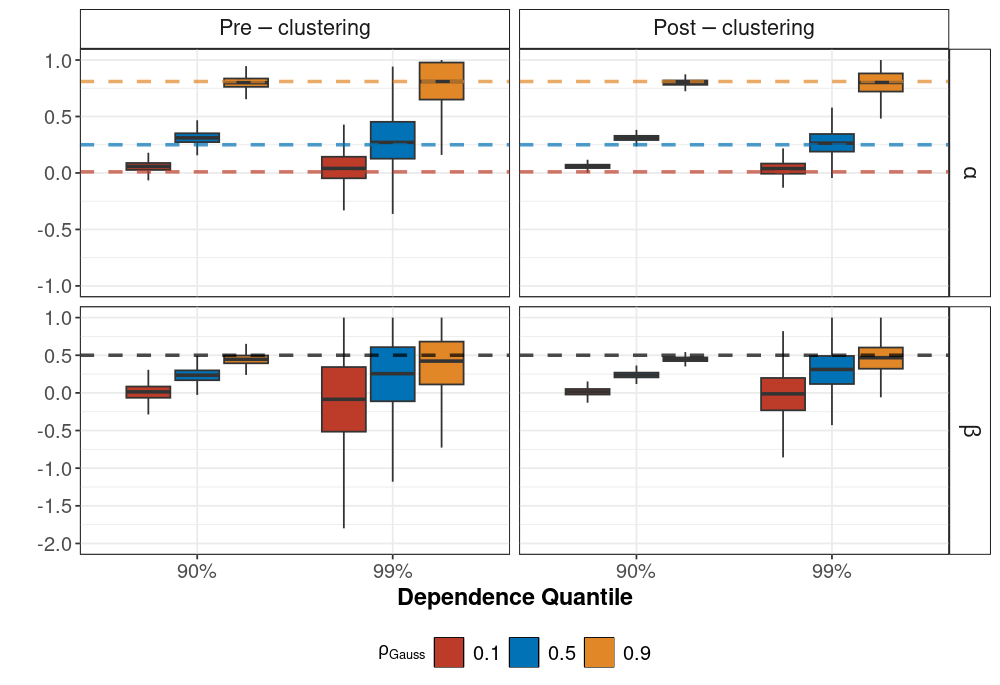
\includegraphics[width = 0.8\linewidth]{figure_1.png}
    \caption{\emph{ 
    Boxplots of estimates of $\alpha_{\mid i}$ (top) and $\beta_{\mid i}$ (bottom) for the conditional extremes model pre- and post-clustering with bivariate Gaussian data simulated at 12 sites, belonging equally to three known clusters. 
    The x-axis gives $q$, the level of the conditioning quantile used to fit the model, and the boxes are coloured by the true Gaussian copula correlation parameter, $\rho_{\text{Gauss}}^s$.
    The horizontal lines indicate the true theoretical values of $\alpha_{\mid i}$ and $\beta_{\mid i}$, with the colours for $\alpha_{\mid i}$ corresponding with the true $\rho_{\text{Gauss}}^s$ values.
    }}
   \label{fig:00_gauss_cop}
\end{figure}


\subsection{Mixture model setting}
\label{subsec:sim_mixture}

We extend our simulation design to mixtures of Gaussian and Student $t$-copulas \citep{Demarta2007-ap}, which induce asymptotic independence and asymptotic dependence, respectively, and whose dependence strength is determined by their respective correlation parameters $\rho_{\text{Gauss}}^s$ and $\rho_{\text{t}}^s \in [0, 1]$.

To obtain a sample of size $n = 1000$ from the mixture copula, at each site $s =1, \ldots, 12$, we combine $n/2 = 500$ samples from the Gaussian copula described in Section~\ref{subsec:sim_gauss} (with correlation parameter $\rhou{Gauss}^s$), and $n/2 = 500$ observations from a Student $t$-copula with 3 degrees of freedom and correlation $\rhou{t}^s$, before applying the Laplace transformation in Equation~\eqref{eq:laplace} to obtain the pairs $(Y_{1,s}, Y_{2,s})$ at site $s$.

In Section~\ref{subsubsec:sim_competing_methods}, we compare our method to the leading extremal competitor in the bivariate case \citep{Vignotto2021} and, in Section~\ref{subsubsec:sim_extension}, we show how our approach uniquely handles clustering of multivariate extremes in higher dimensions ($d > 2$).
Finally, Section~\ref{subsubsec:sim_realistic} considers a setting with $D = 60$ locations across three unequally sized clusters, and locations in the same cluster exhibiting perturbations in their correlation parameters.
Performance is evaluated using the ARI, with 500 replicated experiments per setting.

\subsubsection{Comparison to \citet{Vignotto2021}}
\label{subsubsec:sim_competing_methods}

When $d = 2$, we compare our extremal clustering method to that of \citet{Vignotto2021}.
We generate $n = 1000$ observations at $D = 12$ sites, using the mixture of Gaussian and t-copulas (with Laplace margins), as described above. 
Two clusters of sites $s = {1, \ldots, 6}$ and $s = {7, \ldots, 12}$ are defined with different values of $\rhou{t}^s$. 
We set $\rhou{t}^s = \rho_{\text{t}_1}$ for $s = 1, \ldots, 6$ and $\rhou{t}^s = \rho_{\text{t}_2}$ for $s = 7, \ldots, 12$, while $\rhou{Gauss}^s$ is the same for both clusters. 
We consider a range of extremal dependence scenarios defined over a grid of values $\left(\rhou{Gauss}^s \in \{0.1, 0.2, \ldots, 1.0\}, \rho_{\text{t}_1}^s \in \{0.1, 0.3, \ldots, 0.9\}, \rho_{\text{t}_2}^s \in \{0, 0.2, \ldots, 0.8\}\right)$.
We estimate the CE model using $q = 0.9$, and clusters were obtained using the aggregated dissimilarity matrix $M$ in Equation~\eqref{eq:aggregate_matrix}.

The results are shown in Figure~\ref{fig:01_ce_vs_vi}. 
Across the range of considered bivariate extremal dependence structures, our method consistently outperforms that of \citet{Vignotto2021}. 
Both methods have high ARI when the cluster-wise difference in $\rhou{t}^s$ is larger, since greater disparity naturally makes clusters more distinct and clustering easier. 
Both methods perform better when the Gaussian and t-copula correlations are higher.
This may be because the Gaussian copula becomes more similar to the t-copula for higher values of $\rhou{Gauss}$, thus allowing the clustering approach to focus on differences in the t-copula.

\begin{figure}[htb]
    \centering
    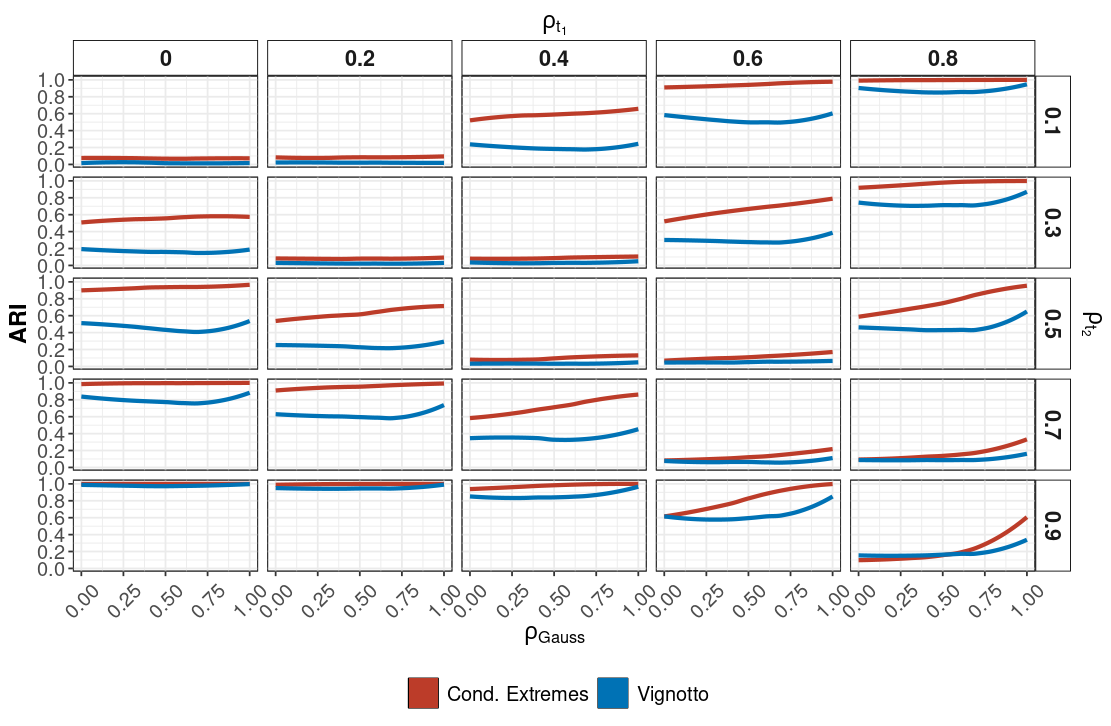
\includegraphics[width = 0.8\linewidth]{figure_2.png}
    \caption{\emph{
    Comparison of our conditional extremes-based approach and the method of \citet{Vignotto2021}.
    The x-axis represents the Gaussian correlation parameter $\rhou{Gauss}$, with facet labels indicating the t-copula correlation parameters, $\rho_{\text{t}_1}$ and $\rho_{\text{t}_2}$, for the two true clusters.
    The smoothed lines show the average ARI across bootstrap samples, for both methods, with smoothing performed using a generalised additive model.
    }}
    \label{fig:01_ce_vs_vi}
\end{figure}

\subsubsection{Extension to higher dimensions}
\label{subsubsec:sim_extension}

While the method of \citet{Vignotto2021} is restricted to $d = 2$ dimensions, our approach can be extended to $d \geq 3$ variables. 
To illustrate this, we extend the simulation study of Section~\ref{subsubsec:sim_competing_methods} by simulating at $D = 12$ locations, with two equally-sized clusters of sites each with $n = 1000$ observations per site, but now for $d = 3$ variables, using the same grid of ($\rhou{Gauss}, \rho_{\text{t}_1}, \rho_{\text{t}_2}$) values as in Section~\ref{subsubsec:sim_competing_methods}.
Our mixture copula now has three dimensions (with all pairwise correlations equal), and we fit three CE models at each site. 
Clustering is performed using the aggregated divergence matrix $M$ from Equation~\eqref{eq:aggregate_matrix}.
The results show that our proposed method performs well for $d =3$, with the same patterns in ARI emerging as in the bivariate case in Section~\ref{subsubsec:sim_competing_methods}.
In fact, performance is markedly stronger in three dimensions than in two. 
This is not surprising, as the CE fits in this setup are similar in both two and three dimensions, with the same $\rhou{t}^s$ being used across all variable pairs.
Therefore, the aggregated matrix $M$ in Equation~\eqref{eq:aggregate_matrix} is computed similarly, just averaged over more models with more data, which naturally improves clustering performance.

\begin{figure}[htb]
    \centering
    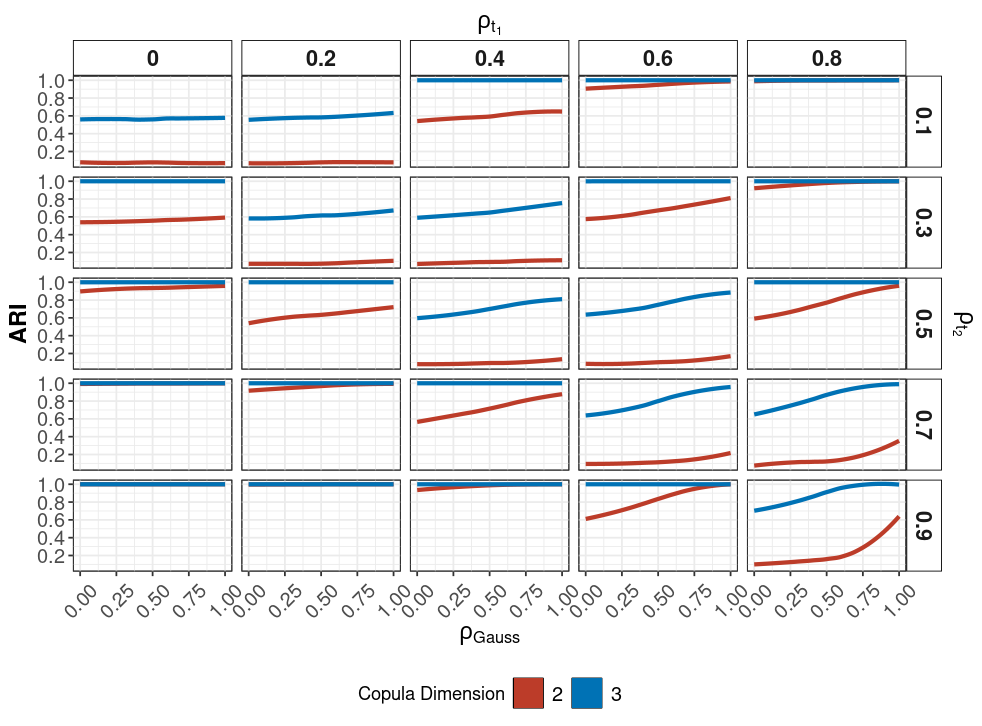
\includegraphics[width = 0.8\linewidth]{figure_3.png}
    \caption{\emph{
        Comparison of clustering performance for $d = 2$ and $d=3$ variables and two equally-sized clusters. 
        The x-axis represents the Gaussian correlation parameter $\rhou{Gauss}$ for both clusters, and the facet labels show the t-copula correlation parameters, $\rho_{\text{t}_1}$ and $\rho_{\text{t}_2}$, for the two true clusters.
        The smoothed lines show the average ARI across bootstrap samples, with smoothing performed using a generalised additive model.
    }}
   \label{fig:02_3d}
\end{figure}


% Expand to up to 5 dimensions!
To further illustrate the performance of our method in higher dimensions, we consider a specific case from the grid where $\rho_{\text{t}_1} = 0.4$ and $\rho_{\text{t}_2} = 0.5$. 
This setting presents a challenging clustering scenario in both two and three dimensions, as the cluster-wise difference in the t-copula correlation parameters is small. 
Figure~\ref{fig:02b_5d} displays the results when the dimensionality of the copula mixture is increased from $d = 2$ to $d = 5$, based on 500 simulations across all considered $\rhou{Gauss}$ values. 
Cluster accuracy improves steadily with dimension, reaching values close to 1 across all $\rhou{Gauss}$ settings when $d = 5$. 
These gains should be interpreted cautiously, since as mentioned above we use the same $\rhou{t}^s$ across all variable pairs, thus not altering the pairwise extremal dependence structure and instead increasing the amount of data as $d$ increases.
Having separate $\rhou{t}^s$ values for each variable pair would increase the complexity and signal-to-noise ratio of the clustering task, and likely reduce performance.
Nevertheless, the results demonstrate that the proposed method scales effectively to higher dimensions and performs well in multivariate settings. 

\begin{figure}[htb]
    \centering
    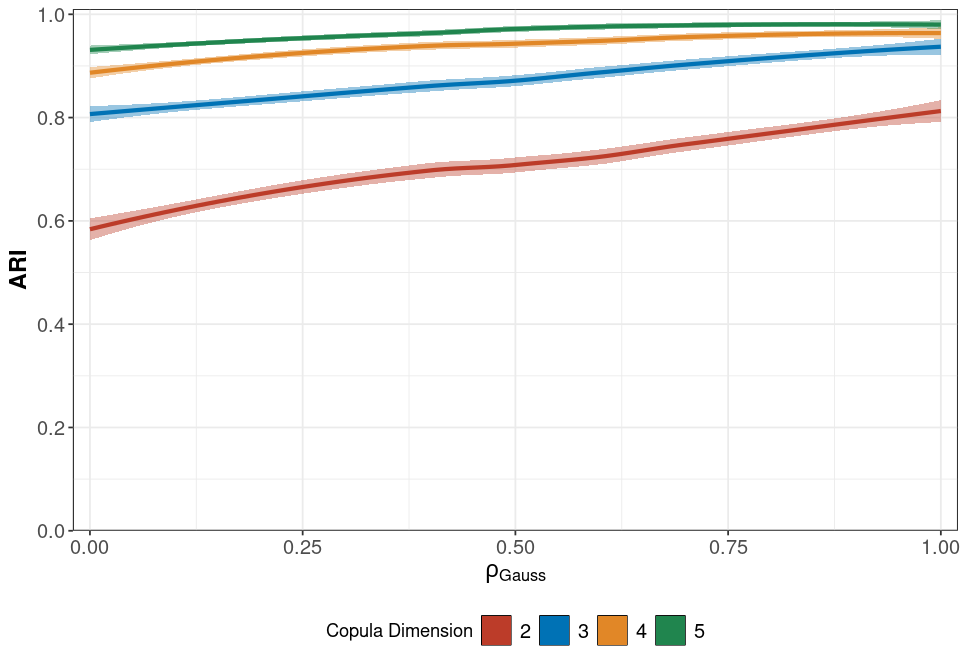
\includegraphics[width = 0.7\linewidth]{figure_4.png}
    \caption{\emph{
        Evaluation of clustering for $d = 2$ to $d = 5$ variables and two equally-sized clusters for simulations at 12 sites from a mixture of Gaussian and t-copulas.
    The t-copula correlation parameters for each true cluster were set to $\rho_{\text{t}_1} = 0.4$ and $\rho_{\text{t}_2} = 0.5$. 
A sequence of values are considered for the Gaussian correlation parameter $\rhou{Gauss}$, as represented on the x-axis.
    The smoothed lines show the average ARI and associated uncertainty across bootstrap samples, with smoothing performed using a generalised additive model.
}}
\label{fig:02b_5d}
\end{figure}

\subsubsection{Extension to more sites}
\label{subsubsec:sim_realistic}

We now design another simulation study to better mimic the structure of the Irish meteorological dataset, to be analysed in Section~\ref{sec:application}. 
Data are generated at $D = 60$ sites, each with $n = 1000$ observations of $d = 2$ variables, using the mixture of Gaussian and t-copulas.
The 60 sites are partitioned into three unequally-sized clusters of 10, 20, and 30 sites. 
At each location, the true $\rho_{\text{t}}^s$ is perturbed by adding $\text{Unif}(-0.05, 0.05)$ noise, making the clustering task more challenging.
We now have a separate t-copula correlation parameter for each of the three clusters, denoted by $\rho_{\text{t}_1}, \rho_{\text{t}_2}$, and $\rho_{\text{t}_3}$.
To reduce the dimensionality of the grid of considered copula parameter values, a constant $\rhou{Gauss} = 0.5$ is used across all sites and experiments. 

% results
The results of 500 repetitions of this simulation study are shown in Figure~\ref{fig:03_realistic}.
Similarly to the previous simulation studies, our clustering method performs well, particularly when the differences in t-copula correlation parameters between clusters are larger. 
For example, the best performance is observed where $\rho_{\text{t}_1} = 0.9, \rho_{\text{t}_2} = 0.1$, and $\rho_{\text{t}_3} = 0.5$, as the clusters are most distinct, while conversely, performance is worst for $\rho_{\text{t}_1} = 0.6, \rho_{\text{t}_2} = 0.4$, and $\rho_{\text{t}_3} = 0.5$. % \todo{Include this to aid reading of figure, is it necessary?}

\begin{figure}[htb]
    \centering
    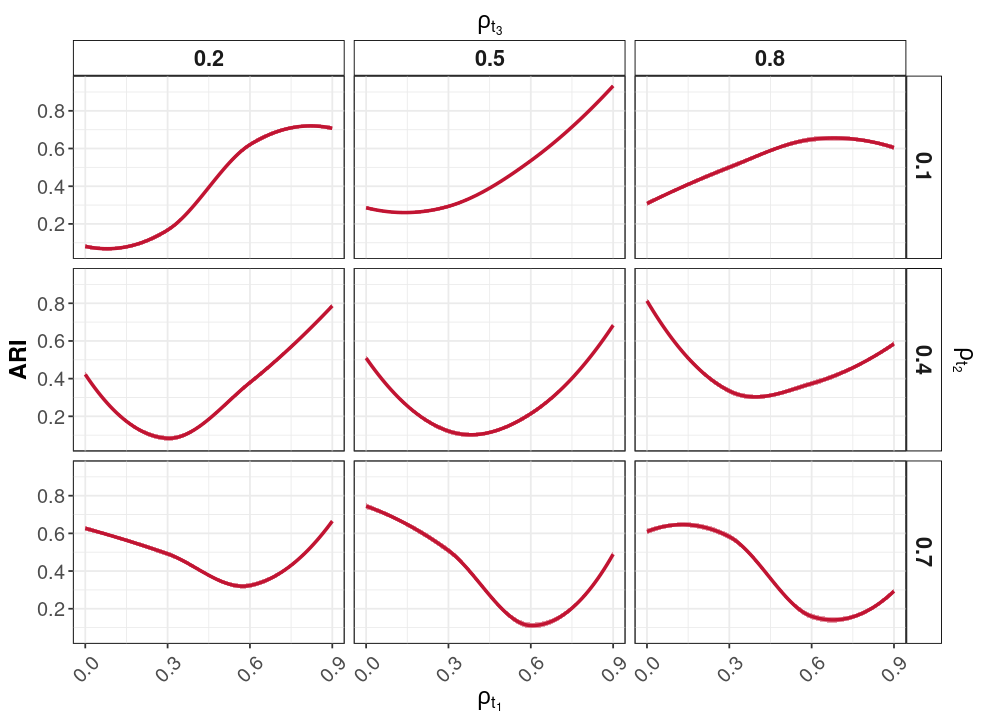
\includegraphics[width = 0.7\linewidth]{figure_5.png}
    \caption{\emph{Evaluation of clustering performance for $d = 2$ variables and three clusters of 60 locations for simulations from a mixture of Gaussian and t-copulas.
        The true x-axis and facet labels show the t-copula correlation parameters,  $\rho_{\text{t}_1}, \rho_{\text{t}_2}$, and $\rho_{\text{t}_3}$, for each of the three true clusters, for a Gaussian copula correlation of $\rhou{Gauss} = 0.5$. 
    The smoothed lines show the average ARI across bootstrap samples, with smoothing performed using a generalised additive model. 
    }}
   \label{fig:03_realistic}
\end{figure}

\section{Application to Irish meteorological data}
\label{sec:application}
% Section Intro
We now apply our extremal clustering method to meteorological observations from the Republic of Ireland. 
In Section~\ref{subsec:app_data}, we describe the precipitation and wind speed measurements used in our analysis and present exploratory analysis (using the $\chi$ statistic from Equation~\eqref{eq:chi}) on the extremal dependence between the two variables. 
In Section~\ref{subsec:app_ce}, we discuss fits of the conditional extremes (CE) model, and, in Section~\ref{subsec:app_clust}, we apply our extremal clustering approach. 

\subsection{Ireland meteorological data}
\label{subsec:app_data}

\begin{figure}[htb]
    \centering
    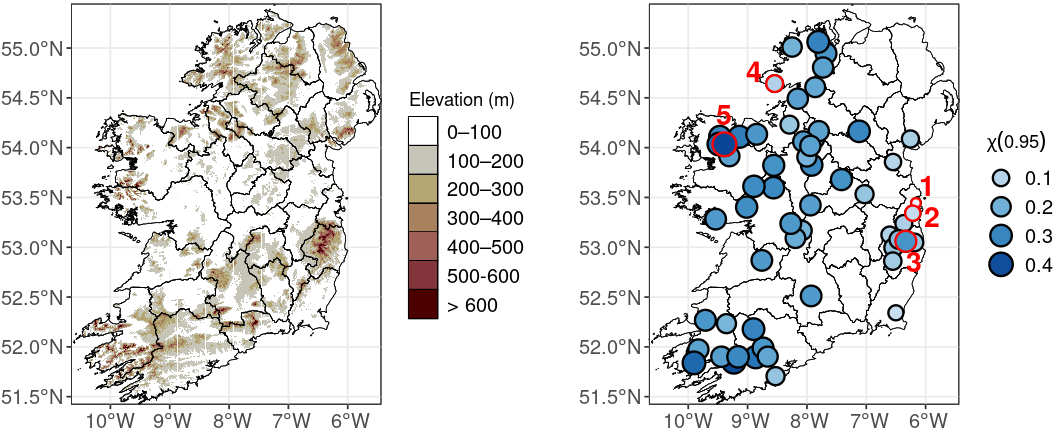
\includegraphics[width = 0.8\linewidth]{figure_6.png}
    \caption{\emph{
    Left: elevation (m) profile of Ireland.
    Right: Estimated $\chi(0.95)$ between precipitation and wind speed at all 59 locations. Darker colours and larger points indicate stronger asymptotic dependence.
    Locations in red are (1) Malahide Castle, Dublin, (2) Ringsend, Dublin, (3) Glenmacnass, Wicklow, (4) Kilcar, Donegal, and (5) Derryhillagh, Mayo.
}}
   \label{fig:chi}
\end{figure}

We analyse the joint extremal behaviour of precipitation and wind speed at $D=59$ sites across the Republic of Ireland from 1990 to 2020, inclusive. 
Precipitation and wind speed data are obtained from the Met Éireann archive \citep{metHistoricalData}, and ERA5 Reanalysis \citep{Hersbach2020}, respectively. 
Met Éireann data are irregularly spaced over space, while ERA5 provides spatial averages on a regular $0.25^{\circ} \times 0.25^{\circ}$ grid.
We match each spatial site to the grid cell in which it lies. 
The dataset spans 11,323 consecutive daily observations.

% Preprocessing
We focus on the winter months, October to March, following \citet{Vignotto2021}.
Precipitation are aggregated into weekly sums, and daily wind speed maxima are aggregated into weekly averages.
This weekly temporal scale reflects the typical lag between extreme precipitation and wind speed during storm events \citep{Bengtsson2009}, and reduces short-term temporal dependence not accounted for in our model. 
Weeks with no precipitation are excluded, resulting in 5,022 observations across all $D = 59$ sites. 

% Chi statistic
We explore the extremal dependence structure of the data using the $\chi$ statistic introduced in Equation~\eqref{eq:chi}.
Figure~\ref{fig:chi} shows empirical estimates of $\chi(0.95)$ at all 59 sites.
An elevation profile of Ireland is also shown in Figure~\ref{fig:chi}, which may help further explain some of this spatial structure.
Non-zero values are observed at almost all sites, indicating positive extremal dependence between precipitation and wind speed. 
In practical terms, this suggests that extreme wind speeds tend to be accompanied by high precipitation, and vice versa. 
A clear spatial pattern emerges: extremal dependence is strongest in the south west, with the highest values along the Atlantic coast, notably in counties Kerry, Galway, Mayo, and Donegal, and weaker along the east coast, in Dublin, Wexford, and Louth. 
The highest $\chi(0.95)$ value (0.414) is observed at Derryhillagh in Mayo (Figure~\ref{fig:chi}, location (5)), while the lowest (0.0005) is at Malahide Castle in Dublin (Figure~\ref{fig:chi}, location (1); hereafter `Malahide').

Some spatial outliers are also apparent. 
Kilcar in Donegal (Figure~\ref{fig:chi}, location (4)) has a relatively low $\chi(0.95)$ value (0.109), despite its west-coast location, while some sites in county Wicklow show unusually high values for the east, particularly Glenmacnass (Figure~\ref{fig:chi}, location (3); 0.268).
The latter may be related to the influence of the Wicklow Mountains, as reflected in the elevation profile (Figure~\ref{fig:chi}). 
It may be of interest to investigate if these outliers in $\chi(0.95)$ are reflected in the CE model parameter estimates, and whether clustering can identify them.
These results indicate distinct regional patterns of extremal dependence, as well as notable outliers, motivating the use of our extremal clustering framework to characterise and interpret this spatial structure more formally. 

\subsection{Conditional extremes estimates}
\label{subsec:app_ce}

% Procedure and results pre-clustering (choice of quantile)
We transform the precipitation and wind speed data, separately at each location, to Laplace margins, with the empirical rank transform replacing $F_{X_i}$ in Equation~\eqref{eq:laplace}.
To select an appropriate quantile level $q$ for fitting the CE model (see Section~\ref{subsec:ce_model}), we estimate the parameters $(\alpha_{\mid i}, \beta_{\mid i})$ at a sequence of levels $q$, to identify the lowest $q$ beyond which parameter estimates appear stable.
Estimates are generally stable for both models, i.e.,\@ precipitation conditional on wind speed and vice versa, down to $q = 0.85$, with similar maximum likelihood estimates across 500 bootstrap samples for $(\alpha_{\mid i}, \beta_{\mid i})$.
Threshold stability plots for the CE fits at the five locations highlighted in Figure~\ref{fig:chi} are included in Figures~\ref{fig:boot_quantiles_malahide} -- \ref{fig:boot_quantiles_derryhillagh} of the supplementary materials.
Therefore, we fix $q = 0.85$ for the subsequent analysis.
In Figure~\ref{fig:clust_sens}, we show that our estimated extremal clustering is robust to the choice of $q$, with estimates shown for $q = 0.85, 0.88$, and $0.90$.

The estimated site-wise CE parameters are shown in Figure~\ref{fig:a_b_vals}.
Although interpretation is challenging due to variability in the estimates, as with the $\chi(0.95)$ estimates (Figure~\ref{fig:chi}), we observe some evidence of increasing $\alpha_{\mid i}$ values for both variables towards the west and south.
To mitigate uncertainty and aid interpretation, we cluster the locations using our extremal clustering approach. 

\begin{figure}[htb]
    \centering
    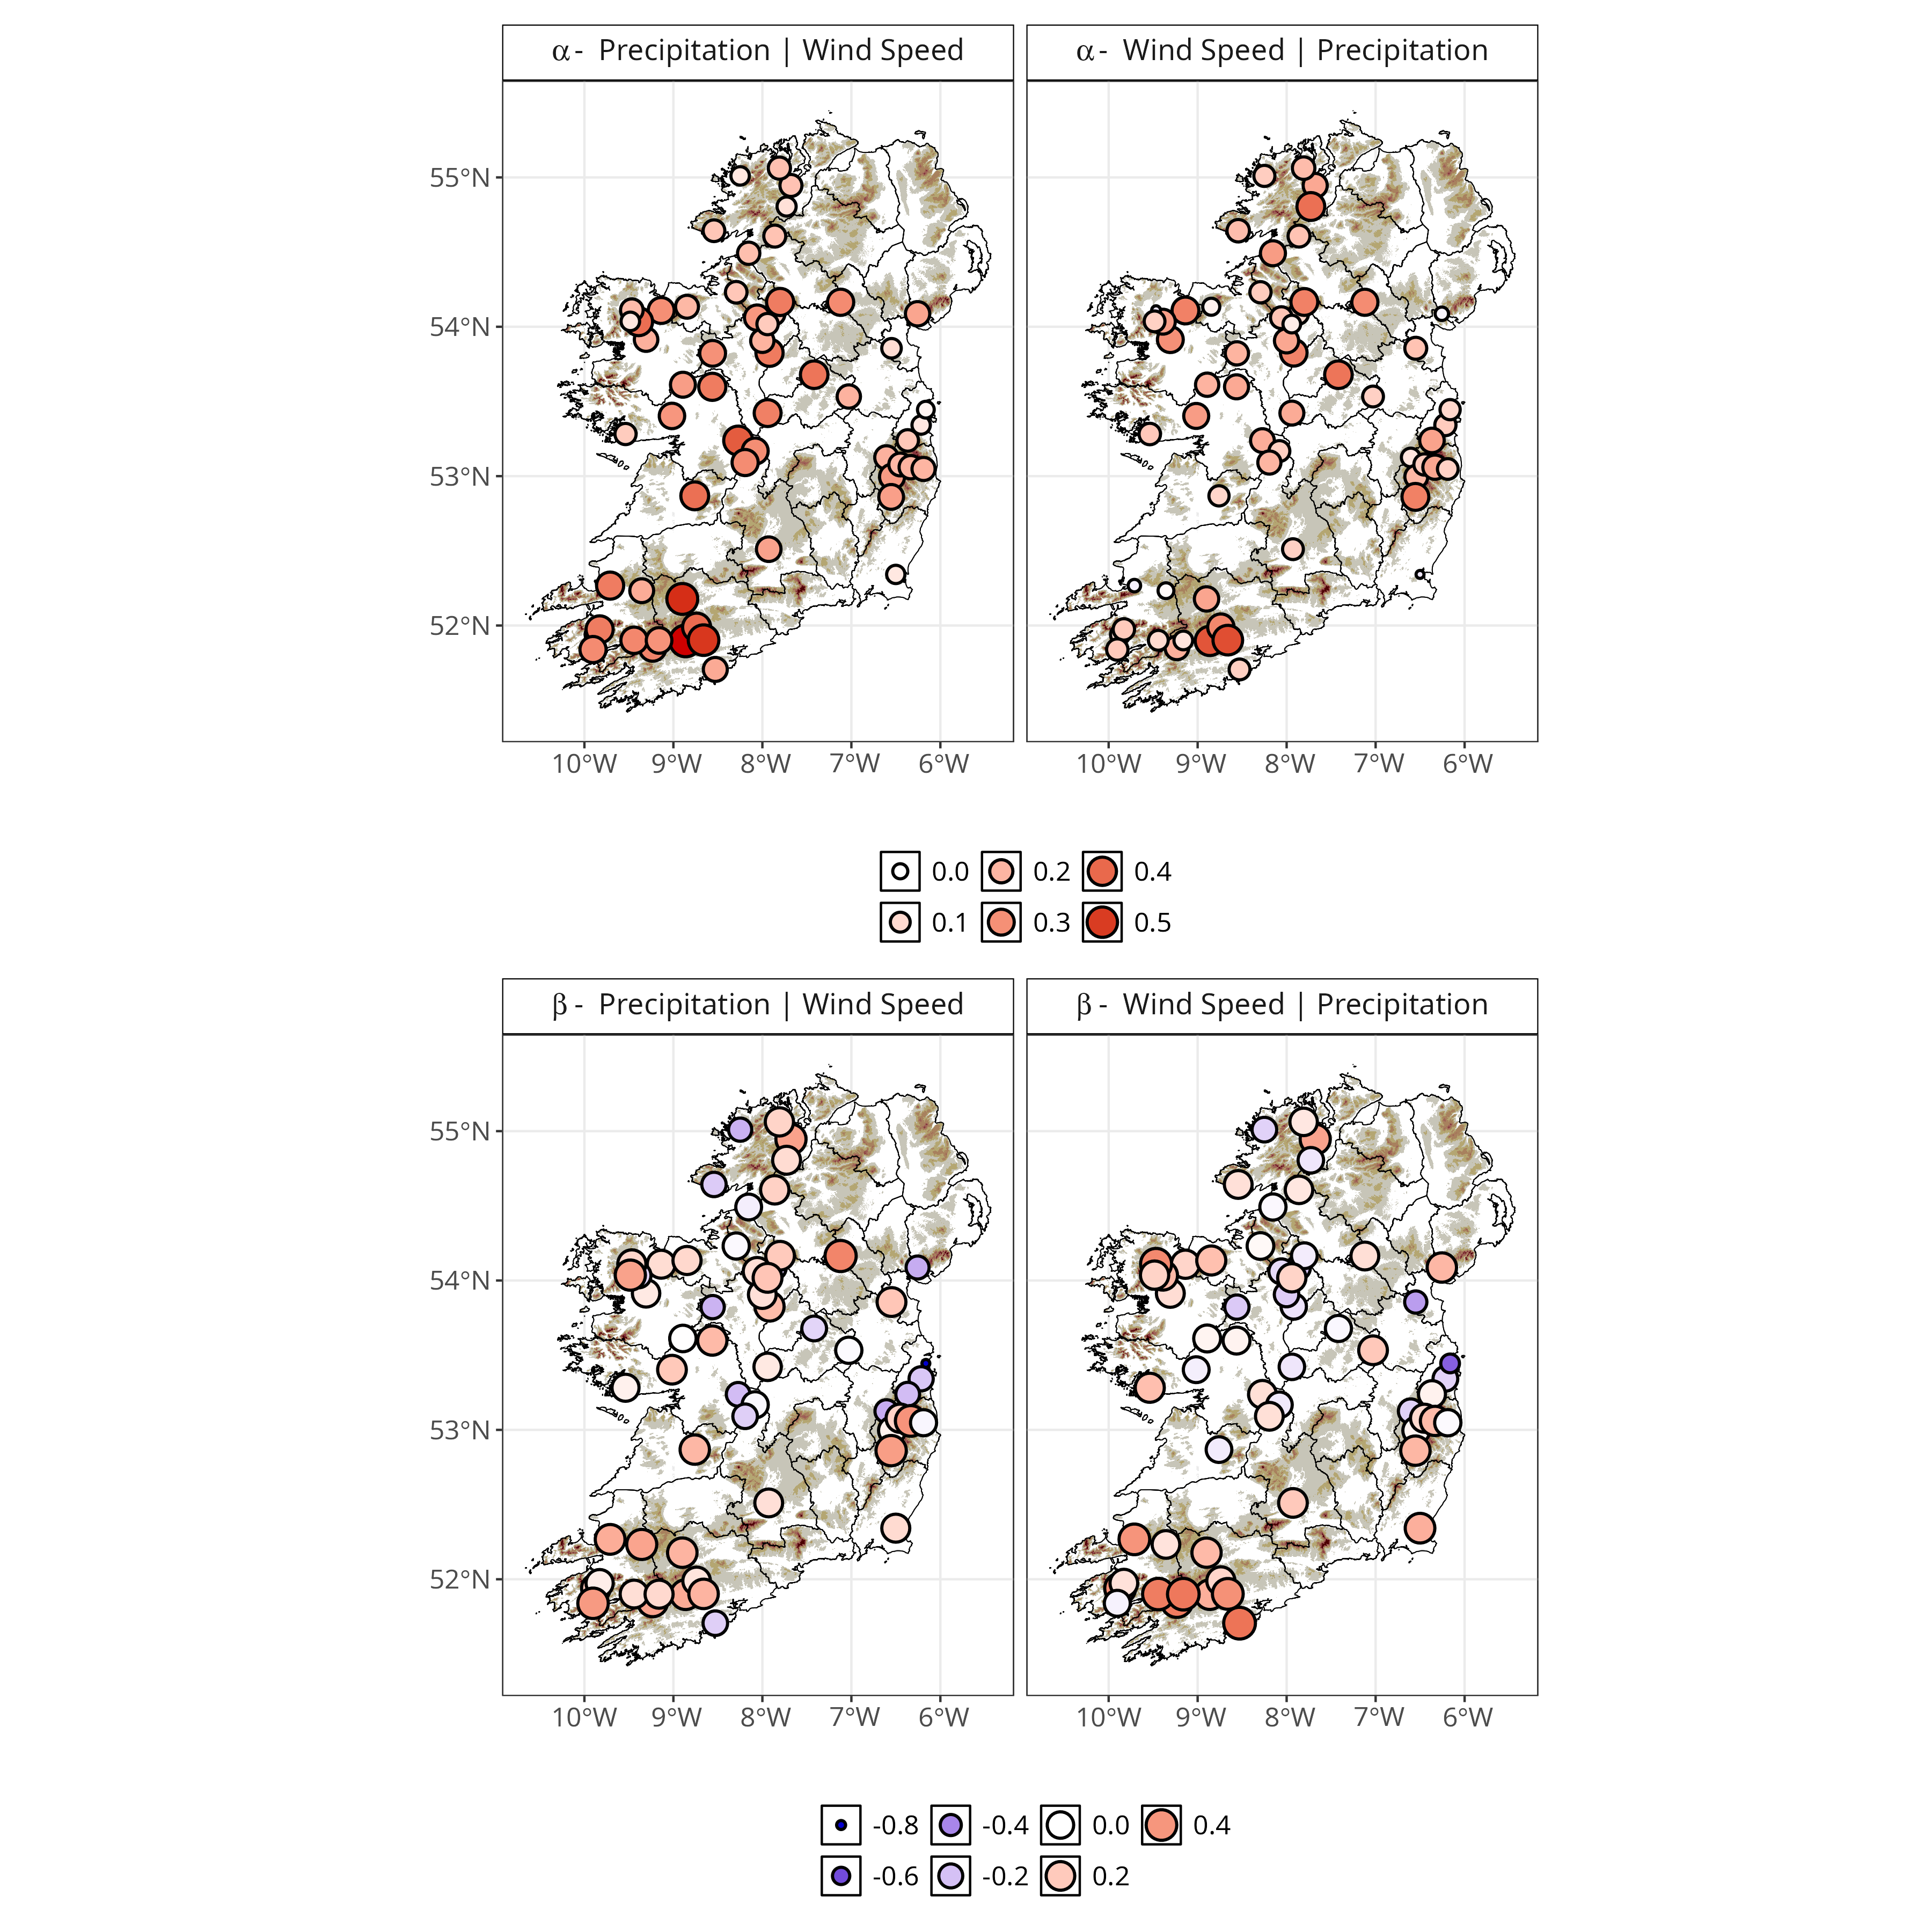
\includegraphics[width = 0.8\linewidth]{figure_7.png}
    \caption{\emph{
        Maps of site-wise estimated model parameters $\alpha_{\mid i, s}$ (top) and $\beta_{\mid i, s}$ (bottom) for precipitation conditional on wind speed (left) and wind speed conditional on precipitation (right).
        The colour scale is the same for both variables, with darker red and larger points indicating larger positive values of $\alpha$ and $\beta$, and darker blue and smaller points indicating smaller negative values.
   }}
   \label{fig:a_b_vals}
\end{figure}


\subsection{Clustering}
\label{subsec:app_clust}

We cluster the locations using the aggregated dissimilarity matrix $M$ as defined in Equation~\eqref{eq:aggregate_matrix}, and separately for each individual matrix $M^{(i)}, i = 1, 2$, as in Equation~\eqref{eq:distance_matrix}.
The number of clusters $k$ is chosen via the method in Section~\ref{subsec:clustering}, using the elbow plot of the $\mathrm{TWGSS}$. 
For all three clustering scenarios, clear elbows are observed at $k = 3$.
The elbow plots are provided in Figure~\ref{fig:elbow_plots} of the supplementary materials. 

The resulting cluster estimates are displayed in Figure~\ref{fig:clust_sol}.  
Across all three choices of dissimilarity matrix, the estimated clusters are broadly consistent, with three spatially distinct groups emerging.  
This spatial coherence is notable given that no explicit spatial information was used in model fitting or in the clustering, suggesting that the CE model parameters capture meaningful spatial structure in the extremal dependence of the data. 

When interpreting the clusters, we observe a clear contrast between the east and west coasts, separated by a central cluster.  
For precipitation conditional on wind speed, the clustering is somewhat less distinct, with the central cluster extending more extensively into parts of Galway, Mayo, and Donegal on the west coast.  
There are also notable outliers in the clusters, which we further discuss below. 

\begin{figure}[htb]
    \centering
    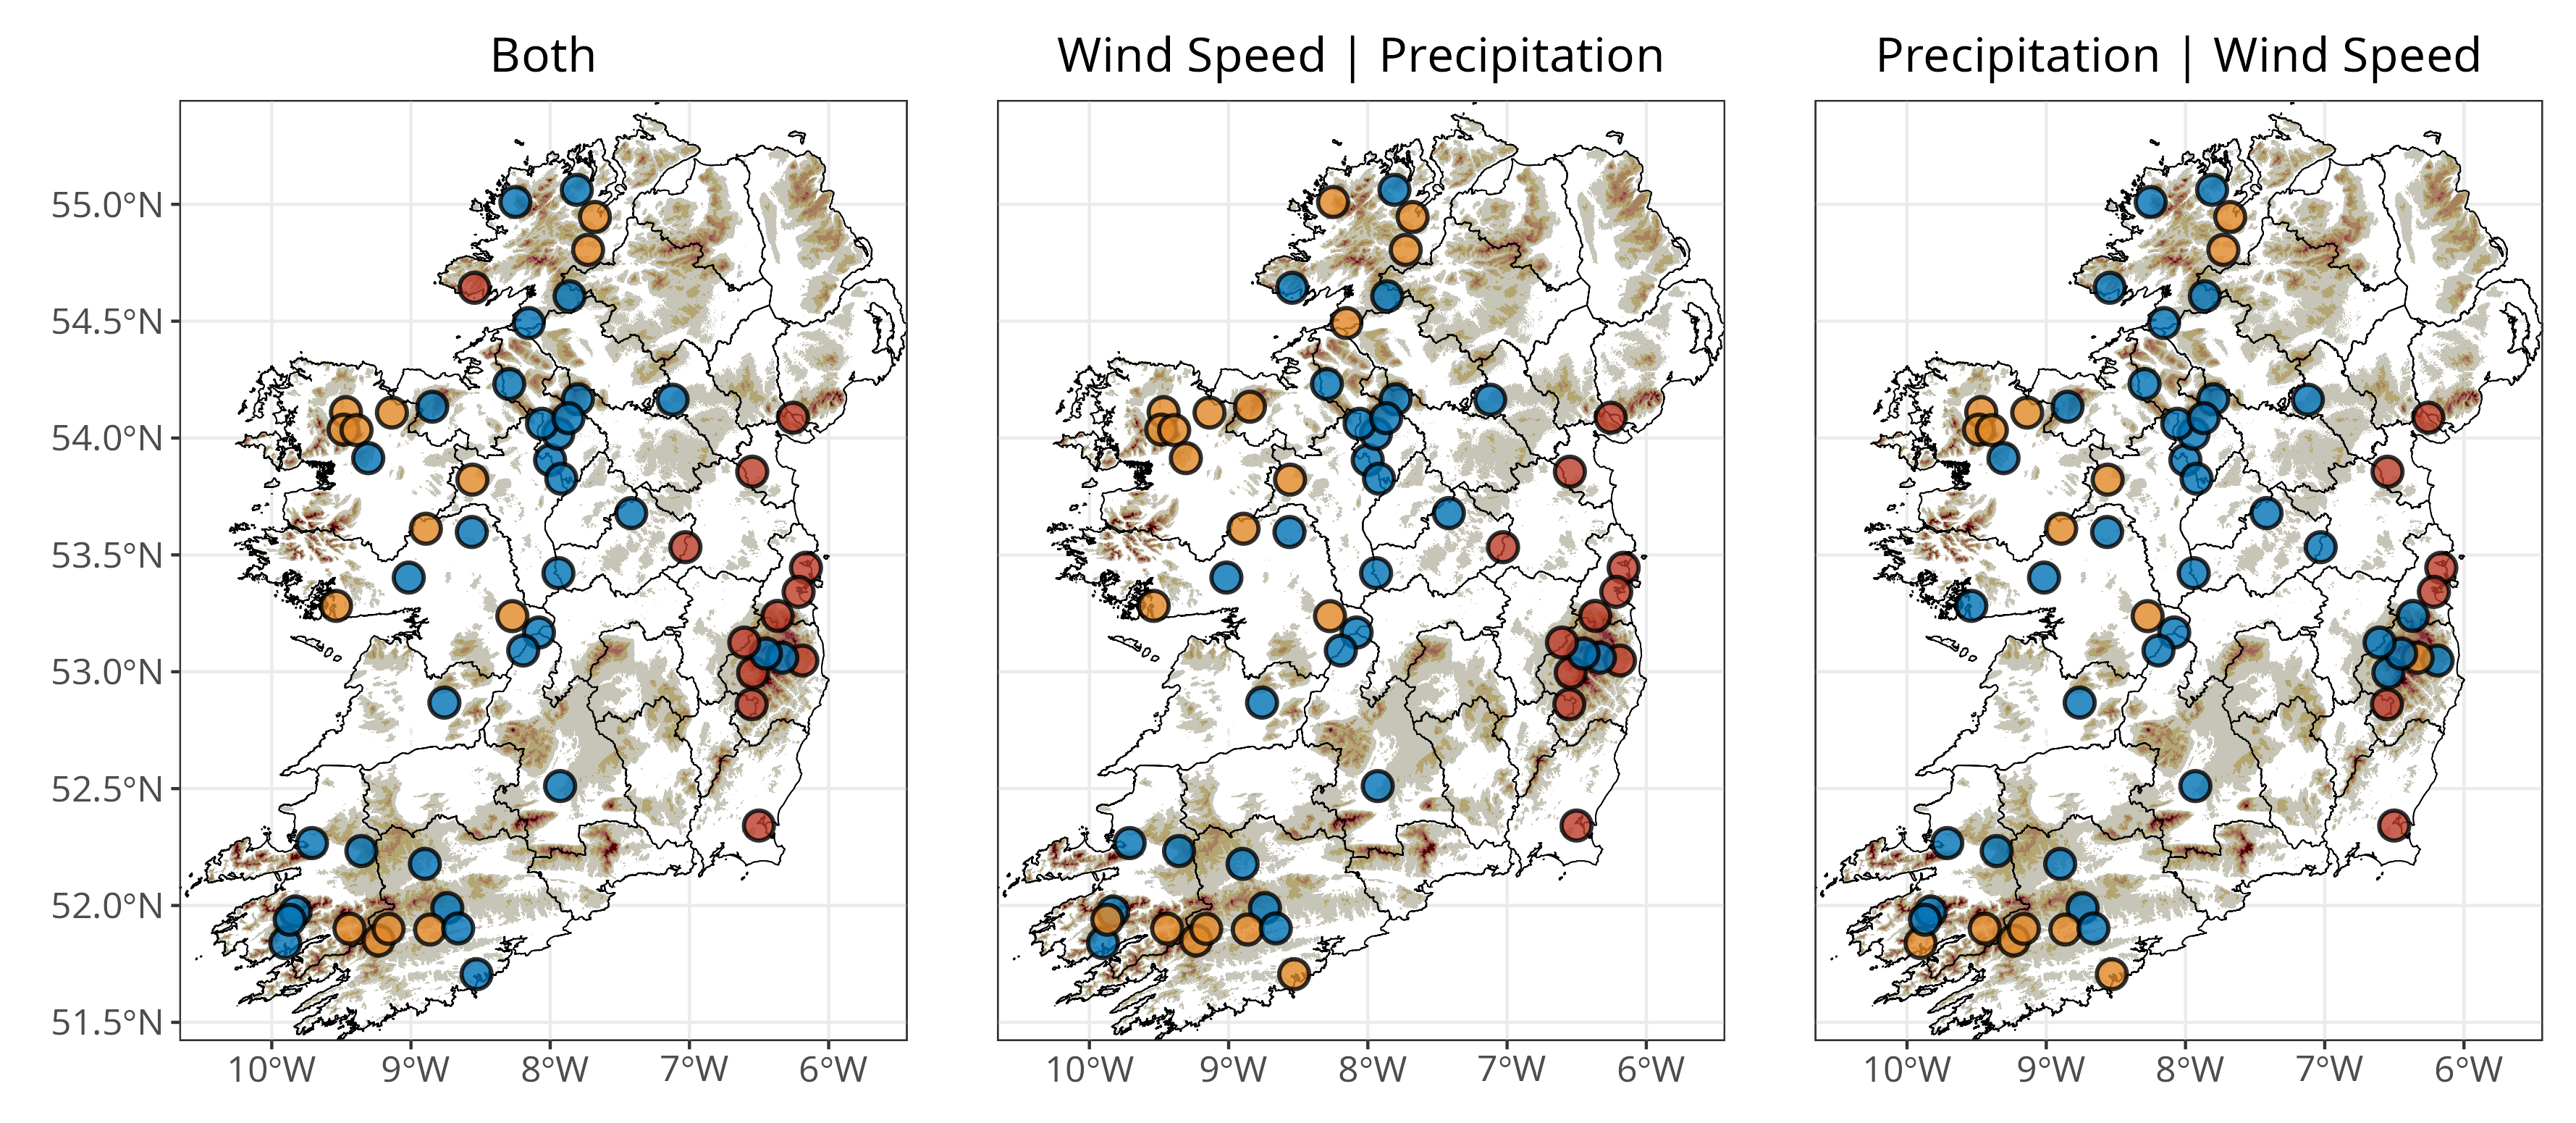
\includegraphics[width = 0.8\linewidth]{figure_8.png}
    \caption{\emph{
    Extremal cluster estimates using the dissimilarity matrix for wind speed conditional on precipitation (centre), precipitation conditional on wind speed (right), and the combined dissimilarity matrix (left). 
    Sites are coloured by cluster label.
}}
\label{fig:clust_sol}
\end{figure}

\begin{figure}[htb]
    \centering
    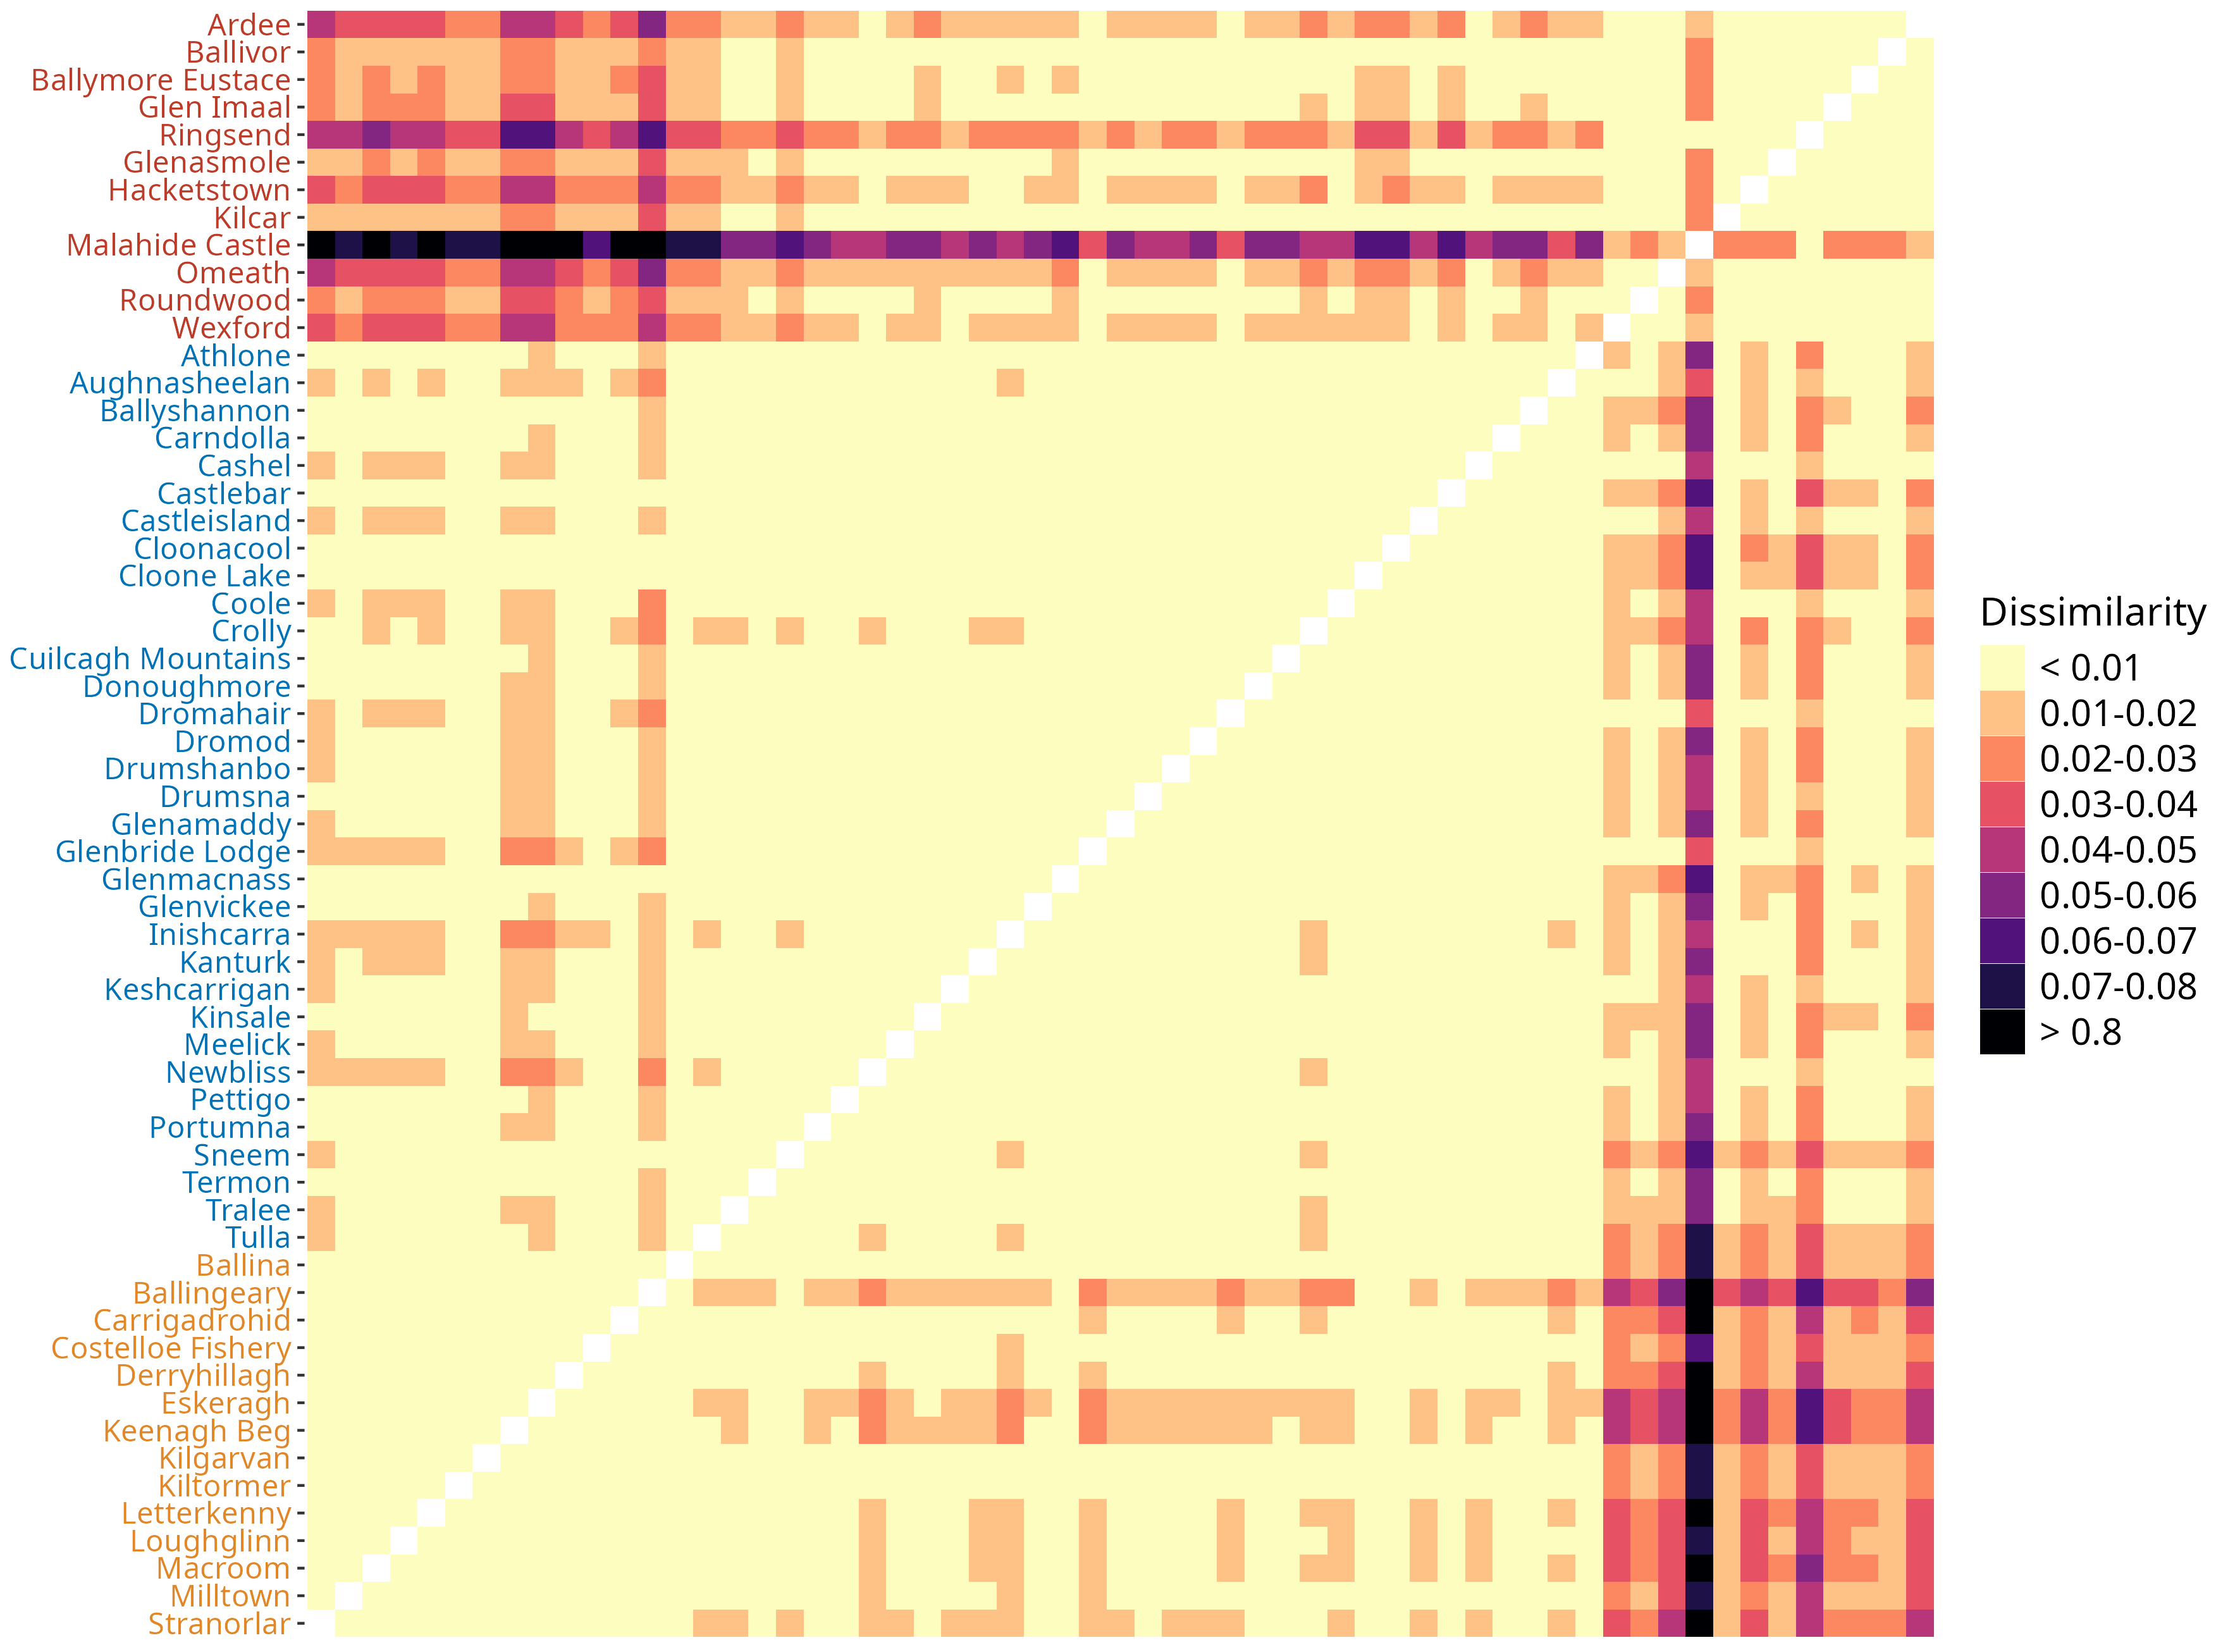
\includegraphics[width = 1.0\linewidth]{figure_9.png}
    \caption{\emph{
    Heatmap of the estimated aggregated dissimilarity matrix $M$.
The names of each site are coloured and ordered according to their estimated cluster labels, matching that of Figure \ref{fig:clust_sol}. 
The dissimilarity colour scale is shown on the right, with darker colours indicating larger values.
}}
\label{fig:dist_heatmap}
\end{figure}

% Analysis of dissimilarity matrix
In Figure~\ref{fig:dist_heatmap}, we visualise the dissimilarity matrix for the aggregated clusters (see left panel of Figure~\ref{fig:clust_sol}).
The clusters are quite distinct, with the dissimilarity between clusters being much larger than within-cluster dissimilarity, which rarely exceeds 0.01.
In particular, the difference between the eastern and western clusters is quite pronounced, with the intermediate central cluster acting as somewhat of a `buffer' between the two.
In contrast, the western and central clusters seem to be quite close, in that we observe many small inter-cluster pairwise dissimilarities between them. 
This indicates that allocation between the two is not always clear-cut and for several sites is nearly interchangeable, as observed in  the variable-specific estimated clusters in Figure~\ref{fig:clust_sol} and in the quantile sensitivity analysis in Figure~\ref{fig:clust_sens}, where membership between the two often switches. 
Also, if we only fit two clusters, we find that most of the central cluster members are assigned to the western cluster, reflecting this less obvious separation between the two compared to the more markedly different eastern cluster. 
A noticeable outlier in the dissimilarity matrix is Malahide, which we previously identified as having the lowest $\chi(0.95)$ value  in Figure~\ref{fig:chi}. 
Even within its own cluster, Malahide shows a relatively high dissimilarity to the other sites. 
Indeed, if we set $k=4$, Malahide becomes its own cluster (clustering results for $k=2$ and $k=4$ are provided in Figure~\ref{fig:cluster_dqu_k_2_4} of the supplementary materials).
Malahide also has the lowest mean weekly precipitation of any site; the second lowest is Ringsend, also in county Dublin (Figure~\ref{fig:chi} location (2)), which is the site closest to Malahide in terms of our dissimilarity measure. 
Finally, Malahide has very low $\chi(0.95)$ (Figure~\ref{fig:chi}) and $\alpha_{\mid i}$ (Figure~\ref{fig:a_b_vals}) estimates. 
Together, this may explain why we observe such outlying behaviour for Malahide.
Finally, Kilcar in County Donegal is the member of the eastern cluster with the smallest dissimilarity to the western cluster members.
This may reflect its geographic location in northwest Ireland, despite it's low $\chi(0.95)$ value (Figure~\ref{fig:chi}) relative to other west-coast sites.

\begin{figure}[htb]
    \centering
    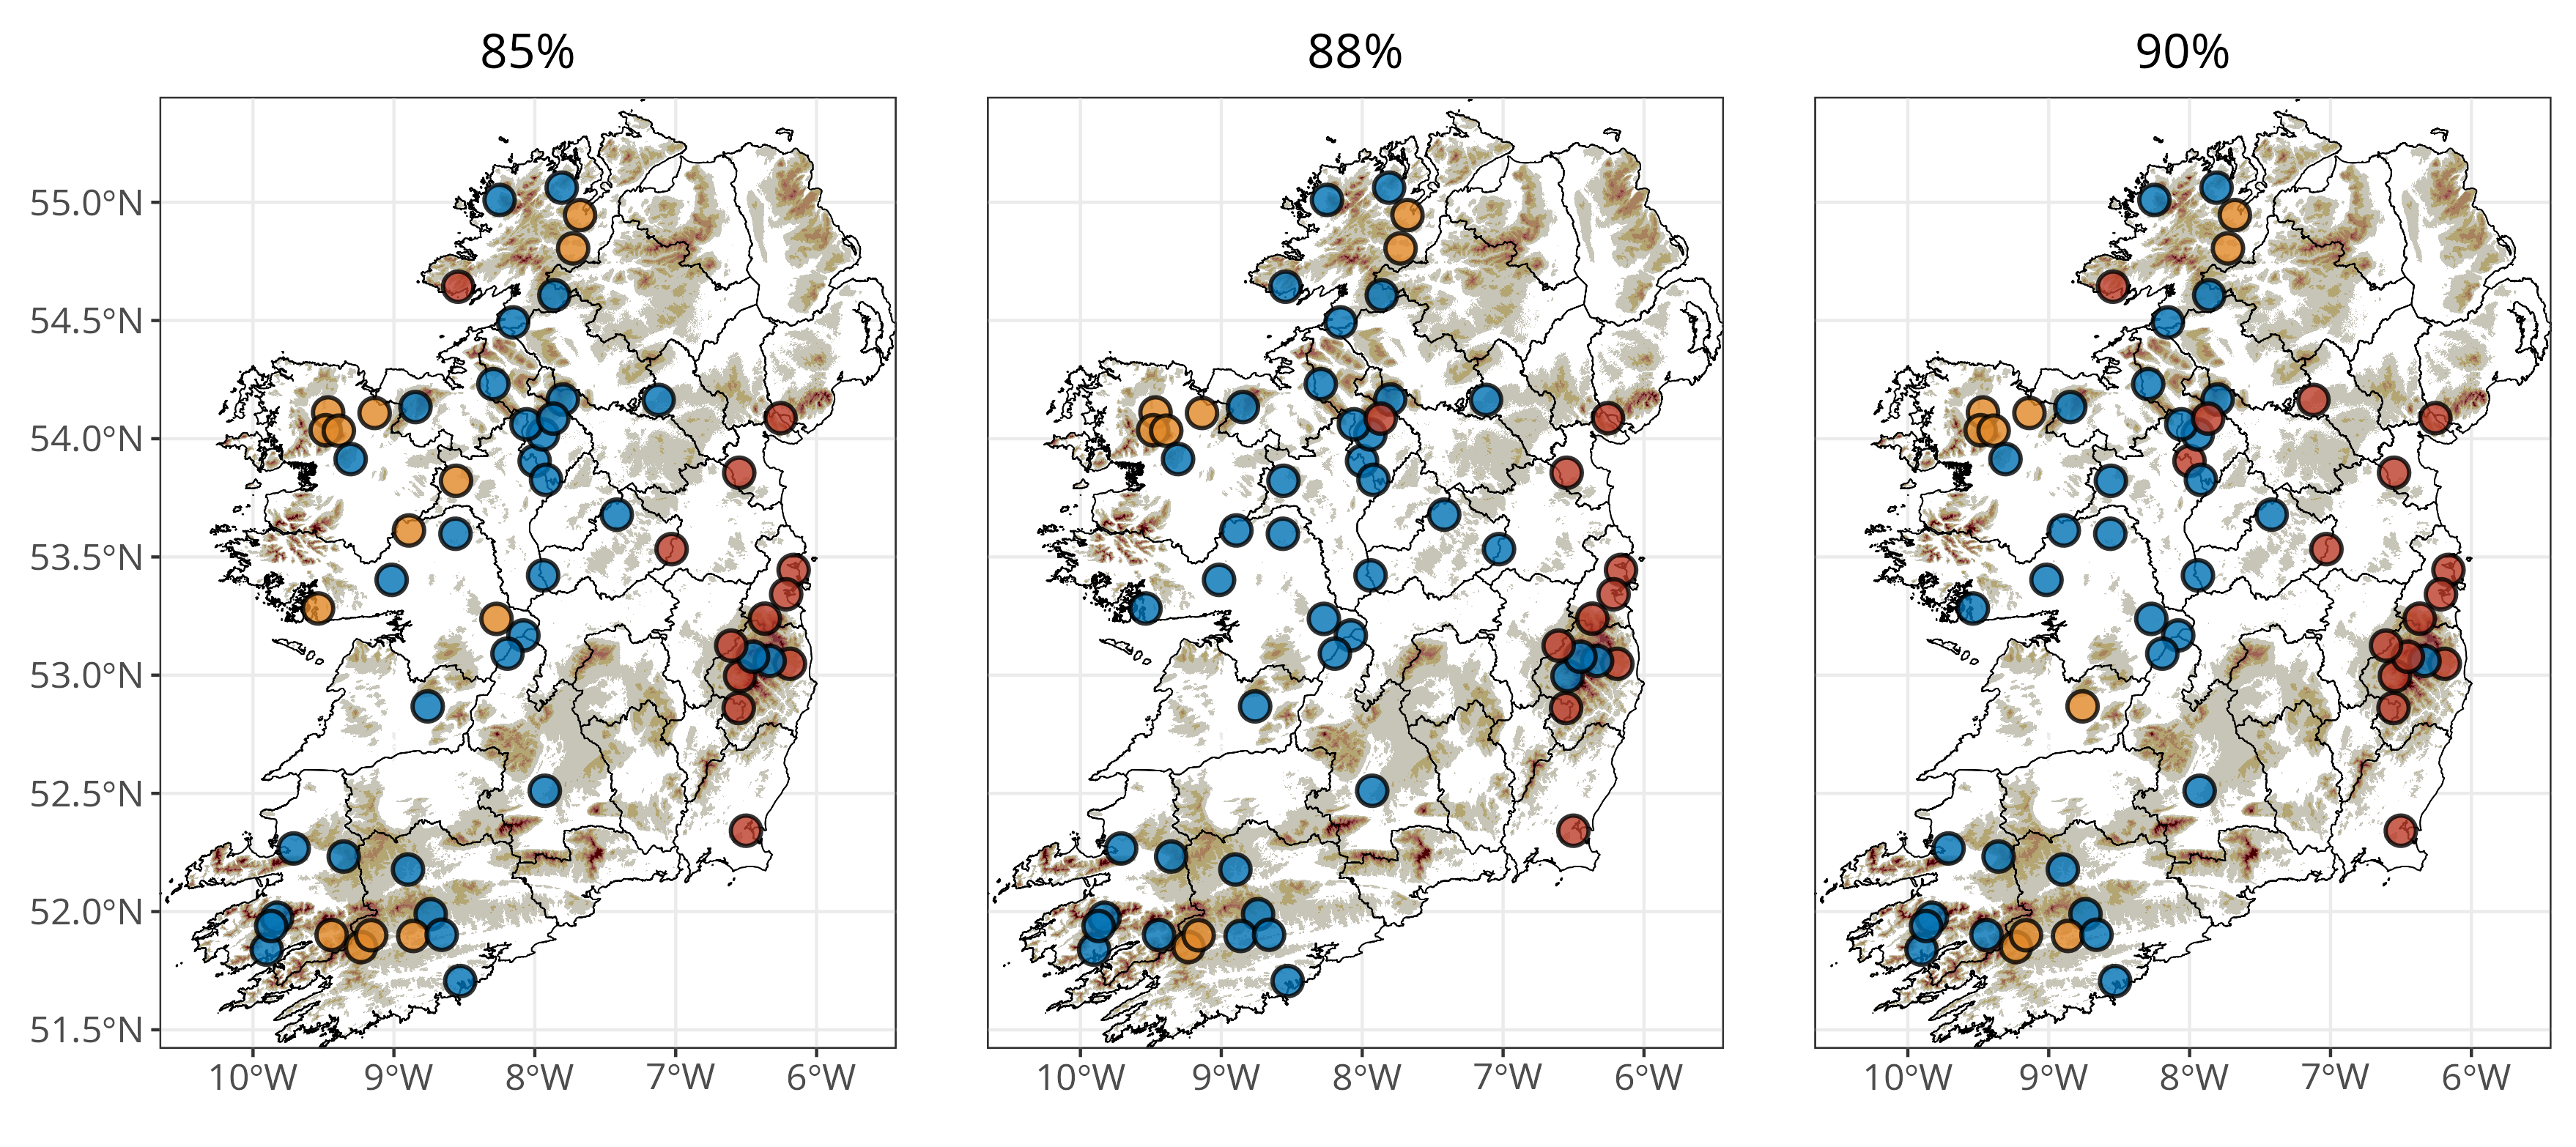
\includegraphics[width = 0.85\linewidth]{figure_10.png}
    \caption{\emph{
    Estimated extremal clusters with the conditional extremes model parameters estimated at $q = 0.85, q = 0.88$ and $q = 0.9$ quantiles, using the aggregated dissimilarity matrix. 
    Sites are coloured by cluster label. 
}}
\label{fig:clust_sens}
\end{figure}


% Sensitivity Analysis (to choice of DQU)
We perform a sensitivity analysis of the estimated clusters (with the aggregated dissimilarity matrix) to the choice of quantile level $q \in \{0.85, 0.88, 0.90\}$, in Figure~\ref{fig:clust_sens}.
The estimated clusters are similar across the three values of $q$, with some small differences. 
Noticeably, the earlier identified outlier at Kilcar in county Donegal is assigned to the eastern cluster when $q = 0.85$ and $q = 0.90$, but to the central cluster when $q = 0.88$.
Also, there are more sites in the western cluster when $q = 0.85$, with some sites moving to the central cluster for $q = 0.88$.
Interestingly, some of these sites then move back to the western cluster for $q = 0.90$.
Apart from these observations, the estimated clusters are generally quite similar across the three quantile levels, and so we conclude that our clustering method is relatively robust to the choice of quantile level.

\section{Discussion}
\label{sec:discuss}

% Quick summary
In this paper, we introduced a novel method for clustering multivariate extremes.
We proposed the expected conditional $\JSGa{}$ divergence \citep{Nielsen2019} as a measure of dissimilarity between multivariate conditional extremes (CE) models \citep{Heffernan2004}.
We leveraged the commonly-applied working Gaussian assumption to derive a closed-form expression for the $\JSGa{}$ divergence.
Efficient k-medoids clustering was then performed on the dissimilarity matrix derived from this measure. 
In our simulation study, a bivariate Gaussian copula example illustrated that our clustering method reduces parameter uncertainty and bias when the CE model is re-fitted with data pooled post-clustering.
Using mixtures of Gaussian and $t$-copulas, we showed that our method outperforms the method of \citet{Vignotto2021} across a range of bivariate extremal dependence scenarios.
Our method was also shown to be uniquely extendable to $d > 2$ dimensions. 
We applied our extremal clustering method to Irish meteorological data, consisting of 59 locations with weekly rainfall and wind speed observations.
Without explicitly incorporating spatial information, three clusters with distinct spatial patterns were identified, with well separated clusters representing the east and west coasts and the centre of Ireland.

% Extension
While we focused on a spatial application in this work, our method is more generally applicable to any setting where clustering of multivariate extremal dependence is desired.
For instance, it could be applied to clinical trial or public health data to cluster patients based on the tail dependence structure of their symptoms or biomarker measurements.
A neuroscience application was explored in \citet{Talento2025}, where the CE framework was used to highlight differences in the tail dependence of electroencephalogram (EEG) signals for seizure-prone and seizure-absent subjects. 
However, they used pre-defined clusters. Hence, we may expect our approach to be useful in similar applications, to identify subjects who have undergone extreme brain events, e.g., seizures.
In financial applications, we could cluster time periods according to the extremal dependence of log-returns of different assets, offering potential insights for portfolio management and risk assessment.

% Limitations: Gaussian assumption
While the residual Gaussian assumption on which our method relies may not hold for all datasets, our clustering approach showed good performance for all settings in Section~\ref{sec:sim}.
A possible alternative is to employ the generalised and asymmetric multivariate Gaussian distribution used in \citet{Farrell2025}. 
While this does not permit a closed-form divergence, our extremal clustering method could still be used, with costly numerical techniques used to estimate the dissimilarity matrix.
Indeed, if choosing to forgo this Gaussian assumption, it may be preferable to use the standard Jensen-Shannon divergence in place of the $\JSGa{}$ divergence, since the former is bounded \citep{Thiagarajan2025}.

% Limitations: Uncertainty
Another important limitation of our method is in its treatment of uncertainty.
We do not propagate uncertainty in the CE model estimates through to the clustering. 
To account for this, one possible approach is to use the bootstrap method of \citet{Heffernan2004} to generate samples of CE model estimates, and compute our dissimilarity matrix for each sample. 
We could then produce a distribution of dissimilarity matrices, and use these to compute a distribution of estimated clusters.
However, this would be computationally expensive, and so would compromise one of the main advantages of our method, namely its computational efficiency.

% Future work
In this work, we implicitly assume spatial stationarity in the extremal dependence structure, as we fit a separate CE model at each location.
Extensions of the CE model have been proposed, such as those incorporating covariates \citep{Richards2023} and spatio- and spatio-temporal representations of the CE parameters \citep{Simpson2021, Wadsworth2022}.
These could be incorporated into our clustering framework, but care must be taken to ensure that the residual Gaussian assumption still holds, or that an appropriate alternative dissimilarity is used, as discussed above.
Another approach to dealing with the uncertainty in the clustering solution would be to adopt a Bayesian perspective.
By placing priors on the CE model parameters, we could obtain posterior distributions for these parameters, which could be used to compute a distribution of dissimilarity matrices and clustering solutions.
Approaches such as that of \citet{Rohrbeck2021} have used a Reversible-Jump MCMC scheme to perform Bayesian clustering for spatial extremes, which does not require the number of clusters to be specified in advance.



% \section*{Acknowledgements}
% 
% \if0\blind
% {%
% Patrick O'Toole is supported by a scholarship from the EPSRC Centre for Doctoral Training in Statistical Applied Mathematics at Bath (SAMBa), under the project EP/S022945/1.
% We acknowledge the use of the ERA5 reanalysis dataset, available from the Copernicus Climate Change Service (C3S) Climate Data Store (CDS) (\url{https://cds.climate.copernicus.eu/}). 
% We also acknowledge the use of the Irish meteorological dataset obtained from Met Éireann (\url{https://www.met.ie/climate/available-data/historical-data}).
% } 
% \else
% {%
% We acknowledge the use of the ERA5 reanalysis dataset, available from the Copernicus Climate Change Service (C3S) Climate Data Store (CDS) (\url{https://cds.climate.copernicus.eu/}). 
% We also acknowledge the use of the Irish meteorological dataset obtained from Met Éireann (\url{https://www.met.ie/climate/available-data/historical-data}).
% }
% \fi


\begin{center}
{\large\bf SUPPLEMENTARY MATERIAL}
\end{center}

\begin{description}

  \item[PDF Supplement:] This supplement contains additional plots for the motivating data application in Section~\ref{subsec:app_clust} of the main paper, including elbow plots for choosing the number of clusters, clustering solutions for $k=2$ and $k=4$ clusters, and threshold stability plots for the conditional extremes model fits for the five locations highlighted in Figure~\ref{fig:chi}.

  \item[Data and R code:] The proposed methods are made available in an R package (link omitted for blind review).
    The analysis code used in the paper and the data are available upon request from the corresponding author.

\end{description}

% \typeout{=== TEX DIAGNOSTIC: before checking .bbl ===}
% \IfFileExists{manuscript_anonymous.bbl}{%
%   \typeout{=== TEX DIAGNOSTIC: BBL FILE FOUND ===}%
% }{%
%   \typeout{=== TEX DIAGNOSTIC: BBL FILE NOT FOUND ===}%
% }
% \typeout{=== TEX DIAGNOSTIC: after check ===}

% \bibliographystyle{apalike}
{\small
% \bibliography{library.bib}
\documentclass[preprint,12pt,authoryear]{elsarticle}
\usepackage{amsmath}
\usepackage{graphicx}
\RequirePackage{amsthm,amsmath,multirow,amsfonts,bbm,amssymb,xcolor}
\usepackage{mathtools}  % must be loaded before \DeclarePairedDelimiter

\usepackage{url}

\PassOptionsToPackage{unicode}{hyperref}
\PassOptionsToPackage{hyphens}{url}
\PassOptionsToPackage{dvipsnames,svgnames,x11names}{xcolor}

\usepackage{iftex}
\ifPDFTeX
  \usepackage[T1]{fontenc}
  \usepackage[utf8]{inputenc}
  \usepackage{textcomp} % provide euro and other symbols
\else % if luatex or xetex
  \usepackage{unicode-math}
  \defaultfontfeatures{Scale=MatchLowercase}
  \defaultfontfeatures[\rmfamily]{Ligatures=TeX,Scale=1}
\fi
\usepackage{lmodern}
\ifPDFTeX\else  
\fi
% Use upquote if available, for straight quotes in verbatim environments
\IfFileExists{upquote.sty}{\usepackage{upquote}}{}
\IfFileExists{microtype.sty}{% use microtype if available
  \usepackage[]{microtype}
  \UseMicrotypeSet[protrusion]{basicmath} % disable protrusion for tt fonts
}{}
\makeatletter
\@ifundefined{KOMAClassName}{% if non-KOMA class
  \IfFileExists{parskip.sty}{%
    \usepackage{parskip} % begin paragraphs with empty line rather than indent
  }{% else
    \setlength{\parindent}{0pt}
    \setlength{\parskip}{6pt plus 2pt minus 1pt}}
}{% if KOMA class
  \KOMAoptions{parskip=half}}
\makeatother
\usepackage{xcolor}
\setlength{\emergencystretch}{3em} % prevent overfull lines
\setcounter{secnumdepth}{5}
% Make \paragraph and \subparagraph free-standing
\makeatletter
\ifx\paragraph\undefined\else
  \let\oldparagraph\paragraph
  \renewcommand{\paragraph}{
    \@ifstar
      \xxxParagraphStar
      \xxxParagraphNoStar
  }
  \newcommand{\xxxParagraphStar}[1]{\oldparagraph*{#1}\mbox{}}
  \newcommand{\xxxParagraphNoStar}[1]{\oldparagraph{#1}\mbox{}}
\fi
\ifx\subparagraph\undefined\else
  \let\oldsubparagraph\subparagraph
  \renewcommand{\subparagraph}{
    \@ifstar
      \xxxSubParagraphStar
      \xxxSubParagraphNoStar
  }
  \newcommand{\xxxSubParagraphStar}[1]{\oldsubparagraph*{#1}\mbox{}}
  \newcommand{\xxxSubParagraphNoStar}[1]{\oldsubparagraph{#1}\mbox{}}
\fi
\makeatother

% NOTE: To produce blinded version, replace "0" with "1" below.
% \newcommand{\blind}{0}
\newcommand{\blind}{1}
\usepackage{rotating}

% DON'T change margins - should be 1 inch all around.
\addtolength{\oddsidemargin}{-.5in}%
\addtolength{\evensidemargin}{-1in}%
\addtolength{\textwidth}{1in}%
\addtolength{\textheight}{1.7in}%
\addtolength{\topmargin}{-1in}%

\newcommand{\red}{\textcolor{red}}

%%%% Non-template packages %%%%
\usepackage{titlesec} % Adjust spacing for sections
\usepackage{tikz}
\usepackage{amsfonts}
\usepackage{bbm}
\usepackage{pdflscape}
\usepackage{caption}
\usepackage{subcaption}
\usepackage{pdfpages}
\usepackage{setspace} 
\usepackage{booktabs}
\usepackage{longtable}
\usepackage{float}
\usepackage{tikz}
\usepackage[colorlinks=true,citecolor=blue, linkcolor=blue]{hyperref}
\usepackage{multirow}
\usepackage{algorithm}
\usepackage{algpseudocode}
\usepackage[defaultlines=2,all]{nowidow} % prevent widows and orphans
\usepackage{enumitem} % inline enumeration
\usepackage{xr-hyper}
\usepackage{subfiles} % for loading supplementary material

% penalties for breaking equations
\relpenalty=10000
\binoppenalty=10000

% Define a custom note command for general notes
\newcommand{\mynote}[1]{\todo[color=yellow!40,inline]{#1}}

% Define custom maths equations 
\DeclareMathOperator{\KL}{KL}
\DeclareMathOperator{\JS}{JS}
\DeclareMathOperator*{\argmin}{arg\,min}
\DeclarePairedDelimiter\abs{\lvert}{\rvert}%
\DeclareMathOperator{\EX}{\mathbb{E}}% expected value
\newcommand{\JSGa}{\mathop{\mathrm{JS}^{\mathrm{G}_{\lambda}}}\nolimits}
\newcommand{\cJSGa}[1]{\mathop{\mathrm{cJS}_{i, #1}^{\mathrm{G}_{\lambda}}}\nolimits}
\newcommand{\eJSGa}[1]{\mathop{\mathrm{eJS}_{i, #1}^{\mathrm{G}_{\lambda}}}\nolimits}
\DeclareRobustCommand{\eJSGai}{\mathop{\mathrm{eJS}^{\mathrm{G}_{\lambda}}}\nolimits}
\DeclareMathOperator{\GJS}{\mathrm{JS}^{\mathrm{G}}}
\DeclareMathOperator{\CE}{\mathrm{CE}}
\newcommand{\rhou}[1]{\rho_{\text{#1}}}
\newcommand\numberthis{\addtocounter{equation}{1}\tag{\theequation}}

\newcommand{\mvmean}[1]{\boldsymbol{\alpha}_{\mid i, #1} y + y^{\boldsymbol{\beta}_{\mid i, #1}} \boldsymbol{\mu}_{\mid i, #1}}
\newcommand{\mvcov}[1]{\left(y^{\boldsymbol{\beta}_{\mid i, #1}}\right)^{\mathrm{T}} \Sigma_{\mid i, #1} y^{\boldsymbol{\beta}_{\mid i, #1}}}


\usepackage{xr-hyper}
\externaldocument{supplementary_material_anonymous}

\begin{document}

\def\spacingset#1{\renewcommand{\baselinestretch}%
{#1}\small\normalsize} \spacingset{1}

%%%%%%%%%%%%%%%%%%%%%%%%%%%%%%%%%%%%%%%%%%%%%%%%%%%%%%%%%%%%%%%%%%%%%%%%%%%%%%

\if0\blind
{
  \title{\bf Clustering of multivariate tail dependence using conditional methods}
  \author{%
  Patrick O'Toole\thanks{Patrick O'Toole is supported by a scholarship from the EPSRC Centre for Doctoral Training in Statistical Applied Mathematics at Bath (SAMBa), under the project EP/S022945/1.}\\
  Department of Mathematical Sciences, University of Bath, UK
  \and
  Christian Rohrbeck\\
  Department of Mathematical Sciences, University of Bath, UK 
  \and
  Jordan Richards\\
  School of Mathematics \\
  and Maxwell Institute for Mathematical Sciences, \\
  University of Edinburgh, UK
  }
  \maketitle
} \fi

\if1\blind
{
  \begin{center}
    {\LARGE\bf Title}
\end{center}
  \medskip
} \fi


\begin{abstract}
  The conditional extremes (CE) framework has proven useful for analysing the joint tail behaviour of random vectors.
  However, when applied across many locations or variables, it can be difficult to interpret or compare the resulting extremal dependence structures, particularly for high dimensional vectors. 
  To address this, we propose a novel clustering method for multivariate extremes using the CE framework.
  Our approach introduces a closed-form, computationally efficient dissimilarity measure for multivariate tails, based on the skew-geometric Jensen-Shannon divergence, and is applicable in arbitrary dimensions.
  Applying standard clustering algorithms to a matrix of pairwise distances, we obtain interpretable groups of random vectors with homogeneous tail dependence.
  Simulation studies demonstrate that our method outperforms existing approaches for clustering bivariate extremes, and uniquely extends to the multivariate setting. 
  In our application to Irish meteorological data, our clustering identifies spatially coherent regions with similar extremal dependence between precipitation and wind speeds. 
\end{abstract}

\noindent%
{\it Keywords:} Conditional extremes; Extreme value analysis; Jensen-Shannon divergence; Multivariate extremes.
\vfill

\newpage
\spacingset{1.75} % DON'T change the spacing!

% --- Tighter spacing around figures and equations ---
\setlength{\textfloatsep}{10pt plus 1pt minus 2pt}
\setlength{\intextsep}{8pt plus 1pt minus 2pt}
\setlength{\floatsep}{8pt plus 1pt minus 2pt}

\setlength{\abovedisplayskip}{8pt plus 2pt minus 4pt}
\setlength{\belowdisplayskip}{8pt plus 2pt minus 4pt}
\setlength{\abovedisplayshortskip}{4pt plus 2pt minus 4pt}
\setlength{\belowdisplayshortskip}{4pt plus 2pt minus 4pt}

\section{Introduction}
\label{sec:intro}
% Introduction to EVT
Extreme Value Theory (EVT) provides asymptotically justified models for estimating the probability of events outside the range of observed values \citep{Coles2001}.
EVT has found broad usage in numerous, disparate domains, including finance \citep{Poon2004}, public health \citep{Vettori2019}, neuroscience \citep{Talento2025}, and ecology \citep{Koh2025}.
Environmental applications are one area which benefits from the use of EVT methods, to estimate the severity of future extreme events and develop risk management strategies. 
Examples include the analysis of heatwaves \citep{tanarhte2015heat, french2019quantifying}, extreme rainfall \citep{osei2021estimation}, wind speeds \citep{steinkohl2013extreme, soukissian2015effect}, wildfire risks \citep{Koh2023}, and the impact of environmental extremes on insurance claims \citep{Rohrbeck_flooding_2018, Miralles2024}.

% Dependence modelling (+ AD/AI)
In the multivariate EVT setting, one is interested in the \emph{joint} tail behaviour of a random vector.
Multivariate extremes frequently arise in spatial applications, where one or more variables are recorded at a discrete set of sampling locations.
Within such settings, simultaneous or ``concomitant'' extremes, where multiple variables or locations concurrently exhibit extremal behaviour, can produce substantially more severe outcomes than single-variable extremes \citep{zscheischler2018future, bevacqua2021guidelines, Rohrbeck2021, Sando2022}.
Consequently, joint risks may be underestimated unless tail \emph{dependence} is explicitly modelled \citep{Zhang2024}. 
The strength of tail dependence between two random vectors is commonly summarised by the coefficient of asymptotic dependence \(\chi\in[0,1]\) \citep[see e.g.,][]{Coles1999}.
For two random variables $X_1$ and $X_2$ with distribution functions $F_1$ and $F_2$, respectively, $\chi$ is defined as
\begin{equation} \label{eq:chi}
  \chi \;=\; \lim_{u\to 1} \chi(u) \;=\; \lim_{u\to 1}\Pr\left\{F_1(X_1)>u \mid F_2(X_2)>u\right\}.
\end{equation}
When $\chi$ > 0, the variables $X_1$ and $X_2$ are \emph{asymptotically dependent} (AD), while $\chi=0$ corresponds to \emph{asymptotic independence} (AI) between $X_1$ and $X_2$.
Although \(\chi\) is a useful summary of pairwise extremal dependence, it does not fully characterise the multivariate \}ail dependence structure or support inference on joint exceedance probabilities, for which a full probabilistic model is required.

% Introduction to motivating example
We consider a setting with $D$ random vectors, $\boldsymbol{X}_1, \ldots, \boldsymbol{X}_D$, of equal length $d$, but with potentially different joint tail behaviours. 
For instance, we may observe environmental variables (e.g.,\@ rainfall and wind speed) that exhibit non-stationary extremal dependence with respect to their sampling index or location: this could be time, or a fixed spatial location. 
Interest then lies in understanding the variation in tail behaviour across the $D$ vectors and, where feasible, to pool information to reduce estimation uncertainty. 
However, we have limited tools for identifying random vectors which exhibit similar tail behaviour.
To this end, we leverage the multivariate conditional extremes (CE) framework of \citet{Heffernan2004}, which is a popular and flexible model for multivariate extremes, to propose a novel clustering algorithm for multivariate extremes.
To illustrate the efficacy of our approach, we consider a motivating application with variables observed at $D$ spatial locations (see Section~\ref{sec:application}), but our method is more broadly applicable to other fields, e.g.\ finance, where clustering multivariate extremes is of interest. 

% Conditional Extremes
\citet{Heffernan2004} described the tail behaviour of a random vector \emph{conditional} on one of its components being extreme, i.e.\ exceeding a suitably high threshold. 
This framework can flexibly capture both AD and AI, and is both conceptually simple and computationally efficient.
Spatial and spatio-temporal extensions have been developed to handle high-dimensional data \citep{Simpson2021, Wadsworth2022}, and adaptations that incorporate covariates, hierarchical structures, and mixtures have further increased the models' flexibility \citep{Richards2023, Tendijck2023, Talento2025}.
As a result, CE models have seen widespread application in settings where AI as well as AD may be prevalent, including river flow and flood risk \citep{Gilleland2013, Jane2020}, rainfall \citep{Richards2022}, sea-surface temperatures \citep{Simpson2023,Kakampakou2024}, heatwaves \citep{Winter2016}, neuroscience \citep{Guerrero2023, Talento2025}, and finance \citep{Hilal2014}. 
The broad applicability of CE models makes them well-suited to our motivating example.
However, the scarcity of joint extreme observations, particularly in high dimensions, and the number of model parameters, often results in high uncertainty in estimates of the CE model.

% Clustering 
Clustering is a popular tool in the extremes literature, where data sparsity and low sample sizes provide a natural motivation, and we distinguish three types of extremal clustering methods.
\emph{Univariate} methods group data by marginal tail behaviour, often through summaries such as return levels or parameter estimates \citep{Coles2001}, and have been used in environmental and financial applications \citep{Alonso2014-rr, deCarvalho2023, Zheng2023-jf}.
\emph{Spatial} methods cluster entire spatial fields or partition the spatial domain via pairwise tail dissimilarities, such as the F-madogram \citep{Cooley2006variograms, Bernard2013}, or by fitting non-stationary extremal dependence models \citep{Carreau2017, Rohrbeck2021, Dupuis2023, Shao2025}. 
Finally, \emph{multivariate} methods cluster on joint tail summaries or fitted multivariate extremal dependence models. 
\citet{Vignotto2021} consider clusters of bivariate extremes of precipitation and wind speeds across spatial locations in Great Britain and Ireland.
Their nonparametric approach estimated pairwise Kullback--Leibler ($\KL{}$) \citep{Kullback1951} divergences for bivariate precipitation and wind extremes (see \citet{Zscheischler2021}) and then applied the $k$-medoids algorithm. 
However, their method is restricted to the bivariate case and,
being non-parametric, lacks a generative model for tail dependence inference. 
Also, it is undefined where no joint extreme events are observed, which can occur frequently in environmental applications, where AI is prevalent.

% Clustering: Motivating our clustering algorithm
We address the limitations of existing methods by developing a clustering framework for multivariate extremes that leverages the CE framework. 
This enables flexible, parametric exploration of tail dependence in arbitrary dimensions, in contrast to the existing non-parametric approach of \citet{Vignotto2021}, and overcomes the data sparsity issue often associated with drawing interpretations from fitted CE models.
Many classical models and clustering frameworks assume AD \citep{Vignotto2021,Boulin2025}, but recent literature argues that AD models are inappropriate for environmental data \citep{Opitz2016,Dawkins2018,Huser2024}. 
Our clustering method can flexibly handle both AD and AI. 
Using the working Gaussian modelling assumption of \citet{Heffernan2004}, we define a closed-form divergence measure for CE models which permits clustering using traditional similarity-based algorithms. 
Our clustering approach delivers a unified and statistically principled tool for exploratory analysis of multivariate extremes, facilitating the identification of groups with similar tail dependence. 

% Structure of paper
The remainder of this paper is structured as follows.
Section~\ref{sec:method} introduces our novel dissimilarity measure for multivariate CE models, via the
skew-geometric Jensen-Shannon divergence $\left(\JSGa{}\right)$ of \citet{Nielsen2019}, and we further illustrate its use for clustering of multivariate extremes. 
Section~\ref{sec:sim} provides a simulation study where we demonstrate that our approach outperforms the clustering method of \citet{Vignotto2021}.
In Section~\ref{sec:application}, we apply our clustering framework to Irish meteorological data, and identify sites with similar tail dependence between precipitation and wind speeds.
Section~\ref{sec:discuss} concludes with a discussion of our findings, the limitations of our method, and potential avenues for future work. % \todo{Add future work paragraph in discussion}

\section{Methodology}
\label{sec:method}

In this section, we introduce our clustering framework. 
Section~\ref{subsec:ce_model} provides background on the conditional extremes (CE) model of \citet{Heffernan2004} and \citet{Keef2013}.
Section~\ref{subsec:ce_setup} defines the setup for our clustering model and describes how inference is performed.
In Section~\ref{subsec:div}, we describe our novel dissimilarity measure for multivariate extremes, which uses the skew-geometric Jensen-Shannon divergence to efficiently quantify dissimilarity between fitted CE models.
Finally, in Section~\ref{subsec:clustering}, we outline how to perform clustering using this dissimilarity measure, and provide practical advice on choosing the number of clusters.

\subsection{Background to multivariate conditional extremes}
\label{subsec:ce_model}

Like many other models for extremal dependence \citep[see, e.g.,][]{Davison2015}, the conditional extremes framework of \citet{Heffernan2004} is defined for data on standardised margins, which ensures that differences in marginal scale do not affect estimation of the dependence structure.
As introduced in \citet{Keef2013}, a pragmatic choice of margins for CE models is standard Laplace, as it allows for modelling of both positive and negative dependence.
Let $\boldsymbol{X} \coloneqq (X_1, \ldots, X_d) \in \mathbb{R}^d$ be a $d$-dimensional random vector representing observed data with marginal distribution functions $F_{X_1}, \ldots, F_{X_d}$.
We apply the probability integral transformation to transform $\boldsymbol{X}$ to a random vector with standard Laplace margins, denoted by $\boldsymbol{Y} \coloneqq (Y_1, \ldots, Y_d) \in \mathbb{R}^d$.
Formally, for $i = 1, \ldots, d$, 
\begin{equation}\label{eq:laplace}
  Y_i \coloneqq \begin{cases}
    \log\left\{2F_{X_i}(X_i)\right\}, &\text{ for } X_i < F_{X_i}^{-1}(0.5), \\
    -\log\left[2\left\{ 1 - F_{X_i}(X_i)\right\} \right], &\text{ for } X_i \ge F_{X_i}^{-1}(0.5). \\
  \end{cases}
\end{equation}

Let $\boldsymbol{Y}_{-i} \coloneq \boldsymbol{Y} \backslash Y_i \in \mathbb{R}^{d-1}$ denote $\boldsymbol{Y}$ with its $i^{\text{th}}$ component removed, for $i \in \{1, \ldots, d\}$.
With all operations below taken component-wise, \citet{Heffernan2004} assumed that there exist parameter vectors $\boldsymbol{\alpha}_{\mid i} \coloneqq \left\{\alpha_{j \mid i} : j\in\{1,\dots,d\}\backslash i \right\} \in [-1, 1]^{d-1}$ and $\boldsymbol{\beta}_{\mid i} \coloneqq \left\{\beta_{j \mid i} : j\in\{1,\dots,d\}\backslash i \right\} \in (-\infty, 1]^{d-1}$ such that, for fixed $\boldsymbol{z} \in \mathbb{R}^{d-1}$,
\begin{equation}\label{eq:ce_limiting_dist}
  \mathbb{P}\!\left(
  \frac{\boldsymbol{Y}_{-i} - \boldsymbol{\alpha}_{\mid i} Y_{i}}
  {Y_{i}^{\boldsymbol{\beta}_{\mid i}}}
  \le \boldsymbol{z},\; 
  Y_i - u > y \;\Big|\; Y_i > u
  \right)
  \longrightarrow
  G_{\mid i}(\boldsymbol{z})\,\exp{(-y)}
  \quad\text{as } u \to \infty,
\end{equation}
where the distribution function $G_{\mid i}\left(\boldsymbol{z}\right)$ is non-degenerate on $\boldsymbol{z} \in \left[ -\infty, \infty \right)^{d-1}$.
Equation~\eqref{eq:ce_limiting_dist} implies that, in the limit as $u\to\infty$, the excesses $Y_i-u$ and the standardised residuals 
$\boldsymbol{Z}_{\mid i} \coloneqq Y_i^{-\boldsymbol{\beta}_{\mid i}}\left(\boldsymbol{Y}_{-i} - \boldsymbol{\alpha}_{\mid i} Y_{i}\right)$ are independent.

% heteroscedastic regression
Assuming that the limit in Equation~\eqref{eq:ce_limiting_dist} holds exactly for a large threshold $u_i > 0$ gives the heteroscedastic regression model
\begin{align}\label{eq:ce_model}
\bigl(\boldsymbol{Y}_{-i} \mid Y_i = y \bigr) &= \boldsymbol{\alpha}_{\mid i}y + y^{\boldsymbol{\beta}_{\mid i}}\boldsymbol{Z}_{\mid i},\qquad \text{ for } y > u_i,
\end{align}
with residual vector $\boldsymbol{Z}_{\mid i} \sim G_{\mid i}$.
The parameter vector $\boldsymbol{\alpha}_{\mid i}$ describes the strength of extremal association between components of $\boldsymbol{Y}_{-i}$ and the conditioning variable $Y_i$, while $\boldsymbol{\beta}_{\mid i}$ determines the spread induced by large values of $Y_i$. 
Some special cases (for $j\in\{1,\ldots,d\} \backslash i$) of the CE model are:
$\alpha_{j\mid i}=0$ and $\beta_{j\mid i}=0$, which imply asymptotic independence between $Y_j$ and $Y_i$, corresponding to $\chi=0$;
$\alpha_{j\mid i}=1\ ( -1)$ and $\beta_{j\mid i}=0$, which corresponds to positive (negative) asymptotic dependence, and
$-1<\alpha_{j\mid i}<1$, which suggests asymptotic independence between $Y_j$ and $Y_i$, with the strength of extremal dependence weakening with $\alpha_{j \mid i}$. 

\subsection{Framework and model inference}
\label{subsec:ce_setup}

% We fit the CE model at different spatial sites. 
In our motivating spatial application, we consider a CE model that varies across sites and across conditioning variables, $i = 1, \ldots, d$.
To denote spatial variation, we include the additional subscript $s \in \{1, \ldots, D\}$, where $D$ is the number of spatial locations, so that $Y_{i,s}$ denotes the variable $Y_i$ observed at site $s$.
This leads to a spatial extension of Equation~\eqref{eq:ce_model}, with site-specific random vector $\boldsymbol{Y}_{s} \coloneq \left(Y_{1,s}, \ldots, Y_{d,s}\right) \in \mathbb{R}^d$, and, for $i = 1, \ldots, d$,
\begin{equation} \label{eq:ce_model_spat}
  \bigl(\boldsymbol{Y}_{-i, s} \mid Y_{i, s} = y\bigr) 
    = \boldsymbol{\alpha}_{\mid i, s} \, y 
      + y^{\boldsymbol{\beta}_{\mid i, s}} \, \boldsymbol{Z}_{\mid i, s}, 
      \quad y > u_{i, s}, 
\end{equation}
where $\boldsymbol{Y}_{-i, s} \coloneqq \boldsymbol{Y}_{s} \backslash Y_{i, s}$, and $\boldsymbol{\alpha}_{\mid i, s}$, $\boldsymbol{\beta}_{\mid i, s}$, $\boldsymbol{Z}_{\mid i, s} \sim G_{\mid i, s}$, and $u_{i, s}$ are the site-specific analogues of the regression parameters, residuals, and exceedance threshold in Equations~\eqref{eq:ce_limiting_dist} and~\eqref{eq:ce_model}.
Note that we do not assume spatial smoothness in this regression model.

As a working assumption that permits inference on $\boldsymbol{\alpha}_{\mid i, s}$ and $\boldsymbol{\beta}_{\mid i, s}$, we follow \citet{Heffernan2004} and assume that the residual vector $\boldsymbol{Z}_{\mid i, s}$ in Equation~\eqref{eq:ce_model_spat} is multivariate Gaussian with mean vector $\boldsymbol{\mu}_{\mid i, s} \in\mathbb{R}^{d-1}$ and covariance matrix $\Sigma_{\mid i, s}\in\mathbb{R}^{(d-1)\times(d-1)}$ for $i = 1, \ldots, d$ and $s = 1, \ldots, D$.
This working assumption is the key to deriving a closed-form divergence measure for computationally efficient clustering; see Section~\ref{subsec:div}.
It follows that 
\begin{equation}\label{eq:ce_norm}
  \bigl(\boldsymbol{Y}_{-i, s} \mid Y_{i, s} = y\bigr) \sim \mbox{MVN}_{d-1}\left(\mvmean{s}, \mvcov{s}\right),\quad y > u_{i, s},
\end{equation}
where $\boldsymbol{\alpha}_{\mid i, s}, \boldsymbol{\beta}_{\mid i, s}, \boldsymbol{\mu}_{\mid i, s}, \Sigma_{\mid i, s}$ are the site-specific parameters for the $i^{\text{th}}$ conditioning variable, $i = 1, \ldots, d$, $s = 1, \ldots, D$.
To compare tail dependence across different random vectors $\boldsymbol{Y}_{s}$ at different sites $s$, we compare the conditional distributions in Equation~\eqref{eq:ce_norm}, i.e.,\@ the assumed multivariate Gaussian distributions parameterised by $\boldsymbol{\alpha}_{\mid i, s},\boldsymbol{\beta}_{\mid i, s},\boldsymbol{\mu}_{\mid i, s}$ and $\Sigma_{\mid i, s}$.

% Estimation
We estimate parameters $\boldsymbol{\alpha}_{\mid i, s}, \boldsymbol{\beta}_{\mid i, s}, \boldsymbol{\mu}_{\mid i, s}, \Sigma_{\mid i, s}$, for each conditioning variable $i = 1, \ldots, d$ and site $s = 1, \ldots, D$, using maximum likelihood estimation.
In practice, we set the threshold $u_{i, s} \coloneqq u_i$ to the $q^{\text{th}}$ standard Laplace quantile for all $s$, as this is required to build a symmetric divergence measure for clustering (see Section~\ref{subsec:div}).
Choosing $q$ involves the classic bias-variance tradeoff: $q$ must be sufficiently low as to leave enough excesses above $u_i$ for reliable estimation, but high enough to reduce bias induced when the asymptotic arguments in Equation~\eqref{eq:ce_limiting_dist} are not satisfied. 
To pick $q$, we use threshold stability plots and assess the stability of parameter estimates at different thresholds \citep{Southworth2012}. 
Using the bootstrap procedure of \citet{Heffernan2004}, we obtain standard errors for parameter estimates at each site and choose the highest value of $q$ such that the estimates are stable and the standard errors are reasonably small across sites. 

\subsection{A divergence measure for multivariate conditional extremes}
\label{subsec:div}

There are several qualities we desire from a divergence measure based on the conditional distribution in Equation~\eqref{eq:ce_norm}:
(i) the measure should be non-negative and (ii) symmetric so that it can be interpreted as a distance \citep{Vijendra2015};
(iii) the measure should have an upper bound, as large divergences can lead to numerical instability during clustering \citep{Thiagarajan2025};
(iv) it should be cheap to compute, which we provide through a closed-form solution for our divergence. 

% Introduce JSGa
\citet{Nielsen2019} introduced the skew-geometric Jensen-Shannon divergence ($\JSGa{}$), which is a generalisation of the Jensen-Shannon ($\JS{}$) divergence \citep{Lin1991}. 
Specifically, we use the dual form of the $\JSGa{}$ divergence \citep{Deasy2020}, which is defined between two continuous $(d-1)$-variate distribution functions, say $H$ and $H^*$, as
\begin{equation}\label{eq:jsga}
  \JSGa{(H \Vert H^*)} = (1- \lambda) \KL{\left\{G_{\lambda}(H, H^*) \Vert H\right\}} + \lambda \KL{\left\{G_{\lambda}(H, H^*) \Vert H^*\right\}},
\end{equation}
where $G_{\lambda}(H, H^*) = H^{1-\lambda} {(H^*)}^{\lambda}$ is the weighted geometric mean of $H$ and $H^*$, with $\lambda \in [0, 1]$, and $\KL{(H \Vert H^*)}$ is the Kullback-Leibler ($\KL{}$) divergence between $H$ and $H^*$, given by 
\begin{equation}\label{eq:kl}
  \KL{(H \Vert H^*)} = \int_{\mathbb{R}^{d-1}} h(\boldsymbol{y}) \log\left(\frac{h(\boldsymbol{y})}{h^*(\boldsymbol{y})}\right) \mathrm{d}\boldsymbol{y},
\end{equation}
where $h$ and $h^*$ are the continuous density functions of $H$ and $H^*$, respectively. 
In our context, we replace $H$ and $H^*$ by the conditional multivariate Gaussian distributions induced by the CE framework at two different sites, say $s$ and $s^*$; see Equation~\eqref{eq:ce_norm}.

The weight $\lambda$ skews the geometric mean $G_{\lambda}(H,H^*)$ towards $H$ as $\lambda \to 0$ (and towards $H^*$ as $\lambda \to 1$).
One possible advantage of specifying $\lambda$ is that we can design our divergence measure to place more weight at sites $s$ with more reliable CE model fits, as determined by, for example, the effective sample size.
In this paper, we set $\lambda = 0.5$ throughout, as all sites have the same number of observations in both our simulations and case study.

% Explain why it is a good dissimilarity metric to use
For two multivariate Gaussian distributions, the $\KL{}$ divergence in Equation~\eqref{eq:kl} has a closed-form solution \citep{Duchi2007}.
The $\JSGa{}$ divergence exploits the property that the (weighted) product of two distributions from the same exponential family is proportional to another member of that family, and hence, after normalisation, is itself an exponential-family distribution \citep{Nielsen2019}.
It follows that $G_{\lambda}(H, H^*)$ is multivariate Gaussian, and so the $\KL{}$ divergences in Equation~\eqref{eq:jsga} are available in closed-form.
Hence, the principle advantage of the $\JSGa{}$ divergence is that it has a closed-form solution for multivariate Gaussian distributions.
Its computational efficiency \citep{Nielsen2019} has led to its use in several applications, including clustering, deep learning, variational inference, and remote sensing \citep{Nielsen2019, Deasy2020, Ni2023-cd, Thiagarajan2025}.
For two multivariate Gaussian distributions $H \sim \mbox{MVN}(\boldsymbol{m}, \Omega)$ and $H^* \sim \mbox{MVN}(\boldsymbol{m}^*, \Omega^*)$ in $\mathbb{R}^d$ with mean vectors $\boldsymbol{m}, \boldsymbol{m}^* \in \mathbb{R}^d$ and covariance matrices $\Omega, \Omega^* \in \mathbb{R}^{d \times d}$, \citet{Nielsen2019} showed that the $\JSGa{}$ divergence introduced in Equation~\eqref{eq:jsga} has the closed-form solution 
\begin{align*}
  \JSGa{}(H \Vert H^*) &= \frac{1}{2} \left\{ (1-\lambda) \boldsymbol{m}^T \Omega^{-1} \boldsymbol{m} + \lambda (\boldsymbol{m}^*)^T (\Omega^*)^{-1} \boldsymbol{m}^* - {\boldsymbol{m}_{\lambda}}^T \Omega_{\lambda}^{-1} \boldsymbol{m}_{\lambda} + \log{\left( \frac{\abs{\Omega}^{1-\lambda} \abs{\Omega^*}^{\lambda}}{\abs{\Omega_{\lambda}}} \right)} \right\}, \\
  \boldsymbol{m}_{\lambda} &= \Omega_{\lambda} \left\{(1-\lambda) \Omega^{-1} \boldsymbol{m} + \lambda (\Omega^*)^{-1} \boldsymbol{m}^* \right\}, \text{ and} \\
  \Omega_{\lambda} &= \left\{ (1-\lambda) \Omega^{-1} + \lambda (\Omega^*)^{-1} \right\}^{-1}. \numberthis \label{eq:js_norm_mvn1}
\end{align*} 

Finally, the $\JSGa{}$ is bounded above by $\JSGa{(H \Vert H^*)} \leq \frac{1}{2}\max\{\lambda,\,1-\lambda\}\mathrm{J}(H \Vert H^*)$, 
where the Jeffreys' divergence $\mathrm{J}(H \Vert H^*) = \KL{(H \Vert H^*)} + \KL{(H^* \Vert H)}$ is simply the sum of the forward and backward $\KL{}$ divergences \citep{Nielsen2025}.

% Paragraph defining conditional JSGa for sites (s, s*) in cond variable
Now, suppose that for a specified conditioning variable $i \in \{1, \ldots, d\}$, we have fitted the CE model at two different sites, $s$ and $s^*$, and we want to compare their induced extremal dependence (i.e.\ the joint tails of $\boldsymbol{Y}_{i, s}$ and $\boldsymbol{Y}_{i, s^*}$; see Equation~\eqref{eq:ce_norm}). 
Using the $\JSGa{}$ divergence in Equation~\eqref{eq:js_norm_mvn1}, we define the \textit{conditional skew-geometric Jensen-Shannon divergence} ($\cJSGa{s, s^*}$) between two sites $s$ and $s^*$, conditional on the $i$-th variable being extreme, as
\begin{equation}\label{eq:cjsga}
  \cJSGa{s, s^*}(y) = \JSGa{}\left(H_{i, s}(y) \Vert H_{i, s^*}(y)\right),\qquad y > u_i,
\end{equation}
where $H_{i, s}(y)$ and $H_{i, s^*}(y)$ are the conditional $(d-1)$-variate Gaussian distributions at sites $s$ and $s^*$, respectively; see Equation~\eqref{eq:ce_norm}.
Equation \eqref{eq:cjsga} has a closed-form expression: from Equation~\eqref{eq:ce_norm}, this can be derived by substituting, into Equation~\eqref{eq:js_norm_mvn1}, the conditional parameters $\boldsymbol{m}_{s}(y) = \mvmean{s}$, $\boldsymbol{m}_{s^*}(y) = \mvmean{s^*}$, $\Omega_{s}(y) = \mvcov{s}$, and $\Omega_{s^*}(y) = \mvcov{s^*}$, 
and 
\begin{align*}
\Omega_{\lambda}(y)
  &= \left[\,\lambda\,\left\{\mvcov{s}\right\}^{-1}
           +(1-\lambda)\,\left\{\mvcov{s^{*}}\right\}^{-1}\right]^{-1},\\[6pt]
\boldsymbol{m}_{\lambda}(y)
  &= \Omega_{\lambda}(y)
     \begin{aligned}[t]
       \Biggl[&\lambda\,\left\{\mvcov{s}\right\}^{-1}\mvmean{s}\\
            &\quad +(1-\lambda)\,\left\{\mvcov{s^{*}}\right\}^{-1}\mvmean{s^{*}}\Biggr].
     \end{aligned}
\end{align*}

% Expectation definition
The $\cJSGa{s, s^*}(y)$ depends on $y > u_i$, the value of the corresponding conditioning variable. 
Therefore, to obtain a single measure of dissimilarity between the CE models at the two sites $s$ and $s^*$ for the $i$-th conditioning variable, we define the expected divergence
\begin{align*}
  \eJSGa{s, s^*} &= \mathbb{E}\left(\cJSGa{s, s^*}(Y_{i,s}) \mid Y_{i,s} > u_i\right) \\
                 &= \mathbb{E}\left(\cJSGa{s^*, s}(Y_{i,s^*}) \mid Y_{i,s^*} > u_i\right) \\
                 &= \int_{u_i}^{\infty} \cJSGa{s, s^*}(y) h(y \mid Y_{i,s} > u_i) \mathrm{d}y, \numberthis \label{eq:jsga_integral}
\end{align*}
where $h(y \mid Y_{i, s} > u_i)$ is the conditional density of $Y_{i, s} \mid (Y_{i, s} > u_i)$.
We here exploit our standardised Laplace margins and note that $h(y \mid Y_{i, s} > u_i) = h(y \mid Y_{i, s^*} > u_i)$ for all $s, s^*$, ensuring symmetry of our dissimilarity measure.

% Monte Carlo estimation
We estimate the integral in Equation~\eqref{eq:jsga_integral} using Monte Carlo methods. 
In practice, very large values of $Y_{i, s}$ can lead to unstable estimates, and we want to avoid extrapolating beyond the range of the observations of $Y_{i, s}$ used to fit the CE model. 
Hence, we truncate the limits in integral~\eqref{eq:jsga_integral}, so that the upper limit is the 99th percentile of the empirical distribution of $Y_{i, s}$ pooled across all sites. 

% Matrix
We evaluate the pairwise $\eJSGa{s, s^*}$ for all pairs of sites $(s, s^*)$ and for each conditioning variable $i \in \{1, \ldots, d\}$. 
These are then collected in a dissimilarity matrix:
\begin{equation} \label{eq:distance_matrix}
  M^{(i)} \coloneq \left(\eJSGa{s, s^*} \right)_{s, s^* = \{1, \ldots, D\}},
\end{equation}
where $D$ is the total number of sites, and $i = 1, \ldots, d$.

If desired, we can aggregate the $d$ dissimilarity matrices $M^{(1)}, \ldots, M^{(d)}$ into a single dissimilarity matrix $M$ by taking, for example, their element-wise average, i.e. 
\begin{equation} \label{eq:aggregate_matrix}
  M = \frac{1}{d} \sum_{i=1}^d M^{(i)}.
\end{equation}
This aggregated matrix $M$, or the individual matrices $M^{(i)}$, are then used as input to a clustering algorithm, which we describe in Section~\ref{subsec:clustering}.
Aggregating allows us to pool information across multiple comparisons and forms of information, and is supported in the extremal clustering literature \citep{Mornet2017-is}.

\subsection{Clustering of multivariate extremes}
\label{subsec:clustering}

We perform clustering on the dissimilarity matrices $M^{(i)}$, $i = 1, \ldots, d$, or on the aggregated matrix $M$, defined in Equations~\eqref{eq:distance_matrix} and \eqref{eq:aggregate_matrix}, respectively.
As in \citet{Bernard2013} and \citet{Vignotto2021}, we use the Partitioning Around Medoids (PAM) algorithm, which is a variant of the popular k-medoids algorithm of \citet{Kaufman1987}.
For each cluster $c = 1, \ldots, k$, $\kappa_c \in \{1, \ldots, D\}$ denotes its medoid index, and $\mathcal{C}_c \subseteq \{1, \ldots, D\}$ the set of site indices assigned to cluster $c$; the medoid site is the location with index $\kappa_c$.
For the dissimilarity matrix $M^{(i)}$, a brief description of the algorithm is as follows:
\begin{algorithm}[htb]
  \caption{Partitioning Around Medoids (PAM) algorithm using the $\eJSGai{}$ divergence.}
  \label{alg:kmedoids_kappa}
  \begin{algorithmic}[1]
    \State \textbf{Input:} dissimilarity matrix $M^{(i)}\in\mathbb{R}^{D\times D}$, number of clusters $k$
    \State \textbf{Output:} Cluster assignments $\mathcal{C}_1,\dots,\mathcal{C}_k$, medoid indices $\boldsymbol{\kappa}=(\kappa_1,\dots,\kappa_k)$
    \State \textbf{Initialise:} choose $k$ distinct medoid indices $\{\kappa_1,\dots,\kappa_k\}\subseteq\{1,\dots,D\}$ uniformly at random.
    \Repeat
    \State \textbf{Assignment:} \parbox[t]{.82\linewidth}{\raggedright Assign each vector index $s\in\{1,\dots,D\}$ to its closest medoid in terms of $\eJSGai{}$ (see Equation~\eqref{eq:jsga_integral}), i.e.\ \\ assign $s$ to $\mathcal{C}_c$, where $c = \argmin_{\ell\in\{1,\dots,k\}} \eJSGa{s,\kappa_\ell}$.}
      \For{$c=1,\dots,k$}
        \State \textbf{Update:} \parbox[t]{.82\linewidth}{\raggedright Update medoid index to minimise intra-cluster dissimilarity, i.e.\ $\kappa_c = \argmin_{p\in C_c}\sum_{q\in C_c} \eJSGa{p,q}$.}
        \State \Comment{Break ties by choosing the smallest index.}
      \EndFor
    \Until{no observation changes cluster assignment}
    \State \Return $\mathcal{C}_1,\dots,\mathcal{C}_k,\ \boldsymbol{\kappa}$
  \end{algorithmic}
\end{algorithm}

% Describe methods for choosing k (AIC, TWGSS) (silhouette not suitable)
The PAM algorithm takes a single hyperparameter, the number of clusters, $k$.
We follow \citet{Thorndike1953-ie} and use the total within-group sum of squares ($\mathrm{TWGSS}$) to select $k$.
We find in our simulation study (Section~\ref{sec:sim}) that this method correctly identifies $k$.
Specifically, we define the $\mathrm{TWGSS}$ as
\begin{equation}\label{eq:twgss}
  \mathrm{TWGSS}(k) = \sum_{c=1}^{k} \sum_{s \in \mathcal{C}_c} \eJSGa{s, \kappa_c},
\end{equation}
where $\eJSGa{s, \kappa_c}$ is the dissimilarity in Equation~\eqref{eq:jsga_integral} evaluated for site $s$ and the medoid site $\kappa_c$ of cluster $c$, $c = 1, \ldots, k$.
We plot $\mathrm{TWGSS}(k)$ against $k$ and select the optimal number of clusters as the value of $k$ beyond which additional clusters yield only negligible reductions in $\mathrm{TWGSS}$, corresponding to the ``elbow'' of the curve \citep{Hastie2009}.

\section{Simulation study}
\label{sec:sim}

% Introduce section
We illustrate the performance of our multivariate extremal clustering approach across multiple simulation studies. 
Clustering accuracy is evaluated using the adjusted Rand index (ARI) of \citet{Hubert1985-ys}. 
Unreported experiments showed that the $\mathrm{TWGSS}$ method correctly identified $k$, and so we proceed with $k$ fixed to the true number of clusters.
In Section~\ref{subsec:sim_gauss}, we generate data from a Gaussian copula for which the parameters of the CE model are known \citep{Keef2013}.
This allows us to verify that our clustering approach reduces estimation uncertainty and to investigate the sensitivity of the results to the choice of conditioning threshold.
Section~\ref{subsec:sim_mixture} extends the study to mixtures of Gaussian and $t$-copulas.
For the bivariate case, we compare our clustering approach to that of \citet{Vignotto2021}, while we also show how our method can be applied in higher dimensions and for more complex dependence structures.

\subsection{Gaussian copula setting}
\label{subsec:sim_gauss}

% Sim design
We consider a setting with $d=2$ variables observed at $D=12$ sites. 
Data are generated independently across sites from a Gaussian copula. 
For sites $s = {1, \ldots, 12}$, we sample 1000 observations of $(X_{1,s}, X_{2,s})$ from a bivariate Gaussian distribution with mean zero and covariance matrix whose off-diagonal elements $\rho^s_{\text{Gauss}} \in [0, 1]$ serve as site-specific correlation parameters.
We then apply the transformation in Equation~\eqref{eq:laplace}, with $F_X(\cdot)$ being the standard normal distribution function, to obtain $(Y_{1,s}, Y_{2,s})$ with standard Laplace margins.

% Parameter choices and true clustering
The sites are assigned to one of three latent clusters of equal size, based on $\rho^s_{\text{Gauss}}$.
As a proof of concept, we choose well-separated values to ensure clear clustering.
Specifically, the first cluster, comprising sites 1 to 4, has correlation $\rho_{\text{Gauss}}^s=0.1, s = 1, \ldots, 4$; the second cluster has $\rho_{\text{Gauss}}^s=0.5$, for $s = 5, \ldots, 8$; and the third cluster has $\rho_{\text{Gauss}}^s=0.9$, for $s = 9, \ldots, 12$.
\citet{Keef2013} showed that the corresponding parameters of the CE framework are $\alpha_{\mid i} = (\rho_{\text{Gauss}}^s)^2$ and $\beta_{\mid i} = 1/2$, $i=1,2$, implying asymptotic independence between $Y_{1,s}$ and $Y_{2,s}$.

% Estimation
At each site $s = 1, \ldots, 12$, we estimate the CE model in Equation~\eqref{eq:ce_model}, with conditioning threshold $u_{i}$ as the standard Laplace $q$-quantile for \(q=0.9\) and \(q=0.99\).
Pairwise dissimilarities between each site are computed using the expected divergence in Equation~\eqref{eq:jsga_integral}, and we average over both conditioning directions, $i = 1, 2$, to obtain a single dissimilarity measure (see $M$ in Equation~\eqref{eq:aggregate_matrix}).
Clusters are identified using Algorithm~\ref{alg:kmedoids_kappa}.
We repeat this procedure 500 times, with performance assessed by comparing finite-sample CE estimates to the asymptotic truths. 

Figure~\ref{fig:00_gauss_cop} shows boxplots of the estimated model parameters stratified by the true values of $\rho_{\text{Gauss}}^s$.
The results are shown pre- and post-clustering, with the latter derived by pooling data across all sites according to their estimated clustering (which was always correct in this setting).
By pooling data across sites, we reduce estimation uncertainty for both $\alpha_{\mid i}$ and $\beta_{\mid i}$.
Bias, as defined as the difference between the finite-sample estimate and the true theoretical parameter, and variance decrease with increasing $\rho_{\text{Gauss}}^s$, indicating faster convergence to the asymptotic model under stronger dependence. 
We observe the expected bias-variance tradeoff in the choice of quantile for the CE model, with the higher quantile ($q=0.99$) yielding less bias, but with higher variance.

\begin{figure}[htb]
    \centering
    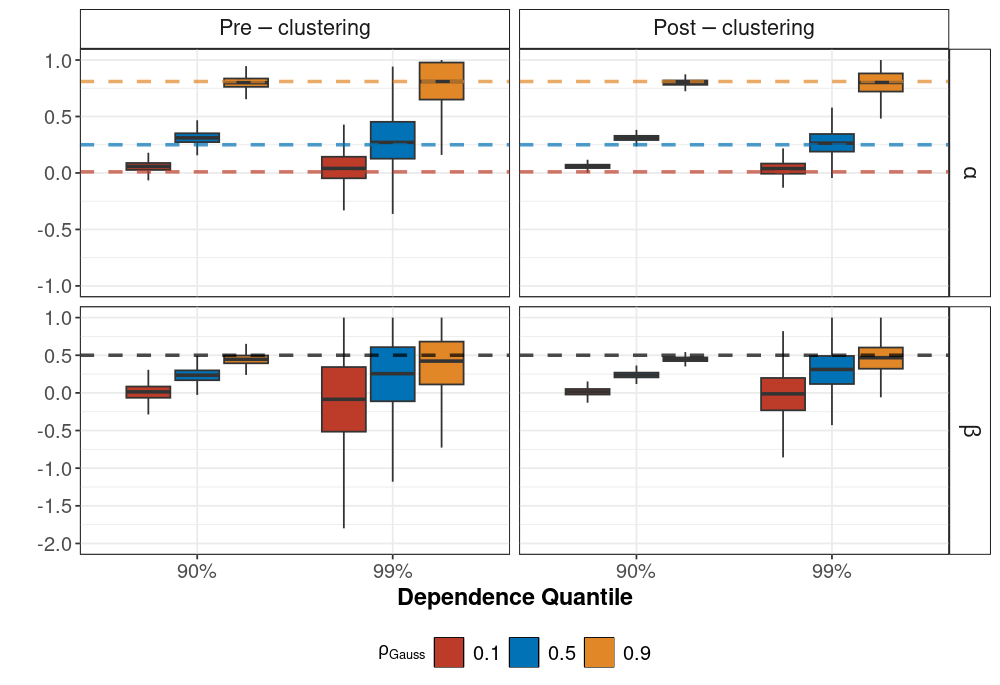
\includegraphics[width = 0.8\linewidth]{figure_1.png}
    \caption{\emph{ 
    Boxplots of estimates of $\alpha_{\mid i}$ (top) and $\beta_{\mid i}$ (bottom) for the conditional extremes model pre- and post-clustering with bivariate Gaussian data simulated at 12 sites, belonging equally to three known clusters. 
    The x-axis gives $q$, the level of the conditioning quantile used to fit the model, and the boxes are coloured by the true Gaussian copula correlation parameter, $\rho_{\text{Gauss}}^s$.
    The horizontal lines indicate the true theoretical values of $\alpha_{\mid i}$ and $\beta_{\mid i}$, with the colours for $\alpha_{\mid i}$ corresponding with the true $\rho_{\text{Gauss}}^s$ values.
    }}
   \label{fig:00_gauss_cop}
\end{figure}


\subsection{Mixture model setting}
\label{subsec:sim_mixture}

We extend our simulation design to mixtures of Gaussian and Student $t$-copulas \citep{Demarta2007-ap}, which induce asymptotic independence and asymptotic dependence, respectively, and whose dependence strength is determined by their respective correlation parameters $\rho_{\text{Gauss}}^s$ and $\rho_{\text{t}}^s \in [0, 1]$.

To obtain a sample of size $n = 1000$ from the mixture copula, at each site $s =1, \ldots, 12$, we combine $n/2 = 500$ samples from the Gaussian copula described in Section~\ref{subsec:sim_gauss} (with correlation parameter $\rhou{Gauss}^s$), and $n/2 = 500$ observations from a Student $t$-copula with 3 degrees of freedom and correlation $\rhou{t}^s$, before applying the Laplace transformation in Equation~\eqref{eq:laplace} to obtain the pairs $(Y_{1,s}, Y_{2,s})$ at site $s$.

In Section~\ref{subsubsec:sim_competing_methods}, we compare our method to the leading extremal competitor in the bivariate case \citep{Vignotto2021} and, in Section~\ref{subsubsec:sim_extension}, we show how our approach uniquely handles clustering of multivariate extremes in higher dimensions ($d > 2$).
Finally, Section~\ref{subsubsec:sim_realistic} considers a setting with $D = 60$ locations across three unequally sized clusters, and locations in the same cluster exhibiting perturbations in their correlation parameters.
Performance is evaluated using the ARI, with 500 replicated experiments per setting.

\subsubsection{Comparison to \citet{Vignotto2021}}
\label{subsubsec:sim_competing_methods}

When $d = 2$, we compare our extremal clustering method to that of \citet{Vignotto2021}.
We generate $n = 1000$ observations at $D = 12$ sites, using the mixture of Gaussian and t-copulas (with Laplace margins), as described above. 
Two clusters of sites $s = {1, \ldots, 6}$ and $s = {7, \ldots, 12}$ are defined with different values of $\rhou{t}^s$. 
We set $\rhou{t}^s = \rho_{\text{t}_1}$ for $s = 1, \ldots, 6$ and $\rhou{t}^s = \rho_{\text{t}_2}$ for $s = 7, \ldots, 12$, while $\rhou{Gauss}^s$ is the same for both clusters. 
We consider a range of extremal dependence scenarios defined over a grid of values $\left(\rhou{Gauss}^s \in \{0.1, 0.2, \ldots, 1.0\}, \rho_{\text{t}_1}^s \in \{0.1, 0.3, \ldots, 0.9\}, \rho_{\text{t}_2}^s \in \{0, 0.2, \ldots, 0.8\}\right)$.
We estimate the CE model using $q = 0.9$, and clusters were obtained using the aggregated dissimilarity matrix $M$ in Equation~\eqref{eq:aggregate_matrix}.

The results are shown in Figure~\ref{fig:01_ce_vs_vi}. 
Across the range of considered bivariate extremal dependence structures, our method consistently outperforms that of \citet{Vignotto2021}. 
Both methods have high ARI when the cluster-wise difference in $\rhou{t}^s$ is larger, since greater disparity naturally makes clusters more distinct and clustering easier. 
Both methods perform better when the Gaussian and t-copula correlations are higher.
This may be because the Gaussian copula becomes more similar to the t-copula for higher values of $\rhou{Gauss}$, thus allowing the clustering approach to focus on differences in the t-copula.

\begin{figure}[htb]
    \centering
    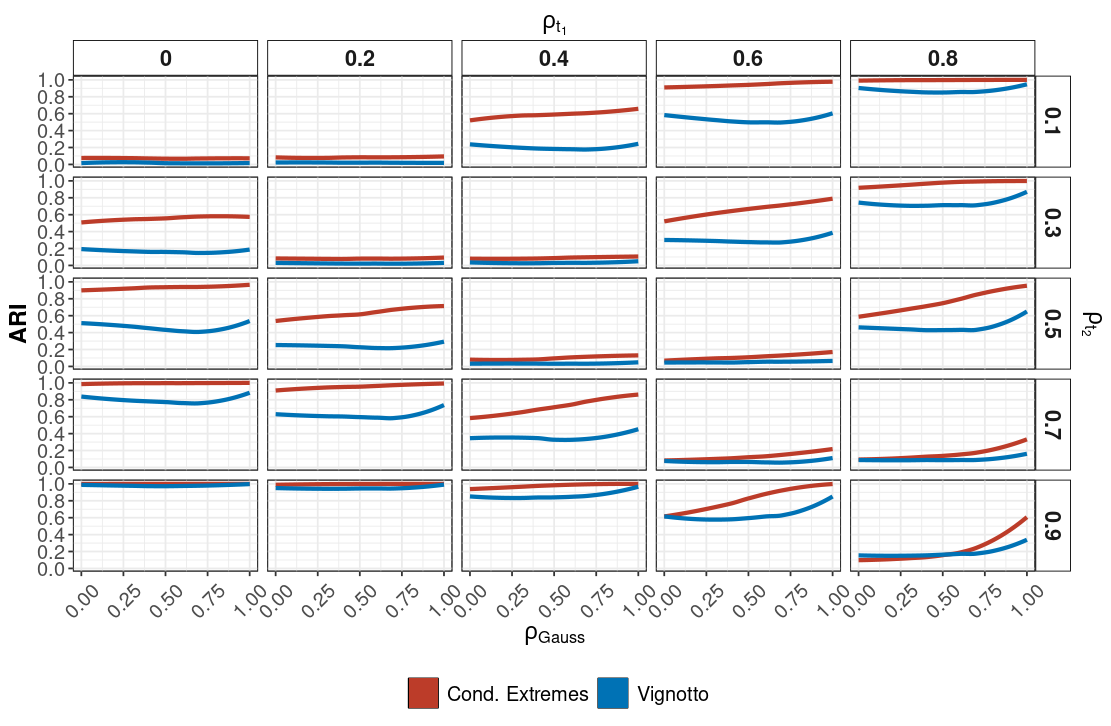
\includegraphics[width = 0.8\linewidth]{figure_2.png}
    \caption{\emph{
    Comparison of our conditional extremes-based approach and the method of \citet{Vignotto2021}.
    The x-axis represents the Gaussian correlation parameter $\rhou{Gauss}$, with facet labels indicating the t-copula correlation parameters, $\rho_{\text{t}_1}$ and $\rho_{\text{t}_2}$, for the two true clusters.
    The smoothed lines show the average ARI across bootstrap samples, for both methods, with smoothing performed using a generalised additive model.
    }}
    \label{fig:01_ce_vs_vi}
\end{figure}

\subsubsection{Extension to higher dimensions}
\label{subsubsec:sim_extension}

While the method of \citet{Vignotto2021} is restricted to $d = 2$ dimensions, our approach can be extended to $d \geq 3$ variables. 
To illustrate this, we extend the simulation study of Section~\ref{subsubsec:sim_competing_methods} by simulating at $D = 12$ locations, with two equally-sized clusters of sites each with $n = 1000$ observations per site, but now for $d = 3$ variables, using the same grid of ($\rhou{Gauss}, \rho_{\text{t}_1}, \rho_{\text{t}_2}$) values as in Section~\ref{subsubsec:sim_competing_methods}.
Our mixture copula now has three dimensions (with all pairwise correlations equal), and we fit three CE models at each site. 
Clustering is performed using the aggregated divergence matrix $M$ from Equation~\eqref{eq:aggregate_matrix}.
The results show that our proposed method performs well for $d =3$, with the same patterns in ARI emerging as in the bivariate case in Section~\ref{subsubsec:sim_competing_methods}.
In fact, performance is markedly stronger in three dimensions than in two. 
This is not surprising, as the CE fits in this setup are similar in both two and three dimensions, with the same $\rhou{t}^s$ being used across all variable pairs.
Therefore, the aggregated matrix $M$ in Equation~\eqref{eq:aggregate_matrix} is computed similarly, just averaged over more models with more data, which naturally improves clustering performance.

\begin{figure}[htb]
    \centering
    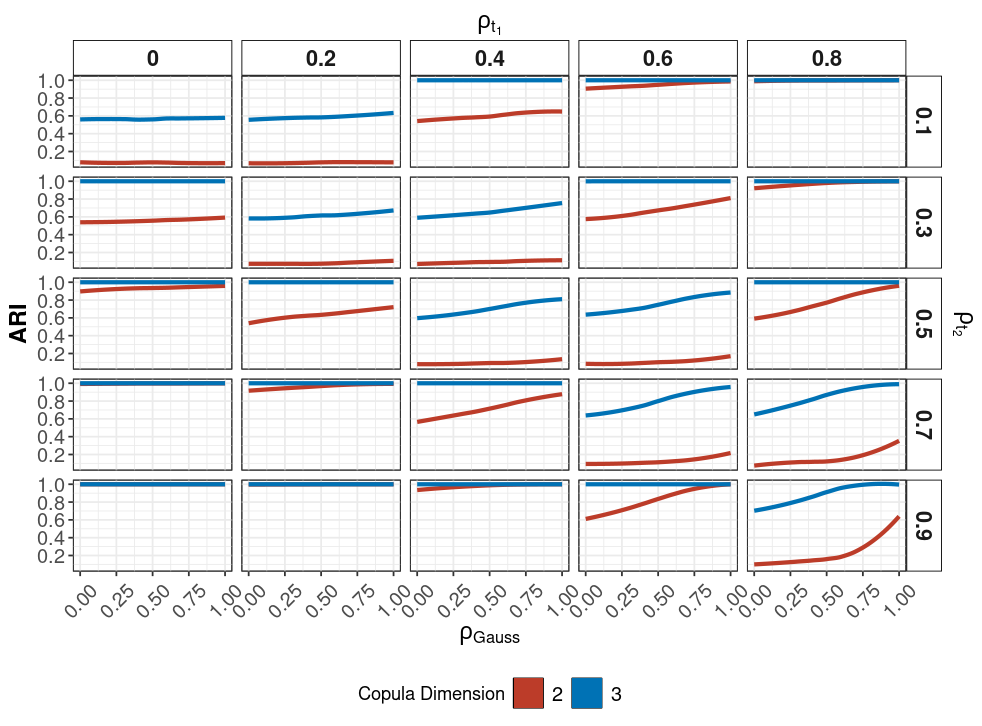
\includegraphics[width = 0.8\linewidth]{figure_3.png}
    \caption{\emph{
        Comparison of clustering performance for $d = 2$ and $d=3$ variables and two equally-sized clusters. 
        The x-axis represents the Gaussian correlation parameter $\rhou{Gauss}$ for both clusters, and the facet labels show the t-copula correlation parameters, $\rho_{\text{t}_1}$ and $\rho_{\text{t}_2}$, for the two true clusters.
        The smoothed lines show the average ARI across bootstrap samples, with smoothing performed using a generalised additive model.
    }}
   \label{fig:02_3d}
\end{figure}


% Expand to up to 5 dimensions!
To further illustrate the performance of our method in higher dimensions, we consider a specific case from the grid where $\rho_{\text{t}_1} = 0.4$ and $\rho_{\text{t}_2} = 0.5$. 
This setting presents a challenging clustering scenario in both two and three dimensions, as the cluster-wise difference in the t-copula correlation parameters is small. 
Figure~\ref{fig:02b_5d} displays the results when the dimensionality of the copula mixture is increased from $d = 2$ to $d = 5$, based on 500 simulations across all considered $\rhou{Gauss}$ values. 
Cluster accuracy improves steadily with dimension, reaching values close to 1 across all $\rhou{Gauss}$ settings when $d = 5$. 
These gains should be interpreted cautiously, since as mentioned above we use the same $\rhou{t}^s$ across all variable pairs, thus not altering the pairwise extremal dependence structure and instead increasing the amount of data as $d$ increases.
Having separate $\rhou{t}^s$ values for each variable pair would increase the complexity and signal-to-noise ratio of the clustering task, and likely reduce performance.
Nevertheless, the results demonstrate that the proposed method scales effectively to higher dimensions and performs well in multivariate settings. 

\begin{figure}[htb]
    \centering
    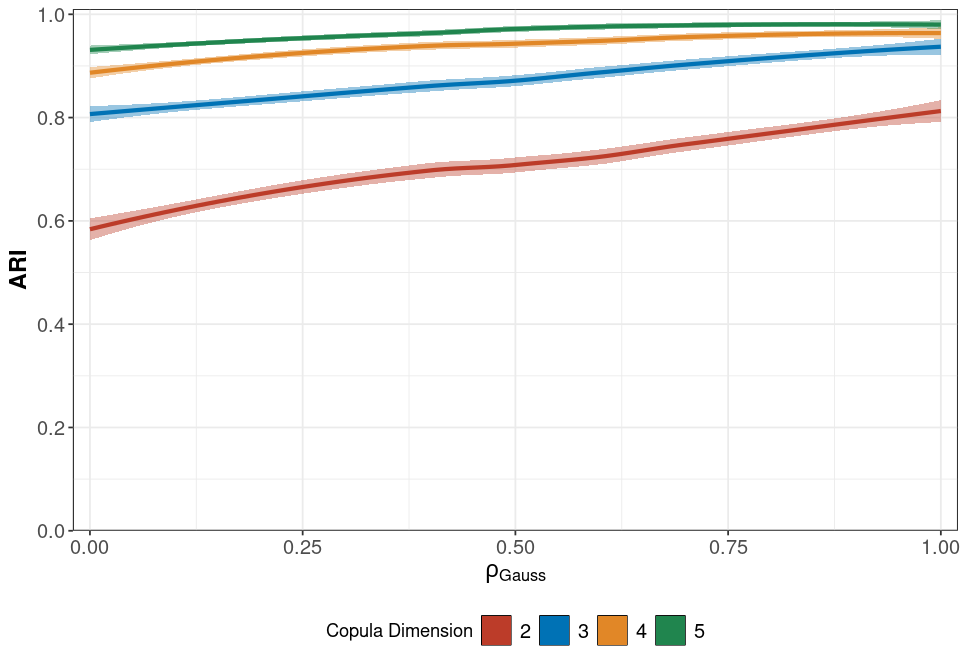
\includegraphics[width = 0.7\linewidth]{figure_4.png}
    \caption{\emph{
        Evaluation of clustering for $d = 2$ to $d = 5$ variables and two equally-sized clusters for simulations at 12 sites from a mixture of Gaussian and t-copulas.
    The t-copula correlation parameters for each true cluster were set to $\rho_{\text{t}_1} = 0.4$ and $\rho_{\text{t}_2} = 0.5$. 
A sequence of values are considered for the Gaussian correlation parameter $\rhou{Gauss}$, as represented on the x-axis.
    The smoothed lines show the average ARI and associated uncertainty across bootstrap samples, with smoothing performed using a generalised additive model.
}}
\label{fig:02b_5d}
\end{figure}

\subsubsection{Extension to more sites}
\label{subsubsec:sim_realistic}

We now design another simulation study to better mimic the structure of the Irish meteorological dataset, to be analysed in Section~\ref{sec:application}. 
Data are generated at $D = 60$ sites, each with $n = 1000$ observations of $d = 2$ variables, using the mixture of Gaussian and t-copulas.
The 60 sites are partitioned into three unequally-sized clusters of 10, 20, and 30 sites. 
At each location, the true $\rho_{\text{t}}^s$ is perturbed by adding $\text{Unif}(-0.05, 0.05)$ noise, making the clustering task more challenging.
We now have a separate t-copula correlation parameter for each of the three clusters, denoted by $\rho_{\text{t}_1}, \rho_{\text{t}_2}$, and $\rho_{\text{t}_3}$.
To reduce the dimensionality of the grid of considered copula parameter values, a constant $\rhou{Gauss} = 0.5$ is used across all sites and experiments. 

% results
The results of 500 repetitions of this simulation study are shown in Figure~\ref{fig:03_realistic}.
Similarly to the previous simulation studies, our clustering method performs well, particularly when the differences in t-copula correlation parameters between clusters are larger. 
For example, the best performance is observed where $\rho_{\text{t}_1} = 0.9, \rho_{\text{t}_2} = 0.1$, and $\rho_{\text{t}_3} = 0.5$, as the clusters are most distinct, while conversely, performance is worst for $\rho_{\text{t}_1} = 0.6, \rho_{\text{t}_2} = 0.4$, and $\rho_{\text{t}_3} = 0.5$. % \todo{Include this to aid reading of figure, is it necessary?}

\begin{figure}[htb]
    \centering
    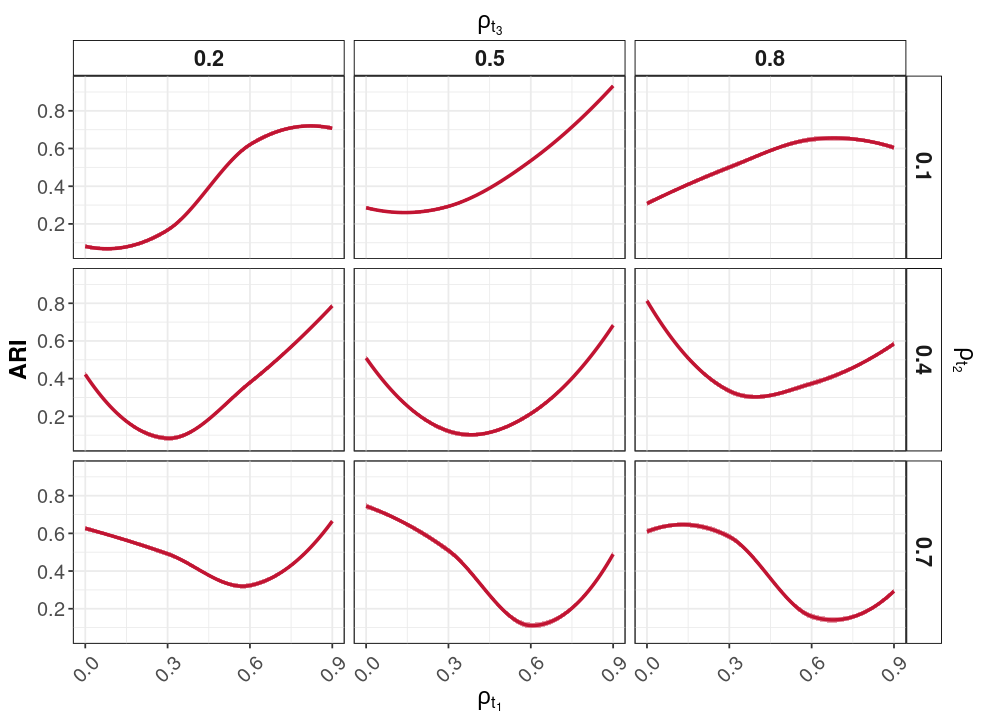
\includegraphics[width = 0.7\linewidth]{figure_5.png}
    \caption{\emph{Evaluation of clustering performance for $d = 2$ variables and three clusters of 60 locations for simulations from a mixture of Gaussian and t-copulas.
        The true x-axis and facet labels show the t-copula correlation parameters,  $\rho_{\text{t}_1}, \rho_{\text{t}_2}$, and $\rho_{\text{t}_3}$, for each of the three true clusters, for a Gaussian copula correlation of $\rhou{Gauss} = 0.5$. 
    The smoothed lines show the average ARI across bootstrap samples, with smoothing performed using a generalised additive model. 
    }}
   \label{fig:03_realistic}
\end{figure}

\section{Application to Irish meteorological data}
\label{sec:application}
% Section Intro
We now apply our extremal clustering method to meteorological observations from the Republic of Ireland. 
In Section~\ref{subsec:app_data}, we describe the precipitation and wind speed measurements used in our analysis and present exploratory analysis (using the $\chi$ statistic from Equation~\eqref{eq:chi}) on the extremal dependence between the two variables. 
In Section~\ref{subsec:app_ce}, we discuss fits of the conditional extremes (CE) model, and, in Section~\ref{subsec:app_clust}, we apply our extremal clustering approach. 

\subsection{Ireland meteorological data}
\label{subsec:app_data}

\begin{figure}[htb]
    \centering
    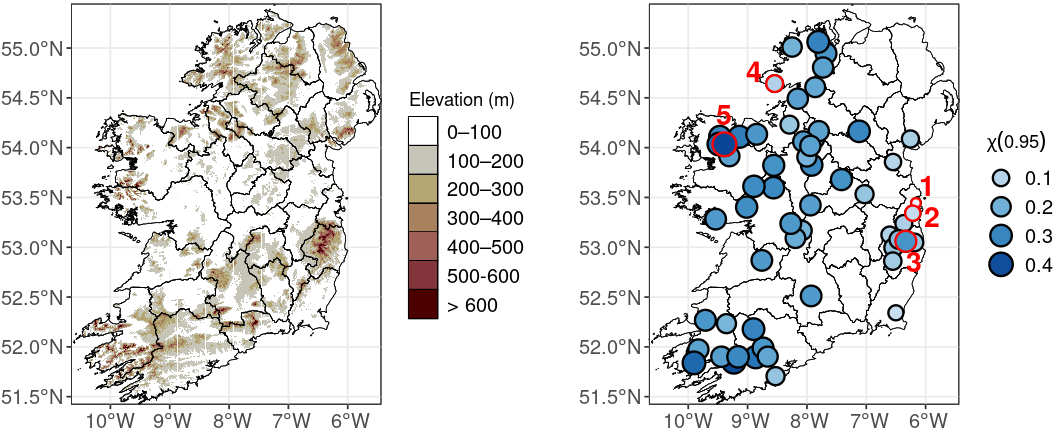
\includegraphics[width = 0.8\linewidth]{figure_6.png}
    \caption{\emph{
    Left: elevation (m) profile of Ireland.
    Right: Estimated $\chi(0.95)$ between precipitation and wind speed at all 59 locations. Darker colours and larger points indicate stronger asymptotic dependence.
    Locations in red are (1) Malahide Castle, Dublin, (2) Ringsend, Dublin, (3) Glenmacnass, Wicklow, (4) Kilcar, Donegal, and (5) Derryhillagh, Mayo.
}}
   \label{fig:chi}
\end{figure}

We analyse the joint extremal behaviour of precipitation and wind speed at $D=59$ sites across the Republic of Ireland from 1990 to 2020, inclusive. 
Precipitation and wind speed data are obtained from the Met Éireann archive \citep{metHistoricalData}, and ERA5 Reanalysis \citep{Hersbach2020}, respectively. 
Met Éireann data are irregularly spaced over space, while ERA5 provides spatial averages on a regular $0.25^{\circ} \times 0.25^{\circ}$ grid.
We match each spatial site to the grid cell in which it lies. 
The dataset spans 11,323 consecutive daily observations.

% Preprocessing
We focus on the winter months, October to March, following \citet{Vignotto2021}.
Precipitation are aggregated into weekly sums, and daily wind speed maxima are aggregated into weekly averages.
This weekly temporal scale reflects the typical lag between extreme precipitation and wind speed during storm events \citep{Bengtsson2009}, and reduces short-term temporal dependence not accounted for in our model. 
Weeks with no precipitation are excluded, resulting in 5,022 observations across all $D = 59$ sites. 

% Chi statistic
We explore the extremal dependence structure of the data using the $\chi$ statistic introduced in Equation~\eqref{eq:chi}.
Figure~\ref{fig:chi} shows empirical estimates of $\chi(0.95)$ at all 59 sites.
An elevation profile of Ireland is also shown in Figure~\ref{fig:chi}, which may help further explain some of this spatial structure.
Non-zero values are observed at almost all sites, indicating positive extremal dependence between precipitation and wind speed. 
In practical terms, this suggests that extreme wind speeds tend to be accompanied by high precipitation, and vice versa. 
A clear spatial pattern emerges: extremal dependence is strongest in the south west, with the highest values along the Atlantic coast, notably in counties Kerry, Galway, Mayo, and Donegal, and weaker along the east coast, in Dublin, Wexford, and Louth. 
The highest $\chi(0.95)$ value (0.414) is observed at Derryhillagh in Mayo (Figure~\ref{fig:chi}, location (5)), while the lowest (0.0005) is at Malahide Castle in Dublin (Figure~\ref{fig:chi}, location (1); hereafter `Malahide').

Some spatial outliers are also apparent. 
Kilcar in Donegal (Figure~\ref{fig:chi}, location (4)) has a relatively low $\chi(0.95)$ value (0.109), despite its west-coast location, while some sites in county Wicklow show unusually high values for the east, particularly Glenmacnass (Figure~\ref{fig:chi}, location (3); 0.268).
The latter may be related to the influence of the Wicklow Mountains, as reflected in the elevation profile (Figure~\ref{fig:chi}). 
It may be of interest to investigate if these outliers in $\chi(0.95)$ are reflected in the CE model parameter estimates, and whether clustering can identify them.
These results indicate distinct regional patterns of extremal dependence, as well as notable outliers, motivating the use of our extremal clustering framework to characterise and interpret this spatial structure more formally. 

\subsection{Conditional extremes estimates}
\label{subsec:app_ce}

% Procedure and results pre-clustering (choice of quantile)
We transform the precipitation and wind speed data, separately at each location, to Laplace margins, with the empirical rank transform replacing $F_{X_i}$ in Equation~\eqref{eq:laplace}.
To select an appropriate quantile level $q$ for fitting the CE model (see Section~\ref{subsec:ce_model}), we estimate the parameters $(\alpha_{\mid i}, \beta_{\mid i})$ at a sequence of levels $q$, to identify the lowest $q$ beyond which parameter estimates appear stable.
Estimates are generally stable for both models, i.e.,\@ precipitation conditional on wind speed and vice versa, down to $q = 0.85$, with similar maximum likelihood estimates across 500 bootstrap samples for $(\alpha_{\mid i}, \beta_{\mid i})$.
Threshold stability plots for the CE fits at the five locations highlighted in Figure~\ref{fig:chi} are included in Figures~\ref{fig:boot_quantiles_malahide} -- \ref{fig:boot_quantiles_derryhillagh} of the supplementary materials.
Therefore, we fix $q = 0.85$ for the subsequent analysis.
In Figure~\ref{fig:clust_sens}, we show that our estimated extremal clustering is robust to the choice of $q$, with estimates shown for $q = 0.85, 0.88$, and $0.90$.

The estimated site-wise CE parameters are shown in Figure~\ref{fig:a_b_vals}.
Although interpretation is challenging due to variability in the estimates, as with the $\chi(0.95)$ estimates (Figure~\ref{fig:chi}), we observe some evidence of increasing $\alpha_{\mid i}$ values for both variables towards the west and south.
To mitigate uncertainty and aid interpretation, we cluster the locations using our extremal clustering approach. 

\begin{figure}[htb]
    \centering
    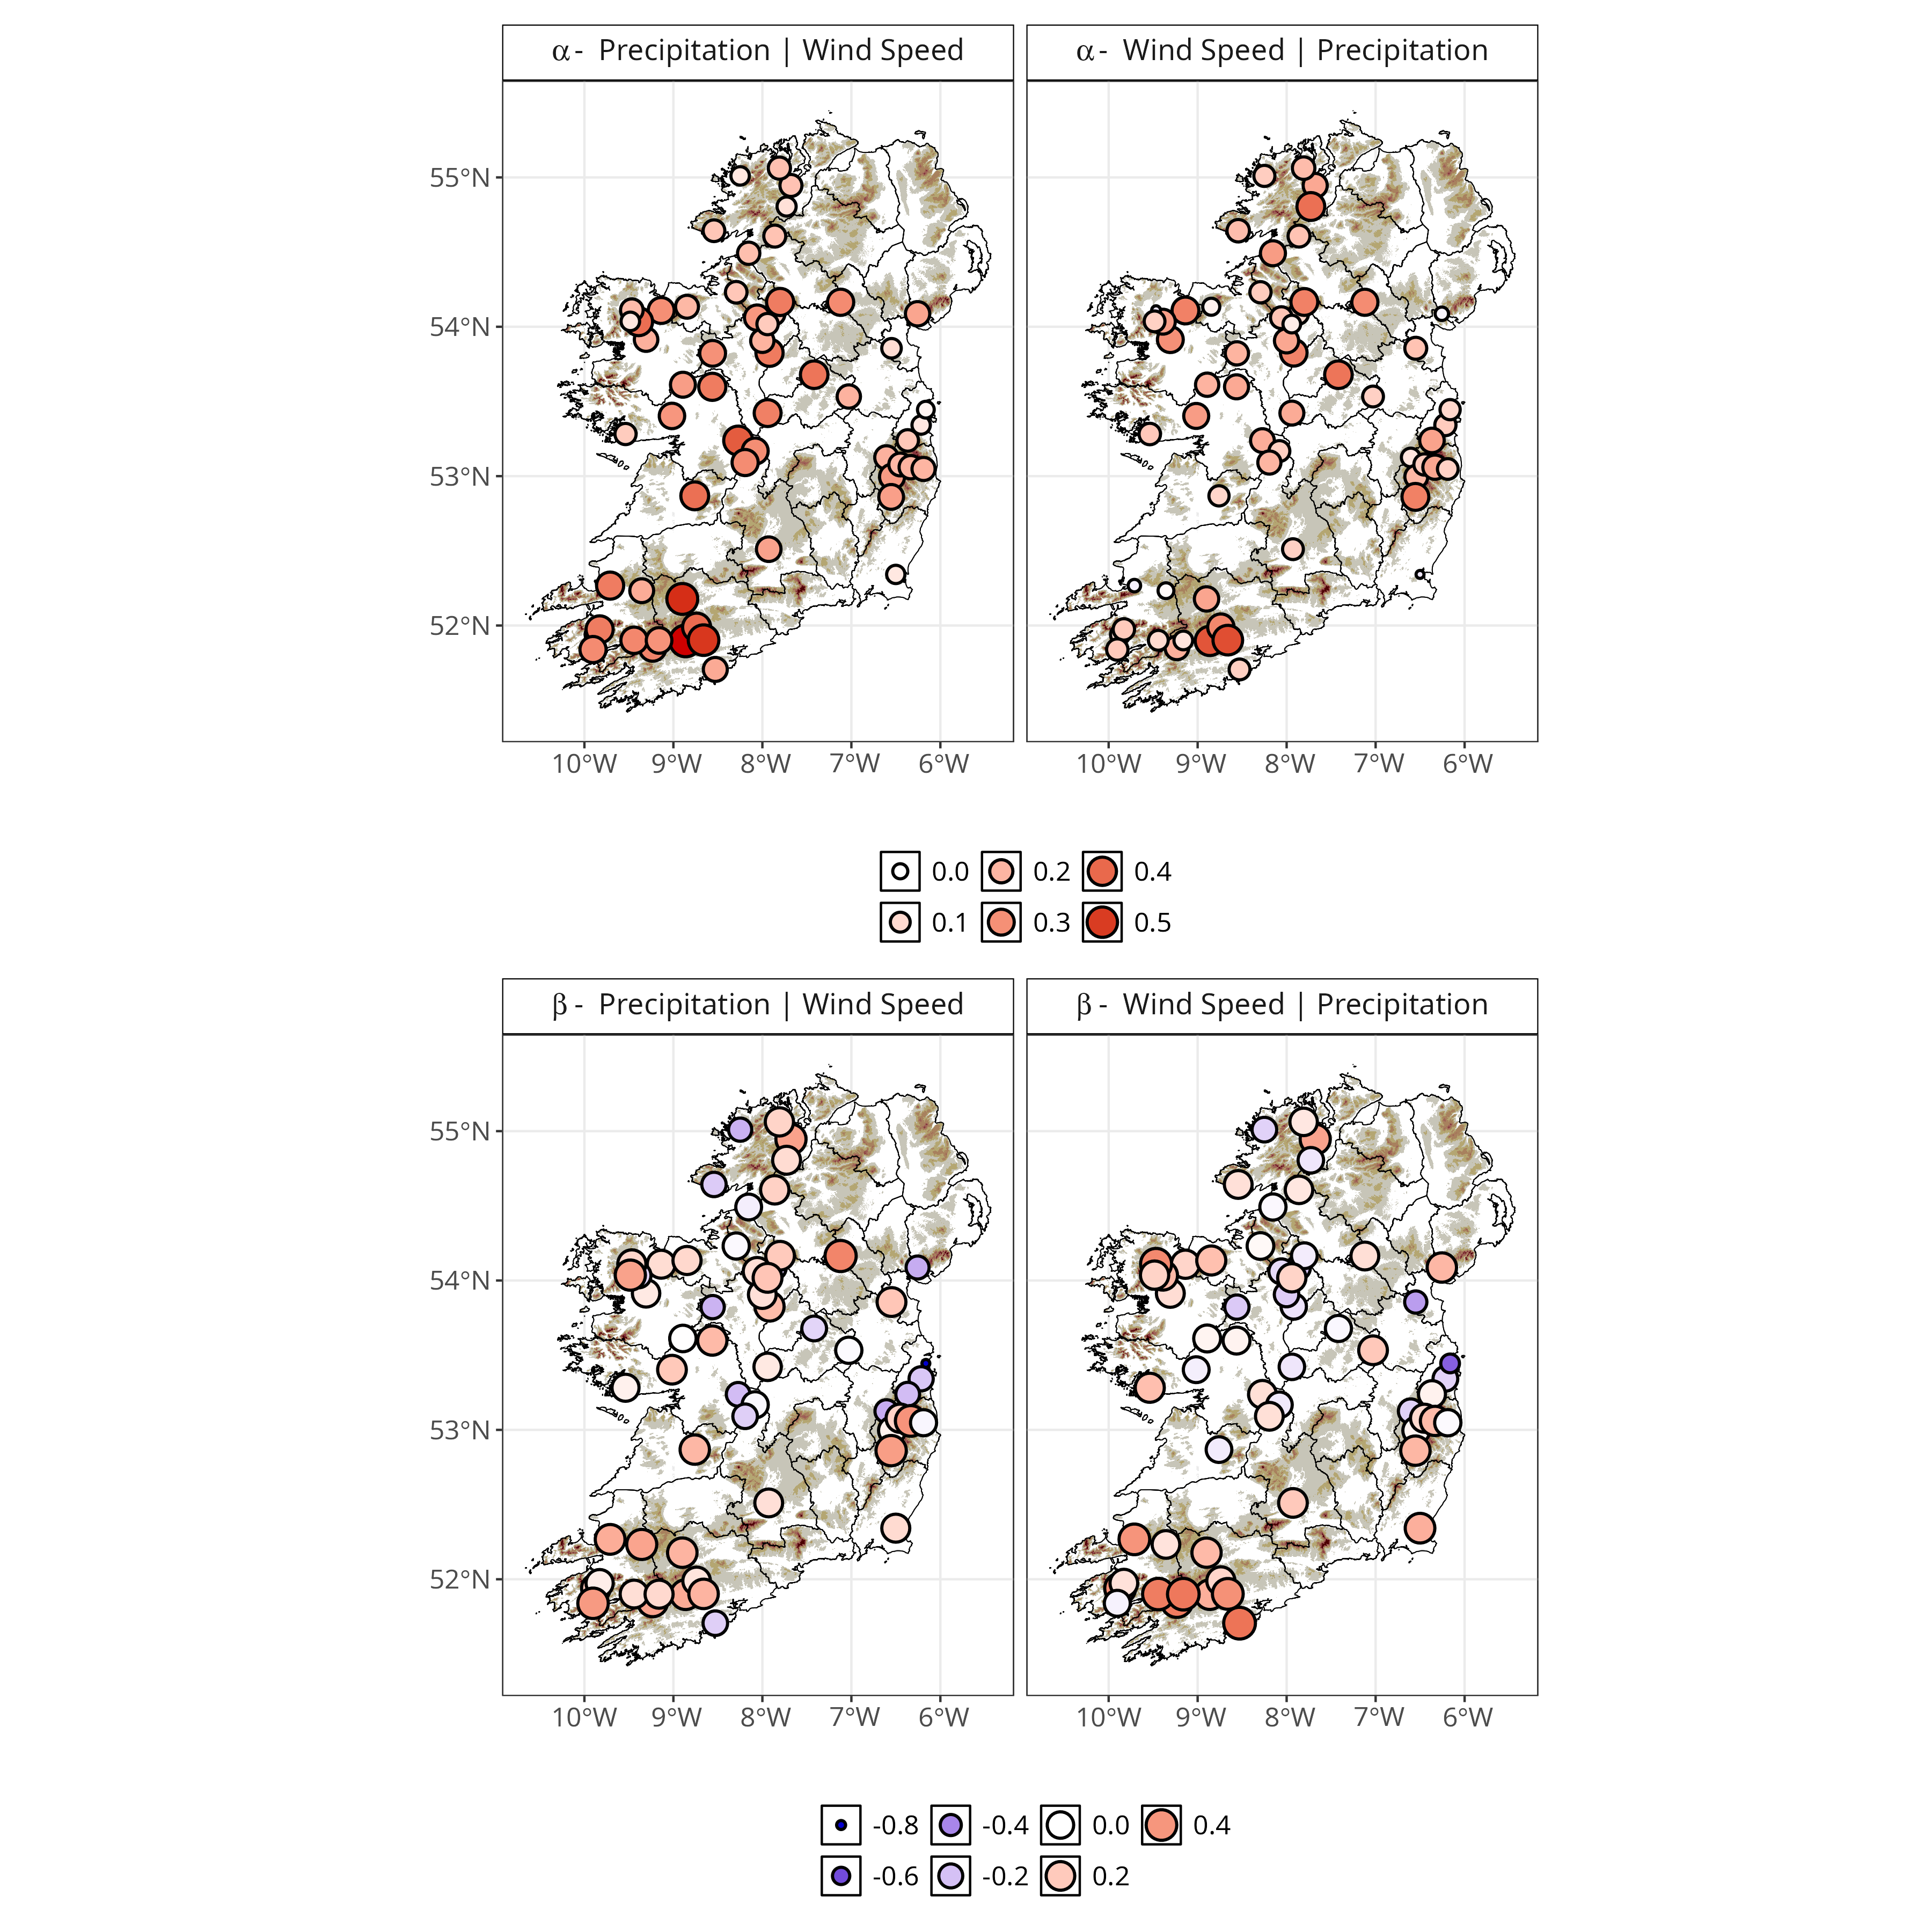
\includegraphics[width = 0.8\linewidth]{figure_7.png}
    \caption{\emph{
        Maps of site-wise estimated model parameters $\alpha_{\mid i, s}$ (top) and $\beta_{\mid i, s}$ (bottom) for precipitation conditional on wind speed (left) and wind speed conditional on precipitation (right).
        The colour scale is the same for both variables, with darker red and larger points indicating larger positive values of $\alpha$ and $\beta$, and darker blue and smaller points indicating smaller negative values.
   }}
   \label{fig:a_b_vals}
\end{figure}


\subsection{Clustering}
\label{subsec:app_clust}

We cluster the locations using the aggregated dissimilarity matrix $M$ as defined in Equation~\eqref{eq:aggregate_matrix}, and separately for each individual matrix $M^{(i)}, i = 1, 2$, as in Equation~\eqref{eq:distance_matrix}.
The number of clusters $k$ is chosen via the method in Section~\ref{subsec:clustering}, using the elbow plot of the $\mathrm{TWGSS}$. 
For all three clustering scenarios, clear elbows are observed at $k = 3$.
The elbow plots are provided in Figure~\ref{fig:elbow_plots} of the supplementary materials. 

The resulting cluster estimates are displayed in Figure~\ref{fig:clust_sol}.  
Across all three choices of dissimilarity matrix, the estimated clusters are broadly consistent, with three spatially distinct groups emerging.  
This spatial coherence is notable given that no explicit spatial information was used in model fitting or in the clustering, suggesting that the CE model parameters capture meaningful spatial structure in the extremal dependence of the data. 

When interpreting the clusters, we observe a clear contrast between the east and west coasts, separated by a central cluster.  
For precipitation conditional on wind speed, the clustering is somewhat less distinct, with the central cluster extending more extensively into parts of Galway, Mayo, and Donegal on the west coast.  
There are also notable outliers in the clusters, which we further discuss below. 

\begin{figure}[htb]
    \centering
    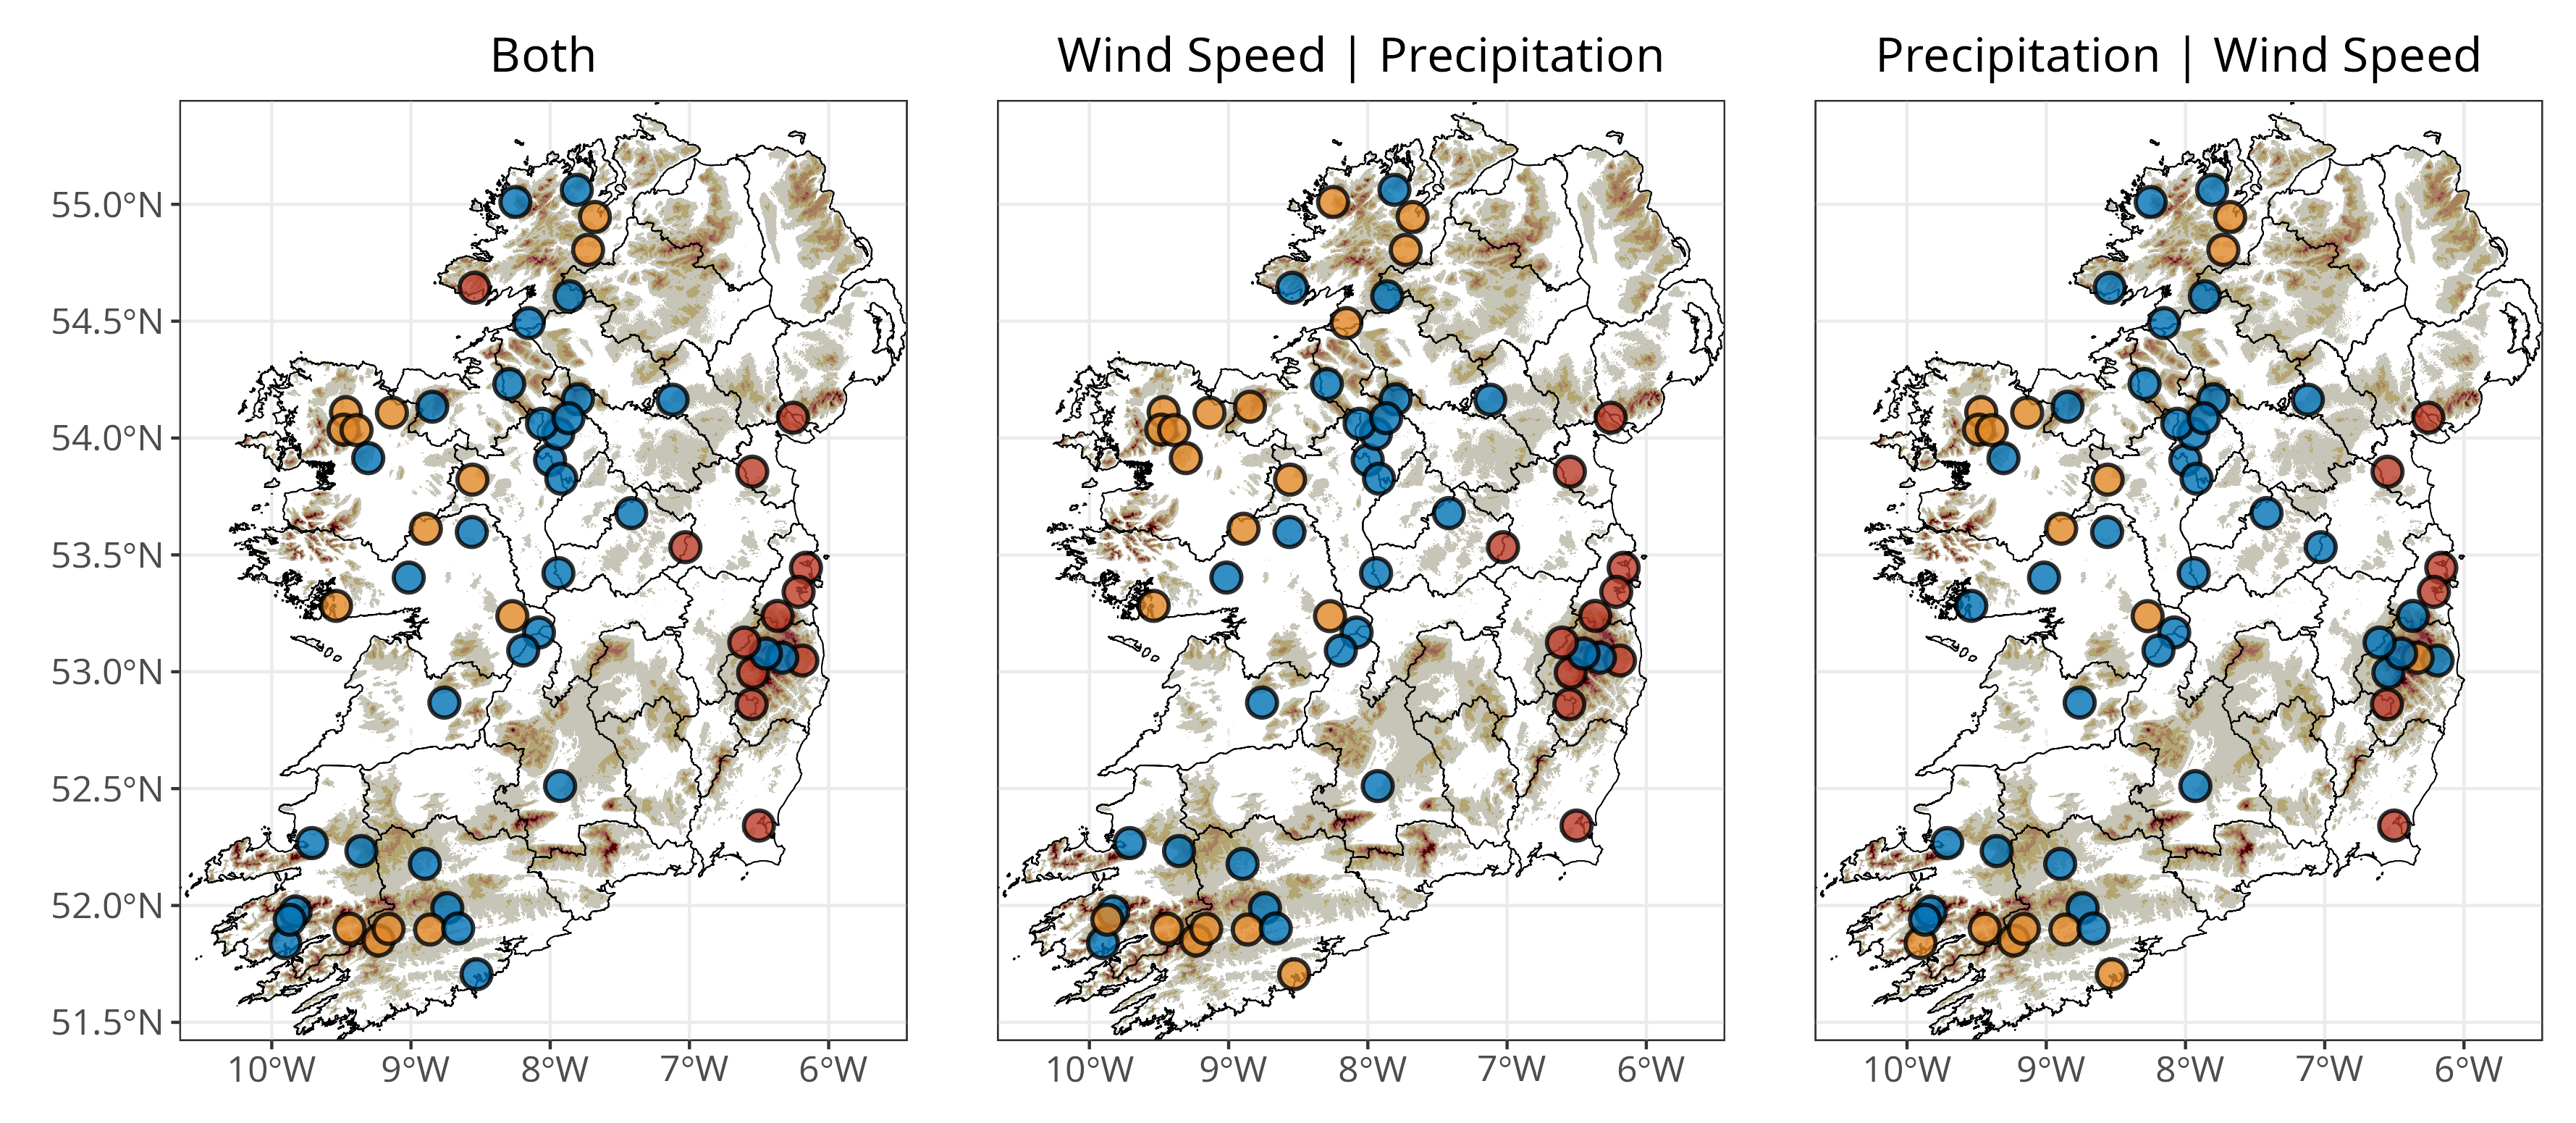
\includegraphics[width = 0.8\linewidth]{figure_8.png}
    \caption{\emph{
    Extremal cluster estimates using the dissimilarity matrix for wind speed conditional on precipitation (centre), precipitation conditional on wind speed (right), and the combined dissimilarity matrix (left). 
    Sites are coloured by cluster label.
}}
\label{fig:clust_sol}
\end{figure}

\begin{figure}[htb]
    \centering
    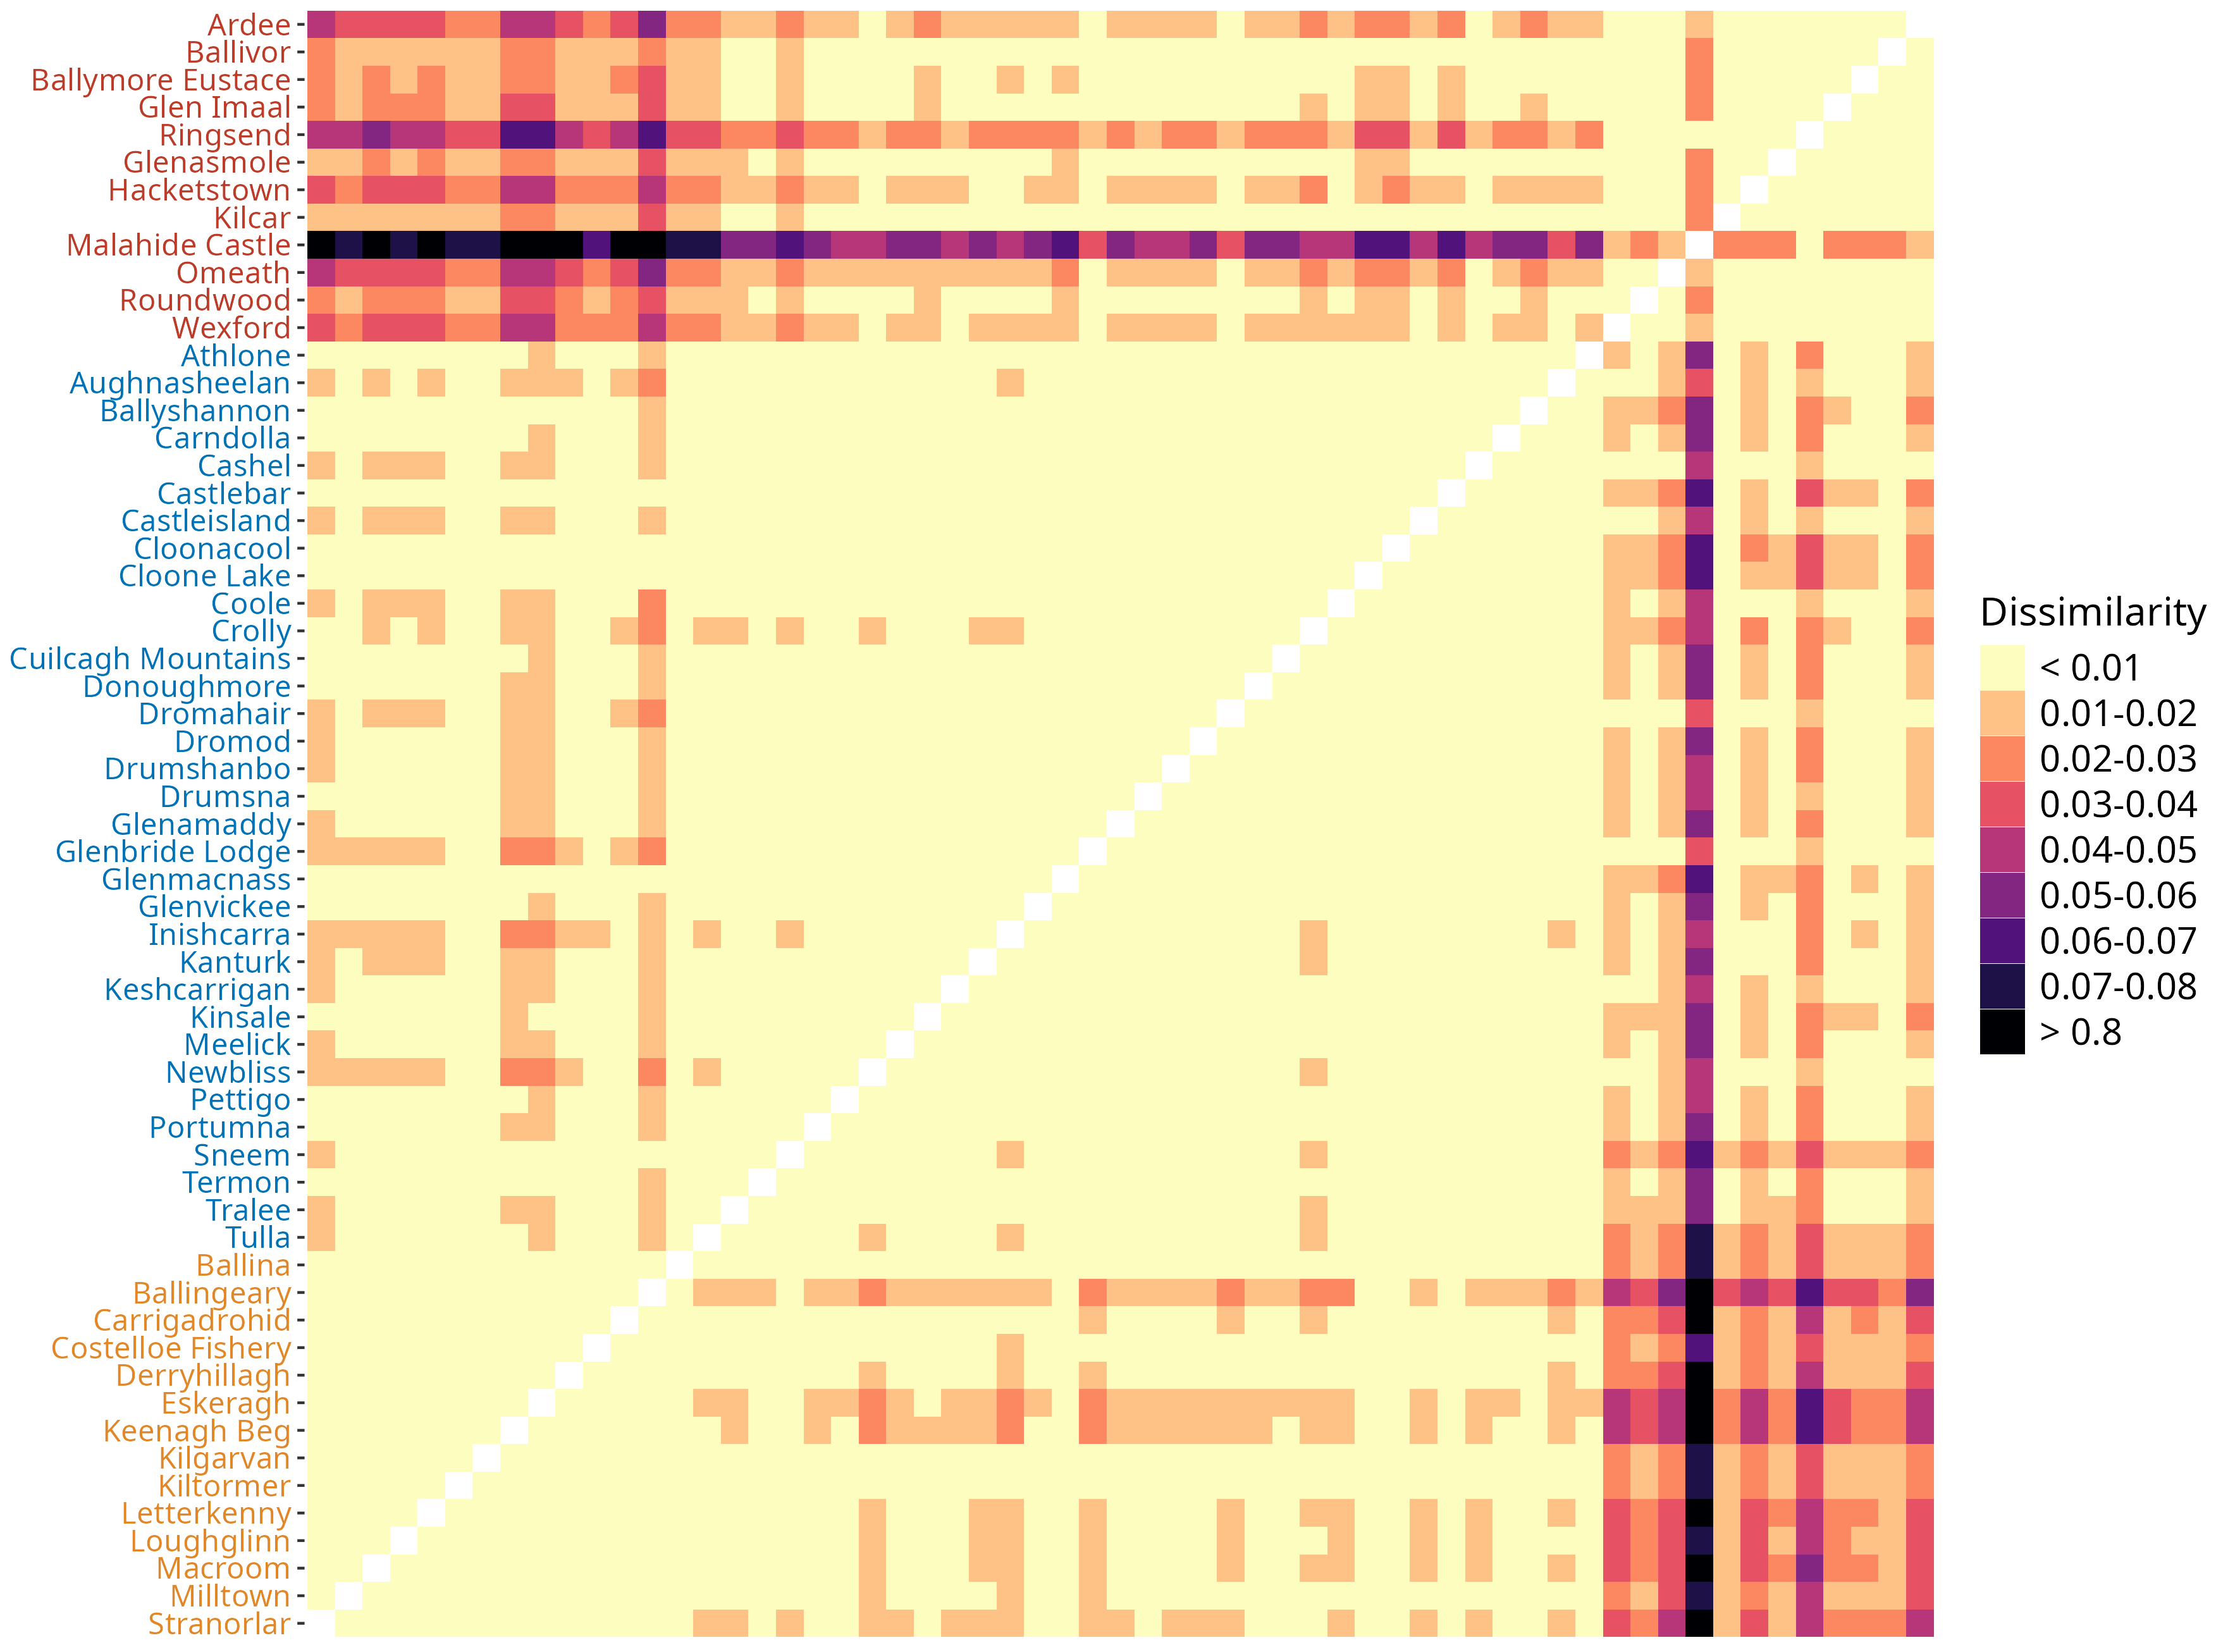
\includegraphics[width = 1.0\linewidth]{figure_9.png}
    \caption{\emph{
    Heatmap of the estimated aggregated dissimilarity matrix $M$.
The names of each site are coloured and ordered according to their estimated cluster labels, matching that of Figure \ref{fig:clust_sol}. 
The dissimilarity colour scale is shown on the right, with darker colours indicating larger values.
}}
\label{fig:dist_heatmap}
\end{figure}

% Analysis of dissimilarity matrix
In Figure~\ref{fig:dist_heatmap}, we visualise the dissimilarity matrix for the aggregated clusters (see left panel of Figure~\ref{fig:clust_sol}).
The clusters are quite distinct, with the dissimilarity between clusters being much larger than within-cluster dissimilarity, which rarely exceeds 0.01.
In particular, the difference between the eastern and western clusters is quite pronounced, with the intermediate central cluster acting as somewhat of a `buffer' between the two.
In contrast, the western and central clusters seem to be quite close, in that we observe many small inter-cluster pairwise dissimilarities between them. 
This indicates that allocation between the two is not always clear-cut and for several sites is nearly interchangeable, as observed in  the variable-specific estimated clusters in Figure~\ref{fig:clust_sol} and in the quantile sensitivity analysis in Figure~\ref{fig:clust_sens}, where membership between the two often switches. 
Also, if we only fit two clusters, we find that most of the central cluster members are assigned to the western cluster, reflecting this less obvious separation between the two compared to the more markedly different eastern cluster. 
A noticeable outlier in the dissimilarity matrix is Malahide, which we previously identified as having the lowest $\chi(0.95)$ value  in Figure~\ref{fig:chi}. 
Even within its own cluster, Malahide shows a relatively high dissimilarity to the other sites. 
Indeed, if we set $k=4$, Malahide becomes its own cluster (clustering results for $k=2$ and $k=4$ are provided in Figure~\ref{fig:cluster_dqu_k_2_4} of the supplementary materials).
Malahide also has the lowest mean weekly precipitation of any site; the second lowest is Ringsend, also in county Dublin (Figure~\ref{fig:chi} location (2)), which is the site closest to Malahide in terms of our dissimilarity measure. 
Finally, Malahide has very low $\chi(0.95)$ (Figure~\ref{fig:chi}) and $\alpha_{\mid i}$ (Figure~\ref{fig:a_b_vals}) estimates. 
Together, this may explain why we observe such outlying behaviour for Malahide.
Finally, Kilcar in County Donegal is the member of the eastern cluster with the smallest dissimilarity to the western cluster members.
This may reflect its geographic location in northwest Ireland, despite it's low $\chi(0.95)$ value (Figure~\ref{fig:chi}) relative to other west-coast sites.

\begin{figure}[htb]
    \centering
    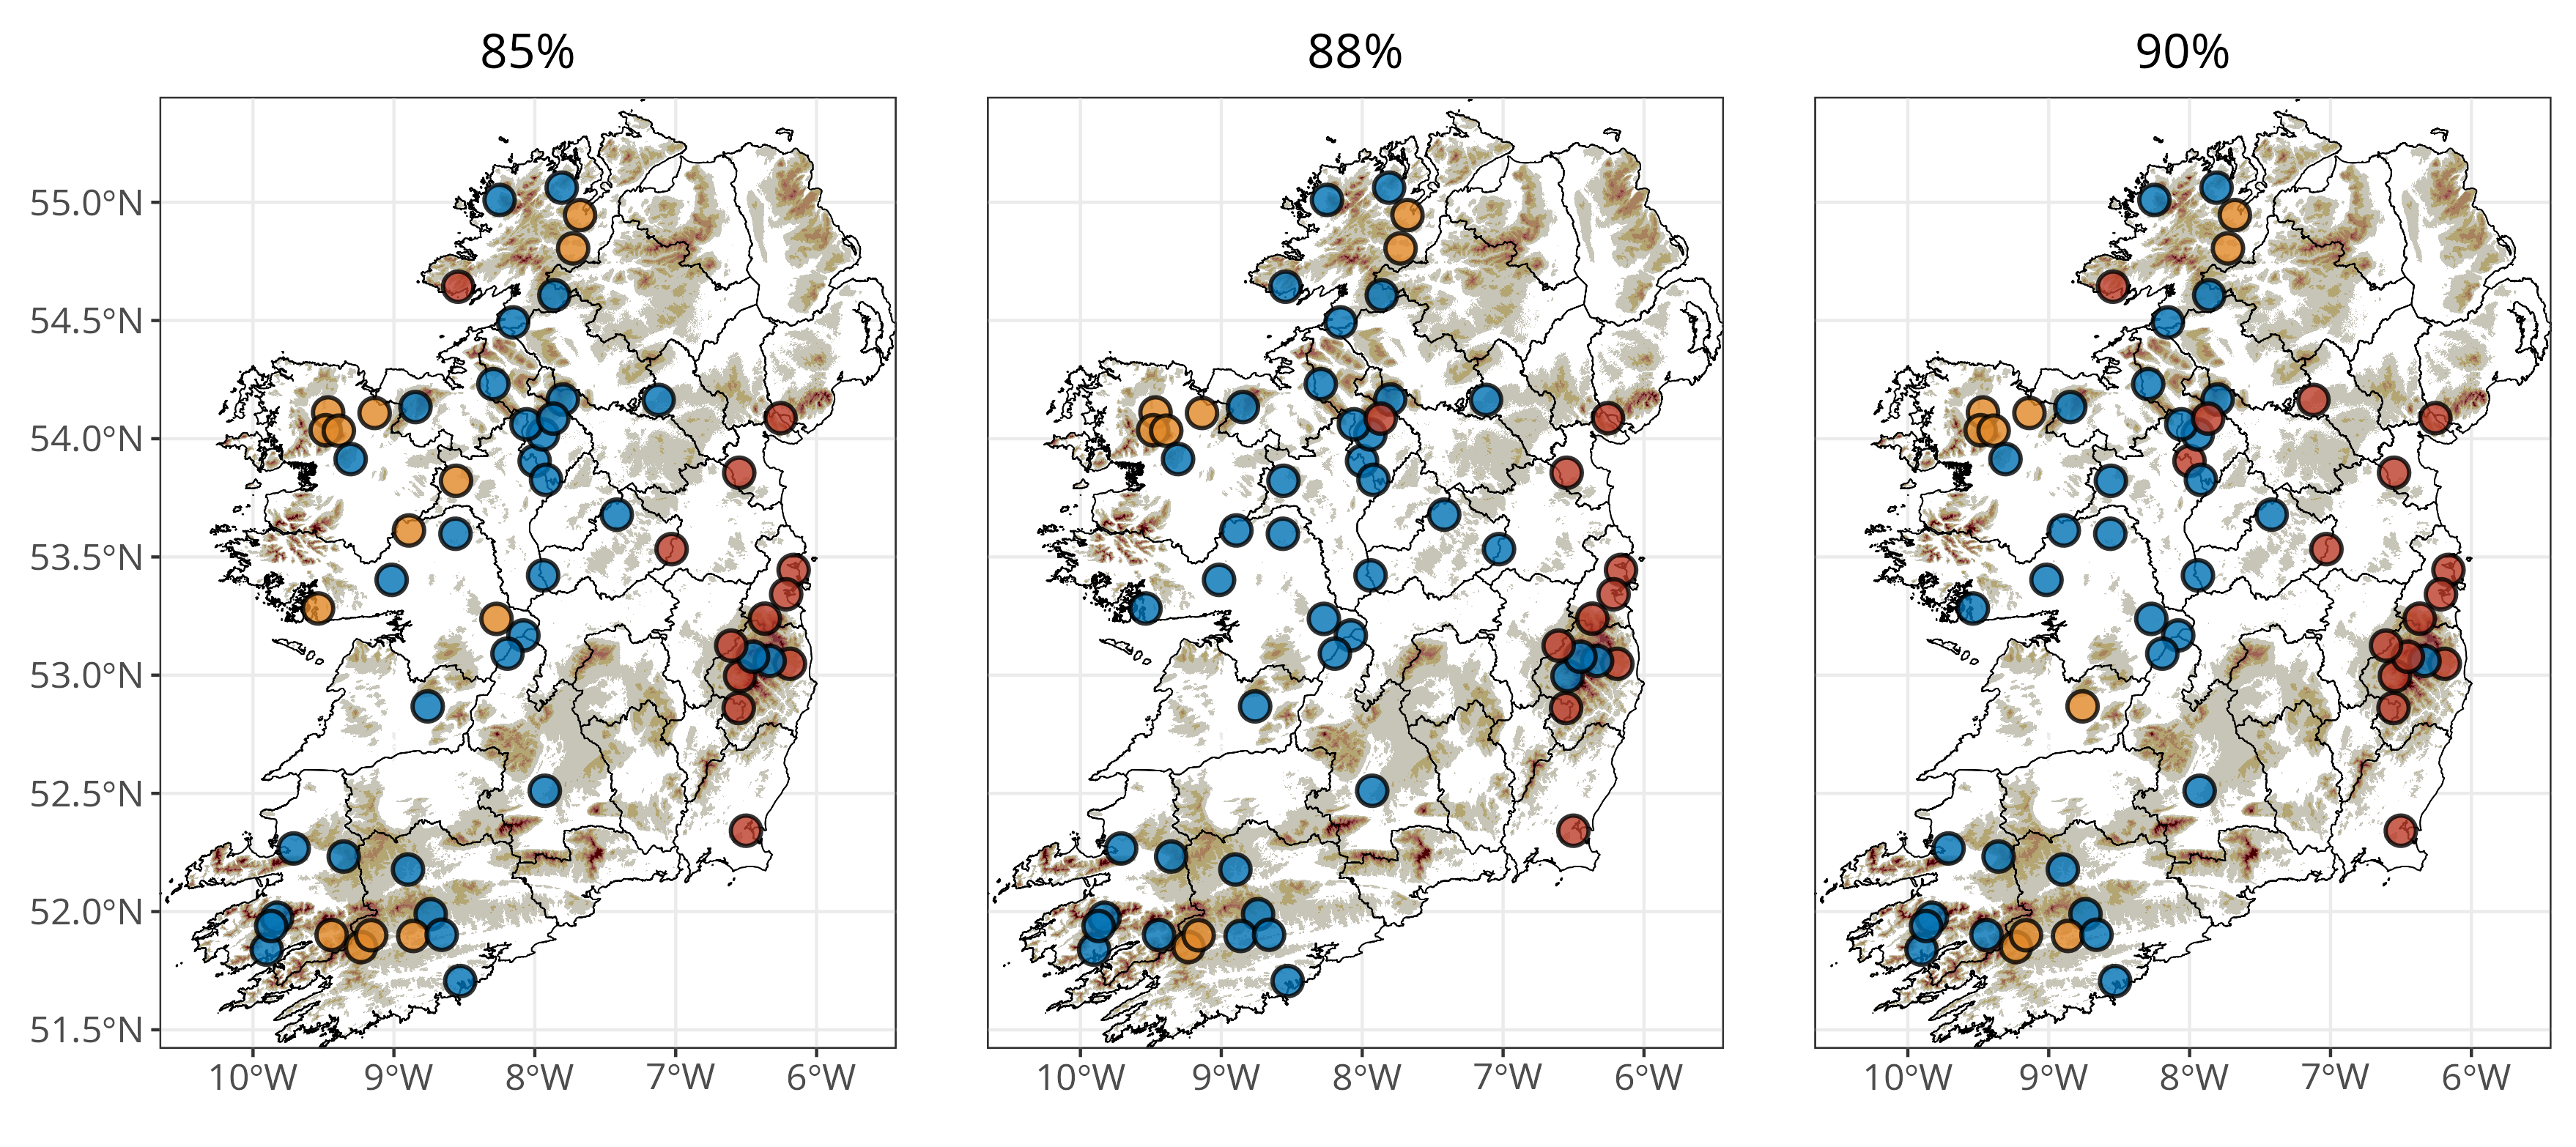
\includegraphics[width = 0.85\linewidth]{figure_10.png}
    \caption{\emph{
    Estimated extremal clusters with the conditional extremes model parameters estimated at $q = 0.85, q = 0.88$ and $q = 0.9$ quantiles, using the aggregated dissimilarity matrix. 
    Sites are coloured by cluster label. 
}}
\label{fig:clust_sens}
\end{figure}


% Sensitivity Analysis (to choice of DQU)
We perform a sensitivity analysis of the estimated clusters (with the aggregated dissimilarity matrix) to the choice of quantile level $q \in \{0.85, 0.88, 0.90\}$, in Figure~\ref{fig:clust_sens}.
The estimated clusters are similar across the three values of $q$, with some small differences. 
Noticeably, the earlier identified outlier at Kilcar in county Donegal is assigned to the eastern cluster when $q = 0.85$ and $q = 0.90$, but to the central cluster when $q = 0.88$.
Also, there are more sites in the western cluster when $q = 0.85$, with some sites moving to the central cluster for $q = 0.88$.
Interestingly, some of these sites then move back to the western cluster for $q = 0.90$.
Apart from these observations, the estimated clusters are generally quite similar across the three quantile levels, and so we conclude that our clustering method is relatively robust to the choice of quantile level.

\section{Discussion}
\label{sec:discuss}

% Quick summary
In this paper, we introduced a novel method for clustering multivariate extremes.
We proposed the expected conditional $\JSGa{}$ divergence \citep{Nielsen2019} as a measure of dissimilarity between multivariate conditional extremes (CE) models \citep{Heffernan2004}.
We leveraged the commonly-applied working Gaussian assumption to derive a closed-form expression for the $\JSGa{}$ divergence.
Efficient k-medoids clustering was then performed on the dissimilarity matrix derived from this measure. 
In our simulation study, a bivariate Gaussian copula example illustrated that our clustering method reduces parameter uncertainty and bias when the CE model is re-fitted with data pooled post-clustering.
Using mixtures of Gaussian and $t$-copulas, we showed that our method outperforms the method of \citet{Vignotto2021} across a range of bivariate extremal dependence scenarios.
Our method was also shown to be uniquely extendable to $d > 2$ dimensions. 
We applied our extremal clustering method to Irish meteorological data, consisting of 59 locations with weekly rainfall and wind speed observations.
Without explicitly incorporating spatial information, three clusters with distinct spatial patterns were identified, with well separated clusters representing the east and west coasts and the centre of Ireland.

% Extension
While we focused on a spatial application in this work, our method is more generally applicable to any setting where clustering of multivariate extremal dependence is desired.
For instance, it could be applied to clinical trial or public health data to cluster patients based on the tail dependence structure of their symptoms or biomarker measurements.
A neuroscience application was explored in \citet{Talento2025}, where the CE framework was used to highlight differences in the tail dependence of electroencephalogram (EEG) signals for seizure-prone and seizure-absent subjects. 
However, they used pre-defined clusters. Hence, we may expect our approach to be useful in similar applications, to identify subjects who have undergone extreme brain events, e.g., seizures.
In financial applications, we could cluster time periods according to the extremal dependence of log-returns of different assets, offering potential insights for portfolio management and risk assessment.

% Limitations: Gaussian assumption
While the residual Gaussian assumption on which our method relies may not hold for all datasets, our clustering approach showed good performance for all settings in Section~\ref{sec:sim}.
A possible alternative is to employ the generalised and asymmetric multivariate Gaussian distribution used in \citet{Farrell2025}. 
While this does not permit a closed-form divergence, our extremal clustering method could still be used, with costly numerical techniques used to estimate the dissimilarity matrix.
Indeed, if choosing to forgo this Gaussian assumption, it may be preferable to use the standard Jensen-Shannon divergence in place of the $\JSGa{}$ divergence, since the former is bounded \citep{Thiagarajan2025}.

% Limitations: Uncertainty
Another important limitation of our method is in its treatment of uncertainty.
We do not propagate uncertainty in the CE model estimates through to the clustering. 
To account for this, one possible approach is to use the bootstrap method of \citet{Heffernan2004} to generate samples of CE model estimates, and compute our dissimilarity matrix for each sample. 
We could then produce a distribution of dissimilarity matrices, and use these to compute a distribution of estimated clusters.
However, this would be computationally expensive, and so would compromise one of the main advantages of our method, namely its computational efficiency.

% Future work
In this work, we implicitly assume spatial stationarity in the extremal dependence structure, as we fit a separate CE model at each location.
Extensions of the CE model have been proposed, such as those incorporating covariates \citep{Richards2023} and spatio- and spatio-temporal representations of the CE parameters \citep{Simpson2021, Wadsworth2022}.
These could be incorporated into our clustering framework, but care must be taken to ensure that the residual Gaussian assumption still holds, or that an appropriate alternative dissimilarity is used, as discussed above.
Another approach to dealing with the uncertainty in the clustering solution would be to adopt a Bayesian perspective.
By placing priors on the CE model parameters, we could obtain posterior distributions for these parameters, which could be used to compute a distribution of dissimilarity matrices and clustering solutions.
Approaches such as that of \citet{Rohrbeck2021} have used a Reversible-Jump MCMC scheme to perform Bayesian clustering for spatial extremes, which does not require the number of clusters to be specified in advance.



% \section*{Acknowledgements}
% 
% \if0\blind
% {%
% Patrick O'Toole is supported by a scholarship from the EPSRC Centre for Doctoral Training in Statistical Applied Mathematics at Bath (SAMBa), under the project EP/S022945/1.
% We acknowledge the use of the ERA5 reanalysis dataset, available from the Copernicus Climate Change Service (C3S) Climate Data Store (CDS) (\url{https://cds.climate.copernicus.eu/}). 
% We also acknowledge the use of the Irish meteorological dataset obtained from Met Éireann (\url{https://www.met.ie/climate/available-data/historical-data}).
% } 
% \else
% {%
% We acknowledge the use of the ERA5 reanalysis dataset, available from the Copernicus Climate Change Service (C3S) Climate Data Store (CDS) (\url{https://cds.climate.copernicus.eu/}). 
% We also acknowledge the use of the Irish meteorological dataset obtained from Met Éireann (\url{https://www.met.ie/climate/available-data/historical-data}).
% }
% \fi


\begin{center}
{\large\bf SUPPLEMENTARY MATERIAL}
\end{center}

\begin{description}

  \item[PDF Supplement:] This supplement contains additional plots for the motivating data application in Section~\ref{subsec:app_clust} of the main paper, including elbow plots for choosing the number of clusters, clustering solutions for $k=2$ and $k=4$ clusters, and threshold stability plots for the conditional extremes model fits for the five locations highlighted in Figure~\ref{fig:chi}.

  \item[Data and R code:] The proposed methods are made available in an R package (link omitted for blind review).
    The analysis code used in the paper and the data are available upon request from the corresponding author.

\end{description}

% \typeout{=== TEX DIAGNOSTIC: before checking .bbl ===}
% \IfFileExists{manuscript_anonymous.bbl}{%
%   \typeout{=== TEX DIAGNOSTIC: BBL FILE FOUND ===}%
% }{%
%   \typeout{=== TEX DIAGNOSTIC: BBL FILE NOT FOUND ===}%
% }
% \typeout{=== TEX DIAGNOSTIC: after check ===}

% \bibliographystyle{apalike}
{\small
% \bibliography{library.bib}
\documentclass[preprint,12pt,authoryear]{elsarticle}
\usepackage{amsmath}
\usepackage{graphicx}
\RequirePackage{amsthm,amsmath,multirow,amsfonts,bbm,amssymb,xcolor}
\usepackage{mathtools}  % must be loaded before \DeclarePairedDelimiter

\usepackage{url}

\PassOptionsToPackage{unicode}{hyperref}
\PassOptionsToPackage{hyphens}{url}
\PassOptionsToPackage{dvipsnames,svgnames,x11names}{xcolor}

\usepackage{iftex}
\ifPDFTeX
  \usepackage[T1]{fontenc}
  \usepackage[utf8]{inputenc}
  \usepackage{textcomp} % provide euro and other symbols
\else % if luatex or xetex
  \usepackage{unicode-math}
  \defaultfontfeatures{Scale=MatchLowercase}
  \defaultfontfeatures[\rmfamily]{Ligatures=TeX,Scale=1}
\fi
\usepackage{lmodern}
\ifPDFTeX\else  
\fi
% Use upquote if available, for straight quotes in verbatim environments
\IfFileExists{upquote.sty}{\usepackage{upquote}}{}
\IfFileExists{microtype.sty}{% use microtype if available
  \usepackage[]{microtype}
  \UseMicrotypeSet[protrusion]{basicmath} % disable protrusion for tt fonts
}{}
\makeatletter
\@ifundefined{KOMAClassName}{% if non-KOMA class
  \IfFileExists{parskip.sty}{%
    \usepackage{parskip} % begin paragraphs with empty line rather than indent
  }{% else
    \setlength{\parindent}{0pt}
    \setlength{\parskip}{6pt plus 2pt minus 1pt}}
}{% if KOMA class
  \KOMAoptions{parskip=half}}
\makeatother
\usepackage{xcolor}
\setlength{\emergencystretch}{3em} % prevent overfull lines
\setcounter{secnumdepth}{5}
% Make \paragraph and \subparagraph free-standing
\makeatletter
\ifx\paragraph\undefined\else
  \let\oldparagraph\paragraph
  \renewcommand{\paragraph}{
    \@ifstar
      \xxxParagraphStar
      \xxxParagraphNoStar
  }
  \newcommand{\xxxParagraphStar}[1]{\oldparagraph*{#1}\mbox{}}
  \newcommand{\xxxParagraphNoStar}[1]{\oldparagraph{#1}\mbox{}}
\fi
\ifx\subparagraph\undefined\else
  \let\oldsubparagraph\subparagraph
  \renewcommand{\subparagraph}{
    \@ifstar
      \xxxSubParagraphStar
      \xxxSubParagraphNoStar
  }
  \newcommand{\xxxSubParagraphStar}[1]{\oldsubparagraph*{#1}\mbox{}}
  \newcommand{\xxxSubParagraphNoStar}[1]{\oldsubparagraph{#1}\mbox{}}
\fi
\makeatother

% NOTE: To produce blinded version, replace "0" with "1" below.
% \newcommand{\blind}{0}
\newcommand{\blind}{1}
\usepackage{rotating}

% DON'T change margins - should be 1 inch all around.
\addtolength{\oddsidemargin}{-.5in}%
\addtolength{\evensidemargin}{-1in}%
\addtolength{\textwidth}{1in}%
\addtolength{\textheight}{1.7in}%
\addtolength{\topmargin}{-1in}%

\newcommand{\red}{\textcolor{red}}

%%%% Non-template packages %%%%
\usepackage{titlesec} % Adjust spacing for sections
\usepackage{tikz}
\usepackage{amsfonts}
\usepackage{bbm}
\usepackage{pdflscape}
\usepackage{caption}
\usepackage{subcaption}
\usepackage{pdfpages}
\usepackage{setspace} 
\usepackage{booktabs}
\usepackage{longtable}
\usepackage{float}
\usepackage{tikz}
\usepackage[colorlinks=true,citecolor=blue, linkcolor=blue]{hyperref}
\usepackage{multirow}
\usepackage{algorithm}
\usepackage{algpseudocode}
\usepackage[defaultlines=2,all]{nowidow} % prevent widows and orphans
\usepackage{enumitem} % inline enumeration
\usepackage{xr-hyper}
\usepackage{subfiles} % for loading supplementary material

% penalties for breaking equations
\relpenalty=10000
\binoppenalty=10000

% Define a custom note command for general notes
\newcommand{\mynote}[1]{\todo[color=yellow!40,inline]{#1}}

% Define custom maths equations 
\DeclareMathOperator{\KL}{KL}
\DeclareMathOperator{\JS}{JS}
\DeclareMathOperator*{\argmin}{arg\,min}
\DeclarePairedDelimiter\abs{\lvert}{\rvert}%
\DeclareMathOperator{\EX}{\mathbb{E}}% expected value
\newcommand{\JSGa}{\mathop{\mathrm{JS}^{\mathrm{G}_{\lambda}}}\nolimits}
\newcommand{\cJSGa}[1]{\mathop{\mathrm{cJS}_{i, #1}^{\mathrm{G}_{\lambda}}}\nolimits}
\newcommand{\eJSGa}[1]{\mathop{\mathrm{eJS}_{i, #1}^{\mathrm{G}_{\lambda}}}\nolimits}
\DeclareRobustCommand{\eJSGai}{\mathop{\mathrm{eJS}^{\mathrm{G}_{\lambda}}}\nolimits}
\DeclareMathOperator{\GJS}{\mathrm{JS}^{\mathrm{G}}}
\DeclareMathOperator{\CE}{\mathrm{CE}}
\newcommand{\rhou}[1]{\rho_{\text{#1}}}
\newcommand\numberthis{\addtocounter{equation}{1}\tag{\theequation}}

\newcommand{\mvmean}[1]{\boldsymbol{\alpha}_{\mid i, #1} y + y^{\boldsymbol{\beta}_{\mid i, #1}} \boldsymbol{\mu}_{\mid i, #1}}
\newcommand{\mvcov}[1]{\left(y^{\boldsymbol{\beta}_{\mid i, #1}}\right)^{\mathrm{T}} \Sigma_{\mid i, #1} y^{\boldsymbol{\beta}_{\mid i, #1}}}


\usepackage{xr-hyper}
\externaldocument{supplementary_material_anonymous}

\begin{document}

\def\spacingset#1{\renewcommand{\baselinestretch}%
{#1}\small\normalsize} \spacingset{1}

%%%%%%%%%%%%%%%%%%%%%%%%%%%%%%%%%%%%%%%%%%%%%%%%%%%%%%%%%%%%%%%%%%%%%%%%%%%%%%

\if0\blind
{
  \title{\bf Clustering of multivariate tail dependence using conditional methods}
  \author{%
  Patrick O'Toole\thanks{Patrick O'Toole is supported by a scholarship from the EPSRC Centre for Doctoral Training in Statistical Applied Mathematics at Bath (SAMBa), under the project EP/S022945/1.}\\
  Department of Mathematical Sciences, University of Bath, UK
  \and
  Christian Rohrbeck\\
  Department of Mathematical Sciences, University of Bath, UK 
  \and
  Jordan Richards\\
  School of Mathematics \\
  and Maxwell Institute for Mathematical Sciences, \\
  University of Edinburgh, UK
  }
  \maketitle
} \fi

\if1\blind
{
  \begin{center}
    {\LARGE\bf Title}
\end{center}
  \medskip
} \fi


\begin{abstract}
  The conditional extremes (CE) framework has proven useful for analysing the joint tail behaviour of random vectors.
  However, when applied across many locations or variables, it can be difficult to interpret or compare the resulting extremal dependence structures, particularly for high dimensional vectors. 
  To address this, we propose a novel clustering method for multivariate extremes using the CE framework.
  Our approach introduces a closed-form, computationally efficient dissimilarity measure for multivariate tails, based on the skew-geometric Jensen-Shannon divergence, and is applicable in arbitrary dimensions.
  Applying standard clustering algorithms to a matrix of pairwise distances, we obtain interpretable groups of random vectors with homogeneous tail dependence.
  Simulation studies demonstrate that our method outperforms existing approaches for clustering bivariate extremes, and uniquely extends to the multivariate setting. 
  In our application to Irish meteorological data, our clustering identifies spatially coherent regions with similar extremal dependence between precipitation and wind speeds. 
\end{abstract}

\noindent%
{\it Keywords:} Conditional extremes; Extreme value analysis; Jensen-Shannon divergence; Multivariate extremes.
\vfill

\newpage
\spacingset{1.75} % DON'T change the spacing!

% --- Tighter spacing around figures and equations ---
\setlength{\textfloatsep}{10pt plus 1pt minus 2pt}
\setlength{\intextsep}{8pt plus 1pt minus 2pt}
\setlength{\floatsep}{8pt plus 1pt minus 2pt}

\setlength{\abovedisplayskip}{8pt plus 2pt minus 4pt}
\setlength{\belowdisplayskip}{8pt plus 2pt minus 4pt}
\setlength{\abovedisplayshortskip}{4pt plus 2pt minus 4pt}
\setlength{\belowdisplayshortskip}{4pt plus 2pt minus 4pt}

\section{Introduction}
\label{sec:intro}
% Introduction to EVT
Extreme Value Theory (EVT) provides asymptotically justified models for estimating the probability of events outside the range of observed values \citep{Coles2001}.
EVT has found broad usage in numerous, disparate domains, including finance \citep{Poon2004}, public health \citep{Vettori2019}, neuroscience \citep{Talento2025}, and ecology \citep{Koh2025}.
Environmental applications are one area which benefits from the use of EVT methods, to estimate the severity of future extreme events and develop risk management strategies. 
Examples include the analysis of heatwaves \citep{tanarhte2015heat, french2019quantifying}, extreme rainfall \citep{osei2021estimation}, wind speeds \citep{steinkohl2013extreme, soukissian2015effect}, wildfire risks \citep{Koh2023}, and the impact of environmental extremes on insurance claims \citep{Rohrbeck_flooding_2018, Miralles2024}.

% Dependence modelling (+ AD/AI)
In the multivariate EVT setting, one is interested in the \emph{joint} tail behaviour of a random vector.
Multivariate extremes frequently arise in spatial applications, where one or more variables are recorded at a discrete set of sampling locations.
Within such settings, simultaneous or ``concomitant'' extremes, where multiple variables or locations concurrently exhibit extremal behaviour, can produce substantially more severe outcomes than single-variable extremes \citep{zscheischler2018future, bevacqua2021guidelines, Rohrbeck2021, Sando2022}.
Consequently, joint risks may be underestimated unless tail \emph{dependence} is explicitly modelled \citep{Zhang2024}. 
The strength of tail dependence between two random vectors is commonly summarised by the coefficient of asymptotic dependence \(\chi\in[0,1]\) \citep[see e.g.,][]{Coles1999}.
For two random variables $X_1$ and $X_2$ with distribution functions $F_1$ and $F_2$, respectively, $\chi$ is defined as
\begin{equation} \label{eq:chi}
  \chi \;=\; \lim_{u\to 1} \chi(u) \;=\; \lim_{u\to 1}\Pr\left\{F_1(X_1)>u \mid F_2(X_2)>u\right\}.
\end{equation}
When $\chi$ > 0, the variables $X_1$ and $X_2$ are \emph{asymptotically dependent} (AD), while $\chi=0$ corresponds to \emph{asymptotic independence} (AI) between $X_1$ and $X_2$.
Although \(\chi\) is a useful summary of pairwise extremal dependence, it does not fully characterise the multivariate \}ail dependence structure or support inference on joint exceedance probabilities, for which a full probabilistic model is required.

% Introduction to motivating example
We consider a setting with $D$ random vectors, $\boldsymbol{X}_1, \ldots, \boldsymbol{X}_D$, of equal length $d$, but with potentially different joint tail behaviours. 
For instance, we may observe environmental variables (e.g.,\@ rainfall and wind speed) that exhibit non-stationary extremal dependence with respect to their sampling index or location: this could be time, or a fixed spatial location. 
Interest then lies in understanding the variation in tail behaviour across the $D$ vectors and, where feasible, to pool information to reduce estimation uncertainty. 
However, we have limited tools for identifying random vectors which exhibit similar tail behaviour.
To this end, we leverage the multivariate conditional extremes (CE) framework of \citet{Heffernan2004}, which is a popular and flexible model for multivariate extremes, to propose a novel clustering algorithm for multivariate extremes.
To illustrate the efficacy of our approach, we consider a motivating application with variables observed at $D$ spatial locations (see Section~\ref{sec:application}), but our method is more broadly applicable to other fields, e.g.\ finance, where clustering multivariate extremes is of interest. 

% Conditional Extremes
\citet{Heffernan2004} described the tail behaviour of a random vector \emph{conditional} on one of its components being extreme, i.e.\ exceeding a suitably high threshold. 
This framework can flexibly capture both AD and AI, and is both conceptually simple and computationally efficient.
Spatial and spatio-temporal extensions have been developed to handle high-dimensional data \citep{Simpson2021, Wadsworth2022}, and adaptations that incorporate covariates, hierarchical structures, and mixtures have further increased the models' flexibility \citep{Richards2023, Tendijck2023, Talento2025}.
As a result, CE models have seen widespread application in settings where AI as well as AD may be prevalent, including river flow and flood risk \citep{Gilleland2013, Jane2020}, rainfall \citep{Richards2022}, sea-surface temperatures \citep{Simpson2023,Kakampakou2024}, heatwaves \citep{Winter2016}, neuroscience \citep{Guerrero2023, Talento2025}, and finance \citep{Hilal2014}. 
The broad applicability of CE models makes them well-suited to our motivating example.
However, the scarcity of joint extreme observations, particularly in high dimensions, and the number of model parameters, often results in high uncertainty in estimates of the CE model.

% Clustering 
Clustering is a popular tool in the extremes literature, where data sparsity and low sample sizes provide a natural motivation, and we distinguish three types of extremal clustering methods.
\emph{Univariate} methods group data by marginal tail behaviour, often through summaries such as return levels or parameter estimates \citep{Coles2001}, and have been used in environmental and financial applications \citep{Alonso2014-rr, deCarvalho2023, Zheng2023-jf}.
\emph{Spatial} methods cluster entire spatial fields or partition the spatial domain via pairwise tail dissimilarities, such as the F-madogram \citep{Cooley2006variograms, Bernard2013}, or by fitting non-stationary extremal dependence models \citep{Carreau2017, Rohrbeck2021, Dupuis2023, Shao2025}. 
Finally, \emph{multivariate} methods cluster on joint tail summaries or fitted multivariate extremal dependence models. 
\citet{Vignotto2021} consider clusters of bivariate extremes of precipitation and wind speeds across spatial locations in Great Britain and Ireland.
Their nonparametric approach estimated pairwise Kullback--Leibler ($\KL{}$) \citep{Kullback1951} divergences for bivariate precipitation and wind extremes (see \citet{Zscheischler2021}) and then applied the $k$-medoids algorithm. 
However, their method is restricted to the bivariate case and,
being non-parametric, lacks a generative model for tail dependence inference. 
Also, it is undefined where no joint extreme events are observed, which can occur frequently in environmental applications, where AI is prevalent.

% Clustering: Motivating our clustering algorithm
We address the limitations of existing methods by developing a clustering framework for multivariate extremes that leverages the CE framework. 
This enables flexible, parametric exploration of tail dependence in arbitrary dimensions, in contrast to the existing non-parametric approach of \citet{Vignotto2021}, and overcomes the data sparsity issue often associated with drawing interpretations from fitted CE models.
Many classical models and clustering frameworks assume AD \citep{Vignotto2021,Boulin2025}, but recent literature argues that AD models are inappropriate for environmental data \citep{Opitz2016,Dawkins2018,Huser2024}. 
Our clustering method can flexibly handle both AD and AI. 
Using the working Gaussian modelling assumption of \citet{Heffernan2004}, we define a closed-form divergence measure for CE models which permits clustering using traditional similarity-based algorithms. 
Our clustering approach delivers a unified and statistically principled tool for exploratory analysis of multivariate extremes, facilitating the identification of groups with similar tail dependence. 

% Structure of paper
The remainder of this paper is structured as follows.
Section~\ref{sec:method} introduces our novel dissimilarity measure for multivariate CE models, via the
skew-geometric Jensen-Shannon divergence $\left(\JSGa{}\right)$ of \citet{Nielsen2019}, and we further illustrate its use for clustering of multivariate extremes. 
Section~\ref{sec:sim} provides a simulation study where we demonstrate that our approach outperforms the clustering method of \citet{Vignotto2021}.
In Section~\ref{sec:application}, we apply our clustering framework to Irish meteorological data, and identify sites with similar tail dependence between precipitation and wind speeds.
Section~\ref{sec:discuss} concludes with a discussion of our findings, the limitations of our method, and potential avenues for future work. % \todo{Add future work paragraph in discussion}

\section{Methodology}
\label{sec:method}

In this section, we introduce our clustering framework. 
Section~\ref{subsec:ce_model} provides background on the conditional extremes (CE) model of \citet{Heffernan2004} and \citet{Keef2013}.
Section~\ref{subsec:ce_setup} defines the setup for our clustering model and describes how inference is performed.
In Section~\ref{subsec:div}, we describe our novel dissimilarity measure for multivariate extremes, which uses the skew-geometric Jensen-Shannon divergence to efficiently quantify dissimilarity between fitted CE models.
Finally, in Section~\ref{subsec:clustering}, we outline how to perform clustering using this dissimilarity measure, and provide practical advice on choosing the number of clusters.

\subsection{Background to multivariate conditional extremes}
\label{subsec:ce_model}

Like many other models for extremal dependence \citep[see, e.g.,][]{Davison2015}, the conditional extremes framework of \citet{Heffernan2004} is defined for data on standardised margins, which ensures that differences in marginal scale do not affect estimation of the dependence structure.
As introduced in \citet{Keef2013}, a pragmatic choice of margins for CE models is standard Laplace, as it allows for modelling of both positive and negative dependence.
Let $\boldsymbol{X} \coloneqq (X_1, \ldots, X_d) \in \mathbb{R}^d$ be a $d$-dimensional random vector representing observed data with marginal distribution functions $F_{X_1}, \ldots, F_{X_d}$.
We apply the probability integral transformation to transform $\boldsymbol{X}$ to a random vector with standard Laplace margins, denoted by $\boldsymbol{Y} \coloneqq (Y_1, \ldots, Y_d) \in \mathbb{R}^d$.
Formally, for $i = 1, \ldots, d$, 
\begin{equation}\label{eq:laplace}
  Y_i \coloneqq \begin{cases}
    \log\left\{2F_{X_i}(X_i)\right\}, &\text{ for } X_i < F_{X_i}^{-1}(0.5), \\
    -\log\left[2\left\{ 1 - F_{X_i}(X_i)\right\} \right], &\text{ for } X_i \ge F_{X_i}^{-1}(0.5). \\
  \end{cases}
\end{equation}

Let $\boldsymbol{Y}_{-i} \coloneq \boldsymbol{Y} \backslash Y_i \in \mathbb{R}^{d-1}$ denote $\boldsymbol{Y}$ with its $i^{\text{th}}$ component removed, for $i \in \{1, \ldots, d\}$.
With all operations below taken component-wise, \citet{Heffernan2004} assumed that there exist parameter vectors $\boldsymbol{\alpha}_{\mid i} \coloneqq \left\{\alpha_{j \mid i} : j\in\{1,\dots,d\}\backslash i \right\} \in [-1, 1]^{d-1}$ and $\boldsymbol{\beta}_{\mid i} \coloneqq \left\{\beta_{j \mid i} : j\in\{1,\dots,d\}\backslash i \right\} \in (-\infty, 1]^{d-1}$ such that, for fixed $\boldsymbol{z} \in \mathbb{R}^{d-1}$,
\begin{equation}\label{eq:ce_limiting_dist}
  \mathbb{P}\!\left(
  \frac{\boldsymbol{Y}_{-i} - \boldsymbol{\alpha}_{\mid i} Y_{i}}
  {Y_{i}^{\boldsymbol{\beta}_{\mid i}}}
  \le \boldsymbol{z},\; 
  Y_i - u > y \;\Big|\; Y_i > u
  \right)
  \longrightarrow
  G_{\mid i}(\boldsymbol{z})\,\exp{(-y)}
  \quad\text{as } u \to \infty,
\end{equation}
where the distribution function $G_{\mid i}\left(\boldsymbol{z}\right)$ is non-degenerate on $\boldsymbol{z} \in \left[ -\infty, \infty \right)^{d-1}$.
Equation~\eqref{eq:ce_limiting_dist} implies that, in the limit as $u\to\infty$, the excesses $Y_i-u$ and the standardised residuals 
$\boldsymbol{Z}_{\mid i} \coloneqq Y_i^{-\boldsymbol{\beta}_{\mid i}}\left(\boldsymbol{Y}_{-i} - \boldsymbol{\alpha}_{\mid i} Y_{i}\right)$ are independent.

% heteroscedastic regression
Assuming that the limit in Equation~\eqref{eq:ce_limiting_dist} holds exactly for a large threshold $u_i > 0$ gives the heteroscedastic regression model
\begin{align}\label{eq:ce_model}
\bigl(\boldsymbol{Y}_{-i} \mid Y_i = y \bigr) &= \boldsymbol{\alpha}_{\mid i}y + y^{\boldsymbol{\beta}_{\mid i}}\boldsymbol{Z}_{\mid i},\qquad \text{ for } y > u_i,
\end{align}
with residual vector $\boldsymbol{Z}_{\mid i} \sim G_{\mid i}$.
The parameter vector $\boldsymbol{\alpha}_{\mid i}$ describes the strength of extremal association between components of $\boldsymbol{Y}_{-i}$ and the conditioning variable $Y_i$, while $\boldsymbol{\beta}_{\mid i}$ determines the spread induced by large values of $Y_i$. 
Some special cases (for $j\in\{1,\ldots,d\} \backslash i$) of the CE model are:
$\alpha_{j\mid i}=0$ and $\beta_{j\mid i}=0$, which imply asymptotic independence between $Y_j$ and $Y_i$, corresponding to $\chi=0$;
$\alpha_{j\mid i}=1\ ( -1)$ and $\beta_{j\mid i}=0$, which corresponds to positive (negative) asymptotic dependence, and
$-1<\alpha_{j\mid i}<1$, which suggests asymptotic independence between $Y_j$ and $Y_i$, with the strength of extremal dependence weakening with $\alpha_{j \mid i}$. 

\subsection{Framework and model inference}
\label{subsec:ce_setup}

% We fit the CE model at different spatial sites. 
In our motivating spatial application, we consider a CE model that varies across sites and across conditioning variables, $i = 1, \ldots, d$.
To denote spatial variation, we include the additional subscript $s \in \{1, \ldots, D\}$, where $D$ is the number of spatial locations, so that $Y_{i,s}$ denotes the variable $Y_i$ observed at site $s$.
This leads to a spatial extension of Equation~\eqref{eq:ce_model}, with site-specific random vector $\boldsymbol{Y}_{s} \coloneq \left(Y_{1,s}, \ldots, Y_{d,s}\right) \in \mathbb{R}^d$, and, for $i = 1, \ldots, d$,
\begin{equation} \label{eq:ce_model_spat}
  \bigl(\boldsymbol{Y}_{-i, s} \mid Y_{i, s} = y\bigr) 
    = \boldsymbol{\alpha}_{\mid i, s} \, y 
      + y^{\boldsymbol{\beta}_{\mid i, s}} \, \boldsymbol{Z}_{\mid i, s}, 
      \quad y > u_{i, s}, 
\end{equation}
where $\boldsymbol{Y}_{-i, s} \coloneqq \boldsymbol{Y}_{s} \backslash Y_{i, s}$, and $\boldsymbol{\alpha}_{\mid i, s}$, $\boldsymbol{\beta}_{\mid i, s}$, $\boldsymbol{Z}_{\mid i, s} \sim G_{\mid i, s}$, and $u_{i, s}$ are the site-specific analogues of the regression parameters, residuals, and exceedance threshold in Equations~\eqref{eq:ce_limiting_dist} and~\eqref{eq:ce_model}.
Note that we do not assume spatial smoothness in this regression model.

As a working assumption that permits inference on $\boldsymbol{\alpha}_{\mid i, s}$ and $\boldsymbol{\beta}_{\mid i, s}$, we follow \citet{Heffernan2004} and assume that the residual vector $\boldsymbol{Z}_{\mid i, s}$ in Equation~\eqref{eq:ce_model_spat} is multivariate Gaussian with mean vector $\boldsymbol{\mu}_{\mid i, s} \in\mathbb{R}^{d-1}$ and covariance matrix $\Sigma_{\mid i, s}\in\mathbb{R}^{(d-1)\times(d-1)}$ for $i = 1, \ldots, d$ and $s = 1, \ldots, D$.
This working assumption is the key to deriving a closed-form divergence measure for computationally efficient clustering; see Section~\ref{subsec:div}.
It follows that 
\begin{equation}\label{eq:ce_norm}
  \bigl(\boldsymbol{Y}_{-i, s} \mid Y_{i, s} = y\bigr) \sim \mbox{MVN}_{d-1}\left(\mvmean{s}, \mvcov{s}\right),\quad y > u_{i, s},
\end{equation}
where $\boldsymbol{\alpha}_{\mid i, s}, \boldsymbol{\beta}_{\mid i, s}, \boldsymbol{\mu}_{\mid i, s}, \Sigma_{\mid i, s}$ are the site-specific parameters for the $i^{\text{th}}$ conditioning variable, $i = 1, \ldots, d$, $s = 1, \ldots, D$.
To compare tail dependence across different random vectors $\boldsymbol{Y}_{s}$ at different sites $s$, we compare the conditional distributions in Equation~\eqref{eq:ce_norm}, i.e.,\@ the assumed multivariate Gaussian distributions parameterised by $\boldsymbol{\alpha}_{\mid i, s},\boldsymbol{\beta}_{\mid i, s},\boldsymbol{\mu}_{\mid i, s}$ and $\Sigma_{\mid i, s}$.

% Estimation
We estimate parameters $\boldsymbol{\alpha}_{\mid i, s}, \boldsymbol{\beta}_{\mid i, s}, \boldsymbol{\mu}_{\mid i, s}, \Sigma_{\mid i, s}$, for each conditioning variable $i = 1, \ldots, d$ and site $s = 1, \ldots, D$, using maximum likelihood estimation.
In practice, we set the threshold $u_{i, s} \coloneqq u_i$ to the $q^{\text{th}}$ standard Laplace quantile for all $s$, as this is required to build a symmetric divergence measure for clustering (see Section~\ref{subsec:div}).
Choosing $q$ involves the classic bias-variance tradeoff: $q$ must be sufficiently low as to leave enough excesses above $u_i$ for reliable estimation, but high enough to reduce bias induced when the asymptotic arguments in Equation~\eqref{eq:ce_limiting_dist} are not satisfied. 
To pick $q$, we use threshold stability plots and assess the stability of parameter estimates at different thresholds \citep{Southworth2012}. 
Using the bootstrap procedure of \citet{Heffernan2004}, we obtain standard errors for parameter estimates at each site and choose the highest value of $q$ such that the estimates are stable and the standard errors are reasonably small across sites. 

\subsection{A divergence measure for multivariate conditional extremes}
\label{subsec:div}

There are several qualities we desire from a divergence measure based on the conditional distribution in Equation~\eqref{eq:ce_norm}:
(i) the measure should be non-negative and (ii) symmetric so that it can be interpreted as a distance \citep{Vijendra2015};
(iii) the measure should have an upper bound, as large divergences can lead to numerical instability during clustering \citep{Thiagarajan2025};
(iv) it should be cheap to compute, which we provide through a closed-form solution for our divergence. 

% Introduce JSGa
\citet{Nielsen2019} introduced the skew-geometric Jensen-Shannon divergence ($\JSGa{}$), which is a generalisation of the Jensen-Shannon ($\JS{}$) divergence \citep{Lin1991}. 
Specifically, we use the dual form of the $\JSGa{}$ divergence \citep{Deasy2020}, which is defined between two continuous $(d-1)$-variate distribution functions, say $H$ and $H^*$, as
\begin{equation}\label{eq:jsga}
  \JSGa{(H \Vert H^*)} = (1- \lambda) \KL{\left\{G_{\lambda}(H, H^*) \Vert H\right\}} + \lambda \KL{\left\{G_{\lambda}(H, H^*) \Vert H^*\right\}},
\end{equation}
where $G_{\lambda}(H, H^*) = H^{1-\lambda} {(H^*)}^{\lambda}$ is the weighted geometric mean of $H$ and $H^*$, with $\lambda \in [0, 1]$, and $\KL{(H \Vert H^*)}$ is the Kullback-Leibler ($\KL{}$) divergence between $H$ and $H^*$, given by 
\begin{equation}\label{eq:kl}
  \KL{(H \Vert H^*)} = \int_{\mathbb{R}^{d-1}} h(\boldsymbol{y}) \log\left(\frac{h(\boldsymbol{y})}{h^*(\boldsymbol{y})}\right) \mathrm{d}\boldsymbol{y},
\end{equation}
where $h$ and $h^*$ are the continuous density functions of $H$ and $H^*$, respectively. 
In our context, we replace $H$ and $H^*$ by the conditional multivariate Gaussian distributions induced by the CE framework at two different sites, say $s$ and $s^*$; see Equation~\eqref{eq:ce_norm}.

The weight $\lambda$ skews the geometric mean $G_{\lambda}(H,H^*)$ towards $H$ as $\lambda \to 0$ (and towards $H^*$ as $\lambda \to 1$).
One possible advantage of specifying $\lambda$ is that we can design our divergence measure to place more weight at sites $s$ with more reliable CE model fits, as determined by, for example, the effective sample size.
In this paper, we set $\lambda = 0.5$ throughout, as all sites have the same number of observations in both our simulations and case study.

% Explain why it is a good dissimilarity metric to use
For two multivariate Gaussian distributions, the $\KL{}$ divergence in Equation~\eqref{eq:kl} has a closed-form solution \citep{Duchi2007}.
The $\JSGa{}$ divergence exploits the property that the (weighted) product of two distributions from the same exponential family is proportional to another member of that family, and hence, after normalisation, is itself an exponential-family distribution \citep{Nielsen2019}.
It follows that $G_{\lambda}(H, H^*)$ is multivariate Gaussian, and so the $\KL{}$ divergences in Equation~\eqref{eq:jsga} are available in closed-form.
Hence, the principle advantage of the $\JSGa{}$ divergence is that it has a closed-form solution for multivariate Gaussian distributions.
Its computational efficiency \citep{Nielsen2019} has led to its use in several applications, including clustering, deep learning, variational inference, and remote sensing \citep{Nielsen2019, Deasy2020, Ni2023-cd, Thiagarajan2025}.
For two multivariate Gaussian distributions $H \sim \mbox{MVN}(\boldsymbol{m}, \Omega)$ and $H^* \sim \mbox{MVN}(\boldsymbol{m}^*, \Omega^*)$ in $\mathbb{R}^d$ with mean vectors $\boldsymbol{m}, \boldsymbol{m}^* \in \mathbb{R}^d$ and covariance matrices $\Omega, \Omega^* \in \mathbb{R}^{d \times d}$, \citet{Nielsen2019} showed that the $\JSGa{}$ divergence introduced in Equation~\eqref{eq:jsga} has the closed-form solution 
\begin{align*}
  \JSGa{}(H \Vert H^*) &= \frac{1}{2} \left\{ (1-\lambda) \boldsymbol{m}^T \Omega^{-1} \boldsymbol{m} + \lambda (\boldsymbol{m}^*)^T (\Omega^*)^{-1} \boldsymbol{m}^* - {\boldsymbol{m}_{\lambda}}^T \Omega_{\lambda}^{-1} \boldsymbol{m}_{\lambda} + \log{\left( \frac{\abs{\Omega}^{1-\lambda} \abs{\Omega^*}^{\lambda}}{\abs{\Omega_{\lambda}}} \right)} \right\}, \\
  \boldsymbol{m}_{\lambda} &= \Omega_{\lambda} \left\{(1-\lambda) \Omega^{-1} \boldsymbol{m} + \lambda (\Omega^*)^{-1} \boldsymbol{m}^* \right\}, \text{ and} \\
  \Omega_{\lambda} &= \left\{ (1-\lambda) \Omega^{-1} + \lambda (\Omega^*)^{-1} \right\}^{-1}. \numberthis \label{eq:js_norm_mvn1}
\end{align*} 

Finally, the $\JSGa{}$ is bounded above by $\JSGa{(H \Vert H^*)} \leq \frac{1}{2}\max\{\lambda,\,1-\lambda\}\mathrm{J}(H \Vert H^*)$, 
where the Jeffreys' divergence $\mathrm{J}(H \Vert H^*) = \KL{(H \Vert H^*)} + \KL{(H^* \Vert H)}$ is simply the sum of the forward and backward $\KL{}$ divergences \citep{Nielsen2025}.

% Paragraph defining conditional JSGa for sites (s, s*) in cond variable
Now, suppose that for a specified conditioning variable $i \in \{1, \ldots, d\}$, we have fitted the CE model at two different sites, $s$ and $s^*$, and we want to compare their induced extremal dependence (i.e.\ the joint tails of $\boldsymbol{Y}_{i, s}$ and $\boldsymbol{Y}_{i, s^*}$; see Equation~\eqref{eq:ce_norm}). 
Using the $\JSGa{}$ divergence in Equation~\eqref{eq:js_norm_mvn1}, we define the \textit{conditional skew-geometric Jensen-Shannon divergence} ($\cJSGa{s, s^*}$) between two sites $s$ and $s^*$, conditional on the $i$-th variable being extreme, as
\begin{equation}\label{eq:cjsga}
  \cJSGa{s, s^*}(y) = \JSGa{}\left(H_{i, s}(y) \Vert H_{i, s^*}(y)\right),\qquad y > u_i,
\end{equation}
where $H_{i, s}(y)$ and $H_{i, s^*}(y)$ are the conditional $(d-1)$-variate Gaussian distributions at sites $s$ and $s^*$, respectively; see Equation~\eqref{eq:ce_norm}.
Equation \eqref{eq:cjsga} has a closed-form expression: from Equation~\eqref{eq:ce_norm}, this can be derived by substituting, into Equation~\eqref{eq:js_norm_mvn1}, the conditional parameters $\boldsymbol{m}_{s}(y) = \mvmean{s}$, $\boldsymbol{m}_{s^*}(y) = \mvmean{s^*}$, $\Omega_{s}(y) = \mvcov{s}$, and $\Omega_{s^*}(y) = \mvcov{s^*}$, 
and 
\begin{align*}
\Omega_{\lambda}(y)
  &= \left[\,\lambda\,\left\{\mvcov{s}\right\}^{-1}
           +(1-\lambda)\,\left\{\mvcov{s^{*}}\right\}^{-1}\right]^{-1},\\[6pt]
\boldsymbol{m}_{\lambda}(y)
  &= \Omega_{\lambda}(y)
     \begin{aligned}[t]
       \Biggl[&\lambda\,\left\{\mvcov{s}\right\}^{-1}\mvmean{s}\\
            &\quad +(1-\lambda)\,\left\{\mvcov{s^{*}}\right\}^{-1}\mvmean{s^{*}}\Biggr].
     \end{aligned}
\end{align*}

% Expectation definition
The $\cJSGa{s, s^*}(y)$ depends on $y > u_i$, the value of the corresponding conditioning variable. 
Therefore, to obtain a single measure of dissimilarity between the CE models at the two sites $s$ and $s^*$ for the $i$-th conditioning variable, we define the expected divergence
\begin{align*}
  \eJSGa{s, s^*} &= \mathbb{E}\left(\cJSGa{s, s^*}(Y_{i,s}) \mid Y_{i,s} > u_i\right) \\
                 &= \mathbb{E}\left(\cJSGa{s^*, s}(Y_{i,s^*}) \mid Y_{i,s^*} > u_i\right) \\
                 &= \int_{u_i}^{\infty} \cJSGa{s, s^*}(y) h(y \mid Y_{i,s} > u_i) \mathrm{d}y, \numberthis \label{eq:jsga_integral}
\end{align*}
where $h(y \mid Y_{i, s} > u_i)$ is the conditional density of $Y_{i, s} \mid (Y_{i, s} > u_i)$.
We here exploit our standardised Laplace margins and note that $h(y \mid Y_{i, s} > u_i) = h(y \mid Y_{i, s^*} > u_i)$ for all $s, s^*$, ensuring symmetry of our dissimilarity measure.

% Monte Carlo estimation
We estimate the integral in Equation~\eqref{eq:jsga_integral} using Monte Carlo methods. 
In practice, very large values of $Y_{i, s}$ can lead to unstable estimates, and we want to avoid extrapolating beyond the range of the observations of $Y_{i, s}$ used to fit the CE model. 
Hence, we truncate the limits in integral~\eqref{eq:jsga_integral}, so that the upper limit is the 99th percentile of the empirical distribution of $Y_{i, s}$ pooled across all sites. 

% Matrix
We evaluate the pairwise $\eJSGa{s, s^*}$ for all pairs of sites $(s, s^*)$ and for each conditioning variable $i \in \{1, \ldots, d\}$. 
These are then collected in a dissimilarity matrix:
\begin{equation} \label{eq:distance_matrix}
  M^{(i)} \coloneq \left(\eJSGa{s, s^*} \right)_{s, s^* = \{1, \ldots, D\}},
\end{equation}
where $D$ is the total number of sites, and $i = 1, \ldots, d$.

If desired, we can aggregate the $d$ dissimilarity matrices $M^{(1)}, \ldots, M^{(d)}$ into a single dissimilarity matrix $M$ by taking, for example, their element-wise average, i.e. 
\begin{equation} \label{eq:aggregate_matrix}
  M = \frac{1}{d} \sum_{i=1}^d M^{(i)}.
\end{equation}
This aggregated matrix $M$, or the individual matrices $M^{(i)}$, are then used as input to a clustering algorithm, which we describe in Section~\ref{subsec:clustering}.
Aggregating allows us to pool information across multiple comparisons and forms of information, and is supported in the extremal clustering literature \citep{Mornet2017-is}.

\subsection{Clustering of multivariate extremes}
\label{subsec:clustering}

We perform clustering on the dissimilarity matrices $M^{(i)}$, $i = 1, \ldots, d$, or on the aggregated matrix $M$, defined in Equations~\eqref{eq:distance_matrix} and \eqref{eq:aggregate_matrix}, respectively.
As in \citet{Bernard2013} and \citet{Vignotto2021}, we use the Partitioning Around Medoids (PAM) algorithm, which is a variant of the popular k-medoids algorithm of \citet{Kaufman1987}.
For each cluster $c = 1, \ldots, k$, $\kappa_c \in \{1, \ldots, D\}$ denotes its medoid index, and $\mathcal{C}_c \subseteq \{1, \ldots, D\}$ the set of site indices assigned to cluster $c$; the medoid site is the location with index $\kappa_c$.
For the dissimilarity matrix $M^{(i)}$, a brief description of the algorithm is as follows:
\begin{algorithm}[htb]
  \caption{Partitioning Around Medoids (PAM) algorithm using the $\eJSGai{}$ divergence.}
  \label{alg:kmedoids_kappa}
  \begin{algorithmic}[1]
    \State \textbf{Input:} dissimilarity matrix $M^{(i)}\in\mathbb{R}^{D\times D}$, number of clusters $k$
    \State \textbf{Output:} Cluster assignments $\mathcal{C}_1,\dots,\mathcal{C}_k$, medoid indices $\boldsymbol{\kappa}=(\kappa_1,\dots,\kappa_k)$
    \State \textbf{Initialise:} choose $k$ distinct medoid indices $\{\kappa_1,\dots,\kappa_k\}\subseteq\{1,\dots,D\}$ uniformly at random.
    \Repeat
    \State \textbf{Assignment:} \parbox[t]{.82\linewidth}{\raggedright Assign each vector index $s\in\{1,\dots,D\}$ to its closest medoid in terms of $\eJSGai{}$ (see Equation~\eqref{eq:jsga_integral}), i.e.\ \\ assign $s$ to $\mathcal{C}_c$, where $c = \argmin_{\ell\in\{1,\dots,k\}} \eJSGa{s,\kappa_\ell}$.}
      \For{$c=1,\dots,k$}
        \State \textbf{Update:} \parbox[t]{.82\linewidth}{\raggedright Update medoid index to minimise intra-cluster dissimilarity, i.e.\ $\kappa_c = \argmin_{p\in C_c}\sum_{q\in C_c} \eJSGa{p,q}$.}
        \State \Comment{Break ties by choosing the smallest index.}
      \EndFor
    \Until{no observation changes cluster assignment}
    \State \Return $\mathcal{C}_1,\dots,\mathcal{C}_k,\ \boldsymbol{\kappa}$
  \end{algorithmic}
\end{algorithm}

% Describe methods for choosing k (AIC, TWGSS) (silhouette not suitable)
The PAM algorithm takes a single hyperparameter, the number of clusters, $k$.
We follow \citet{Thorndike1953-ie} and use the total within-group sum of squares ($\mathrm{TWGSS}$) to select $k$.
We find in our simulation study (Section~\ref{sec:sim}) that this method correctly identifies $k$.
Specifically, we define the $\mathrm{TWGSS}$ as
\begin{equation}\label{eq:twgss}
  \mathrm{TWGSS}(k) = \sum_{c=1}^{k} \sum_{s \in \mathcal{C}_c} \eJSGa{s, \kappa_c},
\end{equation}
where $\eJSGa{s, \kappa_c}$ is the dissimilarity in Equation~\eqref{eq:jsga_integral} evaluated for site $s$ and the medoid site $\kappa_c$ of cluster $c$, $c = 1, \ldots, k$.
We plot $\mathrm{TWGSS}(k)$ against $k$ and select the optimal number of clusters as the value of $k$ beyond which additional clusters yield only negligible reductions in $\mathrm{TWGSS}$, corresponding to the ``elbow'' of the curve \citep{Hastie2009}.

\section{Simulation study}
\label{sec:sim}

% Introduce section
We illustrate the performance of our multivariate extremal clustering approach across multiple simulation studies. 
Clustering accuracy is evaluated using the adjusted Rand index (ARI) of \citet{Hubert1985-ys}. 
Unreported experiments showed that the $\mathrm{TWGSS}$ method correctly identified $k$, and so we proceed with $k$ fixed to the true number of clusters.
In Section~\ref{subsec:sim_gauss}, we generate data from a Gaussian copula for which the parameters of the CE model are known \citep{Keef2013}.
This allows us to verify that our clustering approach reduces estimation uncertainty and to investigate the sensitivity of the results to the choice of conditioning threshold.
Section~\ref{subsec:sim_mixture} extends the study to mixtures of Gaussian and $t$-copulas.
For the bivariate case, we compare our clustering approach to that of \citet{Vignotto2021}, while we also show how our method can be applied in higher dimensions and for more complex dependence structures.

\subsection{Gaussian copula setting}
\label{subsec:sim_gauss}

% Sim design
We consider a setting with $d=2$ variables observed at $D=12$ sites. 
Data are generated independently across sites from a Gaussian copula. 
For sites $s = {1, \ldots, 12}$, we sample 1000 observations of $(X_{1,s}, X_{2,s})$ from a bivariate Gaussian distribution with mean zero and covariance matrix whose off-diagonal elements $\rho^s_{\text{Gauss}} \in [0, 1]$ serve as site-specific correlation parameters.
We then apply the transformation in Equation~\eqref{eq:laplace}, with $F_X(\cdot)$ being the standard normal distribution function, to obtain $(Y_{1,s}, Y_{2,s})$ with standard Laplace margins.

% Parameter choices and true clustering
The sites are assigned to one of three latent clusters of equal size, based on $\rho^s_{\text{Gauss}}$.
As a proof of concept, we choose well-separated values to ensure clear clustering.
Specifically, the first cluster, comprising sites 1 to 4, has correlation $\rho_{\text{Gauss}}^s=0.1, s = 1, \ldots, 4$; the second cluster has $\rho_{\text{Gauss}}^s=0.5$, for $s = 5, \ldots, 8$; and the third cluster has $\rho_{\text{Gauss}}^s=0.9$, for $s = 9, \ldots, 12$.
\citet{Keef2013} showed that the corresponding parameters of the CE framework are $\alpha_{\mid i} = (\rho_{\text{Gauss}}^s)^2$ and $\beta_{\mid i} = 1/2$, $i=1,2$, implying asymptotic independence between $Y_{1,s}$ and $Y_{2,s}$.

% Estimation
At each site $s = 1, \ldots, 12$, we estimate the CE model in Equation~\eqref{eq:ce_model}, with conditioning threshold $u_{i}$ as the standard Laplace $q$-quantile for \(q=0.9\) and \(q=0.99\).
Pairwise dissimilarities between each site are computed using the expected divergence in Equation~\eqref{eq:jsga_integral}, and we average over both conditioning directions, $i = 1, 2$, to obtain a single dissimilarity measure (see $M$ in Equation~\eqref{eq:aggregate_matrix}).
Clusters are identified using Algorithm~\ref{alg:kmedoids_kappa}.
We repeat this procedure 500 times, with performance assessed by comparing finite-sample CE estimates to the asymptotic truths. 

Figure~\ref{fig:00_gauss_cop} shows boxplots of the estimated model parameters stratified by the true values of $\rho_{\text{Gauss}}^s$.
The results are shown pre- and post-clustering, with the latter derived by pooling data across all sites according to their estimated clustering (which was always correct in this setting).
By pooling data across sites, we reduce estimation uncertainty for both $\alpha_{\mid i}$ and $\beta_{\mid i}$.
Bias, as defined as the difference between the finite-sample estimate and the true theoretical parameter, and variance decrease with increasing $\rho_{\text{Gauss}}^s$, indicating faster convergence to the asymptotic model under stronger dependence. 
We observe the expected bias-variance tradeoff in the choice of quantile for the CE model, with the higher quantile ($q=0.99$) yielding less bias, but with higher variance.

\begin{figure}[htb]
    \centering
    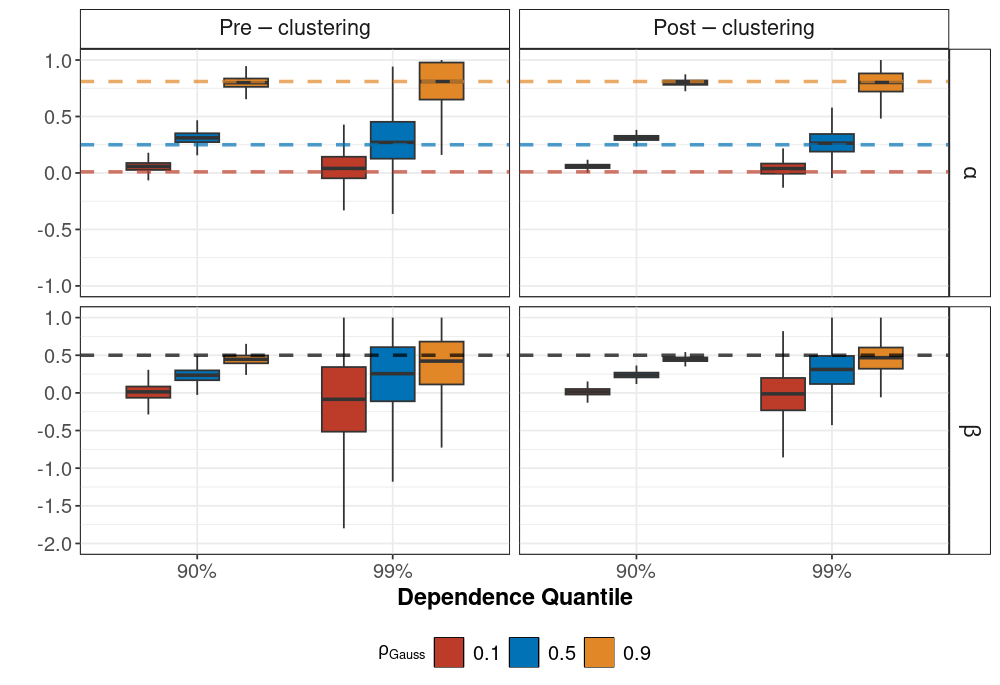
\includegraphics[width = 0.8\linewidth]{figure_1.png}
    \caption{\emph{ 
    Boxplots of estimates of $\alpha_{\mid i}$ (top) and $\beta_{\mid i}$ (bottom) for the conditional extremes model pre- and post-clustering with bivariate Gaussian data simulated at 12 sites, belonging equally to three known clusters. 
    The x-axis gives $q$, the level of the conditioning quantile used to fit the model, and the boxes are coloured by the true Gaussian copula correlation parameter, $\rho_{\text{Gauss}}^s$.
    The horizontal lines indicate the true theoretical values of $\alpha_{\mid i}$ and $\beta_{\mid i}$, with the colours for $\alpha_{\mid i}$ corresponding with the true $\rho_{\text{Gauss}}^s$ values.
    }}
   \label{fig:00_gauss_cop}
\end{figure}


\subsection{Mixture model setting}
\label{subsec:sim_mixture}

We extend our simulation design to mixtures of Gaussian and Student $t$-copulas \citep{Demarta2007-ap}, which induce asymptotic independence and asymptotic dependence, respectively, and whose dependence strength is determined by their respective correlation parameters $\rho_{\text{Gauss}}^s$ and $\rho_{\text{t}}^s \in [0, 1]$.

To obtain a sample of size $n = 1000$ from the mixture copula, at each site $s =1, \ldots, 12$, we combine $n/2 = 500$ samples from the Gaussian copula described in Section~\ref{subsec:sim_gauss} (with correlation parameter $\rhou{Gauss}^s$), and $n/2 = 500$ observations from a Student $t$-copula with 3 degrees of freedom and correlation $\rhou{t}^s$, before applying the Laplace transformation in Equation~\eqref{eq:laplace} to obtain the pairs $(Y_{1,s}, Y_{2,s})$ at site $s$.

In Section~\ref{subsubsec:sim_competing_methods}, we compare our method to the leading extremal competitor in the bivariate case \citep{Vignotto2021} and, in Section~\ref{subsubsec:sim_extension}, we show how our approach uniquely handles clustering of multivariate extremes in higher dimensions ($d > 2$).
Finally, Section~\ref{subsubsec:sim_realistic} considers a setting with $D = 60$ locations across three unequally sized clusters, and locations in the same cluster exhibiting perturbations in their correlation parameters.
Performance is evaluated using the ARI, with 500 replicated experiments per setting.

\subsubsection{Comparison to \citet{Vignotto2021}}
\label{subsubsec:sim_competing_methods}

When $d = 2$, we compare our extremal clustering method to that of \citet{Vignotto2021}.
We generate $n = 1000$ observations at $D = 12$ sites, using the mixture of Gaussian and t-copulas (with Laplace margins), as described above. 
Two clusters of sites $s = {1, \ldots, 6}$ and $s = {7, \ldots, 12}$ are defined with different values of $\rhou{t}^s$. 
We set $\rhou{t}^s = \rho_{\text{t}_1}$ for $s = 1, \ldots, 6$ and $\rhou{t}^s = \rho_{\text{t}_2}$ for $s = 7, \ldots, 12$, while $\rhou{Gauss}^s$ is the same for both clusters. 
We consider a range of extremal dependence scenarios defined over a grid of values $\left(\rhou{Gauss}^s \in \{0.1, 0.2, \ldots, 1.0\}, \rho_{\text{t}_1}^s \in \{0.1, 0.3, \ldots, 0.9\}, \rho_{\text{t}_2}^s \in \{0, 0.2, \ldots, 0.8\}\right)$.
We estimate the CE model using $q = 0.9$, and clusters were obtained using the aggregated dissimilarity matrix $M$ in Equation~\eqref{eq:aggregate_matrix}.

The results are shown in Figure~\ref{fig:01_ce_vs_vi}. 
Across the range of considered bivariate extremal dependence structures, our method consistently outperforms that of \citet{Vignotto2021}. 
Both methods have high ARI when the cluster-wise difference in $\rhou{t}^s$ is larger, since greater disparity naturally makes clusters more distinct and clustering easier. 
Both methods perform better when the Gaussian and t-copula correlations are higher.
This may be because the Gaussian copula becomes more similar to the t-copula for higher values of $\rhou{Gauss}$, thus allowing the clustering approach to focus on differences in the t-copula.

\begin{figure}[htb]
    \centering
    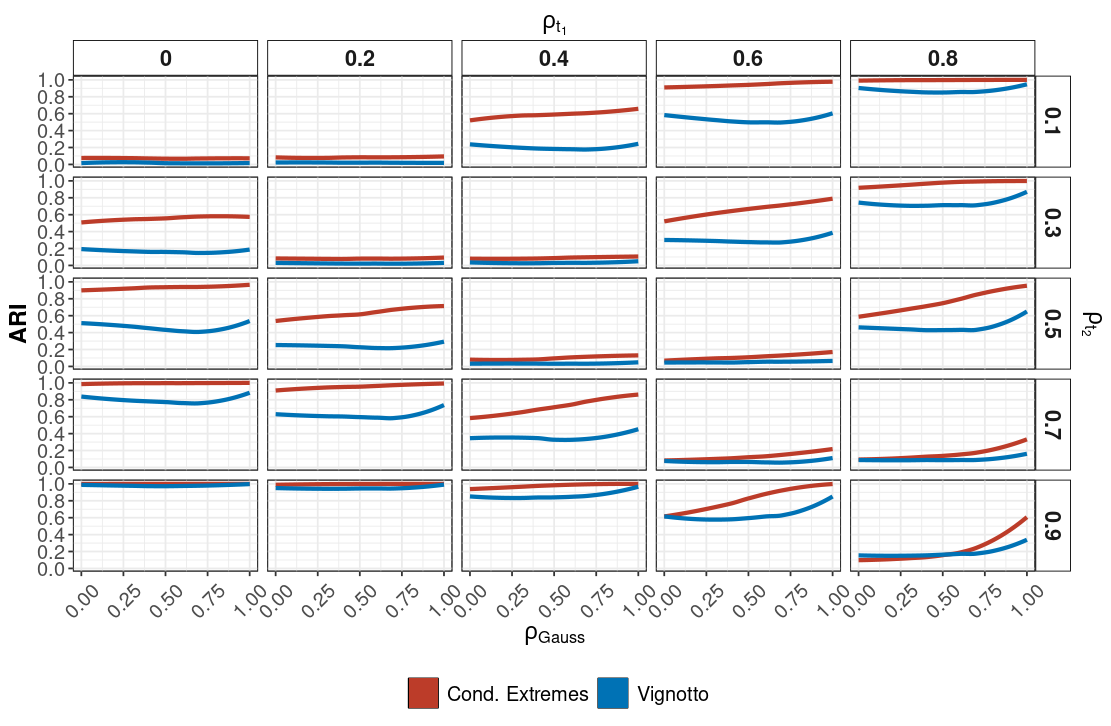
\includegraphics[width = 0.8\linewidth]{figure_2.png}
    \caption{\emph{
    Comparison of our conditional extremes-based approach and the method of \citet{Vignotto2021}.
    The x-axis represents the Gaussian correlation parameter $\rhou{Gauss}$, with facet labels indicating the t-copula correlation parameters, $\rho_{\text{t}_1}$ and $\rho_{\text{t}_2}$, for the two true clusters.
    The smoothed lines show the average ARI across bootstrap samples, for both methods, with smoothing performed using a generalised additive model.
    }}
    \label{fig:01_ce_vs_vi}
\end{figure}

\subsubsection{Extension to higher dimensions}
\label{subsubsec:sim_extension}

While the method of \citet{Vignotto2021} is restricted to $d = 2$ dimensions, our approach can be extended to $d \geq 3$ variables. 
To illustrate this, we extend the simulation study of Section~\ref{subsubsec:sim_competing_methods} by simulating at $D = 12$ locations, with two equally-sized clusters of sites each with $n = 1000$ observations per site, but now for $d = 3$ variables, using the same grid of ($\rhou{Gauss}, \rho_{\text{t}_1}, \rho_{\text{t}_2}$) values as in Section~\ref{subsubsec:sim_competing_methods}.
Our mixture copula now has three dimensions (with all pairwise correlations equal), and we fit three CE models at each site. 
Clustering is performed using the aggregated divergence matrix $M$ from Equation~\eqref{eq:aggregate_matrix}.
The results show that our proposed method performs well for $d =3$, with the same patterns in ARI emerging as in the bivariate case in Section~\ref{subsubsec:sim_competing_methods}.
In fact, performance is markedly stronger in three dimensions than in two. 
This is not surprising, as the CE fits in this setup are similar in both two and three dimensions, with the same $\rhou{t}^s$ being used across all variable pairs.
Therefore, the aggregated matrix $M$ in Equation~\eqref{eq:aggregate_matrix} is computed similarly, just averaged over more models with more data, which naturally improves clustering performance.

\begin{figure}[htb]
    \centering
    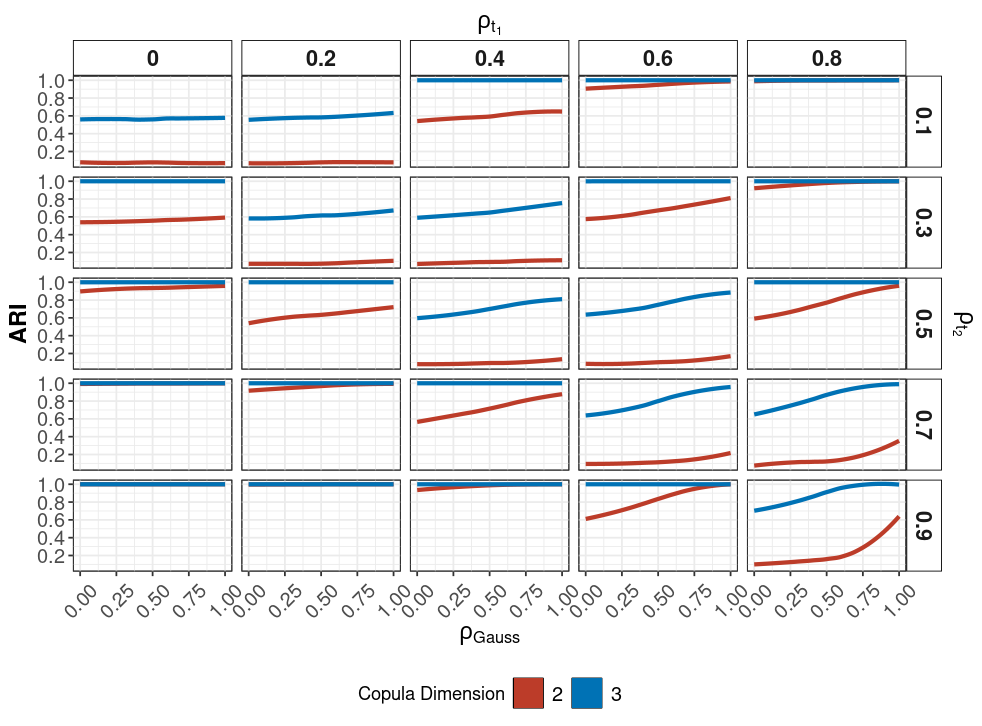
\includegraphics[width = 0.8\linewidth]{figure_3.png}
    \caption{\emph{
        Comparison of clustering performance for $d = 2$ and $d=3$ variables and two equally-sized clusters. 
        The x-axis represents the Gaussian correlation parameter $\rhou{Gauss}$ for both clusters, and the facet labels show the t-copula correlation parameters, $\rho_{\text{t}_1}$ and $\rho_{\text{t}_2}$, for the two true clusters.
        The smoothed lines show the average ARI across bootstrap samples, with smoothing performed using a generalised additive model.
    }}
   \label{fig:02_3d}
\end{figure}


% Expand to up to 5 dimensions!
To further illustrate the performance of our method in higher dimensions, we consider a specific case from the grid where $\rho_{\text{t}_1} = 0.4$ and $\rho_{\text{t}_2} = 0.5$. 
This setting presents a challenging clustering scenario in both two and three dimensions, as the cluster-wise difference in the t-copula correlation parameters is small. 
Figure~\ref{fig:02b_5d} displays the results when the dimensionality of the copula mixture is increased from $d = 2$ to $d = 5$, based on 500 simulations across all considered $\rhou{Gauss}$ values. 
Cluster accuracy improves steadily with dimension, reaching values close to 1 across all $\rhou{Gauss}$ settings when $d = 5$. 
These gains should be interpreted cautiously, since as mentioned above we use the same $\rhou{t}^s$ across all variable pairs, thus not altering the pairwise extremal dependence structure and instead increasing the amount of data as $d$ increases.
Having separate $\rhou{t}^s$ values for each variable pair would increase the complexity and signal-to-noise ratio of the clustering task, and likely reduce performance.
Nevertheless, the results demonstrate that the proposed method scales effectively to higher dimensions and performs well in multivariate settings. 

\begin{figure}[htb]
    \centering
    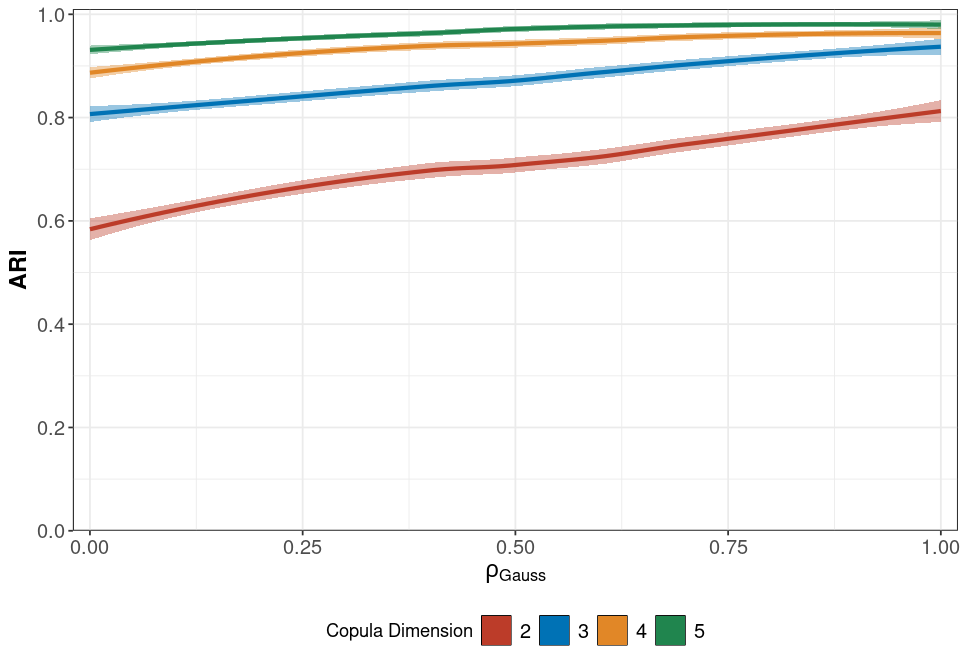
\includegraphics[width = 0.7\linewidth]{figure_4.png}
    \caption{\emph{
        Evaluation of clustering for $d = 2$ to $d = 5$ variables and two equally-sized clusters for simulations at 12 sites from a mixture of Gaussian and t-copulas.
    The t-copula correlation parameters for each true cluster were set to $\rho_{\text{t}_1} = 0.4$ and $\rho_{\text{t}_2} = 0.5$. 
A sequence of values are considered for the Gaussian correlation parameter $\rhou{Gauss}$, as represented on the x-axis.
    The smoothed lines show the average ARI and associated uncertainty across bootstrap samples, with smoothing performed using a generalised additive model.
}}
\label{fig:02b_5d}
\end{figure}

\subsubsection{Extension to more sites}
\label{subsubsec:sim_realistic}

We now design another simulation study to better mimic the structure of the Irish meteorological dataset, to be analysed in Section~\ref{sec:application}. 
Data are generated at $D = 60$ sites, each with $n = 1000$ observations of $d = 2$ variables, using the mixture of Gaussian and t-copulas.
The 60 sites are partitioned into three unequally-sized clusters of 10, 20, and 30 sites. 
At each location, the true $\rho_{\text{t}}^s$ is perturbed by adding $\text{Unif}(-0.05, 0.05)$ noise, making the clustering task more challenging.
We now have a separate t-copula correlation parameter for each of the three clusters, denoted by $\rho_{\text{t}_1}, \rho_{\text{t}_2}$, and $\rho_{\text{t}_3}$.
To reduce the dimensionality of the grid of considered copula parameter values, a constant $\rhou{Gauss} = 0.5$ is used across all sites and experiments. 

% results
The results of 500 repetitions of this simulation study are shown in Figure~\ref{fig:03_realistic}.
Similarly to the previous simulation studies, our clustering method performs well, particularly when the differences in t-copula correlation parameters between clusters are larger. 
For example, the best performance is observed where $\rho_{\text{t}_1} = 0.9, \rho_{\text{t}_2} = 0.1$, and $\rho_{\text{t}_3} = 0.5$, as the clusters are most distinct, while conversely, performance is worst for $\rho_{\text{t}_1} = 0.6, \rho_{\text{t}_2} = 0.4$, and $\rho_{\text{t}_3} = 0.5$. % \todo{Include this to aid reading of figure, is it necessary?}

\begin{figure}[htb]
    \centering
    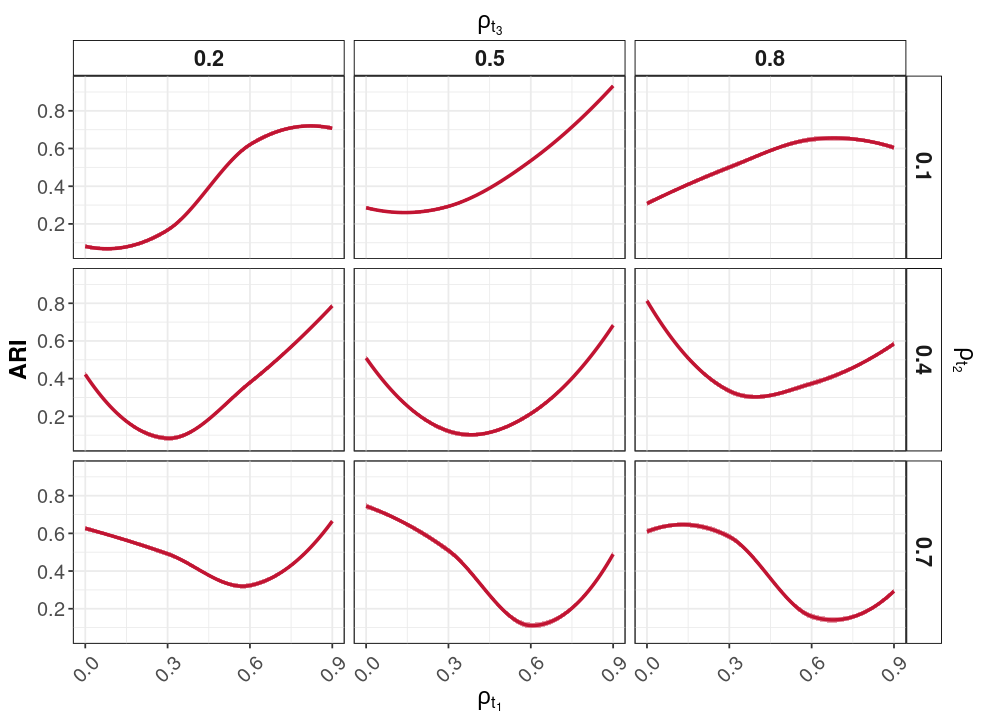
\includegraphics[width = 0.7\linewidth]{figure_5.png}
    \caption{\emph{Evaluation of clustering performance for $d = 2$ variables and three clusters of 60 locations for simulations from a mixture of Gaussian and t-copulas.
        The true x-axis and facet labels show the t-copula correlation parameters,  $\rho_{\text{t}_1}, \rho_{\text{t}_2}$, and $\rho_{\text{t}_3}$, for each of the three true clusters, for a Gaussian copula correlation of $\rhou{Gauss} = 0.5$. 
    The smoothed lines show the average ARI across bootstrap samples, with smoothing performed using a generalised additive model. 
    }}
   \label{fig:03_realistic}
\end{figure}

\section{Application to Irish meteorological data}
\label{sec:application}
% Section Intro
We now apply our extremal clustering method to meteorological observations from the Republic of Ireland. 
In Section~\ref{subsec:app_data}, we describe the precipitation and wind speed measurements used in our analysis and present exploratory analysis (using the $\chi$ statistic from Equation~\eqref{eq:chi}) on the extremal dependence between the two variables. 
In Section~\ref{subsec:app_ce}, we discuss fits of the conditional extremes (CE) model, and, in Section~\ref{subsec:app_clust}, we apply our extremal clustering approach. 

\subsection{Ireland meteorological data}
\label{subsec:app_data}

\begin{figure}[htb]
    \centering
    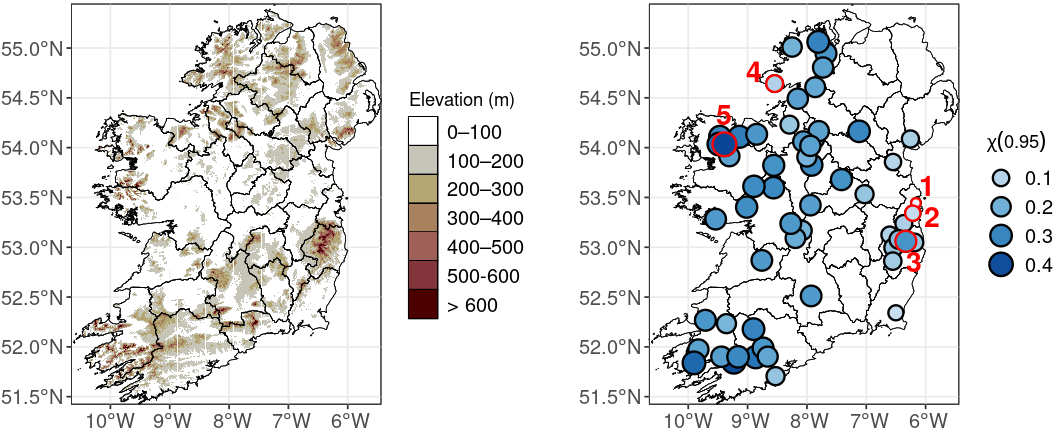
\includegraphics[width = 0.8\linewidth]{figure_6.png}
    \caption{\emph{
    Left: elevation (m) profile of Ireland.
    Right: Estimated $\chi(0.95)$ between precipitation and wind speed at all 59 locations. Darker colours and larger points indicate stronger asymptotic dependence.
    Locations in red are (1) Malahide Castle, Dublin, (2) Ringsend, Dublin, (3) Glenmacnass, Wicklow, (4) Kilcar, Donegal, and (5) Derryhillagh, Mayo.
}}
   \label{fig:chi}
\end{figure}

We analyse the joint extremal behaviour of precipitation and wind speed at $D=59$ sites across the Republic of Ireland from 1990 to 2020, inclusive. 
Precipitation and wind speed data are obtained from the Met Éireann archive \citep{metHistoricalData}, and ERA5 Reanalysis \citep{Hersbach2020}, respectively. 
Met Éireann data are irregularly spaced over space, while ERA5 provides spatial averages on a regular $0.25^{\circ} \times 0.25^{\circ}$ grid.
We match each spatial site to the grid cell in which it lies. 
The dataset spans 11,323 consecutive daily observations.

% Preprocessing
We focus on the winter months, October to March, following \citet{Vignotto2021}.
Precipitation are aggregated into weekly sums, and daily wind speed maxima are aggregated into weekly averages.
This weekly temporal scale reflects the typical lag between extreme precipitation and wind speed during storm events \citep{Bengtsson2009}, and reduces short-term temporal dependence not accounted for in our model. 
Weeks with no precipitation are excluded, resulting in 5,022 observations across all $D = 59$ sites. 

% Chi statistic
We explore the extremal dependence structure of the data using the $\chi$ statistic introduced in Equation~\eqref{eq:chi}.
Figure~\ref{fig:chi} shows empirical estimates of $\chi(0.95)$ at all 59 sites.
An elevation profile of Ireland is also shown in Figure~\ref{fig:chi}, which may help further explain some of this spatial structure.
Non-zero values are observed at almost all sites, indicating positive extremal dependence between precipitation and wind speed. 
In practical terms, this suggests that extreme wind speeds tend to be accompanied by high precipitation, and vice versa. 
A clear spatial pattern emerges: extremal dependence is strongest in the south west, with the highest values along the Atlantic coast, notably in counties Kerry, Galway, Mayo, and Donegal, and weaker along the east coast, in Dublin, Wexford, and Louth. 
The highest $\chi(0.95)$ value (0.414) is observed at Derryhillagh in Mayo (Figure~\ref{fig:chi}, location (5)), while the lowest (0.0005) is at Malahide Castle in Dublin (Figure~\ref{fig:chi}, location (1); hereafter `Malahide').

Some spatial outliers are also apparent. 
Kilcar in Donegal (Figure~\ref{fig:chi}, location (4)) has a relatively low $\chi(0.95)$ value (0.109), despite its west-coast location, while some sites in county Wicklow show unusually high values for the east, particularly Glenmacnass (Figure~\ref{fig:chi}, location (3); 0.268).
The latter may be related to the influence of the Wicklow Mountains, as reflected in the elevation profile (Figure~\ref{fig:chi}). 
It may be of interest to investigate if these outliers in $\chi(0.95)$ are reflected in the CE model parameter estimates, and whether clustering can identify them.
These results indicate distinct regional patterns of extremal dependence, as well as notable outliers, motivating the use of our extremal clustering framework to characterise and interpret this spatial structure more formally. 

\subsection{Conditional extremes estimates}
\label{subsec:app_ce}

% Procedure and results pre-clustering (choice of quantile)
We transform the precipitation and wind speed data, separately at each location, to Laplace margins, with the empirical rank transform replacing $F_{X_i}$ in Equation~\eqref{eq:laplace}.
To select an appropriate quantile level $q$ for fitting the CE model (see Section~\ref{subsec:ce_model}), we estimate the parameters $(\alpha_{\mid i}, \beta_{\mid i})$ at a sequence of levels $q$, to identify the lowest $q$ beyond which parameter estimates appear stable.
Estimates are generally stable for both models, i.e.,\@ precipitation conditional on wind speed and vice versa, down to $q = 0.85$, with similar maximum likelihood estimates across 500 bootstrap samples for $(\alpha_{\mid i}, \beta_{\mid i})$.
Threshold stability plots for the CE fits at the five locations highlighted in Figure~\ref{fig:chi} are included in Figures~\ref{fig:boot_quantiles_malahide} -- \ref{fig:boot_quantiles_derryhillagh} of the supplementary materials.
Therefore, we fix $q = 0.85$ for the subsequent analysis.
In Figure~\ref{fig:clust_sens}, we show that our estimated extremal clustering is robust to the choice of $q$, with estimates shown for $q = 0.85, 0.88$, and $0.90$.

The estimated site-wise CE parameters are shown in Figure~\ref{fig:a_b_vals}.
Although interpretation is challenging due to variability in the estimates, as with the $\chi(0.95)$ estimates (Figure~\ref{fig:chi}), we observe some evidence of increasing $\alpha_{\mid i}$ values for both variables towards the west and south.
To mitigate uncertainty and aid interpretation, we cluster the locations using our extremal clustering approach. 

\begin{figure}[htb]
    \centering
    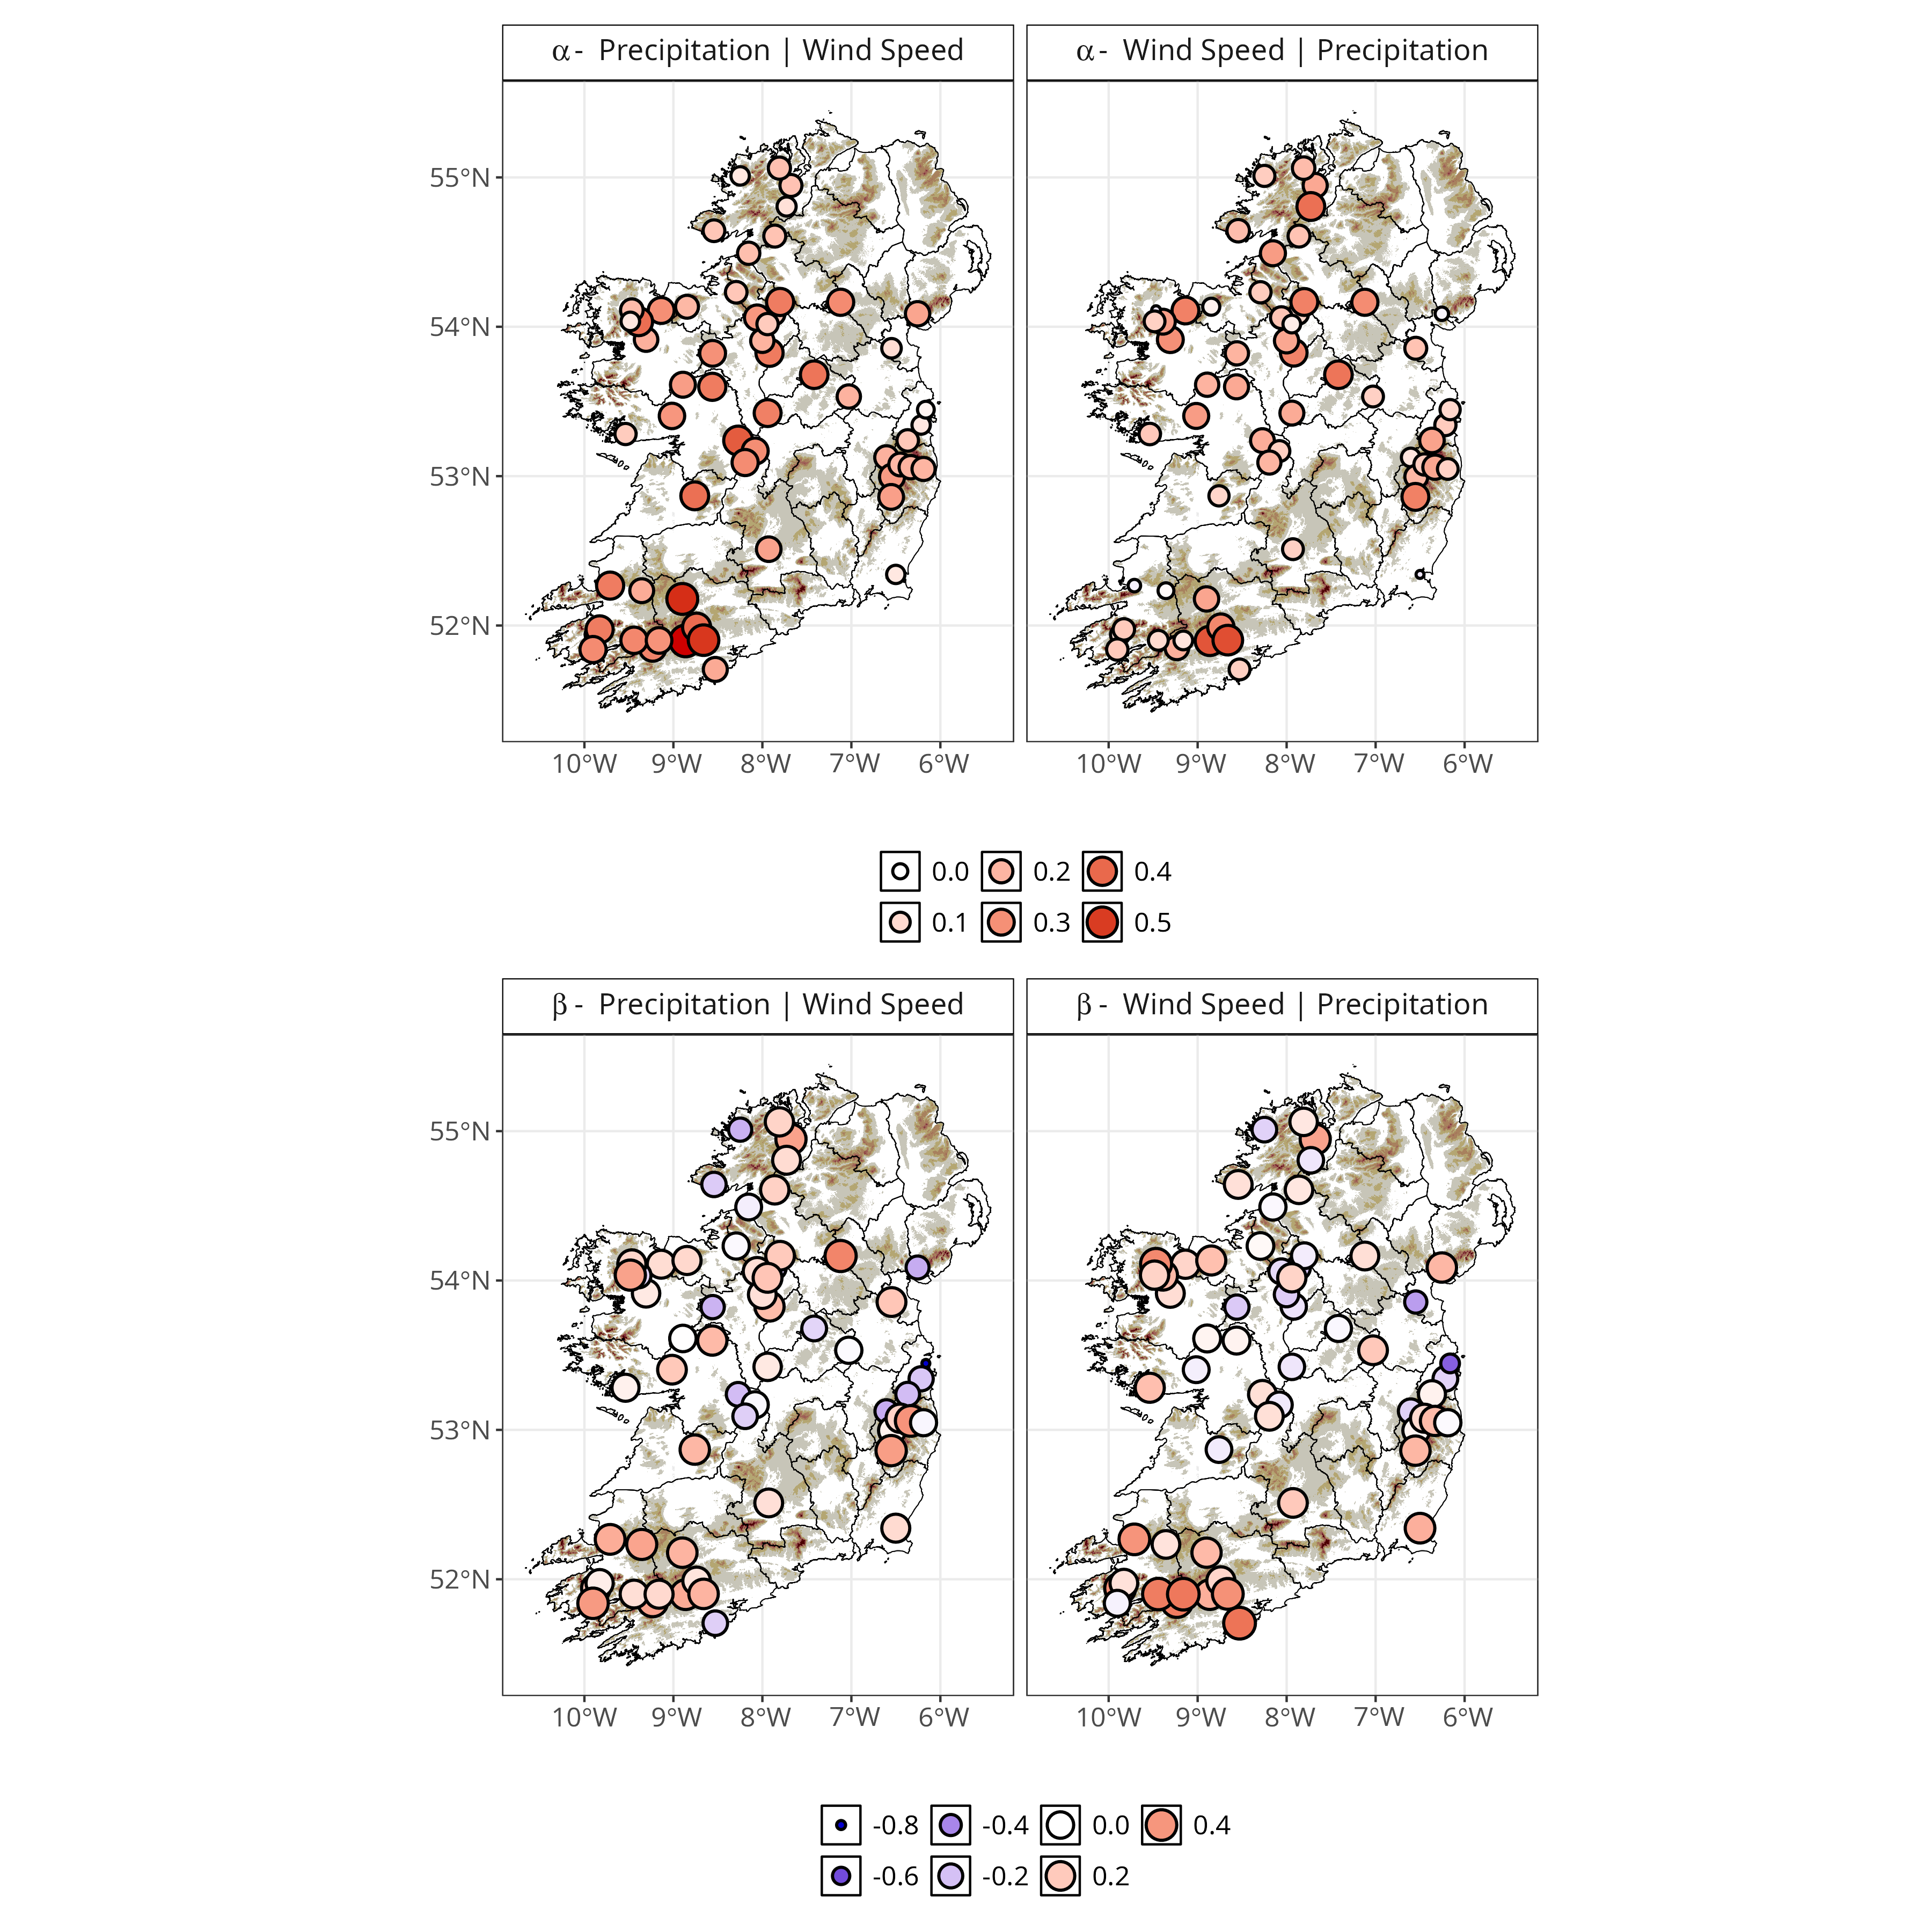
\includegraphics[width = 0.8\linewidth]{figure_7.png}
    \caption{\emph{
        Maps of site-wise estimated model parameters $\alpha_{\mid i, s}$ (top) and $\beta_{\mid i, s}$ (bottom) for precipitation conditional on wind speed (left) and wind speed conditional on precipitation (right).
        The colour scale is the same for both variables, with darker red and larger points indicating larger positive values of $\alpha$ and $\beta$, and darker blue and smaller points indicating smaller negative values.
   }}
   \label{fig:a_b_vals}
\end{figure}


\subsection{Clustering}
\label{subsec:app_clust}

We cluster the locations using the aggregated dissimilarity matrix $M$ as defined in Equation~\eqref{eq:aggregate_matrix}, and separately for each individual matrix $M^{(i)}, i = 1, 2$, as in Equation~\eqref{eq:distance_matrix}.
The number of clusters $k$ is chosen via the method in Section~\ref{subsec:clustering}, using the elbow plot of the $\mathrm{TWGSS}$. 
For all three clustering scenarios, clear elbows are observed at $k = 3$.
The elbow plots are provided in Figure~\ref{fig:elbow_plots} of the supplementary materials. 

The resulting cluster estimates are displayed in Figure~\ref{fig:clust_sol}.  
Across all three choices of dissimilarity matrix, the estimated clusters are broadly consistent, with three spatially distinct groups emerging.  
This spatial coherence is notable given that no explicit spatial information was used in model fitting or in the clustering, suggesting that the CE model parameters capture meaningful spatial structure in the extremal dependence of the data. 

When interpreting the clusters, we observe a clear contrast between the east and west coasts, separated by a central cluster.  
For precipitation conditional on wind speed, the clustering is somewhat less distinct, with the central cluster extending more extensively into parts of Galway, Mayo, and Donegal on the west coast.  
There are also notable outliers in the clusters, which we further discuss below. 

\begin{figure}[htb]
    \centering
    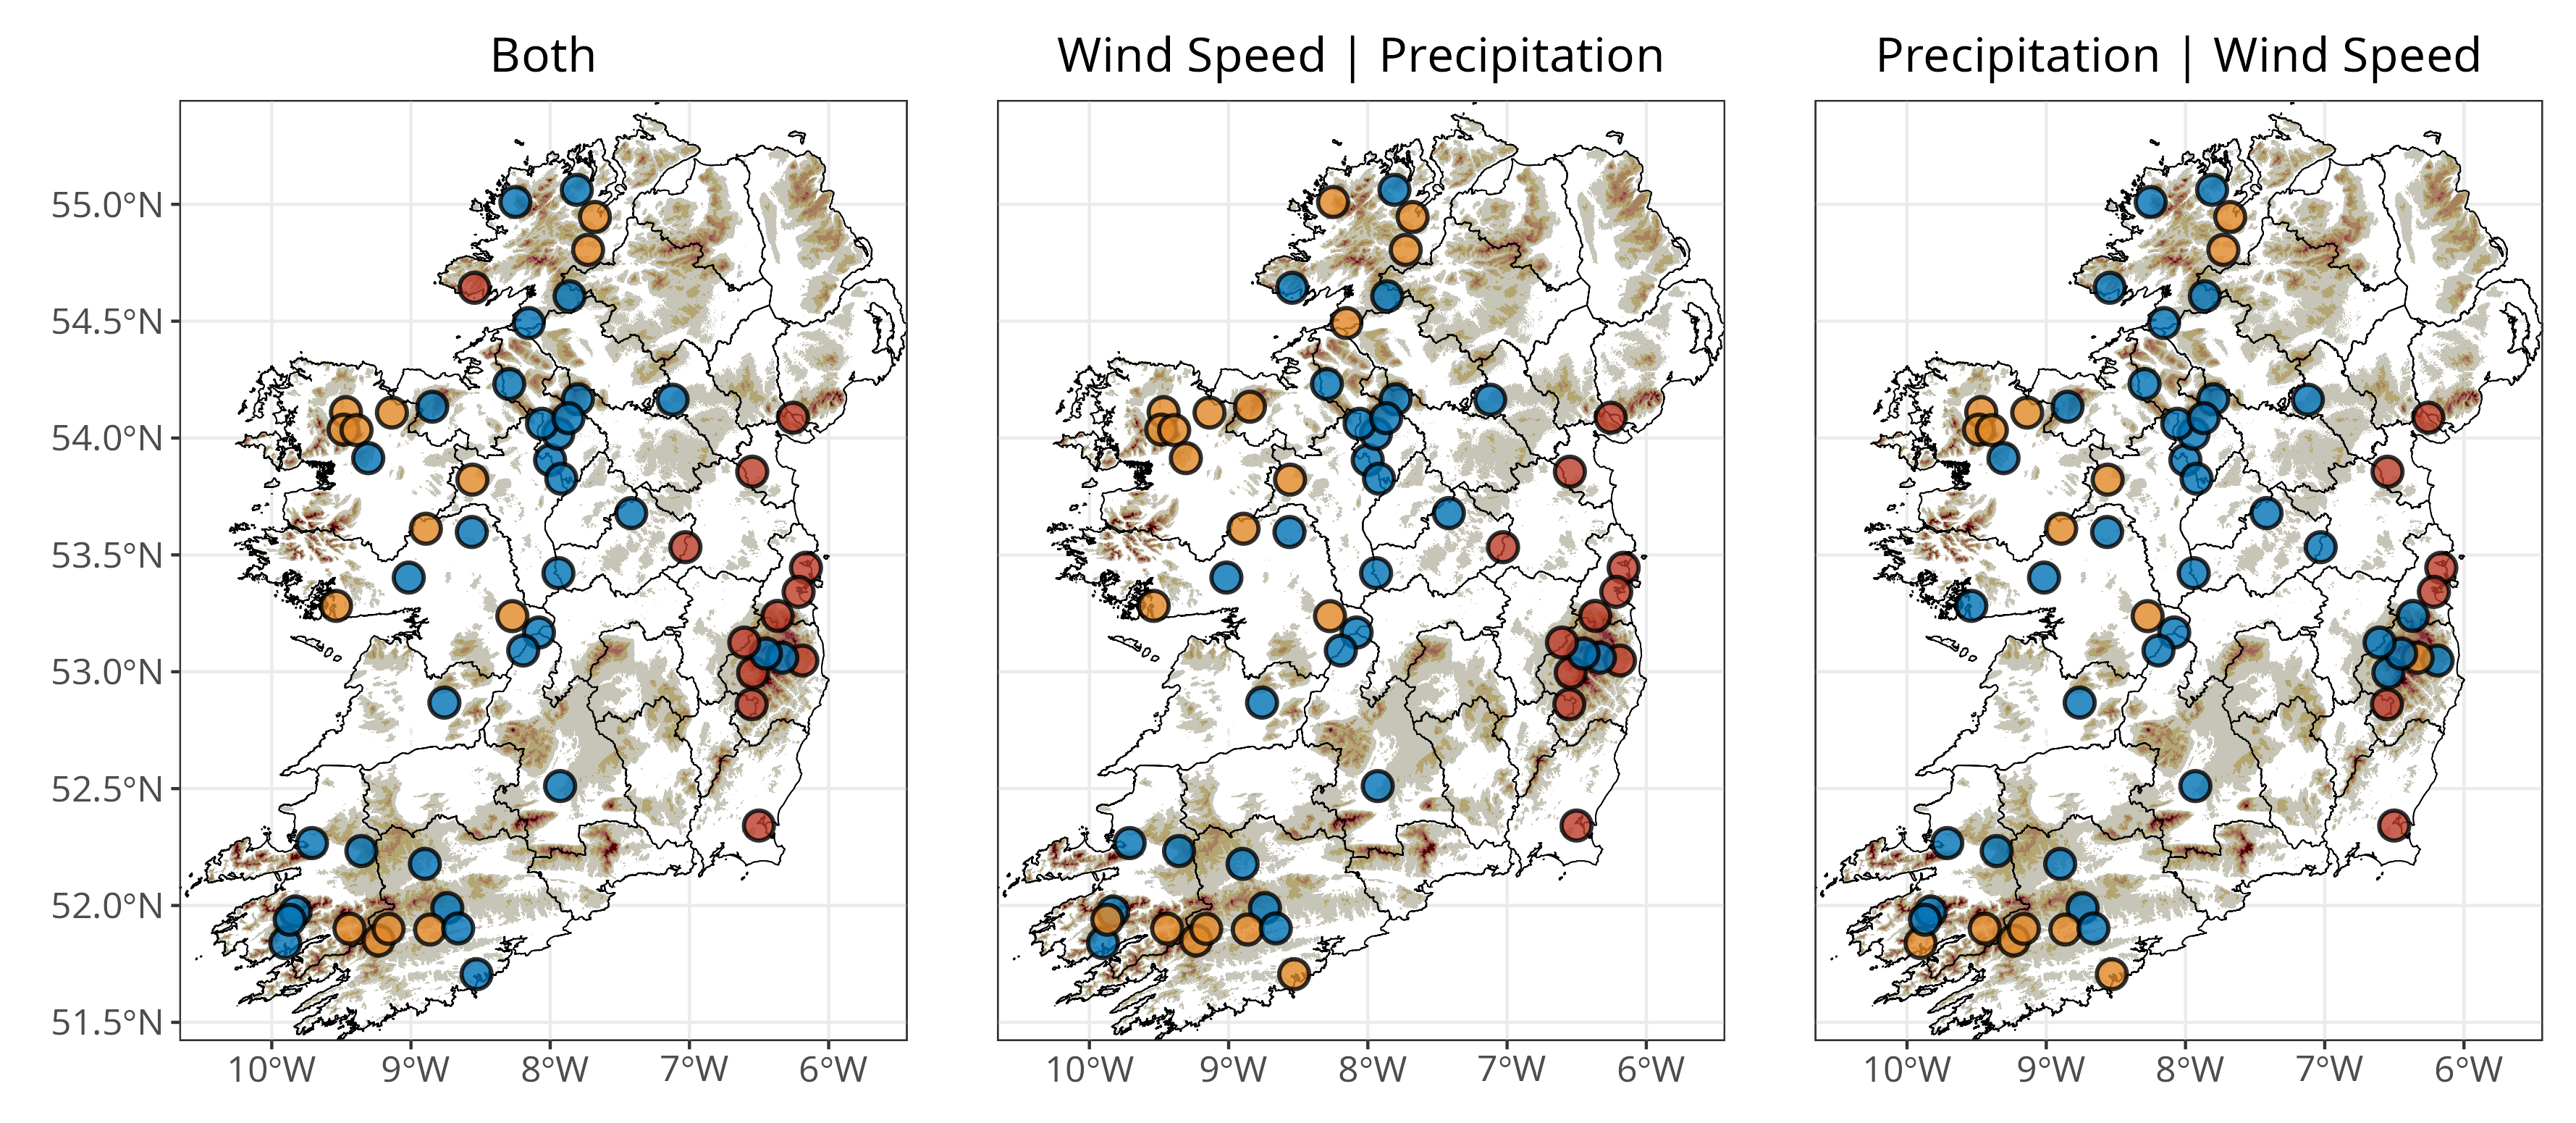
\includegraphics[width = 0.8\linewidth]{figure_8.png}
    \caption{\emph{
    Extremal cluster estimates using the dissimilarity matrix for wind speed conditional on precipitation (centre), precipitation conditional on wind speed (right), and the combined dissimilarity matrix (left). 
    Sites are coloured by cluster label.
}}
\label{fig:clust_sol}
\end{figure}

\begin{figure}[htb]
    \centering
    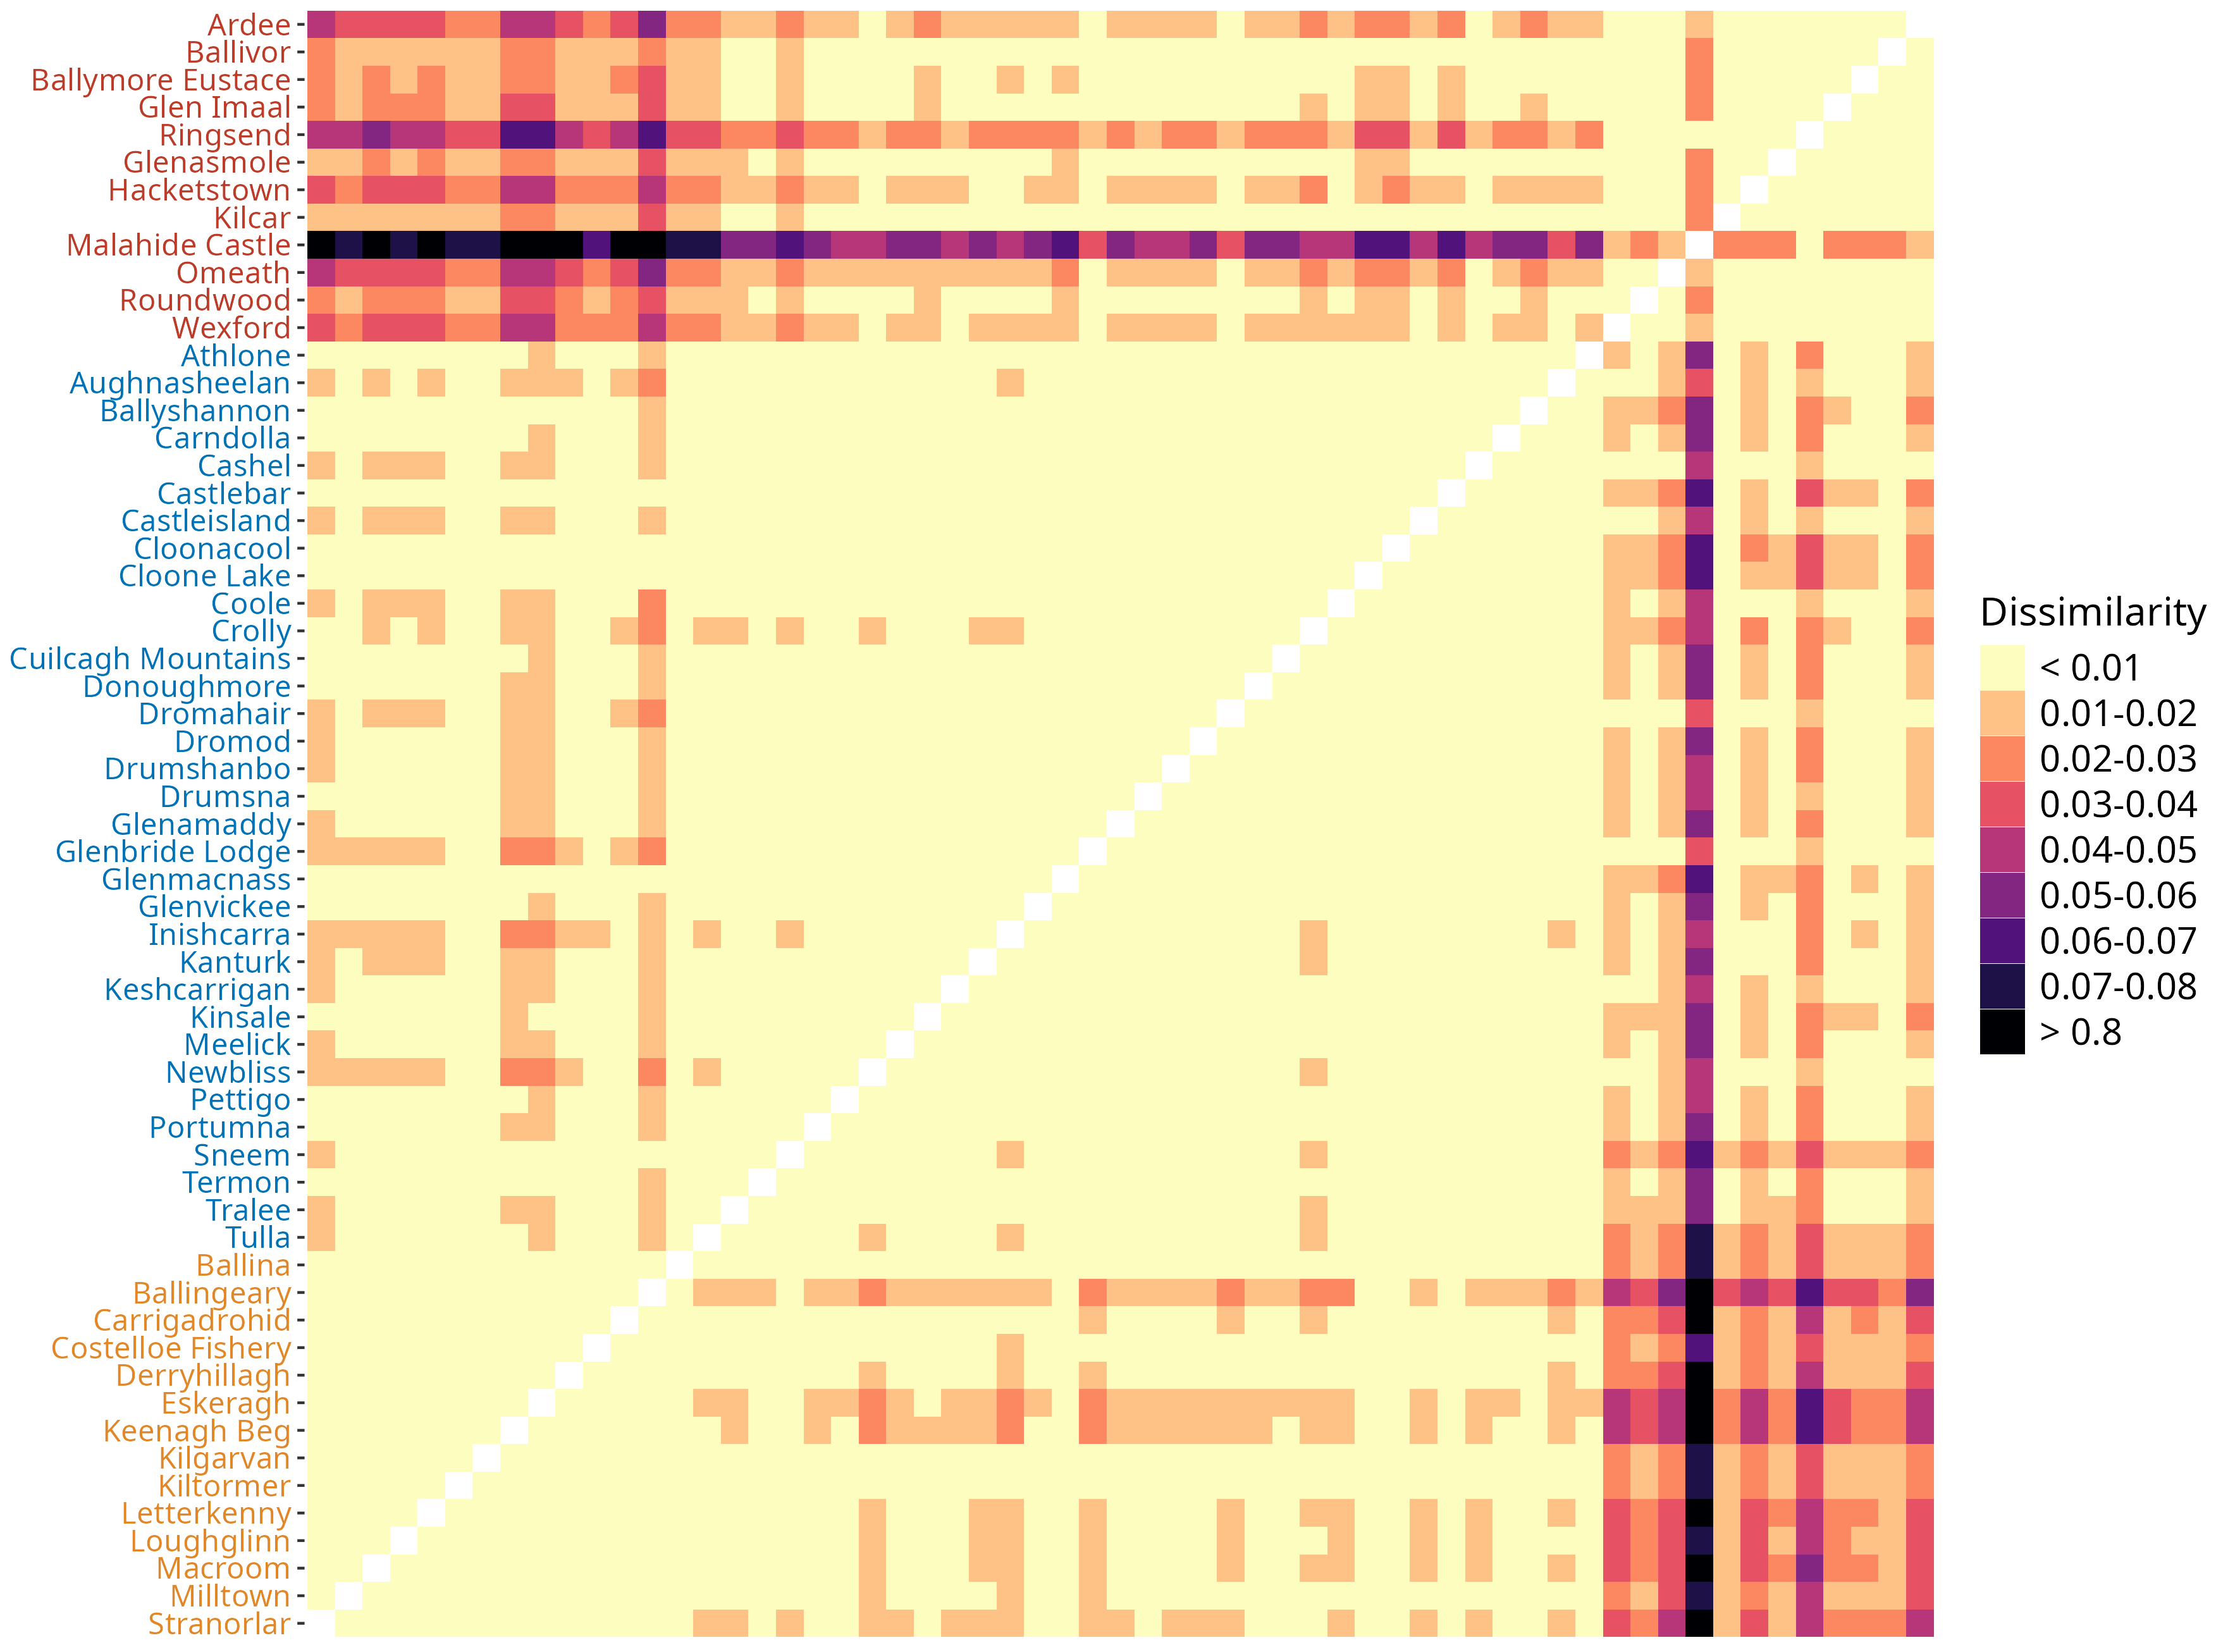
\includegraphics[width = 1.0\linewidth]{figure_9.png}
    \caption{\emph{
    Heatmap of the estimated aggregated dissimilarity matrix $M$.
The names of each site are coloured and ordered according to their estimated cluster labels, matching that of Figure \ref{fig:clust_sol}. 
The dissimilarity colour scale is shown on the right, with darker colours indicating larger values.
}}
\label{fig:dist_heatmap}
\end{figure}

% Analysis of dissimilarity matrix
In Figure~\ref{fig:dist_heatmap}, we visualise the dissimilarity matrix for the aggregated clusters (see left panel of Figure~\ref{fig:clust_sol}).
The clusters are quite distinct, with the dissimilarity between clusters being much larger than within-cluster dissimilarity, which rarely exceeds 0.01.
In particular, the difference between the eastern and western clusters is quite pronounced, with the intermediate central cluster acting as somewhat of a `buffer' between the two.
In contrast, the western and central clusters seem to be quite close, in that we observe many small inter-cluster pairwise dissimilarities between them. 
This indicates that allocation between the two is not always clear-cut and for several sites is nearly interchangeable, as observed in  the variable-specific estimated clusters in Figure~\ref{fig:clust_sol} and in the quantile sensitivity analysis in Figure~\ref{fig:clust_sens}, where membership between the two often switches. 
Also, if we only fit two clusters, we find that most of the central cluster members are assigned to the western cluster, reflecting this less obvious separation between the two compared to the more markedly different eastern cluster. 
A noticeable outlier in the dissimilarity matrix is Malahide, which we previously identified as having the lowest $\chi(0.95)$ value  in Figure~\ref{fig:chi}. 
Even within its own cluster, Malahide shows a relatively high dissimilarity to the other sites. 
Indeed, if we set $k=4$, Malahide becomes its own cluster (clustering results for $k=2$ and $k=4$ are provided in Figure~\ref{fig:cluster_dqu_k_2_4} of the supplementary materials).
Malahide also has the lowest mean weekly precipitation of any site; the second lowest is Ringsend, also in county Dublin (Figure~\ref{fig:chi} location (2)), which is the site closest to Malahide in terms of our dissimilarity measure. 
Finally, Malahide has very low $\chi(0.95)$ (Figure~\ref{fig:chi}) and $\alpha_{\mid i}$ (Figure~\ref{fig:a_b_vals}) estimates. 
Together, this may explain why we observe such outlying behaviour for Malahide.
Finally, Kilcar in County Donegal is the member of the eastern cluster with the smallest dissimilarity to the western cluster members.
This may reflect its geographic location in northwest Ireland, despite it's low $\chi(0.95)$ value (Figure~\ref{fig:chi}) relative to other west-coast sites.

\begin{figure}[htb]
    \centering
    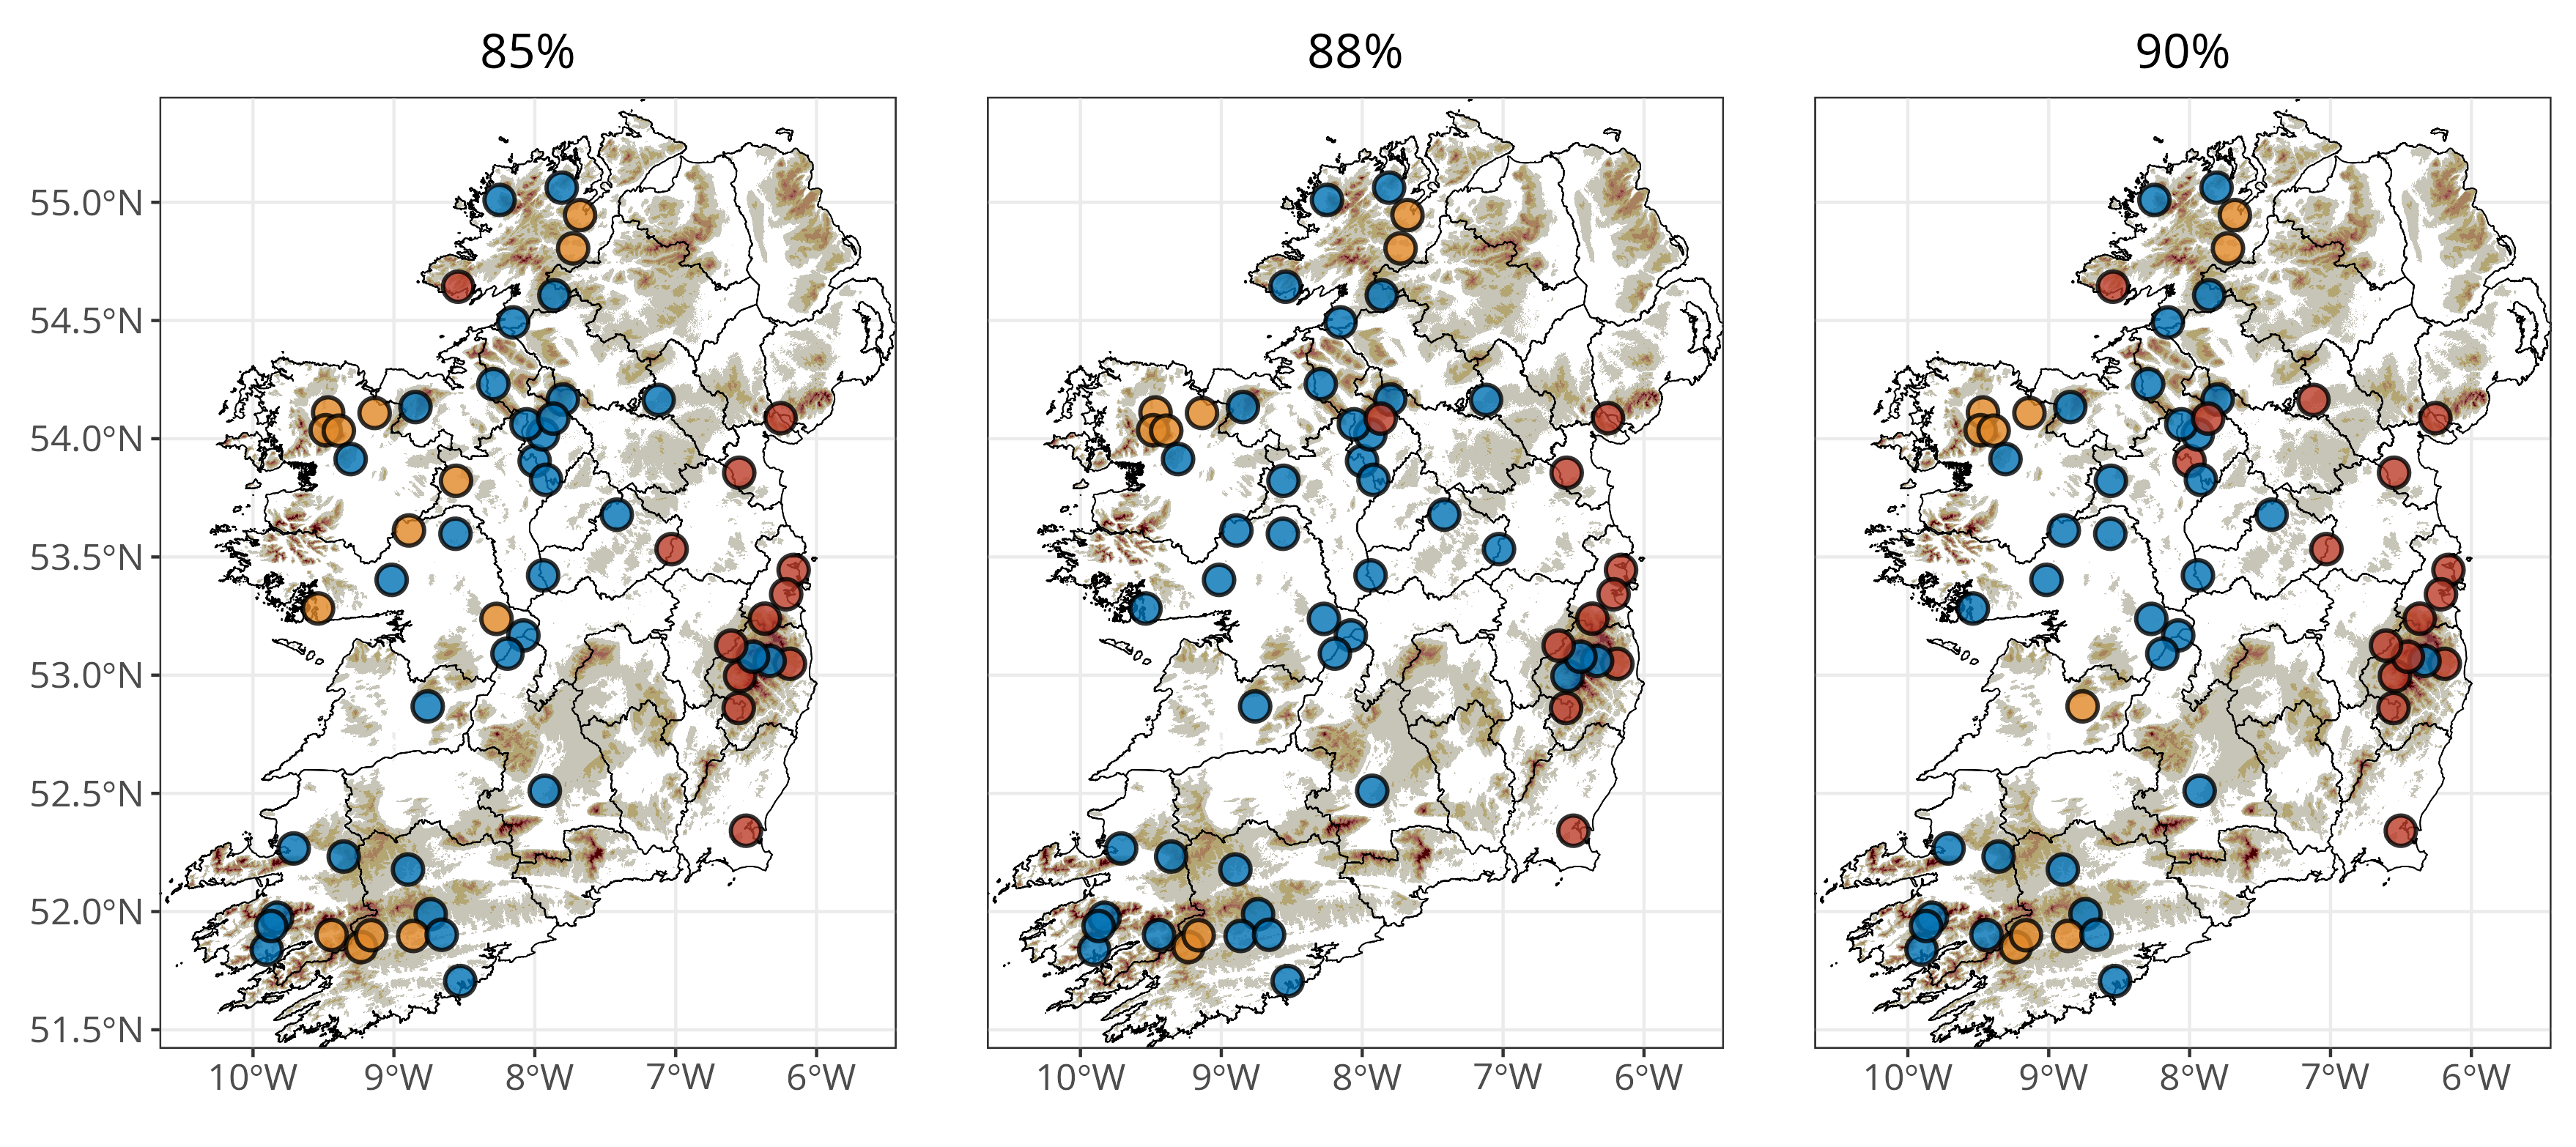
\includegraphics[width = 0.85\linewidth]{figure_10.png}
    \caption{\emph{
    Estimated extremal clusters with the conditional extremes model parameters estimated at $q = 0.85, q = 0.88$ and $q = 0.9$ quantiles, using the aggregated dissimilarity matrix. 
    Sites are coloured by cluster label. 
}}
\label{fig:clust_sens}
\end{figure}


% Sensitivity Analysis (to choice of DQU)
We perform a sensitivity analysis of the estimated clusters (with the aggregated dissimilarity matrix) to the choice of quantile level $q \in \{0.85, 0.88, 0.90\}$, in Figure~\ref{fig:clust_sens}.
The estimated clusters are similar across the three values of $q$, with some small differences. 
Noticeably, the earlier identified outlier at Kilcar in county Donegal is assigned to the eastern cluster when $q = 0.85$ and $q = 0.90$, but to the central cluster when $q = 0.88$.
Also, there are more sites in the western cluster when $q = 0.85$, with some sites moving to the central cluster for $q = 0.88$.
Interestingly, some of these sites then move back to the western cluster for $q = 0.90$.
Apart from these observations, the estimated clusters are generally quite similar across the three quantile levels, and so we conclude that our clustering method is relatively robust to the choice of quantile level.

\section{Discussion}
\label{sec:discuss}

% Quick summary
In this paper, we introduced a novel method for clustering multivariate extremes.
We proposed the expected conditional $\JSGa{}$ divergence \citep{Nielsen2019} as a measure of dissimilarity between multivariate conditional extremes (CE) models \citep{Heffernan2004}.
We leveraged the commonly-applied working Gaussian assumption to derive a closed-form expression for the $\JSGa{}$ divergence.
Efficient k-medoids clustering was then performed on the dissimilarity matrix derived from this measure. 
In our simulation study, a bivariate Gaussian copula example illustrated that our clustering method reduces parameter uncertainty and bias when the CE model is re-fitted with data pooled post-clustering.
Using mixtures of Gaussian and $t$-copulas, we showed that our method outperforms the method of \citet{Vignotto2021} across a range of bivariate extremal dependence scenarios.
Our method was also shown to be uniquely extendable to $d > 2$ dimensions. 
We applied our extremal clustering method to Irish meteorological data, consisting of 59 locations with weekly rainfall and wind speed observations.
Without explicitly incorporating spatial information, three clusters with distinct spatial patterns were identified, with well separated clusters representing the east and west coasts and the centre of Ireland.

% Extension
While we focused on a spatial application in this work, our method is more generally applicable to any setting where clustering of multivariate extremal dependence is desired.
For instance, it could be applied to clinical trial or public health data to cluster patients based on the tail dependence structure of their symptoms or biomarker measurements.
A neuroscience application was explored in \citet{Talento2025}, where the CE framework was used to highlight differences in the tail dependence of electroencephalogram (EEG) signals for seizure-prone and seizure-absent subjects. 
However, they used pre-defined clusters. Hence, we may expect our approach to be useful in similar applications, to identify subjects who have undergone extreme brain events, e.g., seizures.
In financial applications, we could cluster time periods according to the extremal dependence of log-returns of different assets, offering potential insights for portfolio management and risk assessment.

% Limitations: Gaussian assumption
While the residual Gaussian assumption on which our method relies may not hold for all datasets, our clustering approach showed good performance for all settings in Section~\ref{sec:sim}.
A possible alternative is to employ the generalised and asymmetric multivariate Gaussian distribution used in \citet{Farrell2025}. 
While this does not permit a closed-form divergence, our extremal clustering method could still be used, with costly numerical techniques used to estimate the dissimilarity matrix.
Indeed, if choosing to forgo this Gaussian assumption, it may be preferable to use the standard Jensen-Shannon divergence in place of the $\JSGa{}$ divergence, since the former is bounded \citep{Thiagarajan2025}.

% Limitations: Uncertainty
Another important limitation of our method is in its treatment of uncertainty.
We do not propagate uncertainty in the CE model estimates through to the clustering. 
To account for this, one possible approach is to use the bootstrap method of \citet{Heffernan2004} to generate samples of CE model estimates, and compute our dissimilarity matrix for each sample. 
We could then produce a distribution of dissimilarity matrices, and use these to compute a distribution of estimated clusters.
However, this would be computationally expensive, and so would compromise one of the main advantages of our method, namely its computational efficiency.

% Future work
In this work, we implicitly assume spatial stationarity in the extremal dependence structure, as we fit a separate CE model at each location.
Extensions of the CE model have been proposed, such as those incorporating covariates \citep{Richards2023} and spatio- and spatio-temporal representations of the CE parameters \citep{Simpson2021, Wadsworth2022}.
These could be incorporated into our clustering framework, but care must be taken to ensure that the residual Gaussian assumption still holds, or that an appropriate alternative dissimilarity is used, as discussed above.
Another approach to dealing with the uncertainty in the clustering solution would be to adopt a Bayesian perspective.
By placing priors on the CE model parameters, we could obtain posterior distributions for these parameters, which could be used to compute a distribution of dissimilarity matrices and clustering solutions.
Approaches such as that of \citet{Rohrbeck2021} have used a Reversible-Jump MCMC scheme to perform Bayesian clustering for spatial extremes, which does not require the number of clusters to be specified in advance.



% \section*{Acknowledgements}
% 
% \if0\blind
% {%
% Patrick O'Toole is supported by a scholarship from the EPSRC Centre for Doctoral Training in Statistical Applied Mathematics at Bath (SAMBa), under the project EP/S022945/1.
% We acknowledge the use of the ERA5 reanalysis dataset, available from the Copernicus Climate Change Service (C3S) Climate Data Store (CDS) (\url{https://cds.climate.copernicus.eu/}). 
% We also acknowledge the use of the Irish meteorological dataset obtained from Met Éireann (\url{https://www.met.ie/climate/available-data/historical-data}).
% } 
% \else
% {%
% We acknowledge the use of the ERA5 reanalysis dataset, available from the Copernicus Climate Change Service (C3S) Climate Data Store (CDS) (\url{https://cds.climate.copernicus.eu/}). 
% We also acknowledge the use of the Irish meteorological dataset obtained from Met Éireann (\url{https://www.met.ie/climate/available-data/historical-data}).
% }
% \fi


\begin{center}
{\large\bf SUPPLEMENTARY MATERIAL}
\end{center}

\begin{description}

  \item[PDF Supplement:] This supplement contains additional plots for the motivating data application in Section~\ref{subsec:app_clust} of the main paper, including elbow plots for choosing the number of clusters, clustering solutions for $k=2$ and $k=4$ clusters, and threshold stability plots for the conditional extremes model fits for the five locations highlighted in Figure~\ref{fig:chi}.

  \item[Data and R code:] The proposed methods are made available in an R package (link omitted for blind review).
    The analysis code used in the paper and the data are available upon request from the corresponding author.

\end{description}

% \typeout{=== TEX DIAGNOSTIC: before checking .bbl ===}
% \IfFileExists{manuscript_anonymous.bbl}{%
%   \typeout{=== TEX DIAGNOSTIC: BBL FILE FOUND ===}%
% }{%
%   \typeout{=== TEX DIAGNOSTIC: BBL FILE NOT FOUND ===}%
% }
% \typeout{=== TEX DIAGNOSTIC: after check ===}

% \bibliographystyle{apalike}
{\small
% \bibliography{library.bib}
\documentclass[preprint,12pt,authoryear]{elsarticle}
\usepackage{amsmath}
\usepackage{graphicx}
\RequirePackage{amsthm,amsmath,multirow,amsfonts,bbm,amssymb,xcolor}
\usepackage{mathtools}  % must be loaded before \DeclarePairedDelimiter

\usepackage{url}

\PassOptionsToPackage{unicode}{hyperref}
\PassOptionsToPackage{hyphens}{url}
\PassOptionsToPackage{dvipsnames,svgnames,x11names}{xcolor}

\usepackage{iftex}
\ifPDFTeX
  \usepackage[T1]{fontenc}
  \usepackage[utf8]{inputenc}
  \usepackage{textcomp} % provide euro and other symbols
\else % if luatex or xetex
  \usepackage{unicode-math}
  \defaultfontfeatures{Scale=MatchLowercase}
  \defaultfontfeatures[\rmfamily]{Ligatures=TeX,Scale=1}
\fi
\usepackage{lmodern}
\ifPDFTeX\else  
\fi
% Use upquote if available, for straight quotes in verbatim environments
\IfFileExists{upquote.sty}{\usepackage{upquote}}{}
\IfFileExists{microtype.sty}{% use microtype if available
  \usepackage[]{microtype}
  \UseMicrotypeSet[protrusion]{basicmath} % disable protrusion for tt fonts
}{}
\makeatletter
\@ifundefined{KOMAClassName}{% if non-KOMA class
  \IfFileExists{parskip.sty}{%
    \usepackage{parskip} % begin paragraphs with empty line rather than indent
  }{% else
    \setlength{\parindent}{0pt}
    \setlength{\parskip}{6pt plus 2pt minus 1pt}}
}{% if KOMA class
  \KOMAoptions{parskip=half}}
\makeatother
\usepackage{xcolor}
\setlength{\emergencystretch}{3em} % prevent overfull lines
\setcounter{secnumdepth}{5}
% Make \paragraph and \subparagraph free-standing
\makeatletter
\ifx\paragraph\undefined\else
  \let\oldparagraph\paragraph
  \renewcommand{\paragraph}{
    \@ifstar
      \xxxParagraphStar
      \xxxParagraphNoStar
  }
  \newcommand{\xxxParagraphStar}[1]{\oldparagraph*{#1}\mbox{}}
  \newcommand{\xxxParagraphNoStar}[1]{\oldparagraph{#1}\mbox{}}
\fi
\ifx\subparagraph\undefined\else
  \let\oldsubparagraph\subparagraph
  \renewcommand{\subparagraph}{
    \@ifstar
      \xxxSubParagraphStar
      \xxxSubParagraphNoStar
  }
  \newcommand{\xxxSubParagraphStar}[1]{\oldsubparagraph*{#1}\mbox{}}
  \newcommand{\xxxSubParagraphNoStar}[1]{\oldsubparagraph{#1}\mbox{}}
\fi
\makeatother

% NOTE: To produce blinded version, replace "0" with "1" below.
% \newcommand{\blind}{0}
\newcommand{\blind}{1}
\usepackage{rotating}

% DON'T change margins - should be 1 inch all around.
\addtolength{\oddsidemargin}{-.5in}%
\addtolength{\evensidemargin}{-1in}%
\addtolength{\textwidth}{1in}%
\addtolength{\textheight}{1.7in}%
\addtolength{\topmargin}{-1in}%

\newcommand{\red}{\textcolor{red}}

%%%% Non-template packages %%%%
\usepackage{titlesec} % Adjust spacing for sections
\usepackage{tikz}
\usepackage{amsfonts}
\usepackage{bbm}
\usepackage{pdflscape}
\usepackage{caption}
\usepackage{subcaption}
\usepackage{pdfpages}
\usepackage{setspace} 
\usepackage{booktabs}
\usepackage{longtable}
\usepackage{float}
\usepackage{tikz}
\usepackage[colorlinks=true,citecolor=blue, linkcolor=blue]{hyperref}
\usepackage{multirow}
\usepackage{algorithm}
\usepackage{algpseudocode}
\usepackage[defaultlines=2,all]{nowidow} % prevent widows and orphans
\usepackage{enumitem} % inline enumeration
\usepackage{xr-hyper}
\usepackage{subfiles} % for loading supplementary material

% penalties for breaking equations
\relpenalty=10000
\binoppenalty=10000

% Define a custom note command for general notes
\newcommand{\mynote}[1]{\todo[color=yellow!40,inline]{#1}}

% Define custom maths equations 
\DeclareMathOperator{\KL}{KL}
\DeclareMathOperator{\JS}{JS}
\DeclareMathOperator*{\argmin}{arg\,min}
\DeclarePairedDelimiter\abs{\lvert}{\rvert}%
\DeclareMathOperator{\EX}{\mathbb{E}}% expected value
\newcommand{\JSGa}{\mathop{\mathrm{JS}^{\mathrm{G}_{\lambda}}}\nolimits}
\newcommand{\cJSGa}[1]{\mathop{\mathrm{cJS}_{i, #1}^{\mathrm{G}_{\lambda}}}\nolimits}
\newcommand{\eJSGa}[1]{\mathop{\mathrm{eJS}_{i, #1}^{\mathrm{G}_{\lambda}}}\nolimits}
\DeclareRobustCommand{\eJSGai}{\mathop{\mathrm{eJS}^{\mathrm{G}_{\lambda}}}\nolimits}
\DeclareMathOperator{\GJS}{\mathrm{JS}^{\mathrm{G}}}
\DeclareMathOperator{\CE}{\mathrm{CE}}
\newcommand{\rhou}[1]{\rho_{\text{#1}}}
\newcommand\numberthis{\addtocounter{equation}{1}\tag{\theequation}}

\newcommand{\mvmean}[1]{\boldsymbol{\alpha}_{\mid i, #1} y + y^{\boldsymbol{\beta}_{\mid i, #1}} \boldsymbol{\mu}_{\mid i, #1}}
\newcommand{\mvcov}[1]{\left(y^{\boldsymbol{\beta}_{\mid i, #1}}\right)^{\mathrm{T}} \Sigma_{\mid i, #1} y^{\boldsymbol{\beta}_{\mid i, #1}}}


\usepackage{xr-hyper}
\externaldocument{supplementary_material_anonymous}

\begin{document}

\def\spacingset#1{\renewcommand{\baselinestretch}%
{#1}\small\normalsize} \spacingset{1}

%%%%%%%%%%%%%%%%%%%%%%%%%%%%%%%%%%%%%%%%%%%%%%%%%%%%%%%%%%%%%%%%%%%%%%%%%%%%%%

\if0\blind
{
  \title{\bf Clustering of multivariate tail dependence using conditional methods}
  \author{%
  Patrick O'Toole\thanks{Patrick O'Toole is supported by a scholarship from the EPSRC Centre for Doctoral Training in Statistical Applied Mathematics at Bath (SAMBa), under the project EP/S022945/1.}\\
  Department of Mathematical Sciences, University of Bath, UK
  \and
  Christian Rohrbeck\\
  Department of Mathematical Sciences, University of Bath, UK 
  \and
  Jordan Richards\\
  School of Mathematics \\
  and Maxwell Institute for Mathematical Sciences, \\
  University of Edinburgh, UK
  }
  \maketitle
} \fi

\if1\blind
{
  \begin{center}
    {\LARGE\bf Title}
\end{center}
  \medskip
} \fi


\begin{abstract}
  The conditional extremes (CE) framework has proven useful for analysing the joint tail behaviour of random vectors.
  However, when applied across many locations or variables, it can be difficult to interpret or compare the resulting extremal dependence structures, particularly for high dimensional vectors. 
  To address this, we propose a novel clustering method for multivariate extremes using the CE framework.
  Our approach introduces a closed-form, computationally efficient dissimilarity measure for multivariate tails, based on the skew-geometric Jensen-Shannon divergence, and is applicable in arbitrary dimensions.
  Applying standard clustering algorithms to a matrix of pairwise distances, we obtain interpretable groups of random vectors with homogeneous tail dependence.
  Simulation studies demonstrate that our method outperforms existing approaches for clustering bivariate extremes, and uniquely extends to the multivariate setting. 
  In our application to Irish meteorological data, our clustering identifies spatially coherent regions with similar extremal dependence between precipitation and wind speeds. 
\end{abstract}

\noindent%
{\it Keywords:} Conditional extremes; Extreme value analysis; Jensen-Shannon divergence; Multivariate extremes.
\vfill

\newpage
\spacingset{1.75} % DON'T change the spacing!

% --- Tighter spacing around figures and equations ---
\setlength{\textfloatsep}{10pt plus 1pt minus 2pt}
\setlength{\intextsep}{8pt plus 1pt minus 2pt}
\setlength{\floatsep}{8pt plus 1pt minus 2pt}

\setlength{\abovedisplayskip}{8pt plus 2pt minus 4pt}
\setlength{\belowdisplayskip}{8pt plus 2pt minus 4pt}
\setlength{\abovedisplayshortskip}{4pt plus 2pt minus 4pt}
\setlength{\belowdisplayshortskip}{4pt plus 2pt minus 4pt}

\section{Introduction}
\label{sec:intro}
% Introduction to EVT
Extreme Value Theory (EVT) provides asymptotically justified models for estimating the probability of events outside the range of observed values \citep{Coles2001}.
EVT has found broad usage in numerous, disparate domains, including finance \citep{Poon2004}, public health \citep{Vettori2019}, neuroscience \citep{Talento2025}, and ecology \citep{Koh2025}.
Environmental applications are one area which benefits from the use of EVT methods, to estimate the severity of future extreme events and develop risk management strategies. 
Examples include the analysis of heatwaves \citep{tanarhte2015heat, french2019quantifying}, extreme rainfall \citep{osei2021estimation}, wind speeds \citep{steinkohl2013extreme, soukissian2015effect}, wildfire risks \citep{Koh2023}, and the impact of environmental extremes on insurance claims \citep{Rohrbeck_flooding_2018, Miralles2024}.

% Dependence modelling (+ AD/AI)
In the multivariate EVT setting, one is interested in the \emph{joint} tail behaviour of a random vector.
Multivariate extremes frequently arise in spatial applications, where one or more variables are recorded at a discrete set of sampling locations.
Within such settings, simultaneous or ``concomitant'' extremes, where multiple variables or locations concurrently exhibit extremal behaviour, can produce substantially more severe outcomes than single-variable extremes \citep{zscheischler2018future, bevacqua2021guidelines, Rohrbeck2021, Sando2022}.
Consequently, joint risks may be underestimated unless tail \emph{dependence} is explicitly modelled \citep{Zhang2024}. 
The strength of tail dependence between two random vectors is commonly summarised by the coefficient of asymptotic dependence \(\chi\in[0,1]\) \citep[see e.g.,][]{Coles1999}.
For two random variables $X_1$ and $X_2$ with distribution functions $F_1$ and $F_2$, respectively, $\chi$ is defined as
\begin{equation} \label{eq:chi}
  \chi \;=\; \lim_{u\to 1} \chi(u) \;=\; \lim_{u\to 1}\Pr\left\{F_1(X_1)>u \mid F_2(X_2)>u\right\}.
\end{equation}
When $\chi$ > 0, the variables $X_1$ and $X_2$ are \emph{asymptotically dependent} (AD), while $\chi=0$ corresponds to \emph{asymptotic independence} (AI) between $X_1$ and $X_2$.
Although \(\chi\) is a useful summary of pairwise extremal dependence, it does not fully characterise the multivariate \}ail dependence structure or support inference on joint exceedance probabilities, for which a full probabilistic model is required.

% Introduction to motivating example
We consider a setting with $D$ random vectors, $\boldsymbol{X}_1, \ldots, \boldsymbol{X}_D$, of equal length $d$, but with potentially different joint tail behaviours. 
For instance, we may observe environmental variables (e.g.,\@ rainfall and wind speed) that exhibit non-stationary extremal dependence with respect to their sampling index or location: this could be time, or a fixed spatial location. 
Interest then lies in understanding the variation in tail behaviour across the $D$ vectors and, where feasible, to pool information to reduce estimation uncertainty. 
However, we have limited tools for identifying random vectors which exhibit similar tail behaviour.
To this end, we leverage the multivariate conditional extremes (CE) framework of \citet{Heffernan2004}, which is a popular and flexible model for multivariate extremes, to propose a novel clustering algorithm for multivariate extremes.
To illustrate the efficacy of our approach, we consider a motivating application with variables observed at $D$ spatial locations (see Section~\ref{sec:application}), but our method is more broadly applicable to other fields, e.g.\ finance, where clustering multivariate extremes is of interest. 

% Conditional Extremes
\citet{Heffernan2004} described the tail behaviour of a random vector \emph{conditional} on one of its components being extreme, i.e.\ exceeding a suitably high threshold. 
This framework can flexibly capture both AD and AI, and is both conceptually simple and computationally efficient.
Spatial and spatio-temporal extensions have been developed to handle high-dimensional data \citep{Simpson2021, Wadsworth2022}, and adaptations that incorporate covariates, hierarchical structures, and mixtures have further increased the models' flexibility \citep{Richards2023, Tendijck2023, Talento2025}.
As a result, CE models have seen widespread application in settings where AI as well as AD may be prevalent, including river flow and flood risk \citep{Gilleland2013, Jane2020}, rainfall \citep{Richards2022}, sea-surface temperatures \citep{Simpson2023,Kakampakou2024}, heatwaves \citep{Winter2016}, neuroscience \citep{Guerrero2023, Talento2025}, and finance \citep{Hilal2014}. 
The broad applicability of CE models makes them well-suited to our motivating example.
However, the scarcity of joint extreme observations, particularly in high dimensions, and the number of model parameters, often results in high uncertainty in estimates of the CE model.

% Clustering 
Clustering is a popular tool in the extremes literature, where data sparsity and low sample sizes provide a natural motivation, and we distinguish three types of extremal clustering methods.
\emph{Univariate} methods group data by marginal tail behaviour, often through summaries such as return levels or parameter estimates \citep{Coles2001}, and have been used in environmental and financial applications \citep{Alonso2014-rr, deCarvalho2023, Zheng2023-jf}.
\emph{Spatial} methods cluster entire spatial fields or partition the spatial domain via pairwise tail dissimilarities, such as the F-madogram \citep{Cooley2006variograms, Bernard2013}, or by fitting non-stationary extremal dependence models \citep{Carreau2017, Rohrbeck2021, Dupuis2023, Shao2025}. 
Finally, \emph{multivariate} methods cluster on joint tail summaries or fitted multivariate extremal dependence models. 
\citet{Vignotto2021} consider clusters of bivariate extremes of precipitation and wind speeds across spatial locations in Great Britain and Ireland.
Their nonparametric approach estimated pairwise Kullback--Leibler ($\KL{}$) \citep{Kullback1951} divergences for bivariate precipitation and wind extremes (see \citet{Zscheischler2021}) and then applied the $k$-medoids algorithm. 
However, their method is restricted to the bivariate case and,
being non-parametric, lacks a generative model for tail dependence inference. 
Also, it is undefined where no joint extreme events are observed, which can occur frequently in environmental applications, where AI is prevalent.

% Clustering: Motivating our clustering algorithm
We address the limitations of existing methods by developing a clustering framework for multivariate extremes that leverages the CE framework. 
This enables flexible, parametric exploration of tail dependence in arbitrary dimensions, in contrast to the existing non-parametric approach of \citet{Vignotto2021}, and overcomes the data sparsity issue often associated with drawing interpretations from fitted CE models.
Many classical models and clustering frameworks assume AD \citep{Vignotto2021,Boulin2025}, but recent literature argues that AD models are inappropriate for environmental data \citep{Opitz2016,Dawkins2018,Huser2024}. 
Our clustering method can flexibly handle both AD and AI. 
Using the working Gaussian modelling assumption of \citet{Heffernan2004}, we define a closed-form divergence measure for CE models which permits clustering using traditional similarity-based algorithms. 
Our clustering approach delivers a unified and statistically principled tool for exploratory analysis of multivariate extremes, facilitating the identification of groups with similar tail dependence. 

% Structure of paper
The remainder of this paper is structured as follows.
Section~\ref{sec:method} introduces our novel dissimilarity measure for multivariate CE models, via the
skew-geometric Jensen-Shannon divergence $\left(\JSGa{}\right)$ of \citet{Nielsen2019}, and we further illustrate its use for clustering of multivariate extremes. 
Section~\ref{sec:sim} provides a simulation study where we demonstrate that our approach outperforms the clustering method of \citet{Vignotto2021}.
In Section~\ref{sec:application}, we apply our clustering framework to Irish meteorological data, and identify sites with similar tail dependence between precipitation and wind speeds.
Section~\ref{sec:discuss} concludes with a discussion of our findings, the limitations of our method, and potential avenues for future work. % \todo{Add future work paragraph in discussion}

\section{Methodology}
\label{sec:method}

In this section, we introduce our clustering framework. 
Section~\ref{subsec:ce_model} provides background on the conditional extremes (CE) model of \citet{Heffernan2004} and \citet{Keef2013}.
Section~\ref{subsec:ce_setup} defines the setup for our clustering model and describes how inference is performed.
In Section~\ref{subsec:div}, we describe our novel dissimilarity measure for multivariate extremes, which uses the skew-geometric Jensen-Shannon divergence to efficiently quantify dissimilarity between fitted CE models.
Finally, in Section~\ref{subsec:clustering}, we outline how to perform clustering using this dissimilarity measure, and provide practical advice on choosing the number of clusters.

\subsection{Background to multivariate conditional extremes}
\label{subsec:ce_model}

Like many other models for extremal dependence \citep[see, e.g.,][]{Davison2015}, the conditional extremes framework of \citet{Heffernan2004} is defined for data on standardised margins, which ensures that differences in marginal scale do not affect estimation of the dependence structure.
As introduced in \citet{Keef2013}, a pragmatic choice of margins for CE models is standard Laplace, as it allows for modelling of both positive and negative dependence.
Let $\boldsymbol{X} \coloneqq (X_1, \ldots, X_d) \in \mathbb{R}^d$ be a $d$-dimensional random vector representing observed data with marginal distribution functions $F_{X_1}, \ldots, F_{X_d}$.
We apply the probability integral transformation to transform $\boldsymbol{X}$ to a random vector with standard Laplace margins, denoted by $\boldsymbol{Y} \coloneqq (Y_1, \ldots, Y_d) \in \mathbb{R}^d$.
Formally, for $i = 1, \ldots, d$, 
\begin{equation}\label{eq:laplace}
  Y_i \coloneqq \begin{cases}
    \log\left\{2F_{X_i}(X_i)\right\}, &\text{ for } X_i < F_{X_i}^{-1}(0.5), \\
    -\log\left[2\left\{ 1 - F_{X_i}(X_i)\right\} \right], &\text{ for } X_i \ge F_{X_i}^{-1}(0.5). \\
  \end{cases}
\end{equation}

Let $\boldsymbol{Y}_{-i} \coloneq \boldsymbol{Y} \backslash Y_i \in \mathbb{R}^{d-1}$ denote $\boldsymbol{Y}$ with its $i^{\text{th}}$ component removed, for $i \in \{1, \ldots, d\}$.
With all operations below taken component-wise, \citet{Heffernan2004} assumed that there exist parameter vectors $\boldsymbol{\alpha}_{\mid i} \coloneqq \left\{\alpha_{j \mid i} : j\in\{1,\dots,d\}\backslash i \right\} \in [-1, 1]^{d-1}$ and $\boldsymbol{\beta}_{\mid i} \coloneqq \left\{\beta_{j \mid i} : j\in\{1,\dots,d\}\backslash i \right\} \in (-\infty, 1]^{d-1}$ such that, for fixed $\boldsymbol{z} \in \mathbb{R}^{d-1}$,
\begin{equation}\label{eq:ce_limiting_dist}
  \mathbb{P}\!\left(
  \frac{\boldsymbol{Y}_{-i} - \boldsymbol{\alpha}_{\mid i} Y_{i}}
  {Y_{i}^{\boldsymbol{\beta}_{\mid i}}}
  \le \boldsymbol{z},\; 
  Y_i - u > y \;\Big|\; Y_i > u
  \right)
  \longrightarrow
  G_{\mid i}(\boldsymbol{z})\,\exp{(-y)}
  \quad\text{as } u \to \infty,
\end{equation}
where the distribution function $G_{\mid i}\left(\boldsymbol{z}\right)$ is non-degenerate on $\boldsymbol{z} \in \left[ -\infty, \infty \right)^{d-1}$.
Equation~\eqref{eq:ce_limiting_dist} implies that, in the limit as $u\to\infty$, the excesses $Y_i-u$ and the standardised residuals 
$\boldsymbol{Z}_{\mid i} \coloneqq Y_i^{-\boldsymbol{\beta}_{\mid i}}\left(\boldsymbol{Y}_{-i} - \boldsymbol{\alpha}_{\mid i} Y_{i}\right)$ are independent.

% heteroscedastic regression
Assuming that the limit in Equation~\eqref{eq:ce_limiting_dist} holds exactly for a large threshold $u_i > 0$ gives the heteroscedastic regression model
\begin{align}\label{eq:ce_model}
\bigl(\boldsymbol{Y}_{-i} \mid Y_i = y \bigr) &= \boldsymbol{\alpha}_{\mid i}y + y^{\boldsymbol{\beta}_{\mid i}}\boldsymbol{Z}_{\mid i},\qquad \text{ for } y > u_i,
\end{align}
with residual vector $\boldsymbol{Z}_{\mid i} \sim G_{\mid i}$.
The parameter vector $\boldsymbol{\alpha}_{\mid i}$ describes the strength of extremal association between components of $\boldsymbol{Y}_{-i}$ and the conditioning variable $Y_i$, while $\boldsymbol{\beta}_{\mid i}$ determines the spread induced by large values of $Y_i$. 
Some special cases (for $j\in\{1,\ldots,d\} \backslash i$) of the CE model are:
$\alpha_{j\mid i}=0$ and $\beta_{j\mid i}=0$, which imply asymptotic independence between $Y_j$ and $Y_i$, corresponding to $\chi=0$;
$\alpha_{j\mid i}=1\ ( -1)$ and $\beta_{j\mid i}=0$, which corresponds to positive (negative) asymptotic dependence, and
$-1<\alpha_{j\mid i}<1$, which suggests asymptotic independence between $Y_j$ and $Y_i$, with the strength of extremal dependence weakening with $\alpha_{j \mid i}$. 

\subsection{Framework and model inference}
\label{subsec:ce_setup}

% We fit the CE model at different spatial sites. 
In our motivating spatial application, we consider a CE model that varies across sites and across conditioning variables, $i = 1, \ldots, d$.
To denote spatial variation, we include the additional subscript $s \in \{1, \ldots, D\}$, where $D$ is the number of spatial locations, so that $Y_{i,s}$ denotes the variable $Y_i$ observed at site $s$.
This leads to a spatial extension of Equation~\eqref{eq:ce_model}, with site-specific random vector $\boldsymbol{Y}_{s} \coloneq \left(Y_{1,s}, \ldots, Y_{d,s}\right) \in \mathbb{R}^d$, and, for $i = 1, \ldots, d$,
\begin{equation} \label{eq:ce_model_spat}
  \bigl(\boldsymbol{Y}_{-i, s} \mid Y_{i, s} = y\bigr) 
    = \boldsymbol{\alpha}_{\mid i, s} \, y 
      + y^{\boldsymbol{\beta}_{\mid i, s}} \, \boldsymbol{Z}_{\mid i, s}, 
      \quad y > u_{i, s}, 
\end{equation}
where $\boldsymbol{Y}_{-i, s} \coloneqq \boldsymbol{Y}_{s} \backslash Y_{i, s}$, and $\boldsymbol{\alpha}_{\mid i, s}$, $\boldsymbol{\beta}_{\mid i, s}$, $\boldsymbol{Z}_{\mid i, s} \sim G_{\mid i, s}$, and $u_{i, s}$ are the site-specific analogues of the regression parameters, residuals, and exceedance threshold in Equations~\eqref{eq:ce_limiting_dist} and~\eqref{eq:ce_model}.
Note that we do not assume spatial smoothness in this regression model.

As a working assumption that permits inference on $\boldsymbol{\alpha}_{\mid i, s}$ and $\boldsymbol{\beta}_{\mid i, s}$, we follow \citet{Heffernan2004} and assume that the residual vector $\boldsymbol{Z}_{\mid i, s}$ in Equation~\eqref{eq:ce_model_spat} is multivariate Gaussian with mean vector $\boldsymbol{\mu}_{\mid i, s} \in\mathbb{R}^{d-1}$ and covariance matrix $\Sigma_{\mid i, s}\in\mathbb{R}^{(d-1)\times(d-1)}$ for $i = 1, \ldots, d$ and $s = 1, \ldots, D$.
This working assumption is the key to deriving a closed-form divergence measure for computationally efficient clustering; see Section~\ref{subsec:div}.
It follows that 
\begin{equation}\label{eq:ce_norm}
  \bigl(\boldsymbol{Y}_{-i, s} \mid Y_{i, s} = y\bigr) \sim \mbox{MVN}_{d-1}\left(\mvmean{s}, \mvcov{s}\right),\quad y > u_{i, s},
\end{equation}
where $\boldsymbol{\alpha}_{\mid i, s}, \boldsymbol{\beta}_{\mid i, s}, \boldsymbol{\mu}_{\mid i, s}, \Sigma_{\mid i, s}$ are the site-specific parameters for the $i^{\text{th}}$ conditioning variable, $i = 1, \ldots, d$, $s = 1, \ldots, D$.
To compare tail dependence across different random vectors $\boldsymbol{Y}_{s}$ at different sites $s$, we compare the conditional distributions in Equation~\eqref{eq:ce_norm}, i.e.,\@ the assumed multivariate Gaussian distributions parameterised by $\boldsymbol{\alpha}_{\mid i, s},\boldsymbol{\beta}_{\mid i, s},\boldsymbol{\mu}_{\mid i, s}$ and $\Sigma_{\mid i, s}$.

% Estimation
We estimate parameters $\boldsymbol{\alpha}_{\mid i, s}, \boldsymbol{\beta}_{\mid i, s}, \boldsymbol{\mu}_{\mid i, s}, \Sigma_{\mid i, s}$, for each conditioning variable $i = 1, \ldots, d$ and site $s = 1, \ldots, D$, using maximum likelihood estimation.
In practice, we set the threshold $u_{i, s} \coloneqq u_i$ to the $q^{\text{th}}$ standard Laplace quantile for all $s$, as this is required to build a symmetric divergence measure for clustering (see Section~\ref{subsec:div}).
Choosing $q$ involves the classic bias-variance tradeoff: $q$ must be sufficiently low as to leave enough excesses above $u_i$ for reliable estimation, but high enough to reduce bias induced when the asymptotic arguments in Equation~\eqref{eq:ce_limiting_dist} are not satisfied. 
To pick $q$, we use threshold stability plots and assess the stability of parameter estimates at different thresholds \citep{Southworth2012}. 
Using the bootstrap procedure of \citet{Heffernan2004}, we obtain standard errors for parameter estimates at each site and choose the highest value of $q$ such that the estimates are stable and the standard errors are reasonably small across sites. 

\subsection{A divergence measure for multivariate conditional extremes}
\label{subsec:div}

There are several qualities we desire from a divergence measure based on the conditional distribution in Equation~\eqref{eq:ce_norm}:
(i) the measure should be non-negative and (ii) symmetric so that it can be interpreted as a distance \citep{Vijendra2015};
(iii) the measure should have an upper bound, as large divergences can lead to numerical instability during clustering \citep{Thiagarajan2025};
(iv) it should be cheap to compute, which we provide through a closed-form solution for our divergence. 

% Introduce JSGa
\citet{Nielsen2019} introduced the skew-geometric Jensen-Shannon divergence ($\JSGa{}$), which is a generalisation of the Jensen-Shannon ($\JS{}$) divergence \citep{Lin1991}. 
Specifically, we use the dual form of the $\JSGa{}$ divergence \citep{Deasy2020}, which is defined between two continuous $(d-1)$-variate distribution functions, say $H$ and $H^*$, as
\begin{equation}\label{eq:jsga}
  \JSGa{(H \Vert H^*)} = (1- \lambda) \KL{\left\{G_{\lambda}(H, H^*) \Vert H\right\}} + \lambda \KL{\left\{G_{\lambda}(H, H^*) \Vert H^*\right\}},
\end{equation}
where $G_{\lambda}(H, H^*) = H^{1-\lambda} {(H^*)}^{\lambda}$ is the weighted geometric mean of $H$ and $H^*$, with $\lambda \in [0, 1]$, and $\KL{(H \Vert H^*)}$ is the Kullback-Leibler ($\KL{}$) divergence between $H$ and $H^*$, given by 
\begin{equation}\label{eq:kl}
  \KL{(H \Vert H^*)} = \int_{\mathbb{R}^{d-1}} h(\boldsymbol{y}) \log\left(\frac{h(\boldsymbol{y})}{h^*(\boldsymbol{y})}\right) \mathrm{d}\boldsymbol{y},
\end{equation}
where $h$ and $h^*$ are the continuous density functions of $H$ and $H^*$, respectively. 
In our context, we replace $H$ and $H^*$ by the conditional multivariate Gaussian distributions induced by the CE framework at two different sites, say $s$ and $s^*$; see Equation~\eqref{eq:ce_norm}.

The weight $\lambda$ skews the geometric mean $G_{\lambda}(H,H^*)$ towards $H$ as $\lambda \to 0$ (and towards $H^*$ as $\lambda \to 1$).
One possible advantage of specifying $\lambda$ is that we can design our divergence measure to place more weight at sites $s$ with more reliable CE model fits, as determined by, for example, the effective sample size.
In this paper, we set $\lambda = 0.5$ throughout, as all sites have the same number of observations in both our simulations and case study.

% Explain why it is a good dissimilarity metric to use
For two multivariate Gaussian distributions, the $\KL{}$ divergence in Equation~\eqref{eq:kl} has a closed-form solution \citep{Duchi2007}.
The $\JSGa{}$ divergence exploits the property that the (weighted) product of two distributions from the same exponential family is proportional to another member of that family, and hence, after normalisation, is itself an exponential-family distribution \citep{Nielsen2019}.
It follows that $G_{\lambda}(H, H^*)$ is multivariate Gaussian, and so the $\KL{}$ divergences in Equation~\eqref{eq:jsga} are available in closed-form.
Hence, the principle advantage of the $\JSGa{}$ divergence is that it has a closed-form solution for multivariate Gaussian distributions.
Its computational efficiency \citep{Nielsen2019} has led to its use in several applications, including clustering, deep learning, variational inference, and remote sensing \citep{Nielsen2019, Deasy2020, Ni2023-cd, Thiagarajan2025}.
For two multivariate Gaussian distributions $H \sim \mbox{MVN}(\boldsymbol{m}, \Omega)$ and $H^* \sim \mbox{MVN}(\boldsymbol{m}^*, \Omega^*)$ in $\mathbb{R}^d$ with mean vectors $\boldsymbol{m}, \boldsymbol{m}^* \in \mathbb{R}^d$ and covariance matrices $\Omega, \Omega^* \in \mathbb{R}^{d \times d}$, \citet{Nielsen2019} showed that the $\JSGa{}$ divergence introduced in Equation~\eqref{eq:jsga} has the closed-form solution 
\begin{align*}
  \JSGa{}(H \Vert H^*) &= \frac{1}{2} \left\{ (1-\lambda) \boldsymbol{m}^T \Omega^{-1} \boldsymbol{m} + \lambda (\boldsymbol{m}^*)^T (\Omega^*)^{-1} \boldsymbol{m}^* - {\boldsymbol{m}_{\lambda}}^T \Omega_{\lambda}^{-1} \boldsymbol{m}_{\lambda} + \log{\left( \frac{\abs{\Omega}^{1-\lambda} \abs{\Omega^*}^{\lambda}}{\abs{\Omega_{\lambda}}} \right)} \right\}, \\
  \boldsymbol{m}_{\lambda} &= \Omega_{\lambda} \left\{(1-\lambda) \Omega^{-1} \boldsymbol{m} + \lambda (\Omega^*)^{-1} \boldsymbol{m}^* \right\}, \text{ and} \\
  \Omega_{\lambda} &= \left\{ (1-\lambda) \Omega^{-1} + \lambda (\Omega^*)^{-1} \right\}^{-1}. \numberthis \label{eq:js_norm_mvn1}
\end{align*} 

Finally, the $\JSGa{}$ is bounded above by $\JSGa{(H \Vert H^*)} \leq \frac{1}{2}\max\{\lambda,\,1-\lambda\}\mathrm{J}(H \Vert H^*)$, 
where the Jeffreys' divergence $\mathrm{J}(H \Vert H^*) = \KL{(H \Vert H^*)} + \KL{(H^* \Vert H)}$ is simply the sum of the forward and backward $\KL{}$ divergences \citep{Nielsen2025}.

% Paragraph defining conditional JSGa for sites (s, s*) in cond variable
Now, suppose that for a specified conditioning variable $i \in \{1, \ldots, d\}$, we have fitted the CE model at two different sites, $s$ and $s^*$, and we want to compare their induced extremal dependence (i.e.\ the joint tails of $\boldsymbol{Y}_{i, s}$ and $\boldsymbol{Y}_{i, s^*}$; see Equation~\eqref{eq:ce_norm}). 
Using the $\JSGa{}$ divergence in Equation~\eqref{eq:js_norm_mvn1}, we define the \textit{conditional skew-geometric Jensen-Shannon divergence} ($\cJSGa{s, s^*}$) between two sites $s$ and $s^*$, conditional on the $i$-th variable being extreme, as
\begin{equation}\label{eq:cjsga}
  \cJSGa{s, s^*}(y) = \JSGa{}\left(H_{i, s}(y) \Vert H_{i, s^*}(y)\right),\qquad y > u_i,
\end{equation}
where $H_{i, s}(y)$ and $H_{i, s^*}(y)$ are the conditional $(d-1)$-variate Gaussian distributions at sites $s$ and $s^*$, respectively; see Equation~\eqref{eq:ce_norm}.
Equation \eqref{eq:cjsga} has a closed-form expression: from Equation~\eqref{eq:ce_norm}, this can be derived by substituting, into Equation~\eqref{eq:js_norm_mvn1}, the conditional parameters $\boldsymbol{m}_{s}(y) = \mvmean{s}$, $\boldsymbol{m}_{s^*}(y) = \mvmean{s^*}$, $\Omega_{s}(y) = \mvcov{s}$, and $\Omega_{s^*}(y) = \mvcov{s^*}$, 
and 
\begin{align*}
\Omega_{\lambda}(y)
  &= \left[\,\lambda\,\left\{\mvcov{s}\right\}^{-1}
           +(1-\lambda)\,\left\{\mvcov{s^{*}}\right\}^{-1}\right]^{-1},\\[6pt]
\boldsymbol{m}_{\lambda}(y)
  &= \Omega_{\lambda}(y)
     \begin{aligned}[t]
       \Biggl[&\lambda\,\left\{\mvcov{s}\right\}^{-1}\mvmean{s}\\
            &\quad +(1-\lambda)\,\left\{\mvcov{s^{*}}\right\}^{-1}\mvmean{s^{*}}\Biggr].
     \end{aligned}
\end{align*}

% Expectation definition
The $\cJSGa{s, s^*}(y)$ depends on $y > u_i$, the value of the corresponding conditioning variable. 
Therefore, to obtain a single measure of dissimilarity between the CE models at the two sites $s$ and $s^*$ for the $i$-th conditioning variable, we define the expected divergence
\begin{align*}
  \eJSGa{s, s^*} &= \mathbb{E}\left(\cJSGa{s, s^*}(Y_{i,s}) \mid Y_{i,s} > u_i\right) \\
                 &= \mathbb{E}\left(\cJSGa{s^*, s}(Y_{i,s^*}) \mid Y_{i,s^*} > u_i\right) \\
                 &= \int_{u_i}^{\infty} \cJSGa{s, s^*}(y) h(y \mid Y_{i,s} > u_i) \mathrm{d}y, \numberthis \label{eq:jsga_integral}
\end{align*}
where $h(y \mid Y_{i, s} > u_i)$ is the conditional density of $Y_{i, s} \mid (Y_{i, s} > u_i)$.
We here exploit our standardised Laplace margins and note that $h(y \mid Y_{i, s} > u_i) = h(y \mid Y_{i, s^*} > u_i)$ for all $s, s^*$, ensuring symmetry of our dissimilarity measure.

% Monte Carlo estimation
We estimate the integral in Equation~\eqref{eq:jsga_integral} using Monte Carlo methods. 
In practice, very large values of $Y_{i, s}$ can lead to unstable estimates, and we want to avoid extrapolating beyond the range of the observations of $Y_{i, s}$ used to fit the CE model. 
Hence, we truncate the limits in integral~\eqref{eq:jsga_integral}, so that the upper limit is the 99th percentile of the empirical distribution of $Y_{i, s}$ pooled across all sites. 

% Matrix
We evaluate the pairwise $\eJSGa{s, s^*}$ for all pairs of sites $(s, s^*)$ and for each conditioning variable $i \in \{1, \ldots, d\}$. 
These are then collected in a dissimilarity matrix:
\begin{equation} \label{eq:distance_matrix}
  M^{(i)} \coloneq \left(\eJSGa{s, s^*} \right)_{s, s^* = \{1, \ldots, D\}},
\end{equation}
where $D$ is the total number of sites, and $i = 1, \ldots, d$.

If desired, we can aggregate the $d$ dissimilarity matrices $M^{(1)}, \ldots, M^{(d)}$ into a single dissimilarity matrix $M$ by taking, for example, their element-wise average, i.e. 
\begin{equation} \label{eq:aggregate_matrix}
  M = \frac{1}{d} \sum_{i=1}^d M^{(i)}.
\end{equation}
This aggregated matrix $M$, or the individual matrices $M^{(i)}$, are then used as input to a clustering algorithm, which we describe in Section~\ref{subsec:clustering}.
Aggregating allows us to pool information across multiple comparisons and forms of information, and is supported in the extremal clustering literature \citep{Mornet2017-is}.

\subsection{Clustering of multivariate extremes}
\label{subsec:clustering}

We perform clustering on the dissimilarity matrices $M^{(i)}$, $i = 1, \ldots, d$, or on the aggregated matrix $M$, defined in Equations~\eqref{eq:distance_matrix} and \eqref{eq:aggregate_matrix}, respectively.
As in \citet{Bernard2013} and \citet{Vignotto2021}, we use the Partitioning Around Medoids (PAM) algorithm, which is a variant of the popular k-medoids algorithm of \citet{Kaufman1987}.
For each cluster $c = 1, \ldots, k$, $\kappa_c \in \{1, \ldots, D\}$ denotes its medoid index, and $\mathcal{C}_c \subseteq \{1, \ldots, D\}$ the set of site indices assigned to cluster $c$; the medoid site is the location with index $\kappa_c$.
For the dissimilarity matrix $M^{(i)}$, a brief description of the algorithm is as follows:
\begin{algorithm}[htb]
  \caption{Partitioning Around Medoids (PAM) algorithm using the $\eJSGai{}$ divergence.}
  \label{alg:kmedoids_kappa}
  \begin{algorithmic}[1]
    \State \textbf{Input:} dissimilarity matrix $M^{(i)}\in\mathbb{R}^{D\times D}$, number of clusters $k$
    \State \textbf{Output:} Cluster assignments $\mathcal{C}_1,\dots,\mathcal{C}_k$, medoid indices $\boldsymbol{\kappa}=(\kappa_1,\dots,\kappa_k)$
    \State \textbf{Initialise:} choose $k$ distinct medoid indices $\{\kappa_1,\dots,\kappa_k\}\subseteq\{1,\dots,D\}$ uniformly at random.
    \Repeat
    \State \textbf{Assignment:} \parbox[t]{.82\linewidth}{\raggedright Assign each vector index $s\in\{1,\dots,D\}$ to its closest medoid in terms of $\eJSGai{}$ (see Equation~\eqref{eq:jsga_integral}), i.e.\ \\ assign $s$ to $\mathcal{C}_c$, where $c = \argmin_{\ell\in\{1,\dots,k\}} \eJSGa{s,\kappa_\ell}$.}
      \For{$c=1,\dots,k$}
        \State \textbf{Update:} \parbox[t]{.82\linewidth}{\raggedright Update medoid index to minimise intra-cluster dissimilarity, i.e.\ $\kappa_c = \argmin_{p\in C_c}\sum_{q\in C_c} \eJSGa{p,q}$.}
        \State \Comment{Break ties by choosing the smallest index.}
      \EndFor
    \Until{no observation changes cluster assignment}
    \State \Return $\mathcal{C}_1,\dots,\mathcal{C}_k,\ \boldsymbol{\kappa}$
  \end{algorithmic}
\end{algorithm}

% Describe methods for choosing k (AIC, TWGSS) (silhouette not suitable)
The PAM algorithm takes a single hyperparameter, the number of clusters, $k$.
We follow \citet{Thorndike1953-ie} and use the total within-group sum of squares ($\mathrm{TWGSS}$) to select $k$.
We find in our simulation study (Section~\ref{sec:sim}) that this method correctly identifies $k$.
Specifically, we define the $\mathrm{TWGSS}$ as
\begin{equation}\label{eq:twgss}
  \mathrm{TWGSS}(k) = \sum_{c=1}^{k} \sum_{s \in \mathcal{C}_c} \eJSGa{s, \kappa_c},
\end{equation}
where $\eJSGa{s, \kappa_c}$ is the dissimilarity in Equation~\eqref{eq:jsga_integral} evaluated for site $s$ and the medoid site $\kappa_c$ of cluster $c$, $c = 1, \ldots, k$.
We plot $\mathrm{TWGSS}(k)$ against $k$ and select the optimal number of clusters as the value of $k$ beyond which additional clusters yield only negligible reductions in $\mathrm{TWGSS}$, corresponding to the ``elbow'' of the curve \citep{Hastie2009}.

\section{Simulation study}
\label{sec:sim}

% Introduce section
We illustrate the performance of our multivariate extremal clustering approach across multiple simulation studies. 
Clustering accuracy is evaluated using the adjusted Rand index (ARI) of \citet{Hubert1985-ys}. 
Unreported experiments showed that the $\mathrm{TWGSS}$ method correctly identified $k$, and so we proceed with $k$ fixed to the true number of clusters.
In Section~\ref{subsec:sim_gauss}, we generate data from a Gaussian copula for which the parameters of the CE model are known \citep{Keef2013}.
This allows us to verify that our clustering approach reduces estimation uncertainty and to investigate the sensitivity of the results to the choice of conditioning threshold.
Section~\ref{subsec:sim_mixture} extends the study to mixtures of Gaussian and $t$-copulas.
For the bivariate case, we compare our clustering approach to that of \citet{Vignotto2021}, while we also show how our method can be applied in higher dimensions and for more complex dependence structures.

\subsection{Gaussian copula setting}
\label{subsec:sim_gauss}

% Sim design
We consider a setting with $d=2$ variables observed at $D=12$ sites. 
Data are generated independently across sites from a Gaussian copula. 
For sites $s = {1, \ldots, 12}$, we sample 1000 observations of $(X_{1,s}, X_{2,s})$ from a bivariate Gaussian distribution with mean zero and covariance matrix whose off-diagonal elements $\rho^s_{\text{Gauss}} \in [0, 1]$ serve as site-specific correlation parameters.
We then apply the transformation in Equation~\eqref{eq:laplace}, with $F_X(\cdot)$ being the standard normal distribution function, to obtain $(Y_{1,s}, Y_{2,s})$ with standard Laplace margins.

% Parameter choices and true clustering
The sites are assigned to one of three latent clusters of equal size, based on $\rho^s_{\text{Gauss}}$.
As a proof of concept, we choose well-separated values to ensure clear clustering.
Specifically, the first cluster, comprising sites 1 to 4, has correlation $\rho_{\text{Gauss}}^s=0.1, s = 1, \ldots, 4$; the second cluster has $\rho_{\text{Gauss}}^s=0.5$, for $s = 5, \ldots, 8$; and the third cluster has $\rho_{\text{Gauss}}^s=0.9$, for $s = 9, \ldots, 12$.
\citet{Keef2013} showed that the corresponding parameters of the CE framework are $\alpha_{\mid i} = (\rho_{\text{Gauss}}^s)^2$ and $\beta_{\mid i} = 1/2$, $i=1,2$, implying asymptotic independence between $Y_{1,s}$ and $Y_{2,s}$.

% Estimation
At each site $s = 1, \ldots, 12$, we estimate the CE model in Equation~\eqref{eq:ce_model}, with conditioning threshold $u_{i}$ as the standard Laplace $q$-quantile for \(q=0.9\) and \(q=0.99\).
Pairwise dissimilarities between each site are computed using the expected divergence in Equation~\eqref{eq:jsga_integral}, and we average over both conditioning directions, $i = 1, 2$, to obtain a single dissimilarity measure (see $M$ in Equation~\eqref{eq:aggregate_matrix}).
Clusters are identified using Algorithm~\ref{alg:kmedoids_kappa}.
We repeat this procedure 500 times, with performance assessed by comparing finite-sample CE estimates to the asymptotic truths. 

Figure~\ref{fig:00_gauss_cop} shows boxplots of the estimated model parameters stratified by the true values of $\rho_{\text{Gauss}}^s$.
The results are shown pre- and post-clustering, with the latter derived by pooling data across all sites according to their estimated clustering (which was always correct in this setting).
By pooling data across sites, we reduce estimation uncertainty for both $\alpha_{\mid i}$ and $\beta_{\mid i}$.
Bias, as defined as the difference between the finite-sample estimate and the true theoretical parameter, and variance decrease with increasing $\rho_{\text{Gauss}}^s$, indicating faster convergence to the asymptotic model under stronger dependence. 
We observe the expected bias-variance tradeoff in the choice of quantile for the CE model, with the higher quantile ($q=0.99$) yielding less bias, but with higher variance.

\begin{figure}[htb]
    \centering
    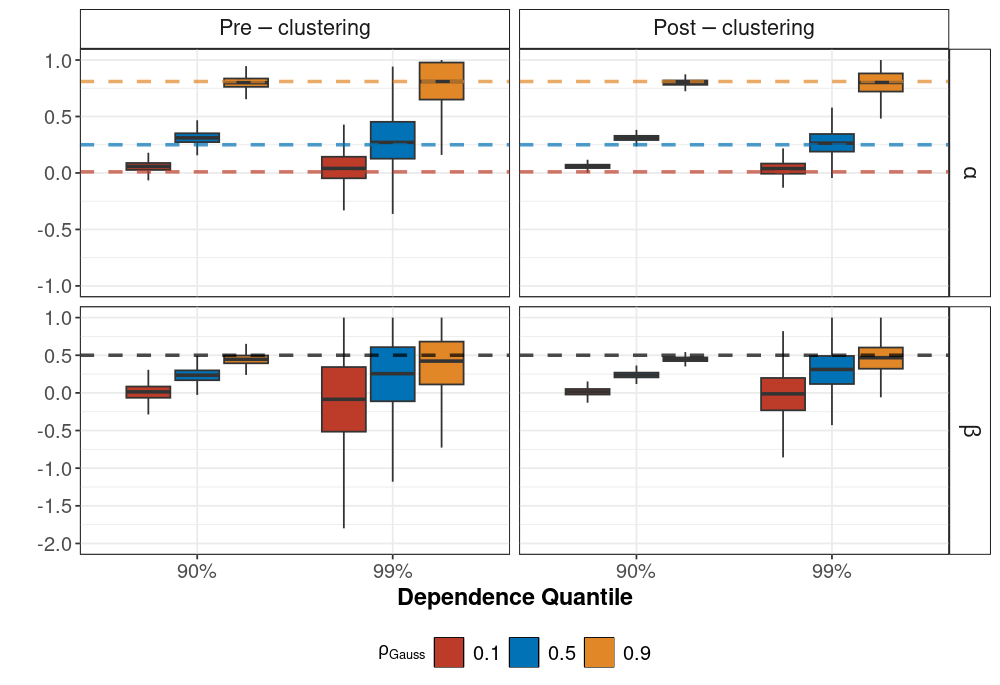
\includegraphics[width = 0.8\linewidth]{figure_1.png}
    \caption{\emph{ 
    Boxplots of estimates of $\alpha_{\mid i}$ (top) and $\beta_{\mid i}$ (bottom) for the conditional extremes model pre- and post-clustering with bivariate Gaussian data simulated at 12 sites, belonging equally to three known clusters. 
    The x-axis gives $q$, the level of the conditioning quantile used to fit the model, and the boxes are coloured by the true Gaussian copula correlation parameter, $\rho_{\text{Gauss}}^s$.
    The horizontal lines indicate the true theoretical values of $\alpha_{\mid i}$ and $\beta_{\mid i}$, with the colours for $\alpha_{\mid i}$ corresponding with the true $\rho_{\text{Gauss}}^s$ values.
    }}
   \label{fig:00_gauss_cop}
\end{figure}


\subsection{Mixture model setting}
\label{subsec:sim_mixture}

We extend our simulation design to mixtures of Gaussian and Student $t$-copulas \citep{Demarta2007-ap}, which induce asymptotic independence and asymptotic dependence, respectively, and whose dependence strength is determined by their respective correlation parameters $\rho_{\text{Gauss}}^s$ and $\rho_{\text{t}}^s \in [0, 1]$.

To obtain a sample of size $n = 1000$ from the mixture copula, at each site $s =1, \ldots, 12$, we combine $n/2 = 500$ samples from the Gaussian copula described in Section~\ref{subsec:sim_gauss} (with correlation parameter $\rhou{Gauss}^s$), and $n/2 = 500$ observations from a Student $t$-copula with 3 degrees of freedom and correlation $\rhou{t}^s$, before applying the Laplace transformation in Equation~\eqref{eq:laplace} to obtain the pairs $(Y_{1,s}, Y_{2,s})$ at site $s$.

In Section~\ref{subsubsec:sim_competing_methods}, we compare our method to the leading extremal competitor in the bivariate case \citep{Vignotto2021} and, in Section~\ref{subsubsec:sim_extension}, we show how our approach uniquely handles clustering of multivariate extremes in higher dimensions ($d > 2$).
Finally, Section~\ref{subsubsec:sim_realistic} considers a setting with $D = 60$ locations across three unequally sized clusters, and locations in the same cluster exhibiting perturbations in their correlation parameters.
Performance is evaluated using the ARI, with 500 replicated experiments per setting.

\subsubsection{Comparison to \citet{Vignotto2021}}
\label{subsubsec:sim_competing_methods}

When $d = 2$, we compare our extremal clustering method to that of \citet{Vignotto2021}.
We generate $n = 1000$ observations at $D = 12$ sites, using the mixture of Gaussian and t-copulas (with Laplace margins), as described above. 
Two clusters of sites $s = {1, \ldots, 6}$ and $s = {7, \ldots, 12}$ are defined with different values of $\rhou{t}^s$. 
We set $\rhou{t}^s = \rho_{\text{t}_1}$ for $s = 1, \ldots, 6$ and $\rhou{t}^s = \rho_{\text{t}_2}$ for $s = 7, \ldots, 12$, while $\rhou{Gauss}^s$ is the same for both clusters. 
We consider a range of extremal dependence scenarios defined over a grid of values $\left(\rhou{Gauss}^s \in \{0.1, 0.2, \ldots, 1.0\}, \rho_{\text{t}_1}^s \in \{0.1, 0.3, \ldots, 0.9\}, \rho_{\text{t}_2}^s \in \{0, 0.2, \ldots, 0.8\}\right)$.
We estimate the CE model using $q = 0.9$, and clusters were obtained using the aggregated dissimilarity matrix $M$ in Equation~\eqref{eq:aggregate_matrix}.

The results are shown in Figure~\ref{fig:01_ce_vs_vi}. 
Across the range of considered bivariate extremal dependence structures, our method consistently outperforms that of \citet{Vignotto2021}. 
Both methods have high ARI when the cluster-wise difference in $\rhou{t}^s$ is larger, since greater disparity naturally makes clusters more distinct and clustering easier. 
Both methods perform better when the Gaussian and t-copula correlations are higher.
This may be because the Gaussian copula becomes more similar to the t-copula for higher values of $\rhou{Gauss}$, thus allowing the clustering approach to focus on differences in the t-copula.

\begin{figure}[htb]
    \centering
    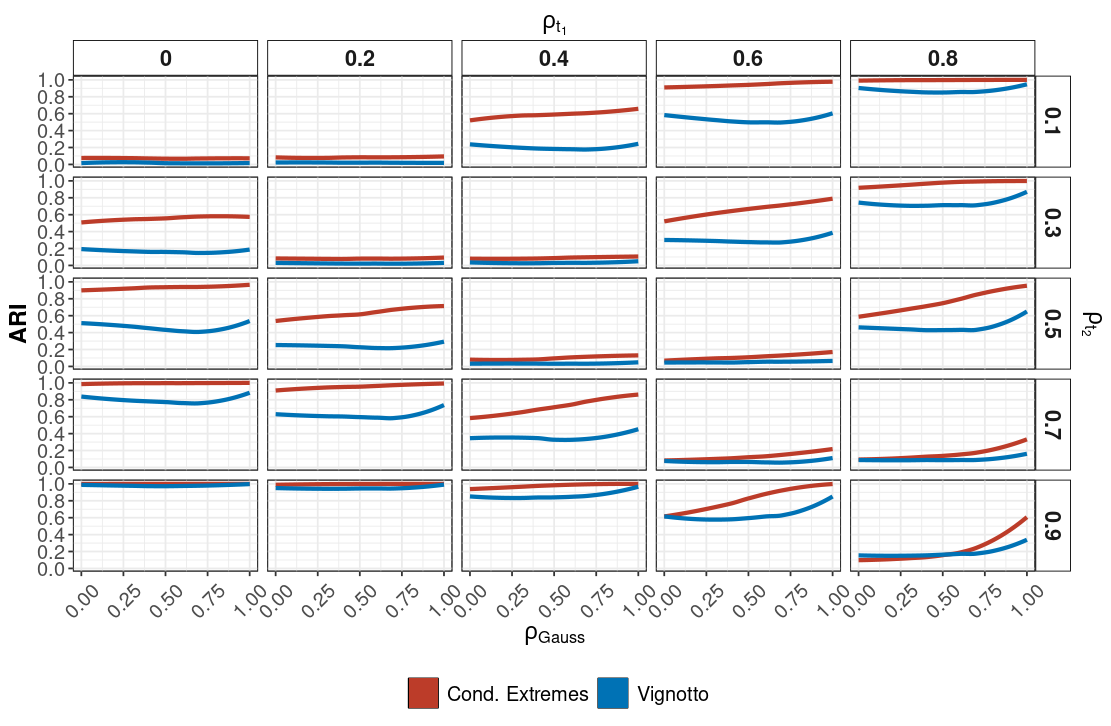
\includegraphics[width = 0.8\linewidth]{figure_2.png}
    \caption{\emph{
    Comparison of our conditional extremes-based approach and the method of \citet{Vignotto2021}.
    The x-axis represents the Gaussian correlation parameter $\rhou{Gauss}$, with facet labels indicating the t-copula correlation parameters, $\rho_{\text{t}_1}$ and $\rho_{\text{t}_2}$, for the two true clusters.
    The smoothed lines show the average ARI across bootstrap samples, for both methods, with smoothing performed using a generalised additive model.
    }}
    \label{fig:01_ce_vs_vi}
\end{figure}

\subsubsection{Extension to higher dimensions}
\label{subsubsec:sim_extension}

While the method of \citet{Vignotto2021} is restricted to $d = 2$ dimensions, our approach can be extended to $d \geq 3$ variables. 
To illustrate this, we extend the simulation study of Section~\ref{subsubsec:sim_competing_methods} by simulating at $D = 12$ locations, with two equally-sized clusters of sites each with $n = 1000$ observations per site, but now for $d = 3$ variables, using the same grid of ($\rhou{Gauss}, \rho_{\text{t}_1}, \rho_{\text{t}_2}$) values as in Section~\ref{subsubsec:sim_competing_methods}.
Our mixture copula now has three dimensions (with all pairwise correlations equal), and we fit three CE models at each site. 
Clustering is performed using the aggregated divergence matrix $M$ from Equation~\eqref{eq:aggregate_matrix}.
The results show that our proposed method performs well for $d =3$, with the same patterns in ARI emerging as in the bivariate case in Section~\ref{subsubsec:sim_competing_methods}.
In fact, performance is markedly stronger in three dimensions than in two. 
This is not surprising, as the CE fits in this setup are similar in both two and three dimensions, with the same $\rhou{t}^s$ being used across all variable pairs.
Therefore, the aggregated matrix $M$ in Equation~\eqref{eq:aggregate_matrix} is computed similarly, just averaged over more models with more data, which naturally improves clustering performance.

\begin{figure}[htb]
    \centering
    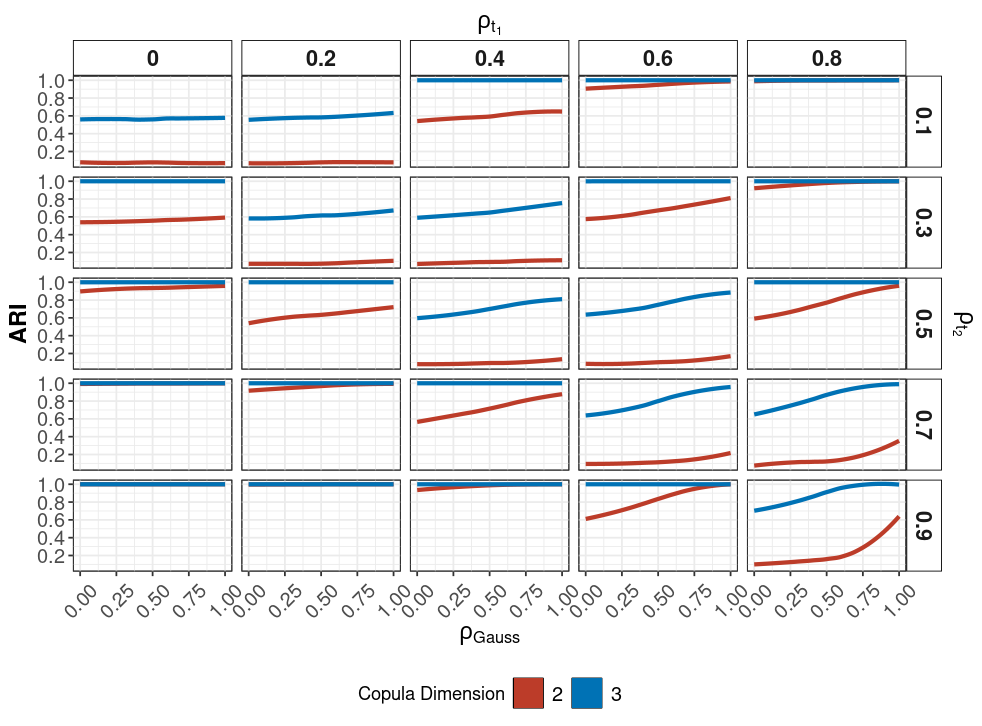
\includegraphics[width = 0.8\linewidth]{figure_3.png}
    \caption{\emph{
        Comparison of clustering performance for $d = 2$ and $d=3$ variables and two equally-sized clusters. 
        The x-axis represents the Gaussian correlation parameter $\rhou{Gauss}$ for both clusters, and the facet labels show the t-copula correlation parameters, $\rho_{\text{t}_1}$ and $\rho_{\text{t}_2}$, for the two true clusters.
        The smoothed lines show the average ARI across bootstrap samples, with smoothing performed using a generalised additive model.
    }}
   \label{fig:02_3d}
\end{figure}


% Expand to up to 5 dimensions!
To further illustrate the performance of our method in higher dimensions, we consider a specific case from the grid where $\rho_{\text{t}_1} = 0.4$ and $\rho_{\text{t}_2} = 0.5$. 
This setting presents a challenging clustering scenario in both two and three dimensions, as the cluster-wise difference in the t-copula correlation parameters is small. 
Figure~\ref{fig:02b_5d} displays the results when the dimensionality of the copula mixture is increased from $d = 2$ to $d = 5$, based on 500 simulations across all considered $\rhou{Gauss}$ values. 
Cluster accuracy improves steadily with dimension, reaching values close to 1 across all $\rhou{Gauss}$ settings when $d = 5$. 
These gains should be interpreted cautiously, since as mentioned above we use the same $\rhou{t}^s$ across all variable pairs, thus not altering the pairwise extremal dependence structure and instead increasing the amount of data as $d$ increases.
Having separate $\rhou{t}^s$ values for each variable pair would increase the complexity and signal-to-noise ratio of the clustering task, and likely reduce performance.
Nevertheless, the results demonstrate that the proposed method scales effectively to higher dimensions and performs well in multivariate settings. 

\begin{figure}[htb]
    \centering
    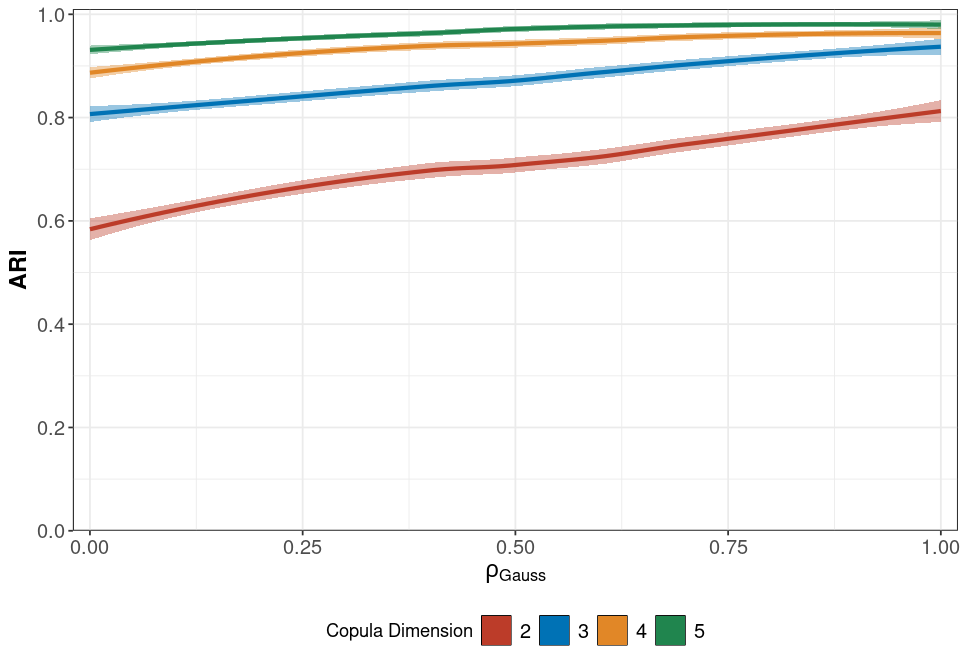
\includegraphics[width = 0.7\linewidth]{figure_4.png}
    \caption{\emph{
        Evaluation of clustering for $d = 2$ to $d = 5$ variables and two equally-sized clusters for simulations at 12 sites from a mixture of Gaussian and t-copulas.
    The t-copula correlation parameters for each true cluster were set to $\rho_{\text{t}_1} = 0.4$ and $\rho_{\text{t}_2} = 0.5$. 
A sequence of values are considered for the Gaussian correlation parameter $\rhou{Gauss}$, as represented on the x-axis.
    The smoothed lines show the average ARI and associated uncertainty across bootstrap samples, with smoothing performed using a generalised additive model.
}}
\label{fig:02b_5d}
\end{figure}

\subsubsection{Extension to more sites}
\label{subsubsec:sim_realistic}

We now design another simulation study to better mimic the structure of the Irish meteorological dataset, to be analysed in Section~\ref{sec:application}. 
Data are generated at $D = 60$ sites, each with $n = 1000$ observations of $d = 2$ variables, using the mixture of Gaussian and t-copulas.
The 60 sites are partitioned into three unequally-sized clusters of 10, 20, and 30 sites. 
At each location, the true $\rho_{\text{t}}^s$ is perturbed by adding $\text{Unif}(-0.05, 0.05)$ noise, making the clustering task more challenging.
We now have a separate t-copula correlation parameter for each of the three clusters, denoted by $\rho_{\text{t}_1}, \rho_{\text{t}_2}$, and $\rho_{\text{t}_3}$.
To reduce the dimensionality of the grid of considered copula parameter values, a constant $\rhou{Gauss} = 0.5$ is used across all sites and experiments. 

% results
The results of 500 repetitions of this simulation study are shown in Figure~\ref{fig:03_realistic}.
Similarly to the previous simulation studies, our clustering method performs well, particularly when the differences in t-copula correlation parameters between clusters are larger. 
For example, the best performance is observed where $\rho_{\text{t}_1} = 0.9, \rho_{\text{t}_2} = 0.1$, and $\rho_{\text{t}_3} = 0.5$, as the clusters are most distinct, while conversely, performance is worst for $\rho_{\text{t}_1} = 0.6, \rho_{\text{t}_2} = 0.4$, and $\rho_{\text{t}_3} = 0.5$. % \todo{Include this to aid reading of figure, is it necessary?}

\begin{figure}[htb]
    \centering
    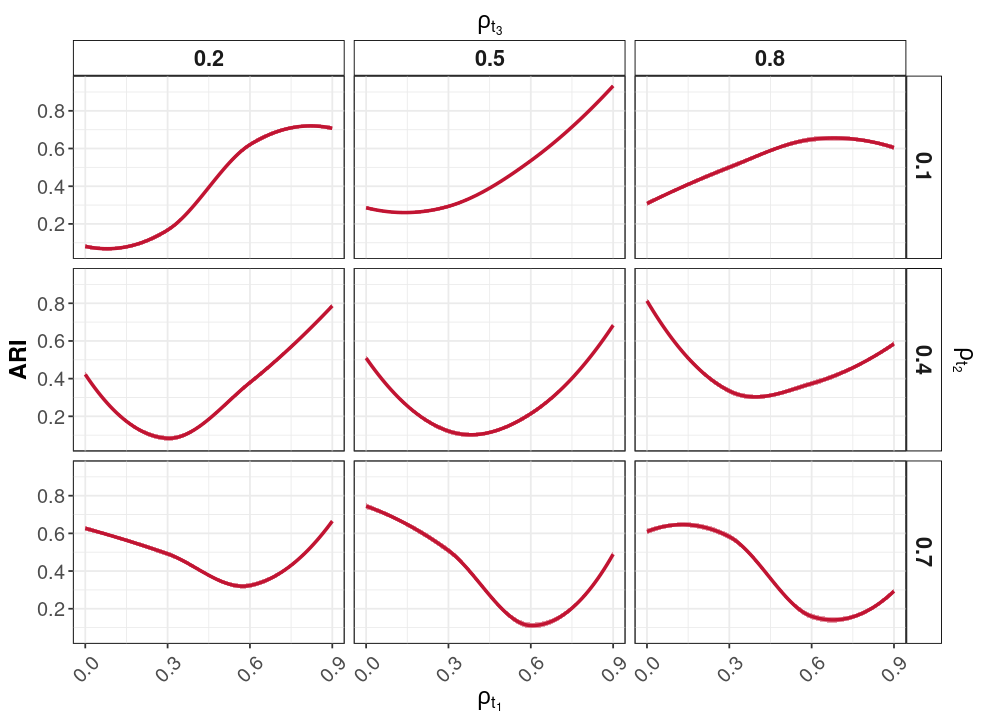
\includegraphics[width = 0.7\linewidth]{figure_5.png}
    \caption{\emph{Evaluation of clustering performance for $d = 2$ variables and three clusters of 60 locations for simulations from a mixture of Gaussian and t-copulas.
        The true x-axis and facet labels show the t-copula correlation parameters,  $\rho_{\text{t}_1}, \rho_{\text{t}_2}$, and $\rho_{\text{t}_3}$, for each of the three true clusters, for a Gaussian copula correlation of $\rhou{Gauss} = 0.5$. 
    The smoothed lines show the average ARI across bootstrap samples, with smoothing performed using a generalised additive model. 
    }}
   \label{fig:03_realistic}
\end{figure}

\section{Application to Irish meteorological data}
\label{sec:application}
% Section Intro
We now apply our extremal clustering method to meteorological observations from the Republic of Ireland. 
In Section~\ref{subsec:app_data}, we describe the precipitation and wind speed measurements used in our analysis and present exploratory analysis (using the $\chi$ statistic from Equation~\eqref{eq:chi}) on the extremal dependence between the two variables. 
In Section~\ref{subsec:app_ce}, we discuss fits of the conditional extremes (CE) model, and, in Section~\ref{subsec:app_clust}, we apply our extremal clustering approach. 

\subsection{Ireland meteorological data}
\label{subsec:app_data}

\begin{figure}[htb]
    \centering
    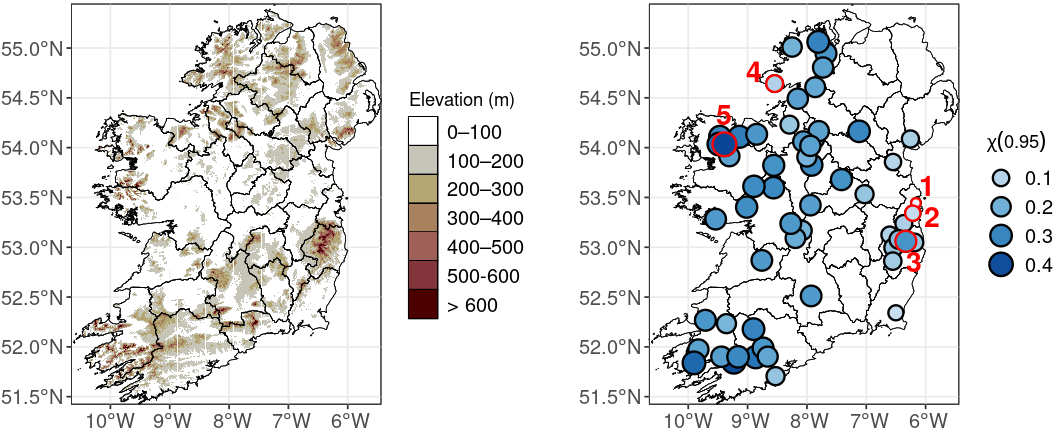
\includegraphics[width = 0.8\linewidth]{figure_6.png}
    \caption{\emph{
    Left: elevation (m) profile of Ireland.
    Right: Estimated $\chi(0.95)$ between precipitation and wind speed at all 59 locations. Darker colours and larger points indicate stronger asymptotic dependence.
    Locations in red are (1) Malahide Castle, Dublin, (2) Ringsend, Dublin, (3) Glenmacnass, Wicklow, (4) Kilcar, Donegal, and (5) Derryhillagh, Mayo.
}}
   \label{fig:chi}
\end{figure}

We analyse the joint extremal behaviour of precipitation and wind speed at $D=59$ sites across the Republic of Ireland from 1990 to 2020, inclusive. 
Precipitation and wind speed data are obtained from the Met Éireann archive \citep{metHistoricalData}, and ERA5 Reanalysis \citep{Hersbach2020}, respectively. 
Met Éireann data are irregularly spaced over space, while ERA5 provides spatial averages on a regular $0.25^{\circ} \times 0.25^{\circ}$ grid.
We match each spatial site to the grid cell in which it lies. 
The dataset spans 11,323 consecutive daily observations.

% Preprocessing
We focus on the winter months, October to March, following \citet{Vignotto2021}.
Precipitation are aggregated into weekly sums, and daily wind speed maxima are aggregated into weekly averages.
This weekly temporal scale reflects the typical lag between extreme precipitation and wind speed during storm events \citep{Bengtsson2009}, and reduces short-term temporal dependence not accounted for in our model. 
Weeks with no precipitation are excluded, resulting in 5,022 observations across all $D = 59$ sites. 

% Chi statistic
We explore the extremal dependence structure of the data using the $\chi$ statistic introduced in Equation~\eqref{eq:chi}.
Figure~\ref{fig:chi} shows empirical estimates of $\chi(0.95)$ at all 59 sites.
An elevation profile of Ireland is also shown in Figure~\ref{fig:chi}, which may help further explain some of this spatial structure.
Non-zero values are observed at almost all sites, indicating positive extremal dependence between precipitation and wind speed. 
In practical terms, this suggests that extreme wind speeds tend to be accompanied by high precipitation, and vice versa. 
A clear spatial pattern emerges: extremal dependence is strongest in the south west, with the highest values along the Atlantic coast, notably in counties Kerry, Galway, Mayo, and Donegal, and weaker along the east coast, in Dublin, Wexford, and Louth. 
The highest $\chi(0.95)$ value (0.414) is observed at Derryhillagh in Mayo (Figure~\ref{fig:chi}, location (5)), while the lowest (0.0005) is at Malahide Castle in Dublin (Figure~\ref{fig:chi}, location (1); hereafter `Malahide').

Some spatial outliers are also apparent. 
Kilcar in Donegal (Figure~\ref{fig:chi}, location (4)) has a relatively low $\chi(0.95)$ value (0.109), despite its west-coast location, while some sites in county Wicklow show unusually high values for the east, particularly Glenmacnass (Figure~\ref{fig:chi}, location (3); 0.268).
The latter may be related to the influence of the Wicklow Mountains, as reflected in the elevation profile (Figure~\ref{fig:chi}). 
It may be of interest to investigate if these outliers in $\chi(0.95)$ are reflected in the CE model parameter estimates, and whether clustering can identify them.
These results indicate distinct regional patterns of extremal dependence, as well as notable outliers, motivating the use of our extremal clustering framework to characterise and interpret this spatial structure more formally. 

\subsection{Conditional extremes estimates}
\label{subsec:app_ce}

% Procedure and results pre-clustering (choice of quantile)
We transform the precipitation and wind speed data, separately at each location, to Laplace margins, with the empirical rank transform replacing $F_{X_i}$ in Equation~\eqref{eq:laplace}.
To select an appropriate quantile level $q$ for fitting the CE model (see Section~\ref{subsec:ce_model}), we estimate the parameters $(\alpha_{\mid i}, \beta_{\mid i})$ at a sequence of levels $q$, to identify the lowest $q$ beyond which parameter estimates appear stable.
Estimates are generally stable for both models, i.e.,\@ precipitation conditional on wind speed and vice versa, down to $q = 0.85$, with similar maximum likelihood estimates across 500 bootstrap samples for $(\alpha_{\mid i}, \beta_{\mid i})$.
Threshold stability plots for the CE fits at the five locations highlighted in Figure~\ref{fig:chi} are included in Figures~\ref{fig:boot_quantiles_malahide} -- \ref{fig:boot_quantiles_derryhillagh} of the supplementary materials.
Therefore, we fix $q = 0.85$ for the subsequent analysis.
In Figure~\ref{fig:clust_sens}, we show that our estimated extremal clustering is robust to the choice of $q$, with estimates shown for $q = 0.85, 0.88$, and $0.90$.

The estimated site-wise CE parameters are shown in Figure~\ref{fig:a_b_vals}.
Although interpretation is challenging due to variability in the estimates, as with the $\chi(0.95)$ estimates (Figure~\ref{fig:chi}), we observe some evidence of increasing $\alpha_{\mid i}$ values for both variables towards the west and south.
To mitigate uncertainty and aid interpretation, we cluster the locations using our extremal clustering approach. 

\begin{figure}[htb]
    \centering
    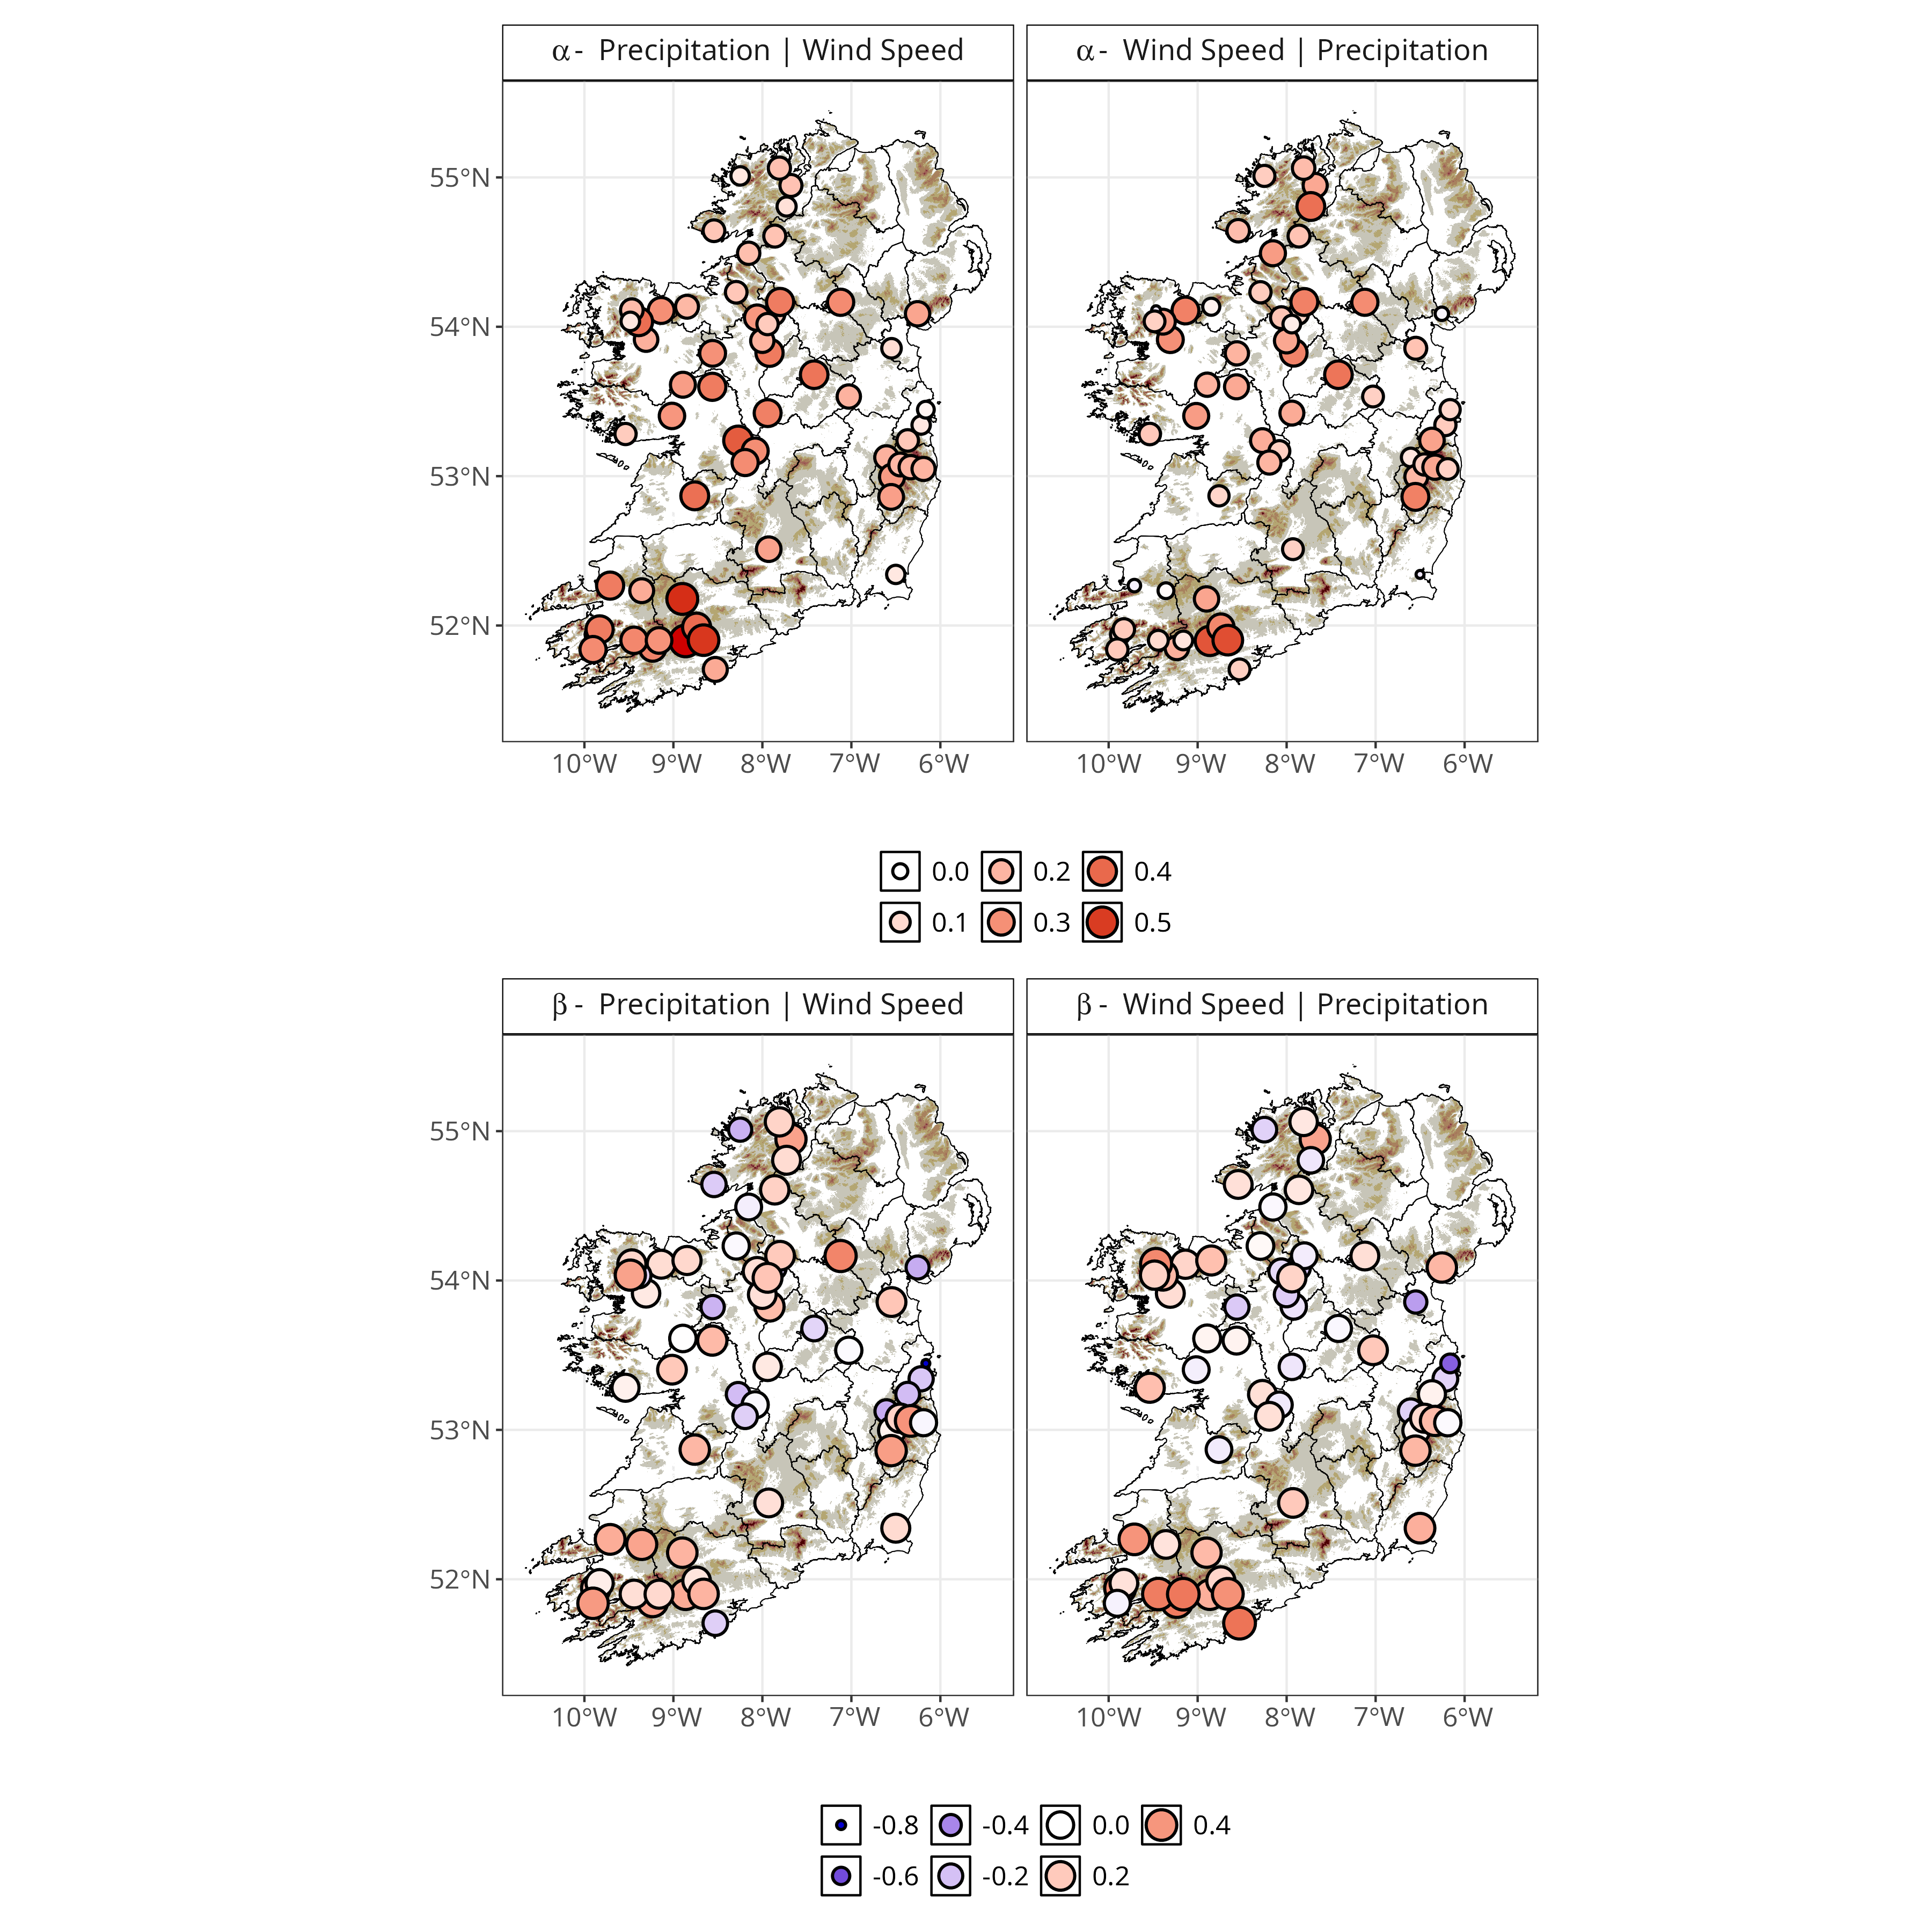
\includegraphics[width = 0.8\linewidth]{figure_7.png}
    \caption{\emph{
        Maps of site-wise estimated model parameters $\alpha_{\mid i, s}$ (top) and $\beta_{\mid i, s}$ (bottom) for precipitation conditional on wind speed (left) and wind speed conditional on precipitation (right).
        The colour scale is the same for both variables, with darker red and larger points indicating larger positive values of $\alpha$ and $\beta$, and darker blue and smaller points indicating smaller negative values.
   }}
   \label{fig:a_b_vals}
\end{figure}


\subsection{Clustering}
\label{subsec:app_clust}

We cluster the locations using the aggregated dissimilarity matrix $M$ as defined in Equation~\eqref{eq:aggregate_matrix}, and separately for each individual matrix $M^{(i)}, i = 1, 2$, as in Equation~\eqref{eq:distance_matrix}.
The number of clusters $k$ is chosen via the method in Section~\ref{subsec:clustering}, using the elbow plot of the $\mathrm{TWGSS}$. 
For all three clustering scenarios, clear elbows are observed at $k = 3$.
The elbow plots are provided in Figure~\ref{fig:elbow_plots} of the supplementary materials. 

The resulting cluster estimates are displayed in Figure~\ref{fig:clust_sol}.  
Across all three choices of dissimilarity matrix, the estimated clusters are broadly consistent, with three spatially distinct groups emerging.  
This spatial coherence is notable given that no explicit spatial information was used in model fitting or in the clustering, suggesting that the CE model parameters capture meaningful spatial structure in the extremal dependence of the data. 

When interpreting the clusters, we observe a clear contrast between the east and west coasts, separated by a central cluster.  
For precipitation conditional on wind speed, the clustering is somewhat less distinct, with the central cluster extending more extensively into parts of Galway, Mayo, and Donegal on the west coast.  
There are also notable outliers in the clusters, which we further discuss below. 

\begin{figure}[htb]
    \centering
    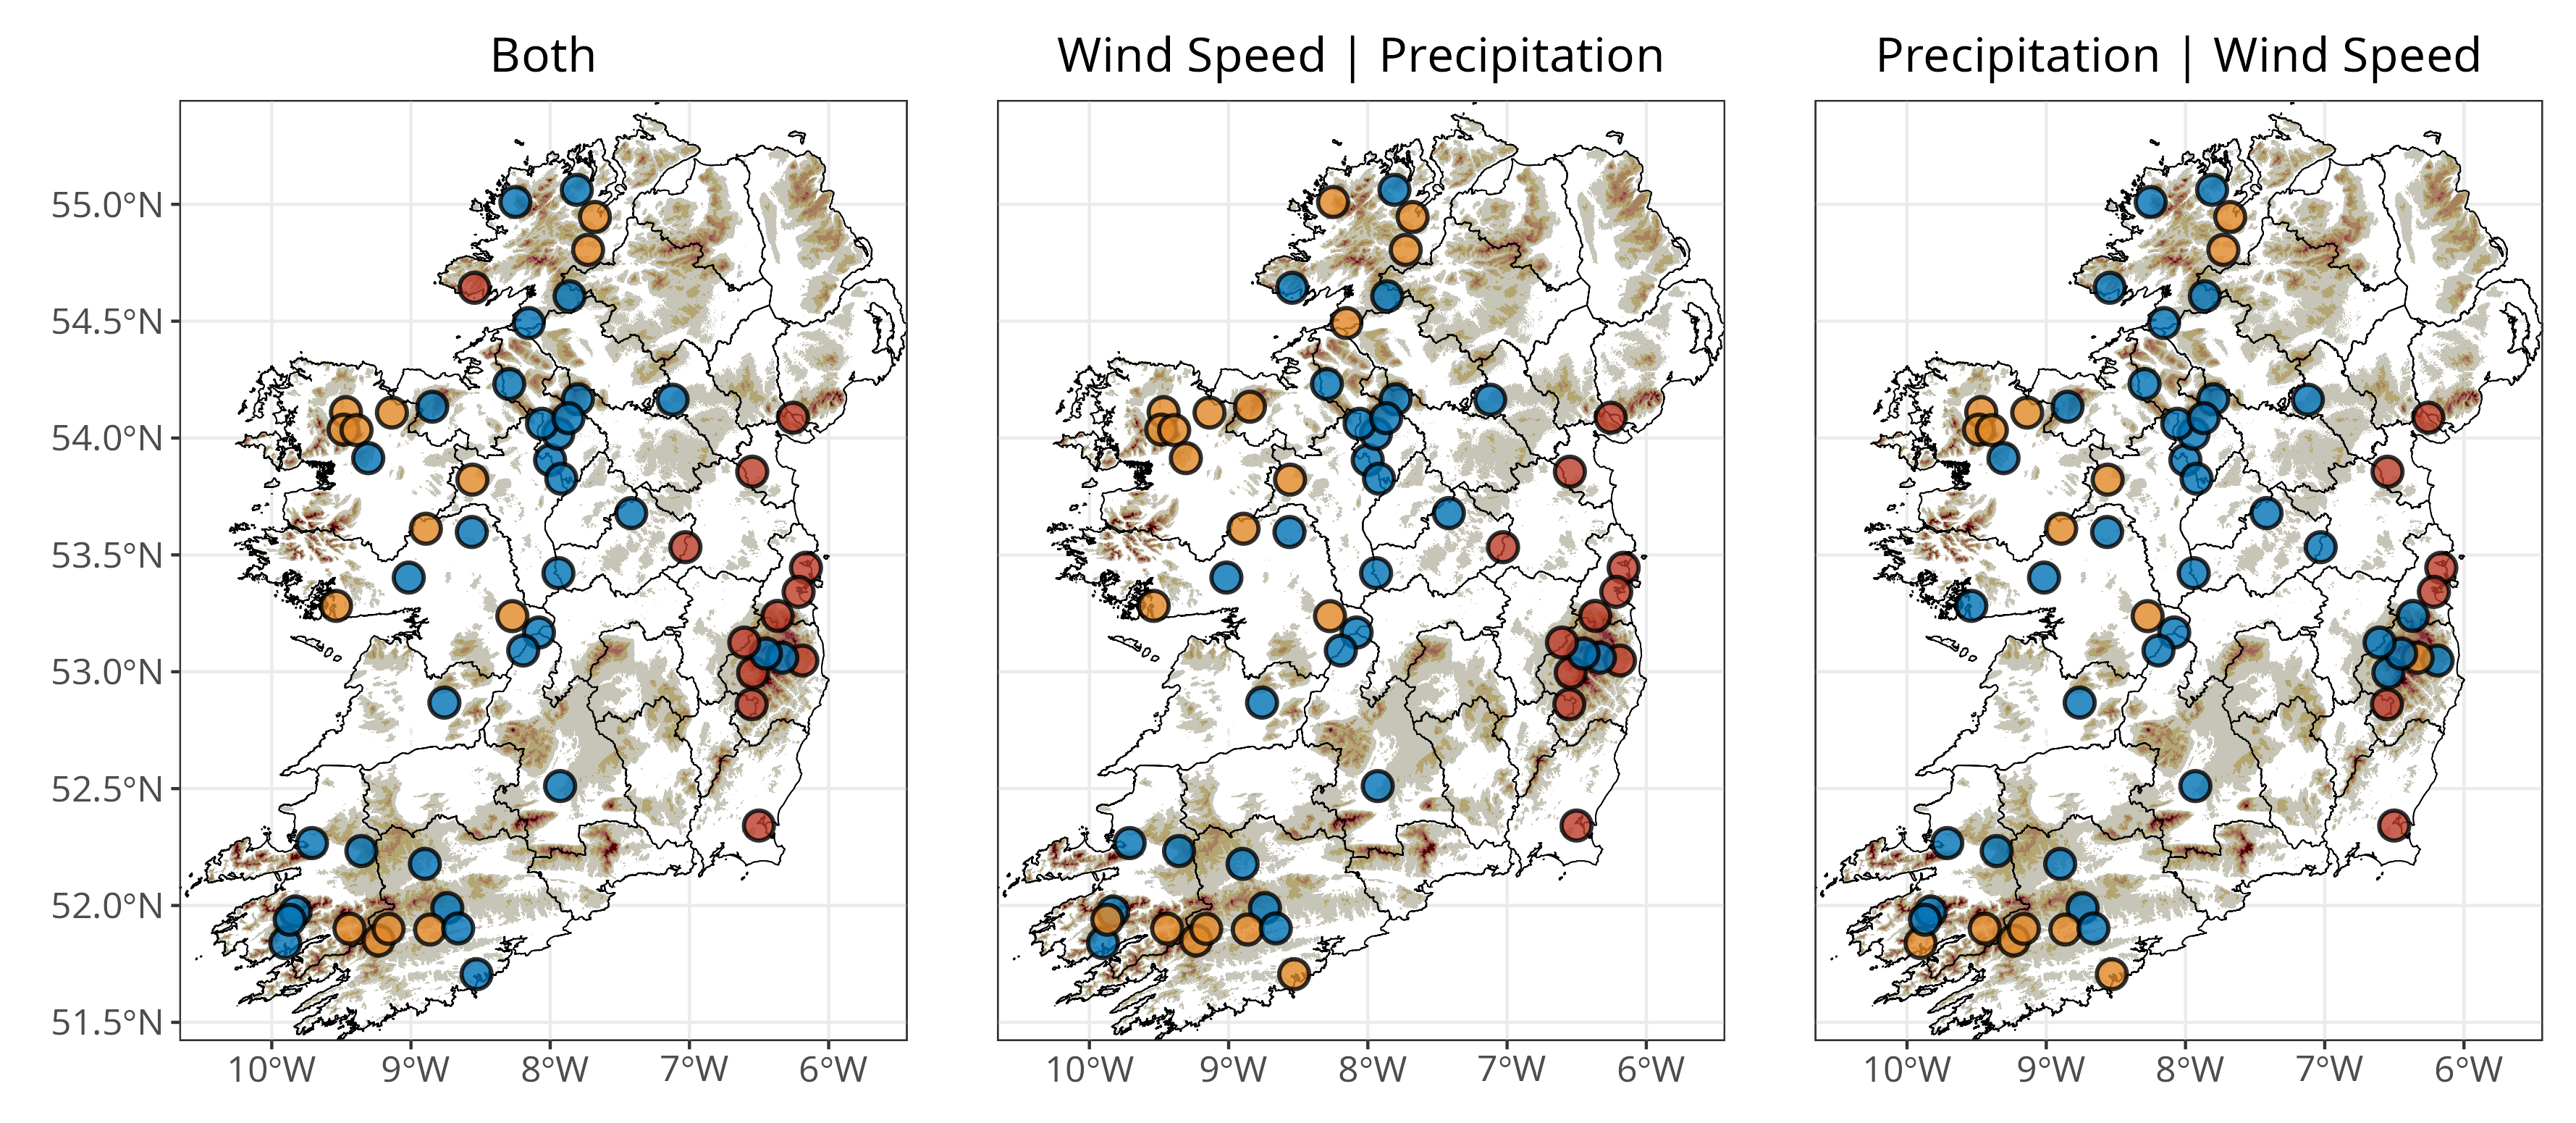
\includegraphics[width = 0.8\linewidth]{figure_8.png}
    \caption{\emph{
    Extremal cluster estimates using the dissimilarity matrix for wind speed conditional on precipitation (centre), precipitation conditional on wind speed (right), and the combined dissimilarity matrix (left). 
    Sites are coloured by cluster label.
}}
\label{fig:clust_sol}
\end{figure}

\begin{figure}[htb]
    \centering
    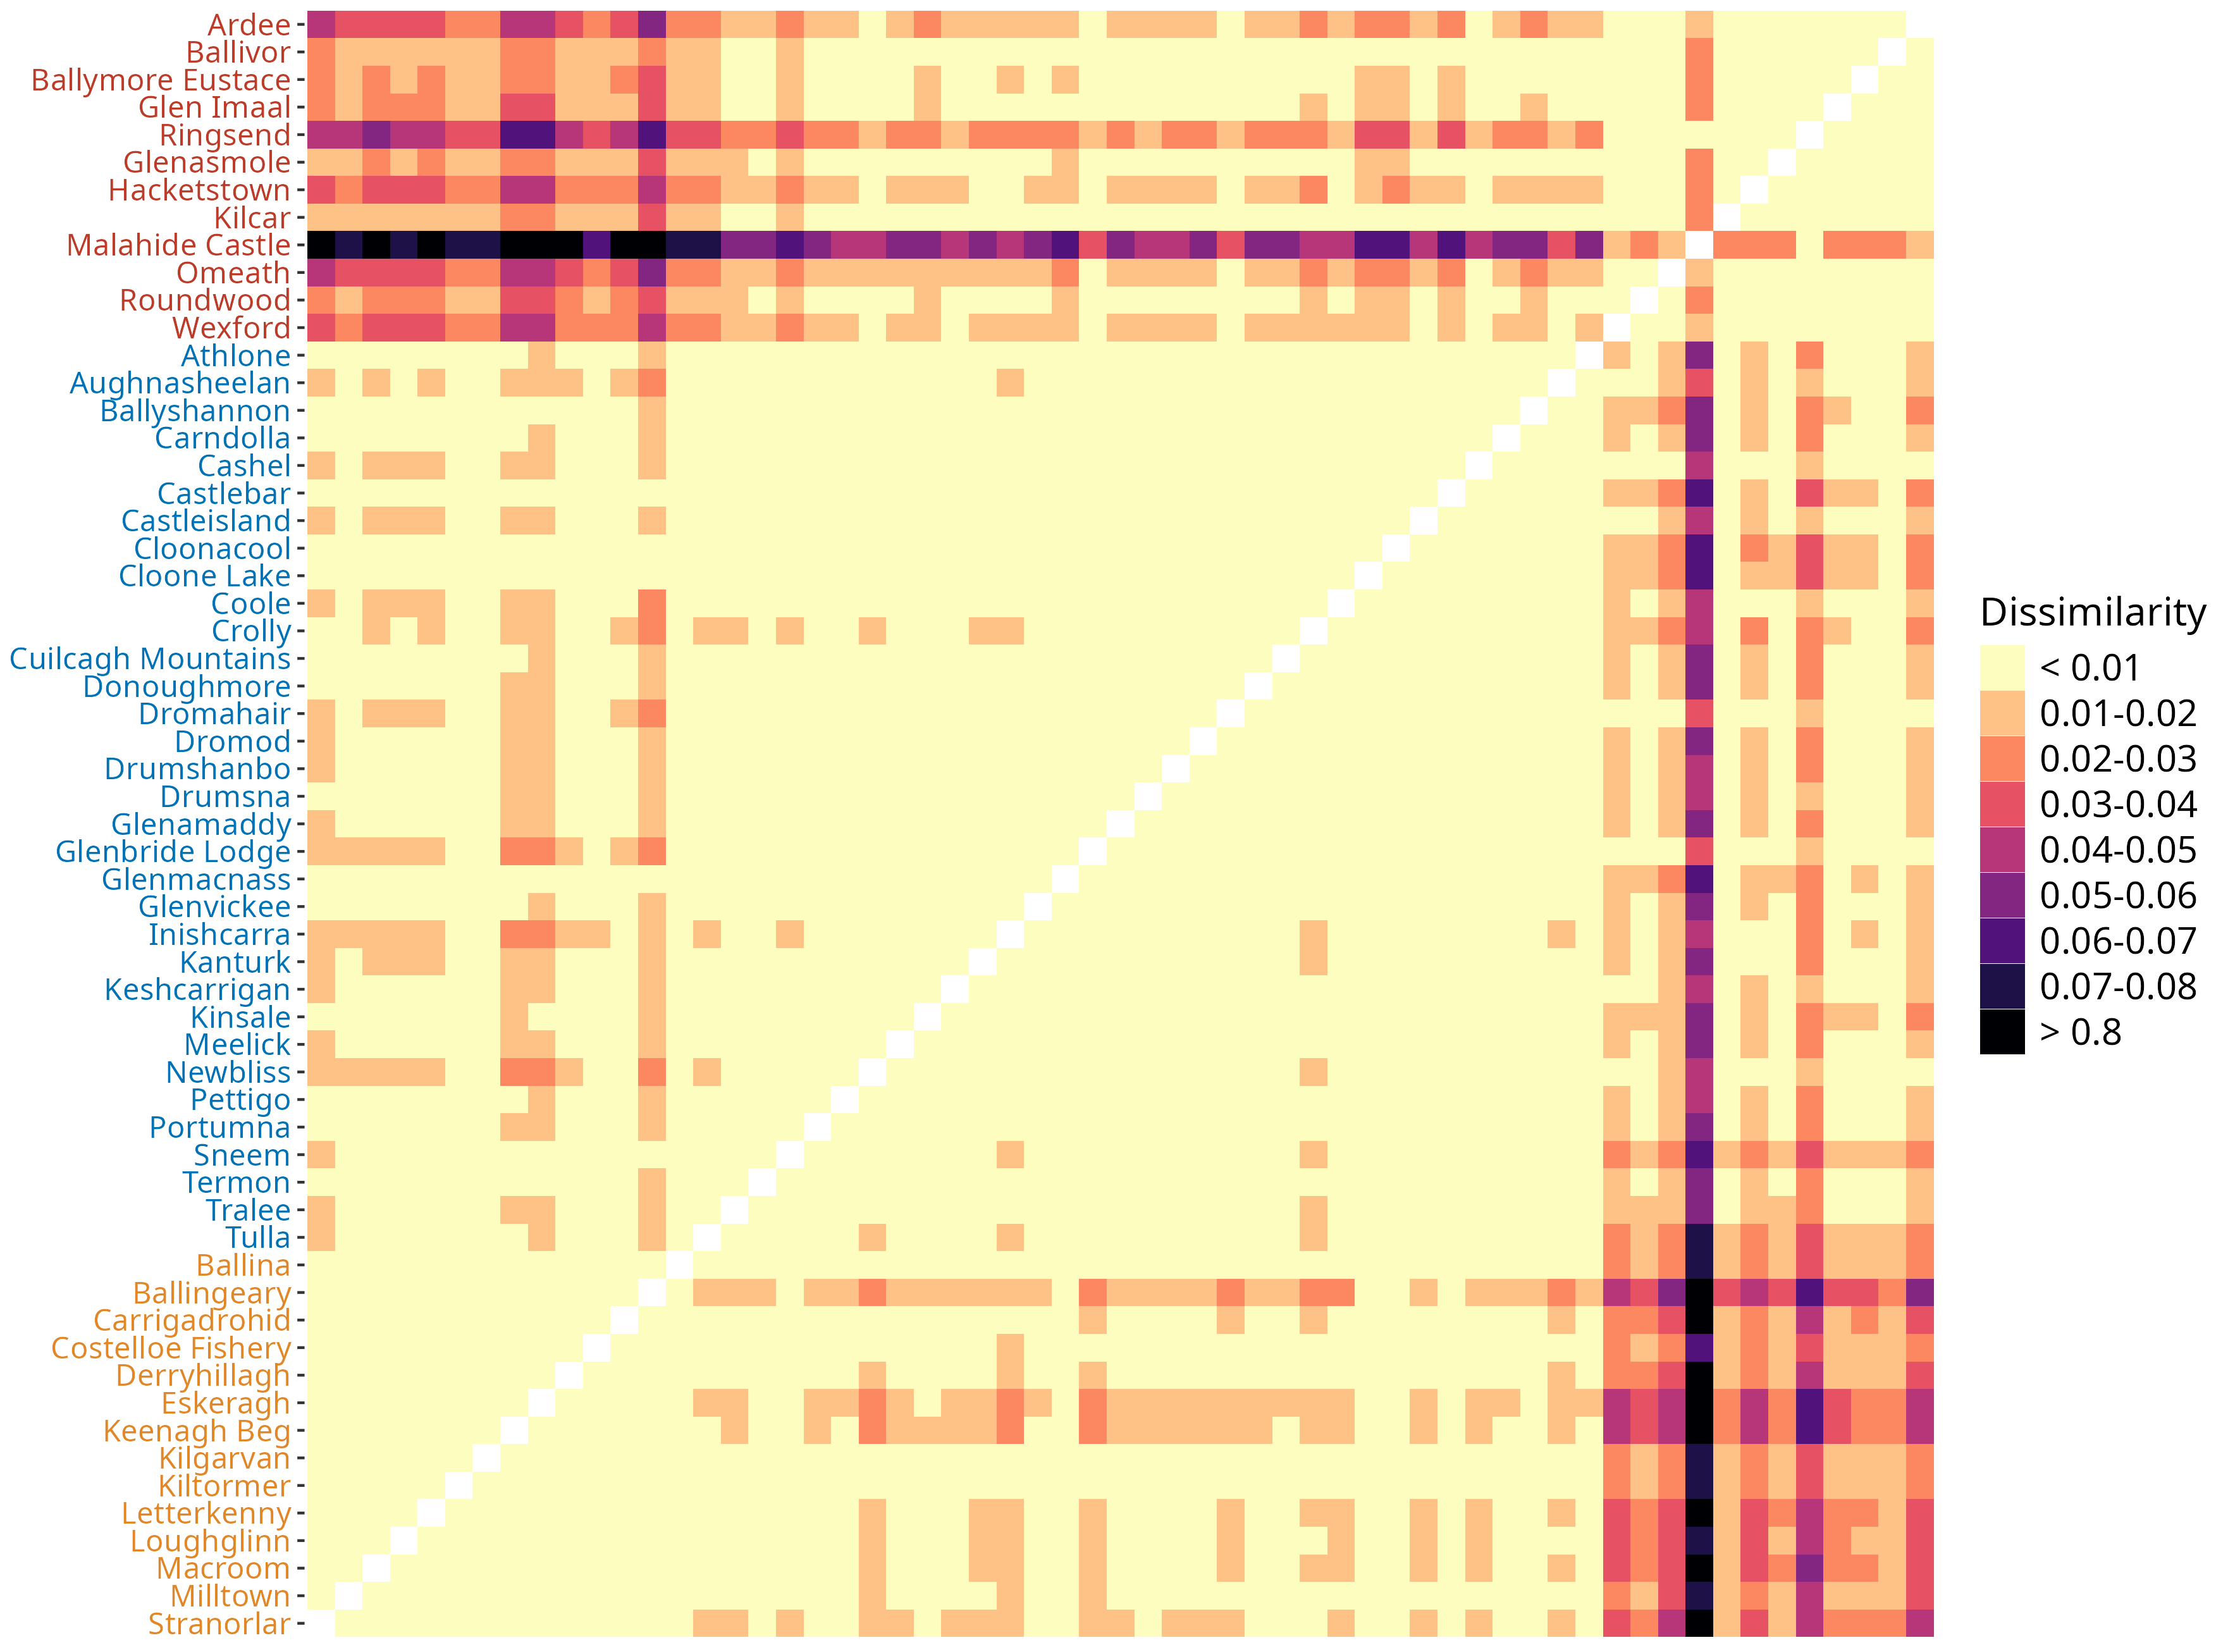
\includegraphics[width = 1.0\linewidth]{figure_9.png}
    \caption{\emph{
    Heatmap of the estimated aggregated dissimilarity matrix $M$.
The names of each site are coloured and ordered according to their estimated cluster labels, matching that of Figure \ref{fig:clust_sol}. 
The dissimilarity colour scale is shown on the right, with darker colours indicating larger values.
}}
\label{fig:dist_heatmap}
\end{figure}

% Analysis of dissimilarity matrix
In Figure~\ref{fig:dist_heatmap}, we visualise the dissimilarity matrix for the aggregated clusters (see left panel of Figure~\ref{fig:clust_sol}).
The clusters are quite distinct, with the dissimilarity between clusters being much larger than within-cluster dissimilarity, which rarely exceeds 0.01.
In particular, the difference between the eastern and western clusters is quite pronounced, with the intermediate central cluster acting as somewhat of a `buffer' between the two.
In contrast, the western and central clusters seem to be quite close, in that we observe many small inter-cluster pairwise dissimilarities between them. 
This indicates that allocation between the two is not always clear-cut and for several sites is nearly interchangeable, as observed in  the variable-specific estimated clusters in Figure~\ref{fig:clust_sol} and in the quantile sensitivity analysis in Figure~\ref{fig:clust_sens}, where membership between the two often switches. 
Also, if we only fit two clusters, we find that most of the central cluster members are assigned to the western cluster, reflecting this less obvious separation between the two compared to the more markedly different eastern cluster. 
A noticeable outlier in the dissimilarity matrix is Malahide, which we previously identified as having the lowest $\chi(0.95)$ value  in Figure~\ref{fig:chi}. 
Even within its own cluster, Malahide shows a relatively high dissimilarity to the other sites. 
Indeed, if we set $k=4$, Malahide becomes its own cluster (clustering results for $k=2$ and $k=4$ are provided in Figure~\ref{fig:cluster_dqu_k_2_4} of the supplementary materials).
Malahide also has the lowest mean weekly precipitation of any site; the second lowest is Ringsend, also in county Dublin (Figure~\ref{fig:chi} location (2)), which is the site closest to Malahide in terms of our dissimilarity measure. 
Finally, Malahide has very low $\chi(0.95)$ (Figure~\ref{fig:chi}) and $\alpha_{\mid i}$ (Figure~\ref{fig:a_b_vals}) estimates. 
Together, this may explain why we observe such outlying behaviour for Malahide.
Finally, Kilcar in County Donegal is the member of the eastern cluster with the smallest dissimilarity to the western cluster members.
This may reflect its geographic location in northwest Ireland, despite it's low $\chi(0.95)$ value (Figure~\ref{fig:chi}) relative to other west-coast sites.

\begin{figure}[htb]
    \centering
    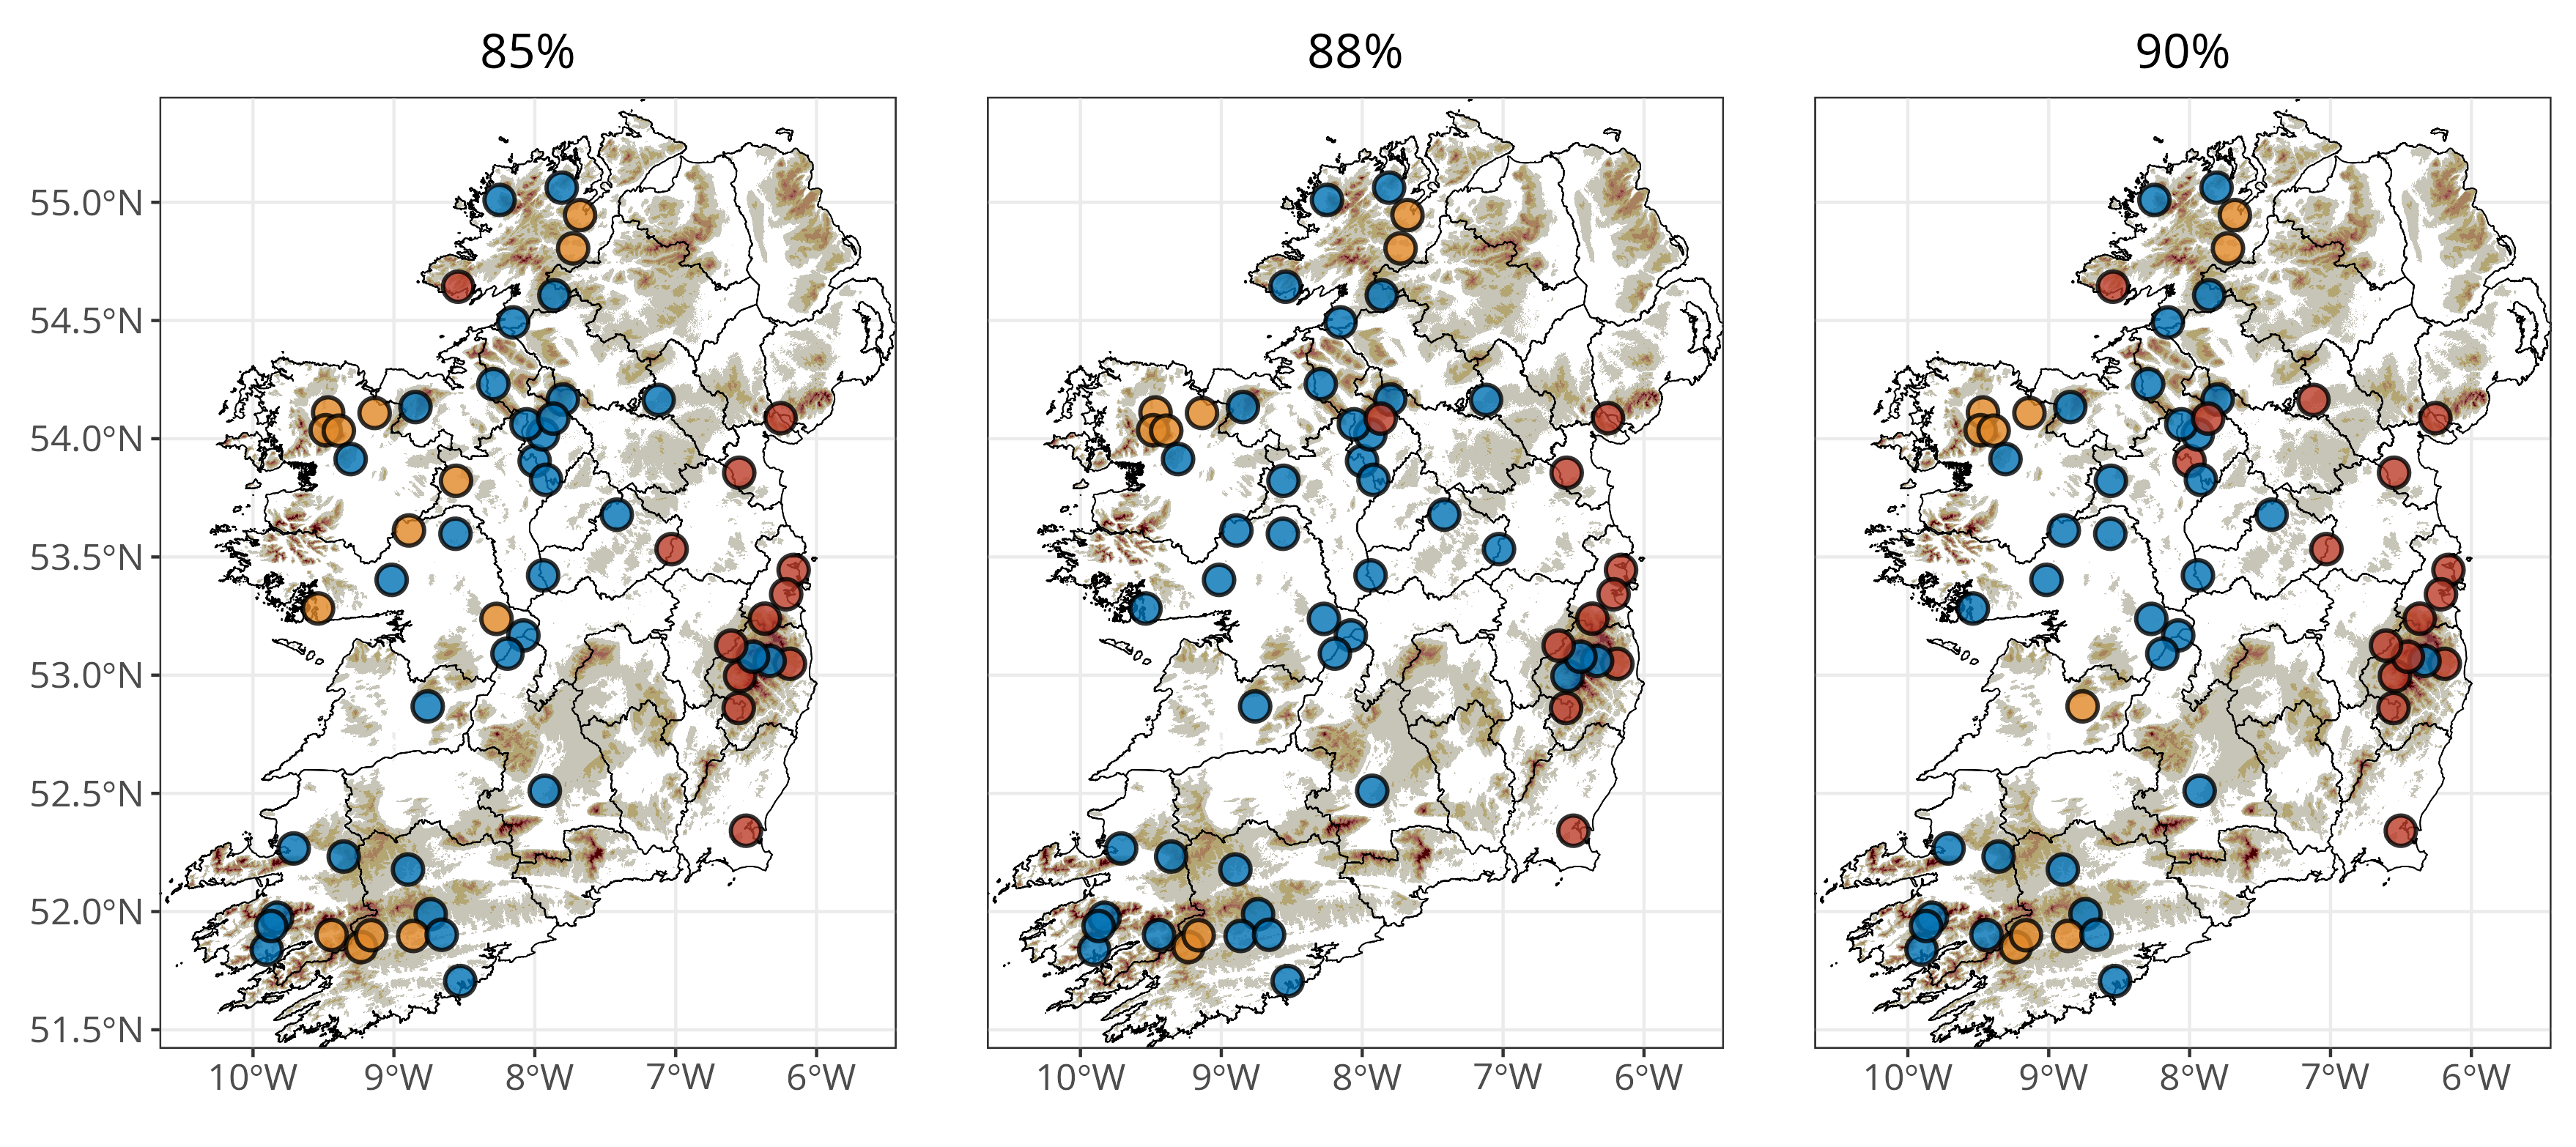
\includegraphics[width = 0.85\linewidth]{figure_10.png}
    \caption{\emph{
    Estimated extremal clusters with the conditional extremes model parameters estimated at $q = 0.85, q = 0.88$ and $q = 0.9$ quantiles, using the aggregated dissimilarity matrix. 
    Sites are coloured by cluster label. 
}}
\label{fig:clust_sens}
\end{figure}


% Sensitivity Analysis (to choice of DQU)
We perform a sensitivity analysis of the estimated clusters (with the aggregated dissimilarity matrix) to the choice of quantile level $q \in \{0.85, 0.88, 0.90\}$, in Figure~\ref{fig:clust_sens}.
The estimated clusters are similar across the three values of $q$, with some small differences. 
Noticeably, the earlier identified outlier at Kilcar in county Donegal is assigned to the eastern cluster when $q = 0.85$ and $q = 0.90$, but to the central cluster when $q = 0.88$.
Also, there are more sites in the western cluster when $q = 0.85$, with some sites moving to the central cluster for $q = 0.88$.
Interestingly, some of these sites then move back to the western cluster for $q = 0.90$.
Apart from these observations, the estimated clusters are generally quite similar across the three quantile levels, and so we conclude that our clustering method is relatively robust to the choice of quantile level.

\section{Discussion}
\label{sec:discuss}

% Quick summary
In this paper, we introduced a novel method for clustering multivariate extremes.
We proposed the expected conditional $\JSGa{}$ divergence \citep{Nielsen2019} as a measure of dissimilarity between multivariate conditional extremes (CE) models \citep{Heffernan2004}.
We leveraged the commonly-applied working Gaussian assumption to derive a closed-form expression for the $\JSGa{}$ divergence.
Efficient k-medoids clustering was then performed on the dissimilarity matrix derived from this measure. 
In our simulation study, a bivariate Gaussian copula example illustrated that our clustering method reduces parameter uncertainty and bias when the CE model is re-fitted with data pooled post-clustering.
Using mixtures of Gaussian and $t$-copulas, we showed that our method outperforms the method of \citet{Vignotto2021} across a range of bivariate extremal dependence scenarios.
Our method was also shown to be uniquely extendable to $d > 2$ dimensions. 
We applied our extremal clustering method to Irish meteorological data, consisting of 59 locations with weekly rainfall and wind speed observations.
Without explicitly incorporating spatial information, three clusters with distinct spatial patterns were identified, with well separated clusters representing the east and west coasts and the centre of Ireland.

% Extension
While we focused on a spatial application in this work, our method is more generally applicable to any setting where clustering of multivariate extremal dependence is desired.
For instance, it could be applied to clinical trial or public health data to cluster patients based on the tail dependence structure of their symptoms or biomarker measurements.
A neuroscience application was explored in \citet{Talento2025}, where the CE framework was used to highlight differences in the tail dependence of electroencephalogram (EEG) signals for seizure-prone and seizure-absent subjects. 
However, they used pre-defined clusters. Hence, we may expect our approach to be useful in similar applications, to identify subjects who have undergone extreme brain events, e.g., seizures.
In financial applications, we could cluster time periods according to the extremal dependence of log-returns of different assets, offering potential insights for portfolio management and risk assessment.

% Limitations: Gaussian assumption
While the residual Gaussian assumption on which our method relies may not hold for all datasets, our clustering approach showed good performance for all settings in Section~\ref{sec:sim}.
A possible alternative is to employ the generalised and asymmetric multivariate Gaussian distribution used in \citet{Farrell2025}. 
While this does not permit a closed-form divergence, our extremal clustering method could still be used, with costly numerical techniques used to estimate the dissimilarity matrix.
Indeed, if choosing to forgo this Gaussian assumption, it may be preferable to use the standard Jensen-Shannon divergence in place of the $\JSGa{}$ divergence, since the former is bounded \citep{Thiagarajan2025}.

% Limitations: Uncertainty
Another important limitation of our method is in its treatment of uncertainty.
We do not propagate uncertainty in the CE model estimates through to the clustering. 
To account for this, one possible approach is to use the bootstrap method of \citet{Heffernan2004} to generate samples of CE model estimates, and compute our dissimilarity matrix for each sample. 
We could then produce a distribution of dissimilarity matrices, and use these to compute a distribution of estimated clusters.
However, this would be computationally expensive, and so would compromise one of the main advantages of our method, namely its computational efficiency.

% Future work
In this work, we implicitly assume spatial stationarity in the extremal dependence structure, as we fit a separate CE model at each location.
Extensions of the CE model have been proposed, such as those incorporating covariates \citep{Richards2023} and spatio- and spatio-temporal representations of the CE parameters \citep{Simpson2021, Wadsworth2022}.
These could be incorporated into our clustering framework, but care must be taken to ensure that the residual Gaussian assumption still holds, or that an appropriate alternative dissimilarity is used, as discussed above.
Another approach to dealing with the uncertainty in the clustering solution would be to adopt a Bayesian perspective.
By placing priors on the CE model parameters, we could obtain posterior distributions for these parameters, which could be used to compute a distribution of dissimilarity matrices and clustering solutions.
Approaches such as that of \citet{Rohrbeck2021} have used a Reversible-Jump MCMC scheme to perform Bayesian clustering for spatial extremes, which does not require the number of clusters to be specified in advance.



% \section*{Acknowledgements}
% 
% \if0\blind
% {%
% Patrick O'Toole is supported by a scholarship from the EPSRC Centre for Doctoral Training in Statistical Applied Mathematics at Bath (SAMBa), under the project EP/S022945/1.
% We acknowledge the use of the ERA5 reanalysis dataset, available from the Copernicus Climate Change Service (C3S) Climate Data Store (CDS) (\url{https://cds.climate.copernicus.eu/}). 
% We also acknowledge the use of the Irish meteorological dataset obtained from Met Éireann (\url{https://www.met.ie/climate/available-data/historical-data}).
% } 
% \else
% {%
% We acknowledge the use of the ERA5 reanalysis dataset, available from the Copernicus Climate Change Service (C3S) Climate Data Store (CDS) (\url{https://cds.climate.copernicus.eu/}). 
% We also acknowledge the use of the Irish meteorological dataset obtained from Met Éireann (\url{https://www.met.ie/climate/available-data/historical-data}).
% }
% \fi


\begin{center}
{\large\bf SUPPLEMENTARY MATERIAL}
\end{center}

\begin{description}

  \item[PDF Supplement:] This supplement contains additional plots for the motivating data application in Section~\ref{subsec:app_clust} of the main paper, including elbow plots for choosing the number of clusters, clustering solutions for $k=2$ and $k=4$ clusters, and threshold stability plots for the conditional extremes model fits for the five locations highlighted in Figure~\ref{fig:chi}.

  \item[Data and R code:] The proposed methods are made available in an R package (link omitted for blind review).
    The analysis code used in the paper and the data are available upon request from the corresponding author.

\end{description}

% \typeout{=== TEX DIAGNOSTIC: before checking .bbl ===}
% \IfFileExists{manuscript_anonymous.bbl}{%
%   \typeout{=== TEX DIAGNOSTIC: BBL FILE FOUND ===}%
% }{%
%   \typeout{=== TEX DIAGNOSTIC: BBL FILE NOT FOUND ===}%
% }
% \typeout{=== TEX DIAGNOSTIC: after check ===}

% \bibliographystyle{apalike}
{\small
% \bibliography{library.bib}
\input{manuscript_anonymous.bbl}
}

\clearpage

\end{document}

}

\clearpage

\end{document}

}

\clearpage

\end{document}

}

\clearpage

\end{document}
